\documentclass[a4paper,12pt]{article}

\usepackage{libYesdoc}
\usepackage{lstlistingStyles}

% Bibliografía
\usepackage[
backend=biber,
style=authortitle,
sorting=nty
]{biblatex}
\bibliography{biblio}

\raggedbottom %para evitar espacio en blanco al añadir una imagen

\begin{document}
	%Cabecera y Pie de Página
	\headheight=.3in
	\renewcommand{\headrulewidth}{0.5pt} % grosor 
	%\addtolength{\headheight}{0.2pt} % espacio 
	\lhead[]{}
	\chead[]{}
	\cfoot[]{}
	\rfoot[\thepage]{\thepage}%info
	\renewcommand{\footrulewidth}{0.5pt}

\input{caratula}

\tableofcontents
\addcontentsline{toc}{section}{Trabajo Práctico N° 1: Desarrollo de un Sistema de Información real}

\section*{Trabajo Práctico N° 1: Desarrollo de un Sistema de Información real}

\section{Definición de requerimientos}

\subsection{Presentación del proyecto}
El proyecto aquí detallado permitirá a toda persona la unificación y centralización de la totalidad de su información relacionada con el bienestar y salud, poniéndola a disposición de la misma o de terceros autorizados.

Proporcionará el ingreso de distintos tipos de datos y estudios que serán gestionados personalmente, presentando un medio de uso simple, ágil e intuitivo para alentar y facilitar su uso.
Uno de los objetivos es que la persona pueda hacer uso de esta aplicación desde cualquier lugar del mundo y en cualquier momento, a través de Internet, usando un dispositivo móvil o una PC.

Brindará al propietario de la información, la posibilidad  de interactuar con los profesionales médicos de su preferencia, brindándole a ellos los permisos adecuados para realizar consultas, seguimientos, aportar comentarios y/o dar conclusiones según sus requerimientos.

El proyecto estará dirigido por los lineamientos del software libre, para lo cual no sólo se hará uso de tecnologías textit{open source}, sino que también estará públicamente disponible.


\subsection{Relevamiento general}

\subsubsection{Relevamiento de la organización}

Actualmente puede observarse que en forma generalizada, tanto en nuestra provincia, país y mayormente en todo el mundo, los hospitales y organizaciones de salud manejan la información del paciente mediante historias clínicas dentro de la misma institución en forma privada, limitando el acceso del paciente a la misma.
Esto plantea una idea falsa de la universalidad de la información, ya que si una persona se hace atender en un centro médico, tendrá los datos de los estudios que se ha realizado en ese lugar; sin embargo, no tendrá acceso a los que pudo haberse realizado en otras instituciones en el pasado, ni podrá brindar toda esta información a los futuros centros médicos a los que asista.

En el mundo se ha comenzado a fomentar la idea de una historia clínica universal, e incluso hay lugares en los cuales se exige a los centros médicos que hagan uso de un sistema centralizada de  información.
El problema es que sigue siendo una idea o punto de vista centrado en los centros médicos y no en la personas.

Hoy en día existen aplicaciones que brindan una solución parcial al problema antes mencionado, pero no permiten al usuario el control y disposición en forma completa de su información, ya que carecen de la posibilidad de hacer uso de los mismos libremente (por ejemplo, al poder compartirla con profesionales médicos de su preferencia), de migrar sus datos a los sistemas que consideren oportunos, y de manejar la privacidad de la información sin tener que aceptar obligatoriamente los términos y condiciones de empresas que lucren o se reserven derechos sobre éstos.

Este proyecto tiene por objetivo resolver las falencias detectadas en el contexto mundial actual, permitiendo que el control de la historia clínica pase a manos de la persona, propietaria real de los datos.


\subsubsection{Relevamiento de las funciones detectadas}
En este apartado se presentarán los conceptos básicos de Carpeta de Salud Personal, se expondrá el contexto actual utilizando como ejemplo el Hospital Italiano de Mendoza, haciendo hincapié en todo lo referido a historia clínica del mismo, y se informará sobre aquellas herramientas existentes en el mercado que son similares al proyecto que se pretende desarrollar.

\subsubsection{Registro médico electrónico}
	Antes de hacer una introducción de las herramientas que se encuentran en el mismo campo de acción vamos a pasar por los conceptos que forman sus cimientos.
Lo primero que debemos hacer es establecer la diferencia entre \textbf{registro médico electrónico} (Electronic Medical Record - EMR) y \textbf{sistema de información de salud} (SIS).

El EMR es sólo un componente de un SIS.
Su función es la adquisición, almacenamiento, recuperación, procesamiento e intercambio de datos clínicos relacionados a un paciente.
Los \textbf{datos clínicos}, hacen referencia a distintos aspectos de la información de un paciente: hábitos, problemas médicos, antecedentes familiares, examen físico, resultados de exámenes complementarios, entre muchos otros.
Éstos son creados y usados por médicos, enfermeras, especialistas, como así también por otros profesionales de la salud.
Para cerrar el concepto de RME, se provee la definición que hace de la misma este proyecto que plantea una iniciativa open health, el \textbf{Good European Health Record} (GEHR):

\begin{quote}
El registro médico debe ser una colección de datos y hechos registrados en forma manuscrita, gráficamente o en formato electrónico, como medio para preservar el conocimiento.
Debe ser un diario de información de datos clínicos, registrados en un tiempo y lugar, por un profesional de la salud. Esto debería estar accesible en todo momento y lugar, por profesionales autorizados, y debería poder ser compartido entre diferentes sistemas.
\end{quote}

Debemos distinguir dos conceptos fundamentales, el \textbf{EMR} y el \textbf{Registro de Salud Electrónico} (Electronic Health Record - EHR).
El primero es el que está circunscrito a una sola institución; el segundo, en cambio, integra toda la información de un paciente más allá de una sola institución.

\paragraph{Carpeta de salud}

Una \textbf{Carpeta de Salud}, según lo visto en la sección anterior, cae dentro de los que es un \textbf{EHR} y es una herramienta de gestión y archivo de la información de salud que es mantenida por el paciente.
Esto contrasta con la Historia Clínica tradicionalmente proporcionada y gestionada por las instituciones sanitarias,
como los hospitales o servicios públicos de salud,
y contiene información introducida por profesionales sanitarios o de gestión relacionada con los servicios proporcionados por entidades aseguradoras.

El objetivo de una \textit{Carpeta de Salud} es proporcionar un resumen completo y correcto del historial médico de un individuo, y que éste sea accesible online.
Una Carpeta de Salud puede incluir información sobre pruebas diagnósticas, analíticas, informes de médicos y terapeutas,
 variables de salud introducidas por el paciente o recogidas de forma automática por dispositivos electrónicos de medida.
Algunos de los beneficios que se le atribuyen a una Carpeta de Salud son:
	\begin{itemize}
        \item Mejora de la capacidad de autogestión de los pacientes.
	    \item Posibilidad de implantación de planes de salud pública o de comunicación de información de utilidad para pacientes.
	    \item Alta personalización de los tratamientos, rehabilitaciones y planes de seguimiento para cada paciente.
	    \item Reducción de errores derivados de la intervención de distintos profesionales sobre un mismo paciente, como por ejemplo en la prescripción de medicación.
	    \item Mejoras en la calidad percibida de los servicios derivada de una relación médico-paciente basada en una comunicación más constante a través de Internet.
	\end{itemize}


\paragraph{Historia clínica electrónica}

%veo si lo dejo así o como historia clínica electrónica ambulatoria

Según Institute of Medicine, IOM, una historia clínica electrónica, HCE, es aquella que reside en un sistema electrónico específicamente diseñando para recolectar, almacenar, manipular y dar soporte a los usuarios en cuanto a proveer accesibilidad a datos seguros y completos, alertas, recordatorios y sistemas clínicos de soporte para la toma de decisiones, brindando información clínica importante para el cuidado de los pacientes, la cual es ampliada con los siguientes conceptos:
	\begin{itemize}
    \item Colección longitudinal de información electrónica sobre la salud de las personas, donde la información es definida como “información pertinente a la salud de un individuo provista por un profesional sanitario”.
    \item Acceso electrónico inmediato a la información de salud personal o poblacional solamente de usuarios autorizados.
    \item Provisión de bases de conocimiento y sistemas de soporte para la toma de decisiones que mejore la calidad, seguridad y eficiencia de la atención de los pacientes.
    \item Soporte efectivo en la eficiencia de los procesos para brindar cuidados de salud.
    \end{itemize}
   A partir de esta definición vemos que HCE es mucho más que solo un EMR, podemos verla como una integración de múltiples sistemas existentes, en primera medida podríamos dividirlo en dos sistemas componentes: 
	\begin{itemize}
    	\item Información específica del paciente: se genera durante la atención de los mismos.
        \item Información basada en el conocimiento: está contenida en la literatura científica o
los fundamentos científicos de las ciencias de la salud.
	\end{itemize}
    La HCE, como otros sistemas de EHR, surge en respuesta a los problemas que planteaba el uso en papel, organización, cantidades/volúmenes de información, incompletitud, accesibilidad, falta de seguridad, redundancia, investigación, calidad, reutilización, legibilidad, etc aportando los siguientes beneficios:
    \begin{itemize}
		\item Accesibilidad y disponibilidad de los datos del paciente.
		\item Múltiples visualizaciones de los datos.
		\item Comunicación con otros profesionales.
		\item Comunicación con los pacientes.
		\item Agregación de datos (resúmenes y agrupación de los datos).
        \begin{itemize}
			\item Medición de calidad del desempeño médico.
			\item Identificación rápida de casos.
		\end{itemize}
		\item Acceso a bases de conocimientos. Información contextual como edad, sexo, raza, problemas, tratamientos que recibe, factores de riesgo, entre otros.
		\item Integración con soporte para la toma de decisiones.
	\end{itemize}
Tenemos distintas formas de clasificar el EMR según cómo se organice la información:
\begin{itemize}
	\item Orden cronológico.
	\item Centrado en el paciente.
	\item Orientación a nivel de atención.
	\item Registro ordenado por fuentes.
	\item Orientación a problemas.
	\item Orientación a especialidades.
	\item Orientación a patologías.
\end{itemize}
En el caso de la orientación a nivel de atención, se nos presentan dos modalidades de atención:
\begin{itemize}
	\item Registros longitudinales: abarcan toda la vida del individuo, desde su nacimiento hasta su muerte. En el ámbito ambulatorio, el registro es continuo al igual que la atención y está representado por la historia clínica ambulatoria.
    \item Registros episódicos: son registros que mantienen un episodio fijo de salud. Se caracterizan por tener una fecha de comienzo y una de final bien acotada. Pueden finalizar con un resumen de los cuidados realizados que sirve como medio de comunicación entre los profesionales (epicrisis). Están representados por historia clínica de internación, historia clínica de medicina domiciliaria e historia clínica de emergencias/guardia.
\end{itemize}


\paragraph{Health Vault}


	 Es una aplicación gratuita con soporte web y móvil en el que una persona puede reunir, almacenar, usar y compartir su propia información personal de salud, y las de los miembros de su familia. Brindando una API para la conexión con distintos tipos de dispositivos y aplicaciones móviles, Microsoft Health Vault deja las puertas abiertas a posibilidades ilimitadas. 
     Debemos tener en cuenta de que se trata de un producto enlatado y web por lo que las funciones relevadas son las que podemos observar simplemente registrándonos, esto no implica que el sistema por detrás tenga mas funcionalidades de soporte para el nivel estratégico.
     
     Sin embargo es una aplicación que no esta totalmente disponible para Argentina, ya que no se puede descargar la aplicación para nuestro dispositivo móvil, retringiendonos muchas funcionalidades relacionadas a los distintos tipos de carga de datos.
     Aunque el sistema estuviera disponible en nuestro país, no cuenta con la posibilidad de adjuntar documentos a patologías del paciente, a mediciones, o a tratamientos registrados, lo que convierte la gestión de documentos en simplemente una carpeta online, privando al usuario de verificar todos los documentos correspondientes a un tratamiento de forma fácil. Para realizar esa carga el sistema de Microsoft provee de una herramienta adicional llamada Microsoft Connection Center siendo una complejidad adicional la necesidad de su instalación además de ser un software que solo funciona bajo los sistemas operativos Microsoft Windows.
	
    Entre otras funcionalidades limitadas que hemos notado, se encuentra el hecho de que el sistema no permite la carga de información por parte del Médico para el paciente, si no es solo a través del sistema Direct, el cual esta solo disponible para EEUU, por lo que consideramos que es necesario un sistema alternativo que posibilite su carga de otra manera.
    
	Además el sistema no tiene un seguimiento particular sobre las embarazadas siendo un grupo de riesgo y considerado de mucho interés para nuestro sistema porque implica la incorporación de dos nuevos usuarios(la madre y el hijo).
     
\subsubsection{Situación legal del país}   
La Ley 26.529 establece los derechos del paciente referido a la documentación e información clínica y a la relación con los profesionales e instituciones de salud. 

En el \textbf{Apéndice \ref{Ley-26.529}} se puede observar los artículos mas importantes de la ley extraída de la página oficial del Ministerio de Salud, del gobierno de la provincia de Bs As.




\subsubsection{Tecnología de la información}
 A continuación se detallan la infraestructura y las tecnologías de los Hospitales que hacen uso de una historia clínica centralizada.
 Data center con una sala de servidores, sala de energía (UPS y generadores), central telefónica, diseñado cumpliendo normas, 80 servidores de datos, capacidad de almacenamiento en línea de 400TB, redes que soportan telefonía, datos y multimedia, servidores de aplicaciones, de base de datos y balanceo de carga.
 Ver \textbf{Figura \ref{infgen}}.
 
\begin{sidewaysfigure}
  \centering
  \includegraphics[width=.8\textwidth]{img/tp1/modeloGrande}
  \caption{Infraestructura general.}
  \label{infgen}
\end{sidewaysfigure}

    \textbf{Arquitectura}: Servidor central de mensajería.
    
\textbf{HL7}:
 que se comunica con los demás sistemas de laboratorio, farmacia, diagnóstico por imagen, facturación e HCE, el sistema de HCE presenta una interfaz web que permite el acceso y brinda funcionalidades diferentes a médicos, administradores y pacientes. Ver \textbf{Figura \ref{esthl7}}.
\begin{figure}
  \centering
  \includegraphics[width=.8\textwidth]{img/tp1/hl7}
  \caption{Estándar HL7.}
  \label{esthl7}
\end{figure}

	\textbf{Software}: componentes que forman la arquitectura del software desarrollado por el hospital. Ver \textbf{Figura \ref{arqsw}}.
\begin{figure}
  \centering
  \includegraphics[width=.8\textwidth]{img/tp1/modgenfinal}
  \caption{Arquitectura del software.}
  \label{arqsw}
\end{figure}

Al relevar Health Vault, encontramos que se ha usado un esquema orientado a los servicios, a través de una interfaz basada en XML para una mayor independencia del backend, y así permitir que desarrolladores ajenos a la empresa puedan hacer uso de estos servicios y colaborar de alguna manera con su proyecto. Además utilizan un servidor web IIS corriendo sobre un plataforma Microsoft Windows Server y el proyecto fue desarrollado en ASP.NET apoyándose sobre algunos frameworks para la vista como JQuery, JQueryUI y KnockoutJS.

\paragraph{Estándares}


En cuanto a tecnologías de información, es indispensable relevar los distintos estándares que se usan en los registros médicos y de cuidado de la salud, dentro de estos encontramos:

\begin{enumerate}
	\item\textbf{HL7 v3}: Conjunto de especificaciones de interoperabilidad para transacciones entre sistemas de información y aplicaciones de software utilizados en el sector salud, que forma parte del conjunto de estándares HL7. Características:
    	\begin{itemize}
			\item Cuenta con un Modelo de Referencia de Información
            \item Contempla el uso de sintaxis XML
            \item Utiliza principios de Orientación a Objetos (POO) y Lenguaje de Modelado Unificado (UML)
            \item No se limita a la capa 7 del modelo OSI
            \item Hace un fuerte énfasis en el uso de vocabularios controlados
		\end{itemize}
    %Fuente: https://es.wikipedia.org/wiki/HL7_v3
    
    \item\textbf{CIE10}: Clasificación internacional de enfermedades, décima versión correspondiente a la versión en español de la ICD. Determina la clasificación y codificación de las enfermedades y una amplia variedad de signos, síntomas, hallazgos anormales, denuncias, circunstancias sociales y causas externas de daños y/o enfermedad. Cada afección puede ser asignada a una categoría y recibir un código de hasta seis caracteres de longitud en formato de X00.00. Cada una de estas categorías puede incluir un grupo de enfermedades similares.
    %Fuente: https://es.wikipedia.org/wiki/CIE-10
    
    \item\textbf{SNOMED-CT}: Nomenclatura de medicina sistematizada de términos clínicos. Es la terminología clínica integral, multiling\"{u}e y codificada de mayor amplitud, precisión e importancia desarrollada en el mundo.
    %Fuente: https://es.wikipedia.org/wiki/Snomed-CT
    
    \item\textbf{ATC}: Sistema de clasificación anatómica, terapéutica y química, define un índice de sustancias farmacológicas y medicamentos, organizados según grupos terapéuticos. Este sistema fue instituido por la Organización Mundial de la Salud, y ha sido adoptado en Europa. El código recoge el sistema u órgano sobre el que actúa, el efecto farmacológico, las indicaciones terapéuticas y la estructura química del fármaco. Representa una categorización estructurada en 5 niveles.
    %Fuente: https://es.wikipedia.org/wiki/C%C3%B3digo_ATC
    
    \item\textbf{CDA}: Arquitectura de documento clínico. Es un estandar de lenguaje de marcado basado en XML con el objetivo de especificar la codificación/cotejamiento, estructura y semantica de documentos clínicos para su intercambio. CDA especifíca la sintaxis y provee un framework para especificar la semántica completa de un documento clínico. Define a este documento como aquel que tiene las siguientes 6 características:
      \begin{itemize}
          \item Persistencia
          \item Administración
          \item Potencial de autenticación
          \item Contexto
    	  \item Integridad
   		  \item Legibilidad humana
      \end{itemize}
      %Fuente: https://en.wikipedia.org/wiki/Clinical_Document_Architecture
      
    \item\textbf{CIAP-2}: Clasificación internacional de atención primaria. Es una taxonomía de los términos y expresiones utilizadas habitualmente en medicina general y de familia. Recoge los motivos (o razones) de consulta, los problemas de salud y el proceso de atención. Es un tipo de clasificación de terminología médica de ámbito internacional. La clasificación CIAP-2 contiene 17 capítulos, diferenciados por una letra que corresponden a un código nemotécnico en inglés.
    %Fuente: https://es.wikipedia.org/wiki/Clasificaci%C3%B3n_Internacional_de_Atenci%C3%B3n_Primaria
    
    \item\textbf{CPOE}: Registro computarizado de órdenes para medicina, es un proceso en el cuál el médico registra instrucciones para el tratamiento del paciente (particularmente para pacientes hospitalizados) bajo su cuidado. Estas órdenes son comunicadas a través de redes de computadora al equipo médico o los departamentos (farmacia, laboratorio, radiología entre otros) responsables de ejecutar lo establecido en la orden. CPOE reduce el retraso al completar la orden, reduce los errores relacionados con la escritura a mano o traducción, permite el ingreso de ordenes en el punto de cuidado (centro médico) o fuera del mismo, provee chequeo de errores para dosis o pruebas duplicadas o incorrectas y simplifica el inventario y publicación.
    %Fuente: https://en.wikipedia.org/wiki/Computerized_physician_order_entry
    
    \item\textbf{CCR}: Continuidad del registro de cuidado, referido también como CRC, estándar definido por ASTM (American Society for Testing Materials), es un estándar para el registro del resumen médico de pacientes. Es una forma de crear documentos flexibles que contienen la información más relevante e importante, por el factor tiempo, sobre un paciente. Este es enviado electrónicamente de un responsable médico a otro. Contiene varias secciones tales como datos demográficos, datos sobre seguros médicos, diagnostico, problemas, medicaciones, alergias y planes de cuidados médicos. Representan una ``imagen'' del estado de un paciente que puede resultar útil en el momento de un encuentro clínico.
    %Fuente: https://es.wikipedia.org/wiki/Continuidad_del_Registro_del_Cuidado
    
    
    \item\textbf{CCD}:
	Este artefacto especificado por HL7 es una guía de implementación provista para el intercambio de registros de atención continua por parte de los pacientes.Esta basado en las características estipuladas por CDA aplicadas a CRR. De esta manera CDD establece un amplio conjunto de plantillas que representan las secciones típicas los registros médicos y expresa estas plantillas en base a las restricciones impuestas por CDA. Estas plantillas pueden ser para signos vitales, historia familiar,plan de atención,entre otros aspectos. 
    
    \item\textbf{OpenEHR}: Comunidad virtual trabajando en interoperabilidad y computabilidad en salud electrónica (e-health) su foco principal son sistemas EHR (Electronic Health Records). La fundación ha publicado un conjunto de especificaciones definiendo un modelo de referencia en información médica, un lenguaje para construir ``modelos clínicos'', o arquetipos, que son separados del software y un lenguaje de consulta. La arquitectura está diseñada para hacer uso de terminologías de salud externa como SNOMED-CT, LOINC y ICDx. 
    %Fuente: http://www.openehr.org/home
    
\end{enumerate}

% \section{Relevamiento General}
% \subsubsection{ Relevamiento de la Organización}
% \textit{EXPLICACION: Motivación o la iniciativa que dio lugar a la idea del proyecto (estado actual del mundo...)}
% \subsubsection{ Relevamiento de las funciones detectadas e interfaces.}
% \textit{Especificar los dos relevamientos detectados: un lugar específico de la provincia (estado actual en el país), y las herramientas encontradas que realizan funciones similares.}
% \subsubsection{Tecnología de la información.}
% \textit{Tecnologías con lo que está hecho / utiliza el hospital y los sistemas competidores (ejemplo: servidores del hospital, sistemas web, ...)}
% \section{Relevamiento Detallado}
% \subsubsection{ Detalle, explicación y documentación detallada de todas las funciones seleccionadas.}
% \section{ Diagnóstico de la situación actual}
% \subsubsection{Modelo lógico del Sistema actual.}
% \subsubsection{ Problemas y necesidades detectados en las funciones relevadas en detalle y en su entorno organizacional.}
% \subsubsection{Objetivos y alcances preliminares del nuevo Sistema. OBJETIVOS DEL SISTEMA:}

\clearpage
\subsection{Relevamiento detallado}
Este apartado pretende describir aquellas aplicaciones ya existentes en el mercado que hacen uso de la Carpeta Médica Personal, de un modo similar a la idea que pretendemos llevar a cabo en el presente proyecto.


\subsubsection{Microsoft Health Vault}
	 Es una aplicación gratuita con soporte web y móvil en el que una persona puede reunir, almacenar, usar y compartir su propia información personal de salud, y las de los miembros de su familia. Se trata de un producto enlatado y web por lo que las funciones relevadas son las que podemos observar simplemente registrándonos.
     Esto no implica que el sistema por detrás tenga más funcionalidades de soporte para algún nivel estratégico.
	
\paragraph{Procesos}


A continuación se detallarán los procesos que se encuentran representado en el diagrama de Flujo de datos de la \textbf{Figura \ref{hv_data_flow}}.

	\begin{figure}[h]
      \centering
      \includegraphics[width=.8\textwidth]{img/tp1/hv_flujo_de_datos}
      \caption{Diagrama de flujo de datos, de Health Vault.}
      \label{hv_data_flow}
    \end{figure} 


\begin{itemize}
\item \textbf{Gestión de datos referidos a la salud}:
	El sistema permite registrar diferentes tipos de datos médicos y personales donde se cargan desde cuestiones básicas como el peso o la altura hasta las más complejas como la composición corporal o la glucosa, véase \textbf{Figura \ref{carga_peso}} y \textbf{Figura \ref{carga_comidas}}.  Permitiendo entre otras cosas:
    \begin{itemize}
		\item \textbf{Registrar todos los detalles}, tanto si desea administrar problemas graves de salud como si desea comprobar el bienestar de su familia. Esto permite realizar un seguimiento detallado de todo tipo de características relacionadas a la salud.
        \item \textbf{Realizar un seguimiento de los valores cargados} para controlar las afecciones crónicas mediante los dispositivos conectados que facilitan la carga de datos. El seguimiento de los valores permiten observar las tendencias, descubrir patrones, proporcionar datos más completos a los médicos y conservar la motivación para tomar mejores decisiones con respecto a la salud.
        \item \textbf{Acceso a los datos} siempre que exista una conexión a internet.
	\end{itemize}
 
 	\begin{figure}[h]
      \centering
      \includegraphics[width=.8\textwidth]{img/tp1/3-carga_peso}
      \caption{Formulario de carga del peso.}
      \label{carga_peso}
    \end{figure}   
    
	\begin{figure}[h]
      \centering
      \includegraphics[width=.8\textwidth]{img/tp1/3-carga_comidas}
      \caption{Formulario de carga de comidas y bebidas.}
      \label{carga_comidas}
    \end{figure} 

\clearpage

\item \textbf{Gestión de los miembros del grupo familiar}: Éste es un aspecto bastante natural y necesario en los PHR, ya que en muchos casos un miembro del grupo familiar, gestiona información del resto, como es en el caso de los padres sobre los hijos. El sistema le permite conserve todos los registros médicos propios y de la familia en un solo lugar, donde estén ordenados y disponibles en línea. Ver \textbf{Figura \ref{carga_miembro}}. 

	\begin{figure}[h]
      \centering
      \includegraphics[width=.8\textwidth]{img/tp1/3-carga_miembro}
      \caption{Formulario de carga de un miembro del grupo familiar}
      \label{carga_miembro}
    \end{figure} 
    
\item \textbf{Carga de documentos}: Se puede cargar diferentes tipos de archivos multimedia como videos, imágenes y sonido. Ver \textbf{Figura \ref{carga_documento}}. 
También desde la web podemos guardar archivos XML que cumplan con el estándar CCR o CCD (ambos explicados en la sección anterior).

Si necesitáramos cargar algún tipo de estudio específico de imágenes médicas(de formatos específicos y mayor tamaño) se debe realizar a través de Microsoft Connection Center, una aplicación de escritorio para Windows. Como un punto flaco, Health Vault, no nos permite asociar los documentos a otra información que ya tengamos en el sistema, simplemente podemos adjuntarle una nota.

	Debemos destacar que el sistema permite a las organizaciones, los doctores y los pacientes enviar información de salud cifrada directamente a los destinatarios a través de Direct. 
    Siendo el médico el encargado de cargar la información (Aunque el servicio de Direct está disponible solamente para EE.UU.).%FIXME, sería importante explicar un poco mas direct, en la sección de tecnología de info(2.5)

    \begin{figure}[h]
      \centering
      \includegraphics[width=.8\textwidth]{img/tp1/3-carga_documento}
      \caption{Formulario de carga de un documento de salud.}
      \label{carga_documento}
    \end{figure} 

\item \textbf{Generación de reportes}: El sistema ofrece la posibilidad de generar una ficha de emergencia con información básica y esencial sobre el paciente para de este modo poder organizar y proporcionar este tipo de información al médico. Permite entre otras cosas:
	\begin{itemize}
		\item Obtener gráficas de los cambios históricos en ciertas mediciones registradas; como por ejemplo, peso, medidas corporales, comidas, entre otros, vea \textbf{Figura \ref{graficas}}.
        \item Obtener listas actualizadas de alergias y medicamentos
		\item Obtener lecturas recientes obtenidas en asistencia domiciliaria (como presión arterial, glucosa y peso)
		\item Obtener historial de salud
        \item Obtener los cambios realizados a lo largo de un período determinado, en la \textbf{Figura \ref{lista_de_cambios}} se puede ver la vista para seleccionar qué registros consultar .
        \item Generar tarjetas de bolsillos con código de especial que permite el acceso a los datos personales Ver \textbf{Figura \ref{tarjeta_bolsillo}}.
	\end{itemize}
    
    \begin{figure}[h]
      \centering
      \includegraphics[width=.8\textwidth]{img/tp1/3-tarjeta_bolsillo}
      \caption{Tarjeta de bolsillo.}
      \label{tarjeta_bolsillo}
    \end{figure} 
    
    \begin{figure}[h]
      \centering
      \includegraphics[width=.8\textwidth]{img/tp1/3-graficas}
      \caption{Distintas gráficas ofrecidas por la plataforma.}
      \label{graficas}
    \end{figure} 
    
    \begin{figure}[h]
      \centering
      \includegraphics[width=.8\textwidth]{img/tp1/3-lista_de_cambios}
      \caption{Historial de registros.}
      \label{lista_de_cambios}
    \end{figure} 
  
\item \textbf{Conectarse con otras aplicaciones}: Health Vault nos ofrece una API basada en XML, para poder conectarse con diferentes tipos de dispositivos electrónicos, ya sean wearables, smartphones o específicos de algún aspecto de salud (véase \textbf{Figura \ref{conexion_con_dispositivos}}). Para esto ofrece un panel donde podemos ver los dispositivos asociados a la cuenta . 

Esto es importante para realizar un seguimiento sobre determinadas actividades físicas, o sobre aspectos de la salud donde es necesaria su medición continua. Conociendo estos valor podremos realizar modificaciones con fundamentos para aumentar la eficacia de nuestros esfuerzos y nuestra calidad de vida.

    \begin{figure}[h]
      \centering
      \includegraphics[width=.8\textwidth]{img/tp1/3-conexion_con_dispositivo}
      \caption{Selección de dispositivo.}
      \label{conexion_con_dispositivos}
    \end{figure} 

\item \textbf{Compartir información de salud}:
	Se puede compartir información personal, a través de un correo que se envía desde la plataforma de Health Vault, donde previamente se debe seleccionar la información que se desea enviar así como el correo del destinatario y una fecha de caducidad (de los datos enviados), luego el destinatario recibe un enlace, que para mostrarle la información le exige tener una cuenta en Health Vault. La ficha que se debe llenar para permitir la compartición de archivos con otros usuarios se puede ver en la \textbf{Figura \ref{compartir_perfil}}.
    
    El sistema permite, entre otras cosas:
    \begin{itemize}
		\item Establecer objetivos compartir en las redes sociales nuestra evolución con respecto a ello.
        \item Cambiar el tipo de acceso a diferentes datos.
%		\item No posee una sección de médicos o alguna forma de interacción con ellos (salvo la de carga de información). 
	\end{itemize}

	\begin{figure} 
      \centering
      \includegraphics[width=.8\textwidth]{img/tp1/3-compartir_perfil}
      \caption{Formulario para la compartición de archivos.}
      \label{compartir_perfil}
    \end{figure} 
    
    \begin{figure}[h]
      \centering
      \includegraphics[width=.8\textwidth]{img/tp1/3-cambiar_permisos}
      \caption{Edición de los permisos de acceso a la información.}
      \label{cambiar_permisos}
    \end{figure} 

\clearpage
\paragraph{Plataforma}



En la actualidad se ofrece soporte para iOS y Android, aunque no permite la carga de archivos por este medio.

	Desde el punto de vista de factibilidad debemos tener en cuenta que no estamos hablando de un software pensado para nuestra país, ya que al acceder desde un dispositivo Android (que tiene la mayor cuota de mercado)  nos informa que el servicio no esta disponible para Argentina. 
	
	Además el hecho de necesitar un software que sólo funciona sobre Windows como Microsoft Connection Center se convierte en una limitación para los usuarios que no pueden acceder a tal Sistema Operativo, y como dijimos anteriormente, sería sumamente interesante que el servicio para la gestión de archivos se brindara para otra plataforma, sobre todo alguna móvil.
\end{itemize}



\clearpage
\subsubsection{Historia clínica electrónica}


\paragraph{Introducción}
Nuestro proyecto posee funcionalidades con características muy relacionadas a lo que conocemos como sistema de Historia Clínica ampliamente utilizado por los hospitales del mundo, estudiando profundamente los distintos tipos de PHR (Registro Personal de Salud) electrónicos nos encontramos con que estos sistemas pueden ser totalmente independientes o estar interconectados con sistemas de historia clínica. Como consideramos la posibilidad de que nuestro proyecto escale el sistema entonces tendría que poder comunicarse con este tipo de sistemas lo que hace la relación aún más fuerte. Por otro lado, lo que diferencia y separa estos sistemas es la disposición de la información en base a quién es el usuario final, los PHR se interesan en como presentar la información a personas no idóneas en el campo de la medicina mientras que la Historia Clínica busca la mejor forma de presentar la información a un médico o persona instruida en medicina. Sin tener en cuenta esta diferencia y ponderando la estrecha relación entre estos sistemas es que hemos decidido relevar un sistema de información de Historia Clínica, en este caso particular, el sistema de Historia Clínica del Hospital Español de Mendoza.
Primero vamos a listar las funcionalidades básicas que debe cubrir un sistema que lleve el historial médico de una persona, luego nos introduciremos de lleno en la aplicación.


\paragraph{Listado de funciones básicas}

\subparagraph{Gestión de información de salud}

Gestión de problemas actuales y pasados del paciente, gestión de medicamentos, registro de alergias, profesionales que intervinieron al paciente, gestión de evolución clínica en términos narrativo o plantillas estructuradas.

\subparagraph{Gestión de resultados}

Presentación de resultados de estudio en los distintos formatos posibles, texto, imagen, serie de imágenes, interfaces con los distintos proveedores internos que permiten la carga en la historia clínica electrónica de estos resultados.

\subparagraph{Gestión de órdenes médicas}

Gestión de pedidos de estudios de laboratorios, radiológicos, pedidos de farmacia, pedido de estudio anátomo patólogo entre otros. 

\subparagraph{Soporte a la toma de decisiones}

Presentación de la información del paciente que permite al profesional de salud tomar decisiones con la mayor cantidad de información posible. Alertas o recordatorios sobre potenciales problemas o recomendaciones.

\subparagraph{Sistemas de comunicación electrónica y conectividad}

Además de recibir información de servicios auxiliares externos y de otros sistemas a través de mensajería estándar y con terminología consensuada, permite la comunicación entre colegas y con interfaces usadas con el cliente.

\subparagraph{Soporte al paciente}

Envía información al paciente sobre condiciones de salud, tests diagnósticos o tratamientos, lo que mejora la relación médico-paciente y la educación del paciente.

\subparagraph{Procesos administrativos}

Interconexión con sistemas que realizan estadísticas de interés para investigaciones médicas.

\subparagraph{Reporte y salud pública}

Soporte para reporte de bases de datos nacionales de forma automática.

\subsubsection{Relevamiento del sistema de Historia Clínica}
A continuación se detalla el relevamiento de la Historia Clínica del Hospital Español de Mendoza.

\paragraph{Introducción}

La historia clínica ha sido desarrollado como un sistema web, utilizando el framework OpenERP, que brinda una API para desarrollar módulos y extender módulos previamente desarrollados.
La aplicación corre en un servidor del hospital, y expone una dirección URL para ser accedida desde un navegador en cualquiera de las computadoras conectadas a la intranet del hospital.
Las tecnologías usadas para el desarrollo son:

\begin{itemize}
    \item \textbf{Lenguaje de programación}: Python
    \item \textbf{Base de datos}: PostgreSQL
    \item \textbf{Plantillas de Front-end}: Werkzeug
    \item \textbf{Vistas del lado del servidor}: Qweb
    \item \textbf{Reportes}: JasperReports
\end{itemize}

\paragraph{Login}

Desde cualquier navegador podemos escribir la URL y se nos presentará la vista para el login indicada en la \textbf{Figura \ref{login-sistema}}.
Cada paciente, médico, auditor médico, director médico poseen un usuario y contraseña para acceder al sistema.

\begin{figure}[h]
      \centering
      \includegraphics[width=.8\textwidth]{img/tp1/HE/Login}
      \caption{Pantalla de login.}
      \label{login-sistema}
\end{figure} 


\paragraph{Pantalla principal}

Una vez que ingresemos al sistema, como muestra la \textbf{Figura \ref{pantalla-princip}}, se nos presenta una pantalla en la cual la barra superior contiene los nombres de módulos de acuerdo al perfil que se ha asignado al usuario logueado, una barra lateral izquierda que presenta los menúes para el módulo en el que nos encontramos actualmente, en la parte superior derecha nos muestra el nombre de usuario con el que ingresamos y en la parte superior izquierda la compañía a la que pertenece el sistema.


\begin{figure}[h]
      \centering
      \includegraphics[width=.8\textwidth]{img/tp1/HE/PantallaPrincip}
      \caption{Pantalla principal.}
      \label{pantalla-princip}
\end{figure}


\paragraph{Módulo de Historia Clínica}

Para entrar al sistema de Historia Clínica seleccionamos el módulo con el nombre correspondiente y se nos muestran los menúes Pacientes del día con su submenú Consultas, el menú central Historia Clínica, submenúes Pedidos Médicos, Recetas, Historias Clínicas, Consultas, Historia Clínica Manual Digital, Manual CIE10, el menú Mis Plantillas, submenúes Plantillas de Pedidos Médicos y Plantillas de Indicaciones, menú Médicos con submenúes Médicos y Especialidades, el menú Informes con submenú Prácticas y el menú Configuración con submenú Tipo de Atención. La \textbf{Figura \ref{submenu}} muestra los menúes presentes en el módulo.

\begin{figure}[h]
      \centering
      \includegraphics[height=.3\textheight]{img/tp1/HE/MenuHC}
      \caption{Menúes del sistema.}
      \label{submenu}
\end{figure}


\paragraph{Consultas del día}

Apenas ingresamos al módulo de Historia Clínica lo primero que nos muestra es la lista de consultas que el médico asociado al usuario actual tiene asignadas para atender en el corriente día
Esta lista presenta columnas para filtrar las consultas por nombre y apellido del paciente, fecha de consulta, nombre del médico, su especialidad, afiliación, diagnóstico, centro médico y estado de la consulta.
Si oprimimos en el botón ``Crear'', el sistema nos muestra el formulario para crear la consulta.
Este formulario presenta el número de consulta y requiere el ingreso de la fecha y hora.
Nos presenta 3 pestañas: Principal, Adjuntos y Examen físico.

La \textbf{pestaña de adjuntos} es para adjuntar cualquier tipo de archivo, PDF, planilla de texto, planilla de cálculo, imágenes entre otros.

La \textbf{pestaña de examen físico} presenta un cuadro de texto libre para que el médico cargue todas las observaciones que crea pertinente durante la consulta.

En la \textbf{pestaña principal} podemos ver los datos del paciente, su nombre, edad, la Institución con la cual ha contratado un seguro de salud, y su número de afiliado en la institución. Muestra también los datos del médico, su nombre y especialidad, la cual puede ser seleccionada en un nomenclador previamente configurado por un administrador con las posibles especialidades que puede tener un médico.
Ofrece un cuadro de texto para que el médico pueda escribir el motivo de la consulta de forma libre, presenta una sección para que el médico pueda determinar el diagnóstico usando un nomenclador que tiene precargado por el administrador la clasificación establecida por el CIE10.

Además se provee un botón con un enlace al manual online para su consulta, como otra sección se presentan los tratamientos, los pedidos médicos para que la persona realice estudios médicos (imágenes, análisis clínicos entre otros), las recetas para los medicamentos que debería consumir el paciente en su proceso de recuperación y las indicaciones que debe seguir para la mejora. Como las indicaciones pueden repetirse se brinda un nomenclador de plantillas para que el médico seleccione las plantillas de indicaciones que haya armado previamente.

En la parte superior de la consulta podemos ver los estados por los que puede pasar la consulta, una vez creada queda en espera, cuando la persona está siendo atendida por el médico pasa a estado ``en consultorio'' y cuando finaliza la atención pasa a ``finalizada''. En cualquier momento la consulta puede ser cancelada dejando establecido explícitamente el motivo. Ver \textbf{Figura \ref{consulta-dia}}.

\begin{figure}[h]
      \centering
      \includegraphics[width=.8\textwidth]{img/tp1/HE/ConsultaDia}
      \caption{Consultas del día.}
      \label{consulta-dia}
\end{figure}


\paragraph{Pedidos médicos}

Entrando al submenú ``Pedidos Médicos'' del menú de Historia clínica, podemos ver listados los pedidos médicos realizados por el médico asociado al usuario.
Este listado puede ser filtrado por el nombre del paciente, para ver el histórico de pedidos médicos realizado por el médico para un paciente específico.

Los pedidos médicos son las solicitudes de estudios médicos que arman los especialistas para sus pacientes.
Entre los diferentes estudios médicos encontramos estudios de laboratorios, anatomías patológicas, análisis clínicos e imágenes. Los pedidos generalmente son disparados desde la consulta.

En el listado podemos ver una serie de columnas con los datos del pedido, que podemos usar para ordenar la lista.
En este caso, se puede ordenar la lista por paciente, fecha y hora, médico prescriptor, especialidad, afiliación, diagnóstico (para cuyo caso se presenta un nomenclador que siempre trae los códigos más usados por el médico), centro médico (ya que el hospital presenta tres sucursales médicas) y tipo de atención (si es ambulatoria o internado).

Al crear un pedido médico, se debe cargar los datos del paciente, nombre y apellido, edad, afiliación, número de afiliado, médico prescriptor, especialidad del médico, tipo de atención, fecha y hora del pedido, diagnóstico y el detalle del pedido indicando los estudios que pueden ser cargados a partir de una plantilla previamente cargada. Una vez finalizada la carga, el pedido se imprime, es firmado por el médico y el paciente lo usa como comprobante para hacerse el estudio en el hospital. Ver \textbf{Figura \ref{pedido-medico}}.

\begin{figure}[h]
      \centering
      \includegraphics[width=.8\textwidth]{img/tp1/HE/PedidoMedico}
      \caption{Pedido médico.}
      \label{pedido-medico}
\end{figure}


\paragraph{Recetas}

En este submenú, el médico puede ver el listado de todas las recetas generadas por el médico asociado al usuario activo, el listado muestra los datos correspondientes a las columnas nombre y apellido del paciente, fecha registro de la receta, médico prescriptor, especialidad de este último, afiliación, diagnóstico, centro médico y tipo de atención. Al cargar una nueva receta el médico carga los datos del paciente como en el caso del pedido médico, cabe aclarar que al cargar el nombre del paciente se carga automáticamente otros datos relacionados y se filtran algunos de los nomencladores. Para la receta específicamente el médico indica primero la monodroga del medicamento, luego al seleccionar la presentación se filtra en el nomenclador solo las presentaciones conformadas por esa monodroga y por último el médico indica la cantidad de envases que debe comprar el paciente, se deja también un cuadro de texto libre para que el médico indique las observaciones que sean pertinentes. Ver \textbf{Figura \ref{receta}}.

\begin{figure}
      \centering
      \includegraphics[width=.8\textwidth]{img/tp1/HE/Receta}
      \caption{Carga de receta.}
      \label{receta}
\end{figure}


\paragraph{Prácticas}

Muestra al médico las practicas que ha solicitado a un paciente a través de un pedido médico, selecciona una práctica y tomando como referencia los resultados de la práctica, elabora un informe y establece un diagnóstico. Ver \textbf{Figura \ref{practica-medica}}.

\begin{figure}
      \centering
      \includegraphics[width=.8\textwidth]{img/tp1/HE/Practica1}
      \caption{Ejemplo de práctica médica.}
      \label{practica-medica}
\end{figure}


\paragraph{Historia clínica manual digitalizada}

A través del submenú HCMD, el sistema nos muestra el listado de todas las historias clínicas manuales que han sido digitalizadas en el hospital.
Si seleccionamos para observar una en particular, nos encontramos con que tenemos la imagen de la historia clínica manual, la ruta en la que se encuentra la imagen en el sistema de archivos del servidor que las almacena, y las observaciones que se hayan cargado al momento de la digitalización.

Ocurre que en algunos consultorios no poseen el equipamiento hardware necesario, por lo que la historia clínica sigue haciéndose en papel entonces es útil esta funcionalidad para digitalizar las imágenes. Ver \textbf{Figura \ref{HCMD}}.

\begin{figure}[ht]
      \centering
      \includegraphics[width=.8\textwidth]{img/tp1/HE/HCMDmanualdigital}
      \caption{Historia clínica manual digitalizada.}
      \label{HCMD}
\end{figure}


\paragraph{Historia clínica}

Este es el submenú que utiliza generalmente el médico y presenta el camino común de uso del sistema por parte del médico. Al ingresar a este submenú lo primero que ve el médico es listado de los pacientes cuya historia clínica el médico asociado al usuario tiene permisos para consultar.
Si le damos al botón crear nos encontramos con un formulario de alta de historia clínica para un paciente, este formulario presenta como campos obligatorios (aquellos cuadros de texto que vemos con fondo gris) el nombre y apellido el paciente, el tipo y número de documento y el sexo, otros datos opcionales son la fecha de nacimiento, edad, grupo sanguíneo y estado civil. Se puede cargar los datos para contactar al paciente, dirección, teléfono fijo, celular, fax, email y sitio web. Cuando le damos a guardar queda iniciada la historia clínica del paciente.
Volviendo a la vista que presenta el listado de pacientes, vemos que muestra otros detalles como una imagen del paciente, su número de historia clínica, edad y sexo. El médico generalmente desde esta vista seleccionará el paciente y pasará a una vista donde
En la parte superior de esta vista vemos una serie de botones, estos nos llevan a las vista de lista de por ejemplo las consultas previas, este botón nos mostrará la lista de consultas previas del paciente asociadas a su historia clínica, así también, con los otros botones podemos ver sus prácticas, internaciones previas, imágenes tomadas, laboratorios, pedidos médicos, recetas e historias clínicas manuales digitalizadas. En este menú y haciendo uso de los botones indicados previamente el médico puede consultar toda la información histórica necesaria para una mejor toma de decisiones. 
Cabe destacar de los botones mencionados el botón de imágenes.
Este botón nos conecta con una aplicación corriendo en un servidor del hospital, usada para ver las imágenes que se han tomado en el hospital pasando el ID (documento) del paciente, para que filtre las imágenes del mismo. Las imágenes que se muestran siguen el estándar Dicom. Las figuras de la carga de historia clínica y el software de imágenes pueden verse en la \textbf{Figura \ref{hc-nueva}} y la \textbf{Figura \ref{sw-imagen}}.

\begin{figure}[h]
      \centering
      \begin{subfigure}[t]{0.48\textwidth}
        \includegraphics[height=3.5cm]{img/tp1/HE/HCUD2}
        \caption{Creación de historia clínica.}
        \label{hc-nueva}
      \end{subfigure}
      \hfill%
      \begin{subfigure}[t]{0.48\textwidth}
        \includegraphics[height=3.5cm]{img/tp1/HE/Imagenes}
        \caption{Software para imágenes.}
        \label{sw-imagen}
	  \end{subfigure}
	  \caption{Gestión de historia clínica e imágenes.}
\end{figure}


\paragraph{Auditor}

Hay botones como el de consulta, recetas y prácticas que son usados por los auditores del hospital para controlar la actividad realizada por todos los médicos del hospital, este es un listado que no puede ver un médico por su perfil. Ver \textbf{Figura \ref{consultas-auditor}}.


\begin{figure}[h]
      \centering
      \includegraphics[width=.8\textwidth]{img/tp1/HE/HCUDConsulta}
      \caption{Listado de consultas médicas.}
      \label{consultas-auditor}
\end{figure}


\paragraph{Plantillas}

Muchas veces los médicos al elaborar pedidos médicos y dar indicaciones suelen repetir los detalles, para esto se desarrolló una funcionalidad para armar plantillas que al momento de cargar un los documentos mencionados antes lo pueden hacer automáticamente desde estas plantillas. Ver \textbf{Figura \ref{plantilla}}.


\begin{figure}[h]
      \centering
      \includegraphics[width=.8\textwidth]{img/tp1/HE/PlantillaPM}
      \caption{Plantilla para pedido médico.}
      \label{plantilla}
\end{figure}

\subsection{Diagnóstico de la situación actual}
A continuación se presenta un modelo lógico integrando las funciones que prestan la aplicación antes relevada, haciendo hincapié en las interacciones de las mismas con los usuarios.


\subsubsection{Modelo lógico de la situación actual de Microsoft Health Vault}

El modelo lógico de Microsoft Health Vault, en su situación actual, se ilustra en la \textbf{Figura \ref{casoDeUsoHV}}.

\begin{figure} 
  \centering
\includegraphics[width=.9\textwidth]{img/tp1/cu-hv}
  \caption{Diagrama de Caso de Uso - Health Vault.}
  \label{casoDeUsoHV}
\end{figure}
 	
\paragraph{Agregar persona}

Este caso de uso provee al usuario la posibilidad de crear una persona asociada a su cuenta(adicional a la persona por defecto que se crea cuando creamos la cuenta). Esto sucede cuando se cuenta con una persona a cargo a la que tenemos que gestionarle los registros médicos. Para crear esta nueva persona debemos proveerle un nombre,relación,fecha de nacimiento, país y provincia de nacimiento y sexo, entre otros atributos.
 
\paragraph{Compartir información}
 
El usuario debe establecer el destinatario al que se le enviará un correo con un enlace que le permita acceder a su perfil de emergencia y un código (autogenerado) que deberá ingresar en la web a la que será redireccionado. Además el usuario puede agregar una nota adicional adjunta al correo. De la misma manera podemos compartir mediciones y documentos.

\paragraph{Administrar permisos}

El usuario debe poder decidir por cuánto tiempo una persona a la que se le dio acceso a su información podrá verla o editarla. Además debemos definir sobre que tipo de información queremos asignar o quitarle permisos.

\paragraph{Conectarse con otras aplicaciones}

El usuario puede seleccionar entre distintas aplicaciones provistas por los repositorios del sistema operativo de su celular, para asesorarle en la gestión de su información personal, estos hacen uso de la API, que ofrece HealthVault para interactuar con el mismo.

\paragraph{Gestionar historial de salud}

Consiste en añadir, editar y eliminar cierta información para la que no es necesaria su trazabilidad en el tiempo, de la cual un subconjunto formará parte del perfil de emergencia, como alergias, afecciones crónicas, suplementos y medicamentos actuales, contacto de emergencia y dispositivos médicos implantados.Y el resto de la información simplemente se guardará para ser reutilizado en otros formularios o por si el usuario necesita accederlo en el futuro, como citas, contactos, antecedentes familiares, resultados de laboratorio,seguros médicos, procedimiento, medicaciones e inmunizaciones.
 
\paragraph{Gestionar información de mediciones}

Se le permite al usuario registrar sus mediciones(puede también,editar y eliminar) de aspectos relacionados a su salud personal como Peso, altura, Presión arterial, ejercicio, colesterol, composición, dimensión corporal, flujo máximo, menstruación, glucosa, comida y bebida. Es importante destacar que para estas mediciones es importante tener su evolución en el tiempo.

\paragraph{Gestión de documentos}

Este Caso de Uso, nos permite cargar archivos que contienen información referente a nuestra salud como imágenes, videos y radiografías. También nos permite guardar en nuestra cuenta, documentos XML que cumplen con la especificación CCR (Continuidad del registro del cuidado por sus siglas en inglés) y CCD, el primero es una especificación estándar de registros de salud la cual fue desarrollada dirigiendo los esfuerzos a satisfacer las necesidades de los profesionales de la salud por parte de un conglomerado de organizaciones ligadas a la salud. El segundo, está basada  en el primer documento, pero organizado en base a una estructura estandarizada llamada CDA (Arquitectura de documentos clínicos) establecida por un subconjunto de las organizaciones anteriores y el líder en estándares de la salud HL7. Ambos documentos permiten llevar un registro con información médica esencial de un paciente dado.
    
\paragraph{Imprimir perfil de emergencia}

El usuario debe definir que tipo de perfil de emergencia desea imprimir , es decir, de bolsillo o completo,si desea un código de acceso web(que se generará automáticamente), y el nombre de la persona a la que está dirigido. Luego el sistema, en base al tipo de impresión solicitada, suprime o no algunos datos, y genera un PDF que contenga la información que considere de extrema importancia un profesional de salud.

\paragraph{Mostrar gráficas}

Cuando el usuario ya tiene mediciones cargadas, se muestran a través de gráficas, así se puede evaluar su evolución en el tiempo, estas gráficas solo se aplican a las mediciones.

\paragraph{Mostrar historial de registros}

Se le muestra al usuario una lista con todas las operaciones realizadas dentro de la plataforma, con un resumen de que se hizo en cada operación y que usuario,aplicación o dispositivo la realizó. Además el usuario puede acceder una vista en detalle y donde se muestra específicamente que información fue agregada, cambiada o eliminada.


\subsubsection{Modelo lógico de la situación actual de sistema de historia clínica}
El sistema de historia clínica del hospital español en su situación actual se ilustra en la \textbf{Figura \ref{mlogicoHCE}}.


\begin{figure}
  \centering
  \includegraphics[width=.9\textwidth]{img/tp1/HCHEModeloFuncional}
  \caption{Modelo lógico - Historia clínica del Hospital Español.}
  \label{mlogicoHCE}
\end{figure}


El corazón de todo sistema informático de la salud es el CDR. Éste se ilustra en la \textbf{Figura \ref{cdr}}.

\begin{figure}
  \centering
  \includegraphics[width=.9\textwidth]{img/tp1/CDR}
  \caption{Clinical data repository - CDR.} 
  \label{cdr}
\end{figure}

El CDR nutre de información a los distintos sistemas de salud. Esto se puede observar en la \textbf{Figura \ref{cdr-hce}}.
\begin{figure}
  \centering
  \includegraphics[width=.9\textwidth]{img/tp1/CDR-HCE}
  \caption{CDR - Sistemas de salud.} 
  \label{cdr-hce}
\end{figure}
\clearpage
\subsubsection{Problemas y necesidades detectadas}
Aquí se desarrollaran aquellos problemas y necesidades que se han detectado al realizar el análisis de los sistemas existentes en Argentina y en el mundo.
	\begin{itemize}

     \item No hemos encontrado una aplicación que proponga la gestión de documentos de salud personal y esté disponible totalmente para Argentina.
     
     \item Los sistemas no proveen la posibilidad de adjuntar documentos a patologías, o relacionarlos entre si.
     
     \item No se provee una manera segura y directa por la que un laboratorio o un médico puedan solicitar información o enviarla, promoviendo la organización eficaz de la misma. 
     
     \item Los sistemas actuales no ofrecen la posibilidad de recibir una devolución o comentarios del médico sobre información o documentación compartida.

% No hay libre disposicion de los documentos

%     \item No hay sistemas donde se haga un seguimiento completo de las embarazadas que incluya información previa al embarazo y un seguimiento posterior sobre el niño naciente. Lo consideramos muy importante ya que los acontecimientos durante la gestación del niño pueden afectarle en un futuro.
     


\end{itemize}

\clearpage
\subsubsection{Objetivos y alcances preliminares del nuevo sistema}

Los objetivos del proyecto fueron realizados teniendo en cuenta la misión que se detalla a continuación:

\begin{quote}
\textit{ ``Brindarle una mayor cantidad de datos al profesional de salud, mejorando el proceso y resultados de sus conclusiones, para así ofrecer mejor calidad de vida a los usuarios de nuestro sistema.''}
 \end{quote}
 \begin{comment}


 De aquí se desprenden
     \begin{itemize}
		\item Brindar al profesional de salud datos históricos del paciente.
        \item Permitir  al usuario poder gestionar todos sus análisis y mediciones relacionadas a la salud.
        \item Mejorar el procesos de atención al paciente %Disminuir las visitas al médico en un 25%
        \item Brindar una aplicación integradora de la información de salud.
        \item Mejorar la ca
    \end{itemize}
\end{comment}


\paragraph{Objetivos generales para el 2015} 
 
%	\item Permitir al usuario la gestión y el acceso privado y total a sus datos de estudios clínicos e información médica, promoviendo la independencia del usuario con respecto a los institutos de salud.
\begin{comment}
		\item Permitir a los usuarios del sistema añadir todo tipo de mediciones referidos a su salud. 
	    \item Permitir a los usuarios del sistema añadir todo tipo de análisis clínicos.
	    \item Permitir a los usuarios del sistema añadir información relacionada a visitas al medico, vacunación y diagnósticos.
	    \item Permitir a los usuarios tener acceso único y privado a su información, brindándole la posibilidad de asignar permisos CRUD (Create, Read, Update, Delete) a otros usuarios.
	    \item Permitir a los usuarios generar vistas de su información a lo largo del tiempo, a través de gráficas , tablas y resúmenes.
    	\item Permitir realizar comentarios, a usuarios autorizados, sobre información compartida.
	    \item Ofrecer avisos y recomendaciones relacionados a la salud del paciente.
        %%%%%%%%%%%%%%%%%%%%%%%%%%%%%%%%%%%%%%%%%%%%%%%%%%%%%%%%%%%%%%
        %\item alcanzar una cantidad de usuarios
    %\item cubrir una determinada cantidad de reamas de la medicina
    %\item Objetivos RME (sobre datos clínicos):
    %\begin{itemize}
	%	\item Adquisición
    %    \item Almacenamiento
    %    \item Recuperacion
    %    \item Procesamiento
    %    \item Intercambio
	%\end{itemize}
    
    %\item específico, sobre que sistemas vamos a recibir información
    %\item Permitir al usuario la gestión y el acceso privado y total a sus datos de estudios clínicos e información médica para brindarle una mejor atención médica.
    %\item Permitir a los profesionales médicos el acceso a información compartida para mejorar el proceso de seguimiento y control.
	%\item Brindar recomendaciones de salud a partir de la información recopilada.        
\end{comment}


    \begin{itemize}
	    \item Brindarle al usuario la posibilidad de acceder a la totalidad de sus análisis a través de su cuenta de Salud.
    	\item Cambiar el paradigma de atención médica, logrando aumentar en un 50\% las consultas vía on-line.
        \item Brindar un sistema integrador que le permita al usuario cambiar de médico u hospital cuando él lo desee, sin perder información.
	\end{itemize}




\subsubsection{Funciones y alcances preliminares}
Las funciones y alcances que se definieron se fundamentan en los \textit{user stories}. Un \textbf{user story} describe una funcionalidad que, por sí misma, aporta valor al usuario.

	\begin{enumerate}           
    %%%
	\item Como paciente, quiero  añadir al sistema mis estudios realizados para evitar posibles perdidas.
    
    \textbf{Alcance}: se desarrollará el modulo de carga de estudios permitiendo la carga de todo tipo de archivos.
    %Aclaramos, que nos referimos a imágenes,  o archivos especificos ? 
	%\item Como paciente quiero cargar los estudios a partir de una foto para agilizar el proceso de carga.
    % se separó en dos user estorbes
	\item Como paciente, quiero  añadir información de mi perfil de salud o mediciones regulares para que el médico cuente con más y mejor información al momento de realizar el diagnóstico.
    
    \textbf{Alcance}: se permitirá la carga del peso, dimensiones corporales, medición de glucosa, colesterol y presión arterial. 
    Además permitiremos registrar información que complete el perfil del paciente como alergias,afecciones crónicas, suplementos y medicamentos, artefactos médicos e incidencias que considere importante.
	%%%
	\item Como paciente, quiero que los sistemas de salud existentes puedan cargar sus resultados directamente en mi carpeta de salud para centralizar mi información.
    
    \textbf{Alcance}: se ofrecerá una API de acceso para la carga y lectura de información por parte de agentes externos a nuestro sistema y le permitiremos al paciente gestionar los correspondientes permisos para esto.
    
	%\item Como paciente quiero dar acceso a un laboratorio para que cargue información para evitar tener q ir al laboratorio.
    %
	\item Como paciente, quiero asociar un dispositivo para agilizar y ampliar la carga de datos.
    
   \textbf{Alcance}: se ofrecerá una API de acceso para la carga y lectura de información por parte de agentes externos a nuestro sistema, esto permitirá integrar dispositivos ya existentes en el mercado y facilitará la adopción del sistema por parte de personas que ya cuenten con los mismos.
  %%%
	\item Como paciente, quiero categorizar mis estudios por rama de medicina, para lograr una mejor organización y navegabilidad en el sistema.
    
    \textbf{Alcance}: Se solicitará una clasificación de la documentación a través de ciertas ramas definidas por defecto en el sistema y permitiremos el uso de ``tags'' personalizados.
     %%%
	\item Como laboratorio, quiero cargar información de un paciente en su cuenta para ahorrarle las molestias de volver.
    
   \textbf{Alcance}: se ofrecerá una API de acceso para la carga y lectura de información por parte de agentes externos a nuestro sistema, además de una interfaz de carga web y para dispositivos móviles.
    %%%
    \item Como paciente, quiero guardar mi información de manera local para tener un respaldo.
    
    \textbf{Alcance}: se permitirá la exportación de todos los documentos.
    % abría que aclarar que puede ser exportarlo a la DB local y en forma física (imrpimir)
    % Como paciente quiero guardar mi información en forma privada localmente para que solo yo la pueda ver
    %%%
	\item Como paciente, quiero agregar personas a mi grupo familiar para llevar el seguimiento de los mismos.
    
    \textbf{Alcance}: se permitirá la creación de cuentas asociadas a otras y su gestión de permisos.
    %%%
	\item Como paciente, quiero modificar los permisos de visualización de mis datos con respecto a  cada uno de los integrantes de grupo familiar para tener un control total sobre mi privacidad.
    
    \textbf{Alcance}: Se permitirá la gestión total de los permisos de acceso a la información propia.
    %%%
	\item Como paciente quiero que no sea necesario ir al hospital para que un médico me comunique los resultados del análisis.
    
    \textbf{Alcance}: Se ofrecerá un medio de comunicación seguro y privado con el médico además de permitir realizar comentarios por parte del profesional sobre documentación compartida.
    
    %\item Como paciente quiero compartir información personal con médicos para brindarle información útil sobre mi estado de salud.
    %\item Como paciente quiero elegir que información subir al sistema compartido para que solo cierta información este compartida en la nube
    %Alcance: Se permitirá al paciente elegir o ingresar, uno o más médicos con el que compartirá la información  previamente seleccionada. 
    %%%
	\item Como usuario quiero registrarme con una cuenta de Facebook y/o Google para facilitar la inscripción al sitio y el manejo de credenciales.
    
    \textbf{Alcance}: Se desarrollará el modulo de autenticación y registración utilizando una cuenta de Facebook o Google.
%	\item Como paciente quiero elegir que información subir al sistema para que solo cierta información este compartida.
    %%%
 	\item Como mujer embarazada quiero llevar la información de mi hijo para transmitírsela cuando nazca.
    
    \textbf{Alcance}: Se desarrollará el módulo de creación de cuentas asociadas, donde se podrá dejar información compartida para la cuenta del hijo.
    
   %%%    
    \item Como médico quiero ver gráficas que resuman la información de un paciente para poder ver sus cambios a lo largo de la historia y así apoyar la toma de decisiones y el diagnóstico.
    
    \textbf{Alcance}: Se desarrollará el modulo de visualización de datos que consiste en presentar la información pertinente, de un período de tiempo, de diferentes maneras, ya sea tanto en formato de tablas como de gráficos. 
  %%%
	\item Como paciente, quiero acceder a mis documentos desde cualquier lugar para hacer uso de ellos cuando los necesite.
    
    \textbf{Alcance}: Se permitirá el acceso a la información del paciente a través de una cuenta privada que podrá acceder desde plataformas web o teléfonos móviles. % con acceso a internet o no, en el caso en que posea los datos almacenado localmente.
    
	%%%
	\item Como paciente quiero ver gráficas que resuman mi información en particular para poder ver mis cambios a lo largo de la historia.
    
    \textbf{Alcance}: Se desarrollará el modulo de visualización de datos que consiste en presentar la información pertinente, de un período de tiempo, de diferentes maneras, ya sea tanto en formato de tablas como de gráficos. 
    %%%
	\item Como paciente quiero obtener un resumen de mi información de salud básica para hacer uso de la misma en caso de una emergencia.
    
    \textbf{Alcance}: Se permitirá obtener un perfil personal para los casos de emergencia que cuente con la siguiente información: afecciones crónicas, suplementos, medicamento y artefactos médicos
	%%%
	\item Como paciente quiero ver en un único lugar los comentarios realizados por los médicos autorizados para una lectura rápida.
    
    \textbf{Alcance}: Se realizará una sección de comentarios que permitirá al paciente ver todos los comentarios realizados por el médico en cada una de las especialidades que el seleccione.
    
%	\item Como paciente quiero recibir recomendaciones sobre los estudios comunes y su periodicidad que suelen realizar las personas para mejorar mi calidad de vida.
    

%	\item Como médico quiero comentar estudios de un paciente para tener una forma de comunicación directa con el paciente.
%\item Como médico quiero visualizar la información de un paciente para apoyar la toma de decisiones y el diagnóstico.  
    %%%
	\item Como médico quiero verificar que las personas que solicitan mi atención sean pacientes para mantener mi cantidad de consultas en una cantidad controlable.
    
    \textbf{Alcance}: el médico podrá aceptar o no, a personas como sus pacientes antes de recibir información de los mismos o solicitudes.
    %%%
	\item Como médico quiero diagnosticar a un paciente, para darle un cierre a una incidencia planteada por la persona.
    
    \textbf{Alcance}: Se permitirá la interacción a través de mensajes con el paciente y comentarios sobre incidencias.
	
   % \item Como paciente quiero recibir recomendaciones sobre vacunaciones y practicas medicas de acuerdo a situaciones externas que exceden mis conocimientos para afrontar estos cambios.
    \item Como paciente quiero recibir noticias, recomendaciones de otros usuarios o información de interés para informarme o notificarme sobre una afección o alguna cuestión de salud.
    
    \textbf{Alcance}: no se llevará a cabo esta funcionalidad en el año actual. % No se dará soporte
    
	%\item Como paciente, quiero obtener información y enlaces útiles sobre enfermedades para capacitarme.
	\item Como paciente quiero obtener notificaciones y avisos de sucesos importantes para estar preparado ante circunstancias.
    
    \textbf{Alcance}: no se llevará a cabo esta funcionalidad en el año actual. % No se dará soporte porque implica evaluar información para determinar cuando esta alto el nivel de algún indicador,  e implicaría extender los tiempos
    
\end{enumerate}


\section{Diseño}

El Documento de Diseño es una herramienta que conduce el desarrollo a lo largo del proyecto y deberá estar dispuesto a sufrir diversos cambios desde la etapa de revisión. Contiene, por escrito, todas las especificaciones necesarias para guiar el proyecto de software. Un documento de diseño tiene que ser una referencia estable, detallando todas las partes del software y cómo van a trabajar.

En metodología ágil será necesario utilizar el product backlog como una verdadera guía para el diseño, este se refinará a lo largo del proyecto, principalmente al finalizar cada sprint.

El Product Backlog o Pila de producto, es un documento donde figuran todas las User Stories (US) capturadas con sus respectivas prioridades, estimaciones y definiciones que definen el  trabajo a realizar (PBI, Product Backlog Item).
Representa todo aquello que esperan los clientes,usuarios, y en general los interesados.

Los elementos del Product Backlog que forman parte del sprint se determinaron durante la reunión de Sprint Planning y fueron detallados en el apartado anterior como objetivos preliminares, en esta sección se presentará como una tabla donde se detallará la prioridad que se le dará a cada una de las user story.

En la \textbf{Figura \ref{scrum}} podemos ver con claridad como a partir de un Product Backlog ordenado según la prioridad, se desprende el backlog del sprint que indica la lista de tareas en las que se han descompuesto las funcionalidades que se van a desarrollar en un sprint. 

En cada tarea del sprint backlog se indicará la persona que tiene asignada dicha tarea y el tiempo de trabajo previsto. También se puede observar que durante el sprint se actualizarán a diario los tiempos pendientes de cada una y que al finalizarlo se obtendrá un producto completamente terminado y probado.
\begin{figure}[h]
  \centering
  \includegraphics[width=.8\textwidth]{img/tp1_parte2/scrum}
  \caption{Modelo de Trabajo Scrum}
  \label{scrum}
\end{figure}

El producto resultado de un Sprint es el incremento. El incremento tiene como característica que todas las tereas está completamente terminadas y operativas, es decir, en condiciones de ser  entregadas  al cliente. Se detallarán estos resultados en cada uno de los sprint.

No se considerará como incrementos: prototipos, módulos o subrutinas pendientes de pruebas o de integración. Se hará una excepción el primer sprint en el cual se definirán los detalles generales de las tecnologías a utilizar.

\subsection{Product Backlog}

Como se detalló anteriormente, en el product backlog  se recogerán los requerimientos del sistema/necesidades de los clientes, sobre estos requerimientos se realizará una estimación de tiempo necesario para concretarlo, se establecerán prioridades entre los user stories y finalmente se indicará un comentario para el mismo siempre que sea pertinente. 
En la siguiente \textbf{Tabla} podemos apreciar el product backlog del proyecto.
Se recuerda que estos requerimientos representan una primera aproximación a los requerimientos definitivos por lo que no puede considerarse que están establecidas todas y cada una de las características que el producto tendrá finalmente. Estos serán actualizados y refinados constantemente con el paso del tiempo.


{\scriptsize
\begin{tablaUSNumerada}
	\hline
        \multicolumn{1}{|c|}{\textbf{ID}} &
        \multicolumn{1}{c|}{\textbf{Enunciado de la historia}} &
        \textbf{Prioridad} \\
	\hline
    \endhead
    \hline
        \label{infoPerfil} &
        Como paciente, quiero  añadir información de mi perfil de salud o mediciones regulares para que el médico cuente con más y mejor información al momento de realizar el diagnóstico. 
        & 10 de 10
        \\
    \hline
        \label{evitarPerdidas} &
        Como paciente, quiero  añadir al sistema mis estudios realizados para evitar posibles pérdidas. 
        & 9 de 10
        \\
    \hline
        \label{infoSalud} &
        Como paciente quiero cargar mi información personal de salud referido a mediciones (altura, grasa corporal, peso, presión arterial), para que el médico cuente con más y mejor información al momento de realizar el diagnóstico. 
        & 10 de 10
        \\
    \hline
        \label{diagnosticarPaciente} &
        Como médico quiero diagnosticar a un paciente, para darle un cierre a una incidencia planteada por la persona. 
        & 7 de 10
        \\
    \hline
        \label{cargaCentroSalud} &
        Como paciente, quiero que los sistemas de salud existentes puedan cargar sus resultados directamente en mi carpeta de salud para centralizar mi información. 
        & 7 de 10
        \\
    \hline
        \label{asociarDispositivo} &
        Como paciente, quiero asociar un dispositivo para agilizar y ampliar la carga de datos. 
        & 4 de 10
        \\
    \hline
        \label{categorizarEstudios} &
        Como paciente, quiero categorizar mis estudios por rama de medicina, para lograr una mejor organización y navegabilidad en el sistema. 
        & 7 de 10
        \\
    \hline
        \label{infoPaciente} &
        Como laboratorio, quiero cargar información de un paciente en su cuenta para ahorrarle las molestias de volver. 
        & 7 de 10
        \\
    \hline
        \label{guardarInfoLocal} &
        Como paciente, quiero guardar mi información de manera local para tener un respaldo. 
        & 8 de 10
        \\
    \hline
        \label{agregarGrupoFamiliar} &
        Como paciente, quiero agregar personas a mi grupo familiar para llevar el seguimiento de los mismos. 
        & 8 de 10
        \\
    \hline
        \label{modificarPermisos} &
        Como paciente, quiero modificar los permisos de visualización de mis datos con respecto a cada uno de los integrantes de grupo familiar para tener un control total sobre mi privacidad. 
        & 4 de 10
        \\
    \hline
        \label{comunicarResultado} &
        Como paciente quiero que no sea necesario ir al hospital para que un médico me comunique los resultados del análisis. 
        & 5 de 10
        \\
    \hline
        \label{registrarConFacebook} &
        Como usuario quiero registrarme con una cuenta de Facebook y/o Google para facilitar la inscripción al sitio y el manejo de credenciales. 
        & 4 de 10
        \\
    \hline
        \label{infoHijo} &
        Como mujer embarazada quiero llevar la información de mi hijo para transmitírsela cuando nazca. 
        & 2 de 10
        \\
    \hline
        \label{graficaParaMedico} &
        Como médico quiero ver gráficas que resuman la información de un paciente para poder ver sus cambios a lo largo de la historia y así apoyar la toma de decisiones y el diagnóstico. 
        & 6 de 10
        \\
    \hline
        \label{accesoCualquierLugar} &
        Como paciente, quiero acceder a mis documentos desde cualquier lugar para hacer uso de ellos cuando los necesite. 
        & 5 de 10
        \\
    \hline
        \label{graficaParaPaciente} &
        Como paciente quiero ver gráficas que resuman mi información en particular para poder ver mis cambios a lo largo de la historia. 
        & 5 de 10
        \\
    \hline
        \label{resumenInfo} &
        Como paciente quiero obtener un resumen de mi información de salud básica para hacer uso de la misma en caso de una emergencia. 
        & 8 de 10
        \\
    \hline
        \label{mostrarComentario} &
        Como paciente quiero ver en un único lugar los comentarios realizados por los médicos autorizados para una lectura rápida. 
        & 8 de 10
        \\
    \hline
        \label{verificarPaciente} &
        Como médico quiero verificar que las personas que solicitan mi atención sean pacientes para mantener mi cantidad de consultas en una cantidad controlable. 
        & 8 de 10
        \\
    \hline
        \label{validarUsuario} &
        Como paciente, quiero contar con un acceso único y privado a mi información, para que no sea accedida por usuarios sin permisos.
        & 8 de 10
        \\
        \hline 
\end{tablaUSNumerada}
}

\subsection{Plan de pruebas}
A continuación detallaremos como llevaremos adelante el plan de pruebas en cada sprint.

\subsubsection{Criterios de aceptación}
Al estar utilizando  metodología ágil se definirá, dentro de cada sprint, criterios de aceptación.
Éstos son patrones definidos al inicio de cada sprint, los cuales deben ser satisfechos para que los \textit{user stories} que conforman el sprint puedan ser finalizados con éxito.

Estos criterios son discutidos con todo el equipo de desarrollo y de calidad, para que desde el inicio de cada sprint todo el equipo sepa qué es lo que se está llevando a cabo en el desarrollo y por qué. Además, de esta manera se asegura la calidad en los requerimientos para que no surjan inconvenientes futuros, como pueden ser criterios sin sentido, o mal interpretados.

\subsubsection{Casos de prueba}
Sobre estos criterios de aceptación, se definirán los Casos de Prueba, con un paso a seguir y un resultado esperado. Estos casos de prueba se definirán en el comienzo de cada sprint, para poder finalizar dentro de la primer semana.
De esta forma, pueden ser revisados por todo el equipo y se logra unanimidad al saber que se aprobará lo que realmente se espera.

\subsubsection{Ejecución de pruebas}
Las pruebas se intentarán realizar dentro del mismo sprint en que se desarrollo el user story, y se dará el feedback correspondiente a los desarrolladores.
Los errores o \textit{bugs} encontrados por el área de calidad se llevarán en una planilla, los cuales serán evaluados al comienzo del sprint siguiente para decidir si se incluyen para ser resueltos dentro de dicho sprint o si serán resueltos en el futuro.

En el caso en que no se pueda realizar la ejecución de pruebas en el mismo sprint, se trasladará el user story, con las tareas pendientes, al nuevo sprint.

\subsubsection{Resultados}

%El resultado de las pruebas del sprint incluye casos de prueba fallados, pasados e incidentes identificados. En este apartado se incluirá el estado de las incidencias identificada tanto de la iteración atual como de iteraciones pasadas
Los bugs tiene cuatro estados posibles
\begin{itemize}
	\item \textbf{Abierto}: El bug fue reportado y todavía no está arreglado
    \item \textbf{Cerrado}: El bug reportado, arreglado por el desarrollador y vuelto a testear para verificar que no sigue sucediendo
    \item \textbf{No es bug}:  Lo que fue reportado como un bug, en realidad es una especificación dentro de un user story, por lo que se marca como que no es un error.
    \item \textbf{Necesito mas información}: Lo que fue reportado por el tester, no es completamente comprendido por el desarrollador, por lo que pide mas información para poder arreglarlo.
\end{itemize}

\subsection{Pruebas de integración}
Las pruebas de integración serán realizadas una vez que la cantidad de módulos finalizados sea la suficiente como para poder probar el sistema como un todo. Se utilizará un método incremental ascendente ya que se irán probando los módulos específicos para concluir en el módulo que incluya a todos los anteriores.

\section{Objetivos y alcances definitivos: \textit{Epics}}
Se refinarán los objetivos preliminares propuestos con antelación realizando un análisis mas profundo, estructurando el sistema en \textbf{Epics}, los cuales permitirán organizar los user stories en funcionalidades genéricas del sistema, realizando la descripción correspondiente y  determinando el alcance que se llevará a cabo en cada uno de ellos.
 
\subsection{Generar perfil de datos personales}

Se le permitirá al usuario poder ver su información personal, nombre, apellido, fecha de nacimiento, permitiéndole la edición correspondiente de los mismos.

Alcance: Se permitirá realizar la creación de un usuario, permitiendo su posterior edición y mostrando sus datos en la pestaña correspondiente al perfil de usuario. Los datos a mostrar serán nombre, apellido, género y fecha de nacimiento.

		\textbf{User Stories relacionados}
        
		\begin{itemize}
			\item US-\ref{infoPerfil} Como paciente quiero cargar mi información personal de perfil referido a nombre apellido, fecha de nacimiento,  para poder sentirme identificado con el sistema.           	
		\end{itemize}


\textbf{Generar perfil de mediciones}
Se le permitirá al usuario que pueda ver su información personal para que pueda tener un seguimiento de sus últimas mediciones con posibilidad de que posteriormente pueda ver su evolución a través de gráficas y tablas.
Para lograr esta funcionalidad se le brindarán los formularios de carga necesarios para permitirle gestionar su información en el momento que lo desee.


Alcance: Se permitirá la carga y modificación de medidas del peso, dimensiones corporales, medición de glucosa, grasa corporal y colesterol.
%Luego añadir aquellas medidas que
Además en futuros sprints se permitirá registrar información que complete el perfil del paciente como alergias,afecciones crónicas, suplementos y medicamentos, artefactos médicos e incidencias que considere importante.
	% Se permitirá obtener un perfil personal para los casos de emergencia que cuente con la siguiente información: afecciones crónicas, suplementos, medicamento y artefactos médicos

		\begin{itemize}
			\item  US-\ref{infoSalud} Como paciente quiero cargar mi información personal de salud referido a mediciones (altura, grasa corporal, peso, presión arterial), para que el médico cuente con más y mejor información al momento de realizar el diagnóstico.
            \item US-\ref{resumenInfo}  Como paciente quiero obtener un resumen de mi información de salud básica para hacer uso de la misma en caso de una emergencia
		\end{itemize}

\subsection{Permitir al usuario añadir los análisis realizados}

    Esta funcionalidad permitirá al usuario cargar sus análisis y categorizarlos según la rama de medicina a la que pertenece. Esta carga se puede realizar de diversas maneras una de ellas será permitirles sacarle una foto al análisis correspondiente subiéndolo en algún formato de imagen predeterminado.  Otra forma será permitirle al usuario que suba el archivo sin importar el formato en el que se encuentre, este método trae como desventaja que no podrá ver el archivo en linea, sino que deberá descargarlo. El último método que le permitiremos utilizar al usuario es que la carga del archivo se realice desde donde se realizo el análisis, para esto hemos de utilizar un API y nos adecuaremos a los correspondientes estándares electrónicos de información.
    En todos los casos se deberá  indicar el nombre, tipo de análisis y a que especialidad corresponde 
    
    Alcance: Se desarrollará el modulo de carga de estudios permitiendo que el usuario pueda cargar todo tipo de archivos. 
    
    Se ofrecerá una API de acceso para la carga y lectura de información por parte de agentes externos a nuestro sistema a través de una interfaz web y de dispositivos móviles permitiéndole al usuario dueño de la información gestionar los correspondientes permisos para esto.
    
    Se permitirá clasificar la documentación a través de ciertas ramas de la medicina definidas por defecto en el sistema permitiendo el uso de ``tags'' personalizados.
    
    	\textbf{User Stories relacionados}
	    \begin{itemize} 
	    	\item US-\ref{evitarPerdidas} Como paciente, quiero  añadir al sistema los estudios realizados para evitar posibles perdidas. 
		    \item US-\ref{cargaCentroSalud}  Como paciente quiero que los sistemas de salud existentes puedan cargar sus resultados directamente en mi carpeta de salud para centralizar mi información
			\item  US-\ref{categorizarEstudios} Como paciente quiero categorizar mis estudios por rama de medicina, para lograr una mejor organización y navegabilidad en el sistema
			\item US-\ref{infoPaciente} Como laboratorio, quiero cargar información de un paciente en su cuenta para ahorrarle las molestias de volver.
    	\end{itemize}
    

\subsection{Permitir acceso único y privado a la información}

Se brindará la seguridad necesaria para que el usuario se sienta seguro al cargar su información y no corra el riesgo de que un usuario no permitido acceda a la misma.
Se permitirá el acceso a los datos solo a los dueños y a quienes estos hayan autorizado.

Alcance:
Se permitirá el acceso a la información a través de una cuenta privada que podrá acceder desde plataformas web o teléfonos móviles registrandose desde una cuenta de Facebook o Google. Además se le ofrecerá al usuario la posibilidad de exportar su información a su base de datos local o de imprimirlo si el lo desea.

        \textbf{User Stories relacionados}
        \begin{itemize}
			\item US-\ref{guardarInfoLocal}  Como paciente, quiero guardar mi información de manera local para tener un respaldo.
			\item US-\ref{guardarInfoLocal}Como usuario quiero registrarme con una cuenta de Facebook y/o Google para facilitar la inscripción al sitio y el manejo de credenciales
			%\item Como paciente quiero elegir que información subir al sistema compartido para que solo cierta información este compartida en la nube
			%\item Como médico quiero visualizar la información de un paciente para apoyar la toma de decisiones y el diagnóstico.
			\item US-\ref{accesoCualquierLugar}  Como paciente, quiero acceder a mis documentos desde cualquier lugar para hacer uso de ellos cuando los necesite.            
		\end{itemize}


\subsection{Permitir a los usuarios generar vistas de su información a lo largo del tiempo, a través de gráficas , tablas y resúmenes}.

	Se generaran tablas y gráficas a partir de los datos cargados, para facilitar el proceso de interpretación y así permitirle al usuario descubrir, prevenir, informar o predecir ciertas características referidas a su salud.

	Esta funcionalidad está especialmente dedicada para los médicos ya que son ellos quienes harán una verdadera interpretación de los resultados, así todo esta funcionalidad también la puede utilizar el paciente.
    
	Para la generación de gráficas, se generarán tablas con los datos recopilados indicando la fecha respectiva de cada uno de ellos.
	Se le dará la posibilidad al usuario de decidir en que tipo de gráfica ver la información, que análisis ver, los rangos de fechas en los que desea verlas, y si desea realizar alguna comparación con otros análisis.

	Posibles gráficas a ofrecer:
	\begin{itemize}
   		\item Gráfico circular
	   \item Gráfico de barras
	   \item Ojiva o gráfica de frecuencia acumulada
	   \item Histograma
	   \item Gráficas de dispersión.
	\end{itemize}
    
	Alcance: Se desarrollará el modulo de visualización de datos que consiste en presentar uno o varios resultados de un período de tiempo, de diferentes maneras, ya sea tanto en formato de tablas como de gráficos para poder observar su evolución. 

        
        
        \textbf{User Stories relacionados}
        \begin{itemize}
			\item US-\ref{graficaParaPaciente}  Como paciente quiero ver gráficas que resuman mi información en particular para poder ver mis cambios a lo largo de la historia.
			\item US-\ref{graficaParaMedico} Como médico quiero ver gráficas que resuman la información de un paciente para poder ver sus cambios a lo largo de la historia y así apoyar la toma de decisiones y el diagnóstico.
		\end{itemize}     
        
        
\subsection{Permitir realizar comentarios, a usuarios autorizados, sobre información compartida.}

    Se le permitirá al usuario seleccionar cualquier información de su cuenta y compartirla, ya sea con usuario específico (doctor o paciente) o de forma pública para cualquier usuario, y de este modo permitir que los otros usuarios realicen un comentario sobre la misma. Esta funcionalidad está especialmente destinada a que los médicos puedan realizar un diagnóstico sobre su paciente sin necesidad de que este tenga que dirigirse hasta el centro de salud.
    
    Alcance: 
    Se realizará una sección de comentarios que permitirá al paciente ver todos los comentarios realizados por el médico en cada una de las especialidades que el seleccione.
    Se permitirá la interacción a través de mensajes con el paciente y comentarios sobre incidencias.
    Se le dará la posibilidad al médico para aceptar o no, a personas como sus pacientes antes de recibir información de los mismos o solicitudes.
    
        \textbf{User Stories relacionados}
        \begin{itemize}
			\item US-\ref{mostrarComentario} Como paciente quiero ver en un único lugar los comentarios realizados por los médicos autorizados para una lectura rápida.
            \item US-\ref{comunicarResultado} Como paciente quiero que no sea necesario ir al hospital para que un medico me comunique los resultados del análisis.
			%\item Como médico quiero comentar estudios de un paciente para tener una forma de comunicación directa con el paciente.
			\item US-\ref{verificarPaciente} Como médico quiero verificar que las personas que solicitan mi atención sean pacientes para mantener mi cantidad de consultas en una cantidad controlable.
			\item US-\ref{diagnosticarPaciente} Como médico quiero diagnosticar a un paciente, para darle un cierre a una incidencia planteada por la persona.
		\end{itemize}
        
        
\subsection{Permitir al dueño de la cuenta asignar permisos CRUD (Create, Read, Update, Delete) a otros usuarios.}

    Se le permitirá al usuario gestionar otros perfiles  relacionados con el, siempre y cuando estos últimos estén de acuerdo con este tipo de gestión.
    El tipo de gestión antes nombrado se refiere a aquellos casos en los que una persona que quiera usar el sistema para almacenar datos y obtener información, no sea capaz por si sola de hacerlo ya sea porque no esté capacitado o porque no tiene acceso a un dispositivo tecnológico que se lo permita..
    Un ejemplo de el caso de una madre con su hijo. La madre desea mantener la información de su hijo, cargando al sistema los análisis, modificando la información del mismo, y solicitando asesoramiento a un especialista.

    Alcance: se permitirá la creación de cuentas asociadas a otras, su gestión de permisos y de acceso a la información.
    %Se permitirá la gestión total de los permisos de acceso a la información propia.
    %se permitirá la creación de cuentas asociadas a otras y su gestión de permisos.
    %Se desarrollará el módulo de creación de cuentas asociadas donde se podrá dejar información compartida para la cuenta del hijo.
    
        \textbf{User Stories relacionados}
        \begin{itemize}
			
			\item US-\ref{agregarGrupoFamiliar} Como paciente quiero agregar personas a mi grupo familiar para llevar el seguimiento de los mismos.
			\item US-\ref{modificarPermisos} Como paciente, quiero modificar los permisos de visualización de mis datos con respecto a  cada uno de los integrantes de grupo familiar para tener un control total sobre mi privacidad.
			\item US-\ref{infoHijo} Como mujer embarazada quiero llevar la información de mi hijo para transmitírsela cuando nazca
		\end{itemize}
        

\subsection{Como paciente, quiero asociar un dispositivo para agilizar y ampliar la carga de datos.}

		\textbf{User Stories relacionados}
		\begin{itemize}
			\item US-\ref{asociarDispositivo} Como paciente, quiero asociar un dispositivo para agilizar y ampliar la carga de datos.
		\end{itemize}
        
        



\section{Sprint 0: Preparación y planificación del proyecto}
El objetivo de este sprint es preparar al proyecto desde una perspectiva tecnológica, metodológica y organizativa, antes de comenzar el desarrollo, para así facilitar la preparación y la puesta en marcha de cada sprint.

Muchas de las actividades que abarca el Sprint 0 ya fueron descriptas en secciones anteriores de este documento, decisiones como que puesto tomará cada integrante del equipo en la metodología ágil, análisis de la situación actual, relevamiento generales, fueron detalladas de forma extensa con anterioridad.

\subsection{Definición de puestos de trabajo}
En este apartado se detallaran que actividades realizará cada integrante al desarrollar el sistema.

\begin{table}[h]
\begin{center}
\resizebox{\textwidth}{!}{
\begin{tabular}{|l|c|c|c|c|}
	\hline                      & Back-end      & Front-end    & DevOps & Tester     \\
	\hline Canizo, Franco       & \checkmark    &              &               & \checkmark \\
	\hline Manganiello, Michael & \checkmark    &              & \checkmark    & \checkmark \\
	\hline Morales, Yanina      &               &  \checkmark  &               & \checkmark \\
	\hline Terreno, Iván        &               & \checkmark   &               & \checkmark \\
	\hline \textbf{Total}       & \textbf{2}    & \textbf{2}   & \textbf{1}    & \textbf{4} \\
\hline
\end{tabular}
}
\caption{Equipo de trabajo}
\label{sp0_equipoDeTrabajo}
\end{center}
\end{table}



\begin{itemize}
	\item \textbf{Back-end:} 
    
   El Back-End es el área que se dedica a la parte lógica de un sitio web, es el encargado de que todo funcione como debería, el back-end es la parte de atrás que de alguna manera no es visible para el usuario ya que no se trata de diseño, o elementos gráficos, se trata de programar las funciones que tendrá un sitio. El Back-End es la programación dura y pura, desde la programación de las funciones del sitio hasta bases de datos e incluso mas.


    Los responsables de esta parte del proyecto usarán \textbf{Flask}, éste es un framework minimalista, caracterizado por su simplicidad y flexibilidad, escrito en Python y basado en la especificación WSGI de Werkzeug y el motor de templates Jinja2. Tiene la licencia BSD.
    
    La elección de esta herramienta está fundada
    \item \textbf{Front-end:}
    
     En diseño de software, el front-end, es la parte del software que interactúa con el o los usuarios y, el back-end, es la parte que procesa la entrada desde el front-end. La separación del sistema en front-ends y back-ends es un tipo de abstracción que ayuda a mantener las diferentes partes del sistema separadas. La idea general es que el front-end sea el responsable de recolectar los datos de entrada del usuario, que pueden ser de muchas y variadas formas, y los transforma ajustándolos a las especificaciones que demanda el back-end para poder procesarlos, devolviendo generalmente una respuesta que el front-end recibe y expone al usuario de una forma entendible.
     
    Los responsables de esta parte del proyecto usarán \textbf{AngularJS}, éste es un framework de JavaScript de código abierto, mantenido por Google, que ayuda con la gestión de lo que se conoce como aplicaciones de una sola página. Su objetivo es aumentar las aplicaciones basadas en navegador con capacidad de Modelo Vista Controlador (MVC), en un esfuerzo para hacer que el desarrollo y las pruebas sean más fáciles.
    
    Como Framework de la palicación web usaremos \textbf{Bootstrap 3.2.0+}, el cual contiene plantillas de diseño con tipografía, formularios, botones, cuadros, menús de navegación y otros elementos de diseño basado en HTML y CSS, así como, extensiones de JavaScript opcionales adicionales.
    
    \item \textbf{DevOps:}
    
    DevOps es un acrónimo inglés de development (desarrollo) y operations (operaciones), que se refiere a una metodología de desarrollo de software que se centra en la comunicación, colaboración e integración entre desarrolladores de software y los profesionales de operaciones en las tecnologías de la información (IT). DevOps es una respuesta a la interdependencia del desarrollo de software y las operaciones IT. Su objetivo es ayudar a una organización a producir productos y servicios software rápidamente.
    
    Por el momento se ha asignado un único responsable al cargo, el cuál usará \textbf{Shipable}, este es un una plataforma hosteado en la nube que proporciona integración continua, implementación y pruebas a los repositorios de GitHub y Bitbucket.
    
    \item \textbf{Test:}
    
    En el Front-end se utilizará \textbf{Jasmin} junto con \textbf{Karma}. Jasmin es un framework de testing open source para código JavaScript y Karma es una potente herramienta por consola de comando que permite crear y ejecutar tests unitarios creados por Jasmin. 
    
\end{itemize}


{\scriptsize
\begin{center}
\begin{longtable}{|p{6cm}|c|c|c|c|}
    \hline
        \textbf{Tarea} &
        \textbf{Duración} &
        \textbf{Inicio} &
        \textbf{Fin} &
        \textbf{Responsable}\\
    \hline
        \textbf{Sprint 0} & 48 días & 11/03/15 & 27/04/15 &\\
    \hline
          Investigar aplicaciones similares existentes & 6 días & 11/03/15 & 16/03/15 & Equipo completo\\ \hline
  Documentar justificación del proyecto & 5 días & 17/03/15 & 21/03/15 & Equipo completo \\ \hline
  Investigar y definir lenguajes de programación & 2 días & 22/03/15 & 23/03/15 & Equipo completo \\ \hline
  Investigar y definir herramientas y repositorio de documentación & 2 días & 24/03/15 & 25/03/15 & Equipo completo\\ \hline
  Investigar y definir frameworks & 3 días & 24/03/15 & 26/03/15& Equipo completo \\ \hline
  Investigar y definir herramientas y entornos de desarrollo & 2 días & 27/03/15 & 28/03/15& Equipo completo \\ \hline
  Investigar y definir tipos de bases de datos & 3 días & 29/03/15 & 31/03/15 & Equipo completo\\ \hline
  Investigar y definir herramientas de gestión de configuración & 2 días & 01/04/15 & 02/04/15 & Equipo completo\\ \hline
  Configurar repositorio de gestión de configuración & 3 días & 03/04/15 & 05/04/15& Equipo completo \\ \hline
  Investigar y definir issue tracker & 2 días & 06/04/15 & 07/04/15& Equipo completo \\ \hline
  Configurar issue tracker y mapear información del proyecto & 3 días & 08/04/15 & 10/04/15& Equipo completo \\ \hline
  Capacitarse en las tecnologías de desarrollo definidas & 25 días & 03/04/15 & 27/04/15& Equipo completo \\ \hline
  Definir visión, alcance y objetivos del proyecto & 6 días & 22/03/15 & 27/03/15& Equipo completo \\ \hline
  Definir historias de usuario & 3 días & 28/03/15 & 30/03/15& Equipo completo \\ \hline
  Definir importancia y estimación inicial de las historias de usuario & 5 días & 31/03/15 & 04/04/15& Equipo completo \\ \hline
  Definir Epics & 2 días & 05/04/15 & 06/04/15& Equipo completo \\ \hline
  Definir Sprints & 3 días & 07/04/15 & 09/04/15& Equipo completo \\ \hline
  Estimar capacity del equipo & 2 días & 10/04/15 & 11/04/15& Equipo completo \\ \hline
  Definir y documentar perfiles del equipo, estructura, cantidades y funciones principales & 4 días & 12/04/15 & 15/04/15& Equipo completo \\ \hline
  Documentar conceptos fundamentales de la metodología ágil aplicada & 2 días & 16/04/15 & 17/04/15& Equipo completo \\ \hline
  Documentar medios de comunicación utilizados & 2 días & 18/04/15 & 19/04/15& Equipo completo \\ \hline
  Documentar las herramientas y entornos utilizados & 4 días & 20/04/15 & 23/04/15& Equipo completo \\ \hline
  Instalar entornos de desarrollo & 4 días & 24/04/15 & 27/04/15& Equipo completo \\ \hline
\end{longtable}
\end{center}
}

\subsection{Preparación del entorno de desarrollo de Back-end}
Se utilizó PIP como gestor de paquetes para instalar las librerías de Python necesarios. Se pretende armar un entorno correcto que se describe a continuación.
\begin{itemize}
\item alembic==0.7.6 
\item aniso8601==1.0.0
\item Flask==0.10.1
\item  Flask-Migrate==1.4.0
\item  Flask-RESTful==0.3.2
\item  Flask-Script==2.0.5
\item  Flask-SQLAlchemy==2.0
\item gunicorn==19.3.0
\item  itsdangerous==0.24
\item  Jinja2==2.7.3
\item  Mako==1.0.1
\item  MarkupSafe==0.23
\item  psycopg2==2.6
\item pytz==2015.4
\item six==1.9.0
\item SQLAlchemy==1.0.4
\item Werkzeug==0.10.4
\end{itemize}



\subsection{Preparación del entorno de desarrollo de Front-end}
Para el scaffolding se utilizará Yeoman, esta herramientas es descripta en la página oficial como:
\begin{quote}Un robusto conjunto para el lado del cliente compuesto por herramientas y frameworks que pueden ayudar a los desarrolladores a crear rápidamente bonitas aplicaciones web
\end {quote}


Yeoman es un conjunto de herramientas construidas sobre\textbf{ Node.js} que se integra con Grunt y que lleva a cabo una serie de tareas bajo demanda para agilizar el proceso de inicio del desarrollo, esto bajo  la construcción de un esqueleto bastante completo para el tipo de aplicación web que estés haciendo, este procedimiento también es conocido como scaffolding. Además se encargará de comprimir imágenes o hasta de minificar el CSS.
El escaffolder resultante se muestra en la \textbf{Figura \ref{scaffold}}
Para hacer uso de Yeoman es necesario instalar otros programas a parte de Yeoman en sí mismo.
\begin{itemize}
\item \textbf{Node.js v0.10.x+:} Tecnología del lado del servidor basada en el motor  de JavaScript V8, utiliza un sistema de E/S asíncrono y basado en eventos y callbacks de funciones. Esto supone una mayor velocidad de respuesta. Además es esencial para poder usar Yeoman, Grunt y Bower.
\item \textbf{Npm (which comes bundled with Node) v2.1.0+}
\item \textbf{Git:} Es un software de control de versiones diseñado por Linus Torvalds, pensando en la eficiencia y la confiabilidad del mantenimiento de versiones de aplicaciones cuando éstas tienen un gran número de archivos de código fuente.
\item \textbf{Bower:} Es un gestor de paquetes, librerías y dependencias desarrollado por Twitter, que permite descargar automáticamente lo que se necesite para el proyecto y coloque los archivos donde se lo indique. 
\item \textbf{Grunt CLI:} Procesador de tareas, y watchers, que permite automatizar el compilado de los archivos en varios. Permitirá compilar varias salidas al mismo tiempo, en diferentes formatos, según lo que se necesite.
\end{itemize}


Yeoman nos guiará en la instalación tanto de \textbf{Bootstrap 3.2.0+} como de  \textbf{Angular 1.3.0+} con un simple \$ Yo Angular que se puede visualizar en  la \textbf{Figura \ref{yeomanInstall}}

\begin{figure}[h]
  \centering
  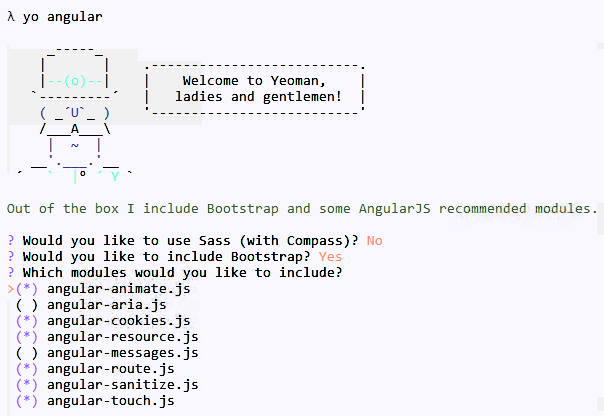
\includegraphics[width=.4\textwidth]{img/tp1_parte2/0-instalacionConYeoman}
  \caption{Confifuración inical de Yeoman}
  \label{yeomanInstall}
\end{figure}

Una vez terminada la configuración de Yeoman, en la carpeta del proyecto tendremos el esqueleto necesario para empezar a trabajar. En la  \textbf{Figura \ref{scaffold}} podemos ver cuales son los directorios principales, siendo estos \textbf{\textit{app}} donde se encuentran las imagenes, los controladores y las vistas y el directorio \textbf{\textit{test}} donde se encuentran los test respectivos para cada uno de los controladores.

\begin{figure}[h]
  \centering
  \includegraphics[width=.4\textwidth]{img/tp1_parte2/0-scaffold}
  \caption{Scaffold de la aplicación inicial.}
  \label{scaffold}
\end{figure}

\subsection{Diagrama de clases tentativo}
En la \textbf{Figura \ref{2-modelo_datos_general}} se presenta el diagrama de clases tentativo, dicho diagrama  será utilizado como base a lo largo de los futuros sprint a desarrollar y posee un alcance limitado el cual se irá modificando a medida que se profundice en los temas.

Para realizar este diagrama se utilizaron los user stories definidos con anterioridad y el relevamiento que se ha realizado hasta el momento, pero como se dijo anterirormente, muchos de los temas serán profundizados en cada Sprint.

\begin{sidewaysfigure}
  \centering
  \includegraphics[width=0.9 \textwidth]{img/tp1_parte2/0-DiagramaClasesGeneral}
  \caption{Modelo de datos General}
  \label{2-modelo_datos_general}
\end{sidewaysfigure}


\clearpage % Lo hice para que la imagen del scaffold no me quede tan abajo
\section{Sprint 1: Generación de perfil de datos personales}

\subsection{Descripción}
En este sprint se realizará la sección del perfil del usuario, para lo cual se deberá definir en el backend, las clases Profile y Gender, así como los recursos para acceder a ellas a través de la API. Además se realizara la documentación correspondiente para su consumo.
Por parte del frontend se debe desarrollar los recursos de acceso a la API, las vista HTML y cada uno de sus controladores: Una para mostrar el perfil y otra de edición del mismo.

Para lograr brindarle esta funcionalidad se desarrollarán los formularios de carga y edición para permitirle gestionar su información en el momento que lo desee.

\subsection{User Stories relacionados}
{\scriptsize
	\begin{table}[h]
		\begin{tabular}{|l|p{10cm}|c|}
			\hline
			\multicolumn{1}{|c|}{\textbf{ID}} &
			\multicolumn{1}{c|}{\textbf{Enunciado de la historia}} &
			\textbf{Prioridad} \\     
			\hline
			US-\ref{infoPerfil} &
			Como paciente quiero cargar mi información personal nombre, apellido, fecha de nacimiento y más para armar mi perfil e identificarme así en el sistema.& Alta
			\\
			\hline 
		\end{tabular}
	\end{table}
}




\subsection{Planificación}

\subsubsection{Período de realización}

\begin{itemize}
    \item \textbf{Inicio}: 28 de abril del 2015.
    \item \textbf{Fin}: 19 de mayo del 2015.
\end{itemize}

\subsubsection{Sprint Backlog}

{\scriptsize
	\begin{center} %sidewaystable
		\centering
		%\begin{adjustbox}{max width=\textheight}
		\resizebox{\textwidth}{!}{
			\begin{tabular}{|l|l|l|l|}
				\hline
				\textbf{Area a cargo} &
				\textbf{Responsable} &        
				\textbf{Tarea} &
				\textbf{US} \\
				\hline
				Front-end & Yanina Morales&  Generación de plantilla principal, con logo, botonera y colores  & US-\ref{resumenInfo} \\ \hline
				Front-end& Iván Terreno & Generación de controladores para consumir Json de la Api  & US-\ref{resumenInfo} \& US-\ref{infoSalud} \\ \hline
				Front-end& Iván Terreno & Capacitación sobre las ventajas de usar resource frente a http & US-\ref{resumenInfo} \& US-\ref{infoSalud}\\ \hline
				Front-end&Iván Terreno  & Creación de página de perfil&  US-\ref{resumenInfo}\\ \hline
				
				Back-end&Michael Manganiello  & Creación de aplicación  &  US-\ref{resumenInfo} \& US-\ref{infoSalud}\\ \hline
				Back-end&Michael Manganiello  & Exposición de métodos como servicios de API 	& US-\ref{resumenInfo} \& US-\ref{infoSalud}\\ \hline
				Back-end&Franco Canizo   & Adaptación de salida de métodos a formato Json&US-\ref{resumenInfo} \& US-\ref{infoSalud}\\ \hline
				Back-end&Franco Canizo  & Creación de base de datos inicial&US-\ref{resumenInfo} \& US-\ref{infoSalud}\\ \hline
			\end{tabular}
		}
		%\end{adjustbox}
	\end{center}
}


\subsection{Modelo Funcional}
En la \textbf{[Figura \ref{1-caso_de_uso}]} se representa el primer caso de uso a desarrollar por el sistema. El cual incluye funcionalidades inherentes, como dar de alta un nuevo perfíl, editarlo, y darlo de baja. También se incluye un menú de logueo aunque por su simplicidad se decidió no extraerlo de ``Gestionar Perfil'', ya que realmente es una corroboración de datos del usuario y puede ser visto como que se encuentra incluido.

\begin{figure}[h]
	\centering
	\includegraphics[width=0.6\textwidth]{img/tp1_parte2/1-caso_de_uso}
	\caption{formulario de edición de perfil}
	\label{1-caso_de_uso}
\end{figure}

Desde el punto de vista del backend se deben preparar los recursos POST para realizar inserciones,ediciones y el borrado de registros, a los cuales el usuario normal no puede tener acceso de ABM. Por eso el modelo funcional también incluye el caso de uso  ``Gestionar Genero'' representdo en \textbf{[Figura \ref{1-cu-admin}]}.


\begin{figure}[h]
	\centering
	\includegraphics[width=0.6\textwidth]{img/1-cu-admin}
	\caption{Casos de usos de Administración}
	\label{1-cu-admin}
\end{figure}



\subsection{Modelo de datos}

El Diagrama que propio de este sprint se puede ver en la \textbf{Figura \ref{modeloEspecifico}}, allí se indican exactamente las clases que se usarán en este sprint y que serán detalladas con detenimiento en el presente documento. Se recuerda que se ha realizado un Diagrama de clases tentativo que se puede ver en la \textbf{Figura \ref{2-modelo_datos_general}}, dicho diagrama  será utilizado como base para este sprint y posee un alcance limitado el cual se irá modificando a medida que se profundice en los temas.



\begin{figure}[h]
  \centering
  \includegraphics[width=0.3\textwidth]{img/tp1_parte2/1-modelo_dato_especifico}
  \caption{Modelo de datos Específico}
  \label{modeloEspecifico}
\end{figure}
\clearpage

A continuación se describen las clases que intervienen en el sprint.

    \subsubsection{Clase Profile}
    Dicha clase hace referencia a los datos que caracterizan al perfil del usuario.

    \textbf{Descripción de los atributos}
    \begin{itemize}
            \item \textbf{id:}Identificador único del perfil(tipo int)
			\item\textbf{ last\_name 	:}	Apellido de la persona(tipo string).
			\item \textbf{ first\_name: } 	Nombre de la persona (tipo string).
			\item \textbf{birthday 	:}	Fecha de nacimiento de la persona, en formato ISO 8601 (tipo datetime).
			\item \textbf{gender\_id:} 	Identificador único del género asociado 	(tipo int).
    \end{itemize} 
	\textbf{Dirección del recurso:}
    \begin{lstlisting}[language=json,firstnumber=1]
    <BASE URL>/profiles/{:id}
    \end{lstlisting}

    \textbf{Json generado por la API}    
    \begin{lstlisting}[language=json,firstnumber=1]
    {
    "resource": 
    {
    "id": 1,
    "gender": 
    {
    "id": 1,
    "name": "Masculino",
    "description": null
    },
    "birthday": "1990-10-26",
    "last_name": "Terreno",
    "first_name": "Milton"
    }
    }
    \end{lstlisting}

\subsubsection{Clase Gender} 
    \textbf{Descripción de los atributos}
	\begin{itemize}
            \item \textbf{name :}	Nombre del género (tipo string).
            \item \textbf{description 	:}	Descripción del género (tipo string).
    \end{itemize} 
    
    \textbf{Dirección del recurso:}
    \begin{lstlisting}[language=json,firstnumber=1]
    <BASE URL>/genders
    \end{lstlisting}

    \textbf{Json generado por la API}    
        \begin{lstlisting}[language=json,firstnumber=1]
{
    "resource": 
[
{
    "id": 1,
    "name": "Masculino",
    "description": null
},
        {
            "id": 2,
            "name": "Femenino",
            "description": null
        }
    ]
}
        \end{lstlisting}


	

    
\subsection {Salidas del Sistema - Incrementos}

Luego de finalizado este user story se obtendrá como salida el logo correspondiente a la aplicación que se muestra en la \textbf{Figura \ref{logoYesDoc}}, y 4 pantallas que se detallarán a continuación:
\begin{enumerate}
	\item \textbf{Logeo de usuario:} \textbf{[Figura \ref{logeo}]} Desde esta pantalla el usuario podrá logearse  o crear un perfil nuevo
	\item \textbf{Creación de perfil:}\textbf{[Figura \ref{crear_perfil}]} Se le permitirá cargar aquellos datos que lo identifique nombre, apellido, fecha de nacimiento y género.
    \item \textbf{Presentación de la información personal:} \textbf{[Figura \ref{perfil}]} Aquí se mostrarán los datos personales del usuario (nombre, apellido, fecha de nacimiento y género.), brindándole la posibilidad de edición de los mismos.
    \item \textbf{Edición del perfil:}\textbf{[Figura \ref{editar_perfil}]} En esta pantalla se mostrará el formulario para realizar la edición correspondiente del perfil, los campos estarán precargados con los valores del perfil del usuario, para que éste los modifique según disponga.
\end{enumerate}

\subsubsection{Actividades previas a las salidas del sistema}

\paragraph{Generación de plantilla principal, con logo, botonera y colores}

Se generará una plantilla que se utilizará en todas las distintas secciones de la web del proyecto. Esta plantilla incluye los colores principales de la aplicación, un logo representativo \textbf{Figura \ref{logoYesDoc}} y la funcionalidad que permite indicarle al usuario en que lugar esta situado (coloreo de botonera). 

\begin{figure}[h]
	\centering
	\includegraphics[width=0.1\textwidth]{img/tp1_parte2/2-logoYesDoc}
	\caption{Logo de la aplicación}
	\label{logoYesDoc}
\end{figure}

\paragraph{Capacitación sobre las ventajas de usar resource frente a http}

Se tuvo que realizar un análisis profundo sobre las ventajas que ofrece resource frente a http en el manejo de recursos brindados por la api, se decidió usar Resource porque proporciona una abstracción a un nivel por encima de \$http, es decir \$resource se vale internamente del objeto \$http y ya implementa CRUD como funciones básicas para persistencia. Al usar resource puede extenderse la base, el ejemplo más usado es modifficar el método update para que se ejecute la actualización por PUT. También trabaja internamente \$q (promises en angular), por tanto podemos usar promises siempre que hagamos una operación contra servidor.

\paragraph{Generación de controladores para consumir Json de la API}
Se generará el código necesario que permita obtener y hacer uso de los Json que genera la API, para esto es necesario crear un resource por cada controlador. En dicho resource se  hará uso de la API  a partir de la especificación de la respuesta brindada y los parámetros requeridos por la misma.


\paragraph{Creación de página de perfil}
En esta tarea  se generará la pantalla del perfil del usuario,\textbf{Figura \ref{perfil}} donde se mostrarán sus datos personales como son:
\begin{itemize}
	\item Nombre
	\item Apellido
	\item Fecha de nacimiento
	\item Género
\end{itemize}
Para poder presentar los datos del perfil al usuario será necesario  acceder al recurso \texttt{/profiles/\{:d\}} de la API a través de un método 		\textbf{GET}

\textbf{Especificaciones del recursos \texttt{/profiles}}

\begin{lstlisting}[language=json,firstnumber=1]
ProfileFields {
first_name (string),
last_name (string),
id (integer),
gender (GenderFields, optional),
birthday (date-time, optional)
}
GenderFields {
description (string, optional),
id (integer),
name (string)
} 
\end{lstlisting}

\textbf{Especificaciones del recursos \texttt{/genders}}
\begin{lstlisting}[language=json,firstnumber=1]
GenderFields {
description (string, optional),
id (integer),
name (string)
} 
\end{lstlisting}

Además se dará la posibilidad,al usuario, de acceder a la edición de su perfil desde la página de perfil. 


\begin{figure}[h]
	\centering
	\includegraphics[width=1\textwidth]{img/tp1_parte2/1-perfil}
	\caption{Pantalla de perfil de usuario}
	\label{perfil}
\end{figure}

\paragraph{Creación de página de formulario de creación de perfil}      
Se generará el formulario necesario para que el usuario pueda cargar los datos personales antes nombrados. Se presentará una pantalla provisoria de inicio \textbf{Figura \ref{logeo}}  donde se le dará lo opción de logearse o de generar un nuevo perfil.
La opción de \textbf{Nuevo Perfil}, conducirá al usuario al formulario \textbf{Figura \ref{crear_perfil}} donde se realizarán las cargas respectivas de datos
Para poder crear un nuevo perfil al usuario será necesario  acceder al recurso \texttt{/profiles/\{:d\}} de la API a través de un método \textbf{POST}
\begin{figure}[h]
	\centering
	\includegraphics[width=1\textwidth]{img/tp1_parte2/1-crear_perfil}
	\caption{Formulario de creación de perfil}
	\label{crear_perfil}
\end{figure}
\begin{figure}[h]
	\centering
	\includegraphics[width=1\textwidth]{img/tp1_parte2/1-logeo}
	\caption{Pantalla de logeo de usuario}
	\label{logeo}
\end{figure}

\paragraph{Creación de página de formulario de edición de perfil}      
\begin{figure}[h]
	\centering
	\includegraphics[width=1\textwidth]{img/tp1_parte2/1-editar_perfil}
	\caption{formulario de edición de perfil}
	\label{editar_perfil}
\end{figure}
Se generará el formulario necesario para que el usuario pueda modificar los datos personales antes nombrados. 
En la pantalla de perfil de usaurio \textbf{Figura \ref{perfil}} se le ofrecerá al usaurio la opción de \textbf{Editar Perfil} que lo redireccionará al formulario correspondiente a la edición del perfil, en los campos de dicho formulario se presentarán los datos del perfil, de este modo el usuario solo modificará el campo correspondiente
Para poder guardar los nuevos datos del perfil al usuario será necesario  acceder al recurso \texttt{/profiles/\{:id\}} de la API a través de un método \textbf{PUT}

\clearpage	
\subsection{Planificación de pruebas}
\subsubsection{Criterios de aceptación}


\begin{center}
\begin{longtable}{|m{0.5cm}|m{4cm}|m{4cm}|m{4.5cm}|}
\hline \rowcolor[gray]{0.9}
	\multicolumn{4}{|c|}{\textbf{Criterio de aceptación}} \\
    \hline  \rowcolor[gray]{0.9}
        \multicolumn{1}{|c|}{\textbf{ID}} &
        \multicolumn{1}{c|}{\textbf{Contexto}} &
        \multicolumn{1}{c|}{\textbf{Evento}} &
        \multicolumn{1}{c|}{\textbf{Resultado}} \\
    \hline
        1&En caso de que el usuario exista & y este quiera ingresar al sistema & El sistema le mostrara sus datos personales\\ \hline
        2 &       Si el usuario no existe & y quiere loguearse & El sistema no le permitirá ingresar\\ \hline
        3 &       Si el usuario existe y no está logueado & y quiere ingresar a ver su perfil& El sistema no le permitirá ingresar y lo mantendrá en la pantalla de login\\ \hline
        4 &       Si el usuario existe & y quiere editar su perfil & El sistema le permitirá modificar cualquiera de sus datos personales\\ \hline
  \end{longtable}
\end{center}


\subsubsection{Pruebas de unidad - Casos de Prueba}


	{\scriptsize
    \begin{table}[h]
    \centering
	\begin{tabular}{|m{4cm}|m{9cm}|}
    	\rowcolor[gray]{0.9}
	    \hline
       
		\textbf{Caso de prueba} & \textbf{Consultar perfil de usuario existente} \\  \hline
	    \textbf{Descripción del escenario}& Nombre: Marita; Apellido Martinez; fecha de Nacimiento:2015-06-01; género: femenino\\ \hline
	    \textbf{Criterio de aceptación}&  \textbf{En caso de que el usuario exista y este quiera ingresar al sistema. El sistema le mostrara sus datos personales}\\ \hline
        \textbf{Datos de entrada}&  Id:3\\ \hline
        \textbf{Condiciones de  prueba}& Se necesita que esté previamente cargado el usuario "Marita Martinez". \\ \hline
	\end{tabular}
        \caption{Caso de prueba para criterio de aceptación 1}
    \end{table}
	}
 
    	{\scriptsize
        \begin{table}[h]
        \centering
	\begin{longtable}{|m{4cm}|m{5cm}|m{4cm}|}
	    \hline  \rowcolor[gray]{0.9} 
        \multicolumn{3}{|c|}{\textbf{Procedimiento de Prueba - ``Consultar perfil de usuario existente''}} \\
        \hline \rowcolor[gray]{0.9}
	    \textbf{Actor} & \textbf{Sistema}&\textbf{Resultado Esperado} \\  \hline
	   El usuario ingresa en el campo login el id:3 & & \\ \hline
        &El Sistema realiza una consulta a la API a partir del id:3 solicitando los datos de la instancia perfil específica&   \\ \hline
        &&Se muestra el  perfil de usuario con sus datos: Nombre: Marita; Apellido Martinez; fecha de Nacimiento:2015-06-01; género: femenino  \\ \hline
	    \end{longtable}
        \caption{Procedimiento de prueba para criterio de aceptación 1}
        \end{table}
	}
    
    {\scriptsize
	\begin{table}[h]
	\centering
	\begin{tabular}{|m{3cm}|m{10cm}|}
	    \hline 
	    \textbf{Salida obtenida}&Se obtuvieron los datos que se detallaron previamente en ``Resultado esperado''\\ \hline
	    \textbf{Resultado}& \textbf{Correcto}\\ \hline
        \textbf{¿Qué fue mal?}& Nada\\ \hline      
        \textbf{Evidencia}&  \\ \hline
        \textbf{Seguimiento}& No es necesario ya que el caso de prueba no causó fallos \\ \hline
        \textbf{Estado}& \textbf{Terminado}\\ \hline        
        \textbf{¿Qué se puede mejorar?}& En una futura iteración se podría añadir el grupo sanguíneo y añadir un cartel de bienvenida al sistema \\ \hline              
	    \end{tabular}
        \caption{Resultado esperado para el criterio de aceptación 1}
    	\end{table}
	}
    

    %%%%%%%%   
    
\clearpage    
    
    {\scriptsize
	\begin{table}[h]
	\centering
	\begin{tabular}{|m{3cm}|m{10cm}|}
    	\rowcolor[gray]{0.9}
	    \hline 
	    \textbf{Caso de prueba} & \textbf{Consultar perfil de usuario No existente} \\  \hline
	    \textbf{Descripción del escenario}&\\ \hline
	    \textbf{Criterio de aceptación}&\textbf{Si el usuario no existe y quiere loguearse. El sistema no le permitirá ingresar}\\ \hline
        \textbf{Datos de entrada}&  Id:64\\ \hline
        \textbf{Condiciones de  prueba}& No existe un usuario con id=64 \\ \hline
	    \end{tabular}
        \caption{Caso de prueba para criterio de aceptación 2}
    	\end{table}
	}
    
    {\scriptsize
        \begin{table}[h]
        \centering
	\begin{longtable}{|m{4cm}|m{5cm}|m{4cm}|}
	    \hline \rowcolor[gray]{0.9} 
        \multicolumn{3}{|c|}{\textbf{Procedimiento de Prueba - ``Consultar perfil de usuario NO existente''}} \\
        \hline \rowcolor[gray]{0.9}
	    \textbf{Actor} & \textbf{Sistema}&\textbf{Resultado Esperado} \\  \hline
	   El usuario ingresa a loguearse con el id:64 & & \\ \hline
        & El Sistema realiza una consulta a la API a partir del id:64 solicitando los datos de la instancia perfil específica &   \\ \hline
        &El Sistema detecta que no existe un perfil con id:64&  Se mantiene al usuario en la vista de login\\ \hline
	    \end{longtable}
        \caption{Procedimiento de prueba para criterio de aceptación 2}
        
    	\end{table}
    }
    
    {\scriptsize
	\begin{table}[h]
	\centering
	\begin{longtable}{|m{3cm}|m{10cm}|}
	    \hline 
	    \textbf{Salida obtenida}&El sistema permitió el ingreso a la interfaz de perfil, mostrando los datos vacíos\\ \hline
	    \textbf{Resultado}& \textbf{Fallido} \\ \hline
        \textbf{¿Qué fue mal?}& El sistema no le debería haber permitido al usuario ingresar\\ \hline      
        \textbf{Evidencia}& Imagen \ref{prueba2} \\ \hline
        \textbf{Seguimiento}&  En la Imagen \ref{correccionprueba2} se pueden ver las modificaciones que tuvieron que hacerse en el código del archivo login.js del controller para poder resolver el error descubierto, las líneas en rojo son las que se encontraban en un comienzo, las cuales producían error, y tuvieron que ser reemplazadas por las lineas marcadas en verde para que las pruebas pasen. También se puede ver en las figura \ref{Codigoinicialprueba2} como se encontraba el código inicialmente.\\ \hline
        \textbf{Estado}& \textbf{Terminado \& Corregido}\\ \hline        
        \textbf{¿Qué se puede mejorar?}& Se corrigieron los errores pero en otra iteración se podría añadir carteles de advertencia, esto se verá en los sprint relacionados a la seguridad\\ \hline              
     
	    \end{longtable}
        \caption{Resultado esperado para el criterio de aceptación 2}
    	\end{table}
	}
    
\begin{figure}[h]
  \centering
  \includegraphics[width=1\textwidth]{img/tp1_parte2/1-prueba_2}
  \caption{Error en la prueba 2.}
  \label{prueba2}
\end{figure}

\begin{figure}[h]
  \centering
  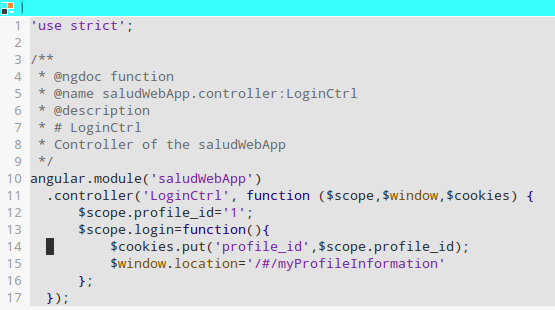
\includegraphics[width=1\textwidth]{img/tp1_parte2/1-codigo_prueba_2}
  \caption{Código utilizado inicialmente para el login.}
  \label{Codigoinicialprueba2}
\end{figure}


\begin{figure}[h]
  \centering
  \includegraphics[width=1\textwidth]{img/tp1_parte2/1-correccion_prueba_2}
  \caption{Correcciones de los errores detectados en la prueba 2.}
  \label{correccionprueba2}
\end{figure}

\clearpage
    %%%%%%%%%%%%%%%%%%%%%%

{\scriptsize
	\begin{table}[h]
	\centering
	\begin{tabular}{|m{3cm}|m{10cm}|}
    	\rowcolor[gray]{0.9}
	    \hline
	    \textbf{Caso de prueba} & \textbf{Ingresar al sistema sin loguearse} \\  \hline
	    \textbf{Descripción del escenario}& no son necesarios\\ \hline
	    \textbf{Criterio de aceptación}&\textbf{Si el usuario existe y no está logueado y quiere ingresar a ver su perfil, el sistema no le permitirá ingresar y lo mantendrá en la pantalla de login}\\ \hline
        \textbf{Datos de entrada}&  ninguno\\ \hline
        \textbf{Condiciones de  prueba}& el usuario no se loguea \\ \hline \hline
	    \end{tabular}
        \caption{Caso de prueba para criterio de aceptación 3}
    	\end{table}
	}
    
    {\scriptsize
	\begin{table}[h]
    \centering
	\begin{longtable}{|m{4cm}|m{5cm}|m{4cm}|}
	    \hline \rowcolor[gray]{0.9}
        \multicolumn{3}{|c|}{\textbf{Procedimiento de Prueba - ``Ingresar al sistema sin loguearse''}} \\
        \hline 
        \rowcolor[gray]{0.9}
	    \textbf{Actor} & \textbf{Sistema}& \textbf{Resultado Esperado} \\  \hline
	   El usuario selecciona la pestaña de ``perfil'' para ingresar a ver su perfil (sin antes haberse logueado) & & \\ \hline
        & El sistema valida que exista una cookie con las sesión creada&   \\ \hline
        &El Sistema no encuentra una cookie existente y no hace nada&  Se mantiene al usuario en la vista de login\\ \hline
	    \end{longtable}
        \caption{Procedimiento de prueba para criterio de aceptación 3}
    	\end{table}
    }
    
    {\scriptsize
	\begin{table}[h]
	\centering
	\begin{longtable}{|m{3cm}|m{10cm}|}
	    \hline 
	    \textbf{Salida obtenida}&El sistema mantuvo al usuario no logueado en la ventana de login, garantizando que no ingrese al sistema\\ \hline
	    \textbf{Resultado}& \textbf{Correcto}\\ \hline
        \textbf{¿Qué fue mal?}& Todo salio como se esperaba\\ \hline      
        \textbf{Evidencia}& Para esta prueba no es necesaria \\ \hline
        \textbf{Seguimiento}& No es necesario ya que el caso de prueba no causó
fallos \\ \hline
        \textbf{Estado}& \textbf{Terminado}\\ \hline        
        \textbf{¿Qué se puede mejorar?}& En otra iteración se podría añadir carteles de advertencia, esto se verá en los sprints relacionados a la seguridad.\\ \hline              
	    \end{longtable}
        \caption{Resultado esperado para el criterio de aceptación 3}
    	\end{table}
	}
    

\clearpage
    %%%%%%%%%%%%%%%%%%%%%%%%%%%%

    {\scriptsize
	\begin{table}[h]
	\centering
	\begin{tabular}{|m{3cm}|m{10cm}|}
    	\rowcolor[gray]{0.9}
	    \hline 
        \hline 
	    \textbf{Caso de prueba} & \textbf{Editar perfil} \\  \hline
	    \textbf{Descripción del escenario}&Nombre: Marita; Apellido Martinez; fecha de Nacimiento:2015-06-01; género: femenino; id:3\\ \hline
	    \textbf{Criterio de aceptación}& \textbf{Si el usuario existe y quiere editar su perfil, el sistema le permitirá modificar cualquiera de sus datos personales}\\ \hline
        \textbf{Datos de entrada }& datos modificados nombre: Marita Emilce\\ \hline
        \textbf{Condiciones de  prueba}&  usuario con id:3 logueado \\ \hline
	    \end{tabular}
        \caption{Caso de prueba para criterio de aceptación 4}
    	\end{table}
	}
    
    {\scriptsize
	\begin{table}[h]
    \centering
	\begin{longtable}{|m{4cm}|m{5cm}|m{4cm}|}
	    \hline \rowcolor[gray]{0.9}
        \multicolumn{3}{|c|}{\textbf{Procedimiento de Prueba - ``Editar perfil''}} \\
        \hline 
        \rowcolor[gray]{0.9}
	    \textbf{Actor} & \textbf{Sistema}& \textbf{Resultado Esperado} \\  \hline
	   El usuario presiona sobre el botón``editar perfil'' & & \\ \hline
        & El Sistema realiza una consulta a la API a partir del id:3 para traer los datos del perfil y precargar el formulario &   \\ \hline
        & &  Se muestra un formulario con los datos del usuario para que sean modificados\\ \hline
        El usuario modifica su nombre y añade un segundo nombre Emilce&& \\ \hline
        &El sistema carga los nuevos datos a la API a través del método PUT&\\ \hline
        &El sistema redirecciona al usuario a la vista de perfil de usuario&Se muestra el perfil con sus datos y el nuevo nombre ingresado\\ \hline
	    \end{longtable}
        \caption{Procedimiento de prueba para criterio de aceptación 4}
    	\end{table}
    }
    
    {\scriptsize
	\begin{table}[h]
	\centering
	\begin{tabular}{|m{3cm}|m{10cm}|}
	    \hline 
	    \textbf{Salida obtenida}& El formulario con los datos se mostraron correctamente\\ \hline
	    \textbf{Resultado}& \textbf{Correcto}\\ \hline
        \textbf{¿Qué fue mal?}& nada\\ \hline      
        \textbf{Evidencia}& En la Imagen \ref{prueba4} se puede ver el formulario con los datos precargados y en el Json \ref{JsonProfile} que contiene los nuevos datos los cuales accedemos a partir de la URL \begin{lstlisting} 
https://yesdoc-api.herokuapp.com/profiles/3 \end{lstlisting}\\ \hline
        \textbf{Seguimiento}& No es necesario ya que el caso de prueba no causó
fallos
\\ \hline
        \textbf{Estado}& \textbf{Terminado}\\ \hline        
        \textbf{¿Qué se puede mejorar?}& \\ \hline              
	    \end{tabular}
        \caption{Resultado esperado para el criterio de aceptación 4}
    	\end{table}
	}
\clearpage

\begin{figure}[h]
  \centering
  \includegraphics[width=1\textwidth]{img/tp1_parte2/1-prueba_4}
  \caption{Prueba 4}
  \label{prueba4}
\end{figure}

\begin{lstlisting}[language=json,firstnumber=1,  breaklines=true, caption= Json del perfil id:3 modificado, label=JsonProfile]
{
 "resource": {
    "gender":{
            "description": null,
            "id": 2,
            "name": "Femenino"
        },
        "first_name": "Marita Emilce",
        "last_name": "Martinez",
        "id": 3,
        "birthday": "2015-06-01"
    }
}
\end{lstlisting}

\clearpage
    %%%%%
    
    


    
    %%%%
    \clearpage
\subsubsection{Pruebas de integración entre módulos del Sistema}
Estas pruebas se realizarán más adelante, en futuros sprints.
\subsubsection{Pruebas de carga}
En este sprint no se realizarán este tipo de pruebas.
\subsubsection{Pruebas de seguridad por niveles de usuario}
En este sprint no se realizarán este tipo de pruebas, ya que la seguridad será un tema a tratar más adelante.

\subsection{Pruebas ejecutadas}
Aquí se realizará una conclusión general de lo que se descubrió en las pruebas.
	\begin{itemize}
		\item \textbf{¿Qué fue bien?}
        	\begin{itemize}
				\item Los datos de usuario se mostraron correctamente, además al cargar  los datos no se tuvo inconveniente alguno.
			\end{itemize}
   		\item \textbf{¿Qué se mejoró?}
        	\begin{itemize}
				\item \textbf{Cerrado}  Se detecto que cuando un usuario inexistente iniciaba sesión, podía ingresar al módulo de perfil, en este módulo no se mostraban los datos, ya que no existía  el usuario, pero no era correcto que esto sucediera.
                \item \textbf{Cerrado} Se encontraron problemas  con los nav's, los cuales sólo se marcaban como seleccionados cuando se presionaban y esto no nos servía para los casos en los que había que redireccionar. Se solucionó utilizando Angular Strap.
                
			\end{itemize}
   		\item \textbf{¿Qué se puede mejorar?}
        	\begin{itemize}
				\item \textbf{Abierto} Al finalizar el Sprint se vio necesario implementar un ítem que indique el grupo sanguíneo de la persona.
                \item \textbf{Abierto} Se podría arreglar la forma de seleccionar las fechas en el caso de la "fecha de nacimiento".
                \item \textbf{Abierto} Se deberá añadir, en los sprint relacionados a seguridad, los carteles de advertencia correspondientes.
                \item \textbf{Abierto} En próximas iteraciones deberá añadirse el grupo sanguíneo de la persona
                \item \textbf{Abierto} En próximas iteraciones deberá añadirse un cartel de bienvenida del usuario al sistema.
			\end{itemize}
    \end{itemize}
\section{Sprint 2: Creación y gestión de mediciones} %CREAR, EDITAR Y MOSTRAR MEDICIONES


\subsection{Descripción}
En este sprint se llevarán a cabo las interfaces necesarias para que el usuario pueda cargar nuevas mediciones y ver todas sus últimas mediciones ,así teniendo un seguimiento de las mismas con posibilidad de que posteriormente pueda ver su evolución a través de gráficas y tablas.
Para la comunicación de estas interfaces con la API, se desarrollarán los correspondientes adaptadores para los recursos.

Para esto en el backend se deben preparar las clases Measurement, MeasurementType,MeasurementSource,MeasurementUnit con las debidas relaciones con las clase Profile desarrollada en el sprint anterior.
Para cada una de esas clases, se deben preparar interfaces de acceso a los recursos provistos por la API. Y su correspondiente documentación.


\subsection{User Stories relacionados}
La \textbf{Tabla \ref{US-Sprint2}} indicará las características de cada user story para guiarnos en el desarrollo del sprint.

\begin{table}[h]
	%\resizebox{\textwidth}{!}{
    \centering
	\begin{tabular}{|l|p{9cm}|c|}
	\hline
        \multicolumn{1}{|c|}{\textbf{ID}} &
        \multicolumn{1}{|c|}{\textbf{Enunciado de la historia}} &
        \textbf{Prioridad} \\          
    \hline
        US-\ref{resumenInfo} &
        Como paciente quiero obtener un resumen de mi información de salud básica para hacer uso de la misma en caso de una emergencia &Alta
        \\
    \hline 
	    US-\ref{infoSalud} &
        Como paciente quiero cargar mi información personal de salud referido a mediciones (altura, grasa corporal, peso, presión arterial), para que el médico cuente con más y mejor información al momento de realizar el diagnóstico. & Alta
        \\
    \hline
    \end{tabular}
%     }
    \caption{Listado de \textit{User Stories} relacionados.}
    \label{US-Sprint2}
\end{table}

\subsection{Planificación}

\subsubsection{Período de realización}

\begin{itemize}
    \item \textbf{Inicio}: 19 de mayo del 2015.
    \item \textbf{Fin}: 1 de julio del 2015.
\end{itemize}

\subsubsection{Sprint Backlog}

{\scriptsize
	\begin{center} %sidewaystable
		\centering
		%\begin{adjustbox}{max width=\textheight}
		\resizebox{\textwidth}{!}{
			\begin{tabular}{|l|l|l|p{5cm}|l|p{1cm}|}
				\hline
				\textbf{Área a cargo} &
				\textbf{Responsable} &        
				\textbf{Revisor} &        	        
				\textbf{Tarea} &
				\textbf{US} &
				\textbf{Tiempo dedicado} \\
				\hline
				Documentación& Yanina Morales & & Trabajo práctico nº 2 y avance de etapa de diseño &  & 20 horas \\ \hline        
				Documentación& Iván Terreno & & Trabajo práctico nº2 y avance de etapa de diseño  &  & 20 horas \\ \hline        
				Documentación& Michael Manganiello& & Trabajo práctico nº 2 y avance de etapa de diseño  &  & 20 horas \\ \hline        
				Documentación& Franco Canizo & & Trabajo práctico nº 2 y avance de etapa de diseño  &  & 20 horas \\ \hline         
				Front-end & Michael Manganiello& -- & Despliegue de la aplicación en Heroku  & US-\ref{resumenInfo} \& US-\ref{infoSalud}& 4 horas  \\ \hline     
				Capacitación & Yanina Morales& & Capacitación en utilización de Angular de manera desacoplada & US-\ref{infoSalud} & 12 horas \\ \hline        
				Capacitación & Iván Terreno& & Capacitación en utilización de Angular de manera desacoplada& US-\ref{infoSalud} & 12 horas\\ \hline                
				Front-end& Iván Terreno & Michael Manganiello & Generación de controladores para consumir Json de la Api relacionados a la API & US-\ref{resumenInfo} \& US-\ref{infoSalud}& 8 horas  \\ \hline
				Front-end & Yanina Morales& Michael Manganiello & Creación de página de formulario de carga de mediciones& US-\ref{infoSalud} & 4 horas \\ \hline
				Front-end & Iván Terreno  & Michael Manganiello & Creación de página de formulario de carga de perfil& US-\ref{infoSalud} & 4 horas \\ \hline
				Front-end & Iván Terreno  & Michael Manganiello & Realización de pruebas& & 8 horas \\ \hline        
				Front-end & Yanina Morales  & Iván Terreno  & Realización de pruebas & & 12 horas \\ \hline         
				
				Back-end & Michael Manganiello & Franco Canizo & Creación de modulo de mediciones&US-\ref{resumenInfo} \& US-\ref{infoSalud} & 8 horas \\ \hline
				Back-end & Michael Manganiello & Iván Terreno & Exposición de métodos como servicios de API 	& US-\ref{resumenInfo} \& US-\ref{infoSalud} & 8 horas \\ \hline
				Back-end & Franco Canizo & Michael Manganiello   & Adaptación de salida de métodos a formato Json&US-\ref{resumenInfo} \& US-\ref{infoSalud} & 8 horas \\ \hline
				Back-end & Franco Canizo & Michael Manganiello  & Carga de valores a la base de datos, relacionados a la API&US-\ref{resumenInfo} \& US-\ref{infoSalud} & 8 horas \\ \hline
			\end{tabular}
		}
		%\end{adjustbox}
	\end{center}
}

\subsubsection{Actividades de integración}

\begin{figure}[h]
  \centering
  \includegraphics[width=1\textwidth]{img/2-PR}
  \caption{Pull requests realizados por el front-end.}
  \label{2-PR}
\end{figure}
\begin{figure}[h]
  \centering
  \includegraphics[width=1\textwidth]{img/2-PR_back2}
  \caption{Pull requests realizados por el back-end, primera parte.}
  \label{2-PR_back2}
\end{figure}
\begin{figure}[h]
  \centering
  \includegraphics[width=1\textwidth]{img/2-PR_Back}
  \caption{Pull requests realizados por el back-end, segunda parte.}
  \label{2-PR_Back}
\end{figure}

\clearpage
    
	


\begin{comment}
\subsection{Fase de Análisis}

En esta fase comenzaremos definiendo el Sprint backlog y describiendo en detalle cada una de las tareas que la componen, además se realizará un diagrama de clases iniciales (\textbf{Figura \ref{modelo_datos}}) que nos permitirá guiarnos durante el avance del sprint de ese modo obtener un sistema consistente. 
\end{comment}


\subsection{Modelo funcional} %Diagrama de clases

En la \textbf{[Figura \ref{2-caso_de_uso}]} podemos observar el caso de uso representativo de las funcionalidades a adiquirir en este sprint.
El mismo representa a Agregar una nueva medición, editar mediciones existentes y eliminar mediciones.

\begin{figure}[h]
	\centering
	\includegraphics[width=0.5\textwidth]{img/2-caso_de_uso}
	\caption{formulario de edición de perfil}
	\label{2-caso_de_uso}
\end{figure}

Desde el punto de vista del backend se deben preparar los recursos POST para realizar inserciones,ediciones y el borrado de registros, a los cuales el usuario normal no puede tener acceso de ABM. Por eso el modelo funcional también incluye los casos de uso ``Gestionar Tipo de Medición'',``Gestionar Unidad de Medición'' y ``Gestionar Fuente de Medición'' representados en \textbf{[Figura \ref{2-cu-admin}]}.

\begin{figure}[h]
	\centering
	\includegraphics[width=0.6\textwidth]{img/2-cu-admin}
	\caption{Casos de usos de Administración}
	\label{2-cu-admin}
\end{figure}

\subsection{Modelo de datos}
El Diagrama propio de este sprint se puede ver en la \textbf{Figura \ref{sp2_modelo_especifico}}, allí se indican exactamente las clases que se usarán en este sprint y que serán detalladas con detenimiento en el presente documento. Se recuerda que se ha realizado un Diagrama de clases tentativo que se puede ver en la \textbf{Figura \ref{2-modelo_datos_general}}, dicho diagrama  será utilizado como base para este sprint y posee un alcance limitado el cual se irá modificando a medida que se profundice en los temas.



\begin{figure}[h]
  \centering
  \includegraphics[width=1\textwidth]{img/2-DC_especifico}
  \caption{Modelo de datos}
  \label{sp2_modelo_especifico}
\end{figure}
\clearpage

A continuación se describen las clases que intervienen en el sprint.

\subsubsection{Clase Measurement} 
Dicha clase se refiere a las medición realizada por el usuario en un momento específico. 

\textbf{Descripción de los atributos}
	\begin{itemize}
		\item \textbf{id:} Identificador único de la medición (tipo int).
        \item \textbf{datetime:} Fecha y hora de la medición (tipo datetime).
        \item \textbf{value:} Valor de la medición (tipo float).
        \item \textbf{profile\_id:} Identificador único del perfil asociado (tipo int).
        \item \textbf{measurement\_source\_id:}Identificador único de la fuente de medición asociada (tipo int).
        \item \textbf{measurement\_type\_id:}Identificador único del tipo de medición asociado (tipo int).
        \item \textbf{measurement\_unit\_id:}Identificador único de la unidad de medición asociada (tipo int).
        
	\end{itemize}
    
\textbf{Dirección del recurso:}
\begin{lstlisting}[language=json,firstnumber=1]
<BASE URL>/measurements/{:id}
\end{lstlisting}

\textbf{Json generado por la API}    
\begin{lstlisting}[language=json,firstnumber=1]
{
    "resource": 
{
    "measurement_unit": 
{
    "symbol": "Kg",
    "suffix": true,
    "name": "Kilogramo",
    "id": 1
},
"measurement_source": 
{
    "name": "Manual",
    "description": null,
    "id": 1
},
"value": 50,
"measurement_type": 
{
    "name": "Peso",
    "description": "Peso corporal de la persona.",
    "id": 1
},
"id": 1,
"profile": 
{
    "birthday": "1990-10-26",
    "last_name": "Terreno",
    "first_name": "Milton",
    "gender": 
            {
                "name": "Masculino",
                "description": null,
                "id": 1
            },
            "id": 1
        },
        "datetime": "2015-06-15T02:29:54"
    }
}
\end{lstlisting}
\subsubsection{Clase MeasurementType}
Esta clase nos permitirá  nomenclar  los tipos de medidas, hasta el momento hemos contemplado: peso, dimensión corporal (Ej:altura) y glucosa. Existen ciertas medidas que contemplan dos valores, estas serán agregadas en un sprint futuro.

\textbf{Descripción de los atributos}
    \begin{itemize}
			\item \textbf{name: }	Nombre del tipo de medición(tipo string).
            \item \textbf{description:} Descripción del tipo de medición (tipo string).
    \end{itemize}

\textbf{Dirección del recurso:}
\begin{lstlisting}[language=json,firstnumber=1]
<BASE URL>/measurement_types/{id}
\end{lstlisting}

\textbf{Json generado por la API} 
\begin{lstlisting}[language=json,firstnumber=1]
{
    "resource": 
    {
        "name": "Peso",
        "description": "Peso corporal de la persona.",
        "id": 1
    }
}
\end{lstlisting}

\subsubsection{Clase MeasurementUnit}
Esta clase nos permitirá  nomenclar  las unidades de medición disponible para que el usuario pueda seleccionarlas cuando realice la medición, hasta el momento hemos contemplado: Kilogramo, gramo, miligramos, metro, centímetro y milímetro.

    \textbf{Descripción de los atributos}
        \begin{itemize}
            \item \textbf{id:	}	Identificador único de la unidad de medición(tipo int).
            \item \textbf{name :	}	Nombre de la unidad de medición ( tipo string).
            \item \textbf{symbol :}		Símbolo de la unidad de medición (tipo string).
            \item \textbf{suffix :}	Variable booleana que indica si el símbolo de la unidad de medición es un sufijo (verdadero) o un prefijo (falso) del valor de la medición (tipo boolean).
        \end{itemize}

    \textbf{Dirección del recurso}
        \begin{lstlisting}[language=json,firstnumber=1]
        <BASE URL>/measurement_units/{id}
        \end{lstlisting}

    \textbf{Json generado por la API} 
        \begin{lstlisting}[language=json,firstnumber=1]
        {
            "resource": 
            {
                "symbol": "Kg",
                "suffix": true,
                "name": "Kilogramo",
                "id": 1
            }
        }
        \end{lstlisting}

\subsubsection{Clase MeasurementSource}
Esta clase nos permitirá nomenclar los tipos de fuentes posibles como pueden ser manual, dispositivo móvil, sistema de salud y dispositivo de salud.
    
	\textbf{Descripción de los atributos}
        \begin{itemize}
            \item \textbf{name 	:}	Nombre de la fuente de medición (tipo string).
            \item \textbf{description 	:}	Descripción de la fuente de medición (tipo String).
        \end{itemize}
    \textbf{Dirección del recurso}
    \begin{lstlisting}[language=json,firstnumber=1]
    <BASE URL>/measurement_sources/{:id}
    \end{lstlisting}

    \textbf{Json generado por la API} 
    \begin{lstlisting}[language=json,firstnumber=1]
{
    "resource": 
    {
        "name": "Manual",
        "description": null,
        "id": 1
    }
}
    \end{lstlisting}
    
\clearpage
\newpage

\subsection {Salidas del Sistema - Incrementos}

Luego de finalizado este user story se obtendrán 4 pantallas que se detallarán a continuación:
\begin{enumerate}
    \item \textbf{Presentación de las últimas mediciones}  \textbf{[Figura  \ref{perfil_medicion}]} con posibilidad de edición de cada una de las mediciones. Los datos posible  a presentar son altura, peso, grasa corporal y glucosa. 
    
    La interfaz mostrará el valor de la medición, la fecha y hora en que fue realizada y la fuente que se utilizó para dicha medición.
	\item \textbf{Carga de mediciones}: \textbf{[Figura \ref{nueva_medicion}]} Se le permitirá cargar mediciones que realice en algún momento del día como son peso, altura, grasa corporal y glucosa. Deberá indicar la fuente, tipo, unidad y fecha de la medición
    \item \textbf{Edición de mediciones:}  \textbf{[Figura \ref{editar_medicion}]} Se le permitirá seleccionar una medición del perfil de mediciones para sel modificada.

\end{enumerate}

\clearpage
\subsubsection{Actividades previas a las salidas del sistema}

\paragraph{Creación de página de mediciones}
En esta tarea  se generará la pantalla, \textbf{Figura \ref{perfil_medicion}} donde se muestran las mediciones del usuario, como lo son:
\begin{itemize}
	\item Altura
	\item Peso
	\item Grasa Corporal
	\item Presión Arterial
\end{itemize}
Al igual que en la creación del perfil se dará la posibilidad de acceder a la edición de su perfil desde esta misma página.

\begin{sloppypar}
Para mostrarlas mediciones del usuario es necesario acceder al recurso \texttt{/profiles/\{profile\_id\}/measurements/latest} de la API a través de un método \textbf{GET}
\end{sloppypar}


\textbf{Especificaciones del recursos \texttt{/measurements}}

\begin{lstlisting}[language=json,firstnumber=1]
MeasurementFields {
measurement_source (MeasurementSourceFields, optional),
profile (ProfileFields),
datetime (date-time),
value (number),
measurement_unit (MeasurementUnitFields),
id (integer),
measurement_type (MeasurementTypeFields)
}
MeasurementSourceFields {
description (string, optional),
id (integer),
name (string)
}
ProfileFields {
first_name (string),
last_name (string),
id (integer),
gender (GenderFields, optional),
birthday (date-time, optional)
}
GenderFields {
description (string, optional),
id (integer),
name (string)
}
MeasurementUnitFields {
id (integer),
symbol (string),
suffix (boolean, optional),
name (string)
}
MeasurementTypeFields {
description (string, optional),
id (integer),
name (string)
} 
\end{lstlisting}

En el perfil de usuario se mostrarán de cada tipo de medición que ha realizado el usuario la última de cada una, indicando el nombre, el valor, el símbolo, la fecha y hora y el método con el que ha sido realizada la medición. Además para cada una de las mediciones se mostrarán dos iconos que corresponden a la edición y a la compartición de las mediciones, este último será implementado en un sprint futuro.

\begin{figure}[h]
	\centering
	\includegraphics[width=1\textwidth]{img/2-perfil_medicion}
	\caption{Perfil de mediciones}
	\label{perfil_medicion}
\end{figure}

\clearpage
\paragraph{Creación de página de formulario de carga de mediciones}
Se generará el formulario necesario, que se muestra en la \textbf{Figura \ref{nueva_medicion}} para que el usuario pueda cargar las mediciones antes nombrados, para ello es necesario acceder al recurso \texttt{/measurements} de la API a través de un método \textbf{POST}

\begin{lstlisting}[language=json,firstnumber=1]
MeasurementFields {
measurement_source (MeasurementSourceFields, optional),
profile (ProfileFields),
datetime (date-time),
value (number),
measurement_unit (MeasurementUnitFields),
id (integer),
measurement_type (MeasurementTypeFields)
}
MeasurementSourceFields {
description (string, optional),
id (integer),
name (string)
}
ProfileFields {
first_name (string),
last_name (string),
id (integer),
gender (GenderFields, optional),
birthday (date-time, optional)
}
GenderFields {
description (string, optional),
id (integer),
name (string)
}
MeasurementUnitFields {
id (integer),
symbol (string),
suffix (boolean, optional),
name (string)
}
MeasurementTypeFields {
description (string, optional),
id (integer),
name (string)
} 
\end{lstlisting}

Desde el perfil de mediciones se presentará un icono que representa a la creación de un elemento para que el usuario pueda seleccionarlo. Esta acción llevara al usuario al formulario de creación de mediciones, donde los campos estarán vacíos, para que el usuario los cargue con los valores correspondientes. Una vez terminada la carga, se mostrará un mensaje avisando al usuario que se ha realizado con éxito y luego lo direccionará al perfil de mediciones.

\begin{figure}[h]
	\centering
	\includegraphics[width=1\textwidth]{img/2-nueva_medicion}
	\caption{Formulario de nueva medición}
	\label{nueva_medicion}
\end{figure}

\clearpage
\paragraph{Creación de página de formulario de edición de mediciones}
Se generará el formulario necesario, que se muestra en la \textbf{Figura \ref{editar_medicion}} para que el usuario pueda editar una medición previamente seleccionada, para ello es necesario acceder al recurso \texttt{/measurements/\{:id\}} a través del método \textbf{PUT} enviando por URL el id correspondiente a dicha medición. 

Desde el perfil de mediciones se presentará un icono que representa a la edición de un elemento para que el usuario pueda seleccionarlo. Esta acción llevara al usuario al formulario de edición de mediciones, donde los campos estarán cargados con los valores antiguos, de este modo el usuario modifica lo que desea y no tiene que cargar todo nuevamente. Una vez terminada la edición se direccionará al perfil de mediciones.

\begin{figure}[h]
	\centering
	\includegraphics[width=1\textwidth]{img/2-editar_medicion}
	\caption{Formulario de edición de medición}
	\label{editar_medicion}
\end{figure}




%%%%%%%%%%%%%%%%%%%%%% COMPLETAR!!! %%%%%%%%%%%%%%%%%%%%%%%%%%%%
\begin{comment}


\subsubsection{Creación de aplicación  }
\subsubsection{Creación de modulo de mediciones}
\subsubsection{Exposición de métodos como servicios de API}
\subsubsection{Adaptación de salida de métodos a formato Json}
\subsubsection{Creación de base de datos inicial}
\end{comment}


\clearpage
\subsection{Planificación de pruebas}
\subsubsection{Criterios de aceptación}

\begin{center}
\begin{longtable}{|p{0.5cm}|p{4cm}|p{4cm}|p{4.5cm}|}
\hline \hline \rowcolor[gray]{0.9}
	\multicolumn{4}{|c|}{\textbf{Criterio de aceptación}} \\
    \hline  \rowcolor[gray]{0.9}
        \textbf{Id} &
        \textbf{Contexto} &
        \textbf{Evento}&
        \textbf{Resultado} \\
    \hline
1&En caso de que exista una persona sin mediciones & cuando este desee observar sus mediciones  & El sistema no mostrará nada \\ \hline
 
2& Cuando el usuario registrado ingresa dos mediciones del mismo tipo  & y luego quiera consultarlas & El sistema solo le mostrará la ultima medición, del mismo tipo, realizada\\ \hline

3& Cuando el usuario seleccione una medición & y luego quiera editarla & El sistema le permitirá la correspondiente edición\\ \hline

4& Si el usuario existe y no está logueado & y quiera ingresar a ver sus mediciones. & El sistema no le permitirá ingresar\\ \hline
  \end{longtable}
\end{center}

\clearpage
\subsubsection{Casos de Prueba}


	\begin{table}
	\centering
	\begin{tabular}{|m{4cm}|m{9cm}|}
    	\rowcolor[gray]{0.9}
        \hline 
	    \textbf{Caso de prueba} & \textbf{Consultar mediciones (sin medidas precargadas)}\\  \hline
	    \textbf{Descripción del escenario}& Nombre: Marita; Apellido Martinez; fecha de Nacimiento:20-08-1989; id:3  \\ \hline
	    \textbf{Criterio de aceptación}&  \textbf{En caso de que exista una persona sin mediciones cargadas, si el usuario desea verlas el sistema no debería mostrar ninguna medición.} \\ \hline
        \textbf{Datos de entrada}&  consultar mediciones\\ \hline
        \textbf{Condiciones de  prueba}& Se necesita que esté previamente cargado el usuario ``Marita Martinez'' y no tenga datos más allá de su nombre y apellido en el perfil \\ \hline
	    \end{tabular}
        \caption{Caso de prueba para criterio de aceptación 1}
    	\end{table}
  
{\scriptsize
	\begin{table}[h]
    \centering
	\begin{longtable}{|p{5cm}|p{5cm}|p{5cm}|}
	    \hline \hline \rowcolor[gray]{0.9}
        \multicolumn{3}{|c|}{\textbf{Procedimiento de Prueba - ``Consultar mediciones''}} \\
        \hline \rowcolor[gray]{0.9}
		    \textbf{Actor} & 
	        \textbf{Sistema}& 
        	\textbf{Resultado esperado} \\  
        \hline
	    El usuario ingresa al sistema con su id nº3	& &\\ \hline
        		& El sistema valida con los perfiles de la API si el Id:3 del usuario existe& Se presenta por pantalla el perfil del usuario con sus datos  \\ \hline        
	    El usuario selecciona la pestaña mediciones y realiza la consulta& &\\ \hline
      	&El sistema valida que las cookies estén activas&\\ \hline
   		&El sistema solicita a la API las mediciones del perfil con id:3&El sistema no muestra ninguna medida cargada \\ \hline 
	    \end{longtable}
		\caption{Procedimiento de prueba para criterio de aceptación 1}
    	\end{table}
	}
    
        {\scriptsize
	\begin{table}[h]
	\centering
	\begin{tabular}{|l|p{10cm}|}
	    \hline 
	    \textbf{Salida obtenida}& No se presentan datos de mediciones\\ \hline
	    \textbf{Resultado}& \textbf{Correcto}\\ \hline
        \textbf{¿Qué fue mal?}& Nada\\ \hline      
        \textbf{Evidencia}& \\ \hline
        \textbf{Seguimiento}&No es necesario ya que el caso de prueba no causó
fallos \\ \hline
        \textbf{Estado}& \textbf{Terminado}\\ \hline        
         \textbf{¿Qué se puede mejorar?}& En otra iteración se debería añadir carteles de avisos, informando que faltan cargar datos \\ \hline              
	    \end{tabular}
        \caption{Resultado esperado para el criterio de aceptación 1}
    	\end{table}
	}
\clearpage 
%%%%%%%%%%%%%%%%%%%%%%%%%%%%%%%%%%%%%%%%%%%%%%%%%%

{\scriptsize
	\begin{table}[h]
	\centering
	\begin{tabular}{|m{4cm}|m{9cm}|}
    	\rowcolor[gray]{0.9}
	    \hline
	    \textbf{Caso de prueba}  &  \textbf{Consultar mediciones (medida precargada)}\\  \hline
	    \textbf{Descripción del escenario}& Nombre: Marita; Apellido Martinez; fecha de Nacimiento:20-08-1989; id:3; altura: 2m  \\ 			\hline
	    \textbf{Criterio de aceptación} &\textbf{Cuando el usuario registrado ingresa dos mediciones del mismo tipo y luego quiera consultarlas. El sistema solo le mostrará la ultima medición, del mismo tipo, realizada} \\ \hline
        \textbf{Datos de entrada}& id:3; Peso 1: 67kg; peso 2: 55kg \\ \hline
        \textbf{Condiciones de  prueba}& el usuario Marita Martinez existe \\ \hline
	    \end{tabular}
        \caption{Caso de prueba para criterio de aceptación 2}        
	    \end{table}
}
 
   %{\scriptsize
	\begin{longtable}{|m{4cm}|m{5cm}|m{4cm}|}
 
	    \hline \hline \rowcolor[gray]{0.9}
        \multicolumn{3}{|c|}{\textbf{Procedimiento de Prueba - Consultar mediciones}} \\ \hline
	    \hline 
        \rowcolor[gray]{0.9}
	    \textbf{Actor} & \textbf{Sistema}& \textbf{Resultado Esperado} \\  \hline
	    El usuario se logea en el sistema& & \\ \hline
        & El sistema consulta la API para corroborar que el perfil con id:3 existe &\\ \hline
        &  El sistema redirecciona al usuario a la vista de perfil de usuario&Se muestra el perfil de usuario con los datos respectivos\\ \hline
	    El usuario selecciona la pestaña de mediciones de la barra de navegación& &\\ \hline
        & El sistema verifica las cookies del usuario para determinar si ya se encuentra logeado &\\ \hline
        & El sistema redirecciona al usuario a la vista de mediciones&Se muestra la vista de mediciones con las últimas mediciones del usuario correspondientes\\ \hline  
        El usuario selecciona el botón de añadir ``nueva medicion''& &\\ \hline       
        & El sistema verifica que las cookies posean los datos del usuario&\\ \hline       
        & Se redirecciona a la vista de carga de mediciones&Se presenta el formulario de medición para la carga respectiva\\ \hline
        El usuario selecciona: Tipo de medicion: Peso; medida 55; unidad: Kg; Fuente: manual; fecha: deja la precargada y  luego de esto presiona el botón save& &\\ \hline       
        & El sistema valida que estén todos los datos cargado, excepto fuente el cual no es necesario, carga los nuevos datos en la API a través del método POST y redirecciona a la vista de mediciones&\\ \hline       
        &El sistema a través del método GET trae las últimas mediciones. &Se muestran las últimas mediciones en la vista de mediciones\\ \hline
        El usuario presiona el botón ´´cargar mediciones'' nuevamente& &\\ \hline  
        & El sistema verifica que las cookies posean los datos del usuario&\\ \hline       
        & Se redirecciona a la vista de carga de mediciones&Se presenta el formulario de mediciones para la carga respectiva\\ \hline
        El usuario selecciona: Tipo de medicion: Peso; medida 67; unidad: Kg; Fuente: manual; fecha: deja la precargada y  luego de esto presiona el botón save& &\\ \hline       
        & El sistema valida que estén todos los datos cargado, excepto fuente el cual no es necesario, carga los nuevos datos en la API a través del método POST y redirecciona a la vista de mediciones&\\ \hline       
        &El sistema a través del método GET trae las últimas mediciones. &El sistema muestra la última medición cargada ``Peso 55 Kg, fecha de carga y método: manual\\ \hline
        \caption{Procedimiento de prueba para criterio de aceptación 2}
        
	    \end{longtable}
        
	%}
\clearpage

{\scriptsize
	\begin{table}[h]
	\centering
	\begin{tabular}{|m{3cm}|m{10cm}|}
	    \hline 
	    \textbf{Salida obtenida}& Se mostraron correctamente la ultima medición del mismo tipo\\ \hline
	    \textbf{Resultado}& \textbf{Correcto}\\ \hline
        \textbf{¿Qué fue mal?}& Nada\\ \hline      
        \textbf{Evidencia}& En Listing \ref{JsonMediciones} se puede observar que el usuario posee 3 mediciones, dos de las cuales son del mismo tipo (tipo Peso) y en la Figura \ref{perfil_id_3} se puede ver que solo se muestra la última medición del Peso.  \\ \hline
        \textbf{Seguimiento}& no es necesario\\ \hline
        \textbf{Estado}& \textbf{Terminado}\\ \hline        
        \textbf{¿Qué se puede mejorar?}& \\ \hline              
	    \end{tabular}
        \caption{Resultado esperado para el criterio de aceptación 2}
    	\end{table}
	}


{\scriptsize
%\begin{minipage}{1 \textwidth}
    \begin{lstlisting}[language=json,firstnumber=1,  breaklines=true, caption= Json de las mediciones del perfil id:3, label=JsonMediciones]

        {"resource": 
	        [{
	    	    "measurement_source": 
        		{
		            "id": 1,
        		    "description": null,
		            "name": "Manual"
        		},
		        "measurement_type": 
        		{
		            "id": 1,
		            "description": "Peso corporal de la persona.",
		            "name": "Peso"
		        },
        		"datetime": "2015-07-03T11:51:39.436000",
		        "value": 55,
		        "id": 16,
    	    	"measurement_unit": 
                {
             	   "id": 1,
	               "suffix": true,
	               "name": "Kilogramo",
	               "symbol": "Kg"
	             }
    	    },
        	{
            	"measurement_source": 
		        {
        		    "id": 1,
		            "description": null,
		            "name": "Manual"
		        },
	        	"measurement_type": 
    		    {
	        	    "id": 1,
		            "description": "Peso corporal de la persona.",
		            "name": "Peso"
		        },
        		"datetime": "2015-07-03T11:54:22.806000",
		        "value": 67,
		        "id": 17,
        	"measurement_unit": 
	            {
    	            "id": 1,
        	        "suffix": true,
            	    "name": "Kilogramo",
                	"symbol": "Kg"
                }
              },
              {"measurement_source": 
                {
                    "id": 0,
                    "description": null,
                    "name": null
                },
               "measurement_type": 
                {
                    "id": 2,
                    "description": "Longitud de la persona",
                    "name": "Altura"
                },
	                "datetime": "2015-07-03T13:05:57.375000",
    	            "value": 2,
        	        "id": 18,
                "measurement_unit": 
                    {
                        "id": 2,
                        "suffix": true,
                        "name": "Metros",
                        "symbol": "m"
                    }
    	    }]
        }   
    \end{lstlisting}   


\begin{figure}[h]
        \centering
        \includegraphics[width=1\textwidth]{img/2-prueba_2}
        \caption{Perfil de medición de usuario con id:3}
		\label{perfil_id_3}
\end{figure}


%\end{minipage}
    }
\clearpage

%%%%%%%%%%%%%%%%%%%%%%%%%%%%%%%%%%%%%%%%%%%%%%%%%%%%%%%%%

{\scriptsize
	\begin{table}[h]
	\centering
	\begin{tabular}{|m{3cm}|m{10cm}|}
    	\rowcolor[gray]{0.9}
	    \hline
	    \textbf{Caso de prueba} & \textbf{Editar Medición}\\  \hline
	    \textbf{Descripción del escenario}&  Nombre: Marita; Apellido Martinez; fecha de Nacimiento:20-08-1989; id:3; id:3; Peso 1: 67kg, id:17; peso 2: 55kg, id:16\\ \hline
	    \textbf{Criterio de aceptación}& \textbf{Cuando el usuario seleccione una medición  y luego quiera editarla. El sistema le permitirá la correspondiente edición}\\ \hline
        \textbf{Datos de entrada}& Peso: 65 Kg \\ \hline
        \textbf{Condiciones de  prueba}& Usuario logueado con al menos una medida cargada \\ \hline
	    \end{tabular}
	    \end{table}
	}
    

	\begin{longtable}{|p{5cm}|p{5cm}|p{4cm}|}
	    \hline \hline \rowcolor[gray]{0.9}
        \multicolumn{3}{|c|}{\textbf{Procedimiento de Prueba - Editar mediciones}} \\ \hline
	    \hline 
        \rowcolor[gray]{0.9}
	    \textbf{Actor} & \textbf{Sistema}& \textbf{Resultado Esperado} \\  \hline
	    El usuario, ya logueado selecciona el botón de editar de una de las mediciones (medición peso 67Kg) que se muestra en su perfil de mediciones& & \\ \hline
        & El sistema valida las que las cookies estén activas & \\ \hline
        & El sistema consulta a la API la medición 17 correspondiente al perfil con id:3 & Se muestra el perfil del formulario de carga de mediciones. con los datos precargados de la medición seleccionada\\ \hline        
	    El usuario modifica los datos de la medición seleccionada cambiando 67 por 65&  &\\ \hline
        & el sistema confirma la carga guardando los datos en la API a través del método PUT&\\ \hline
        &El sistema redirecciona al usuario a la vista de perfil de mediciones&  Se le presenta al usuario la vista de las ultimas mediciones realizadas. Mostrando 65Kg \\ \hline
        		\caption{Procedimiento de prueba para criterio de aceptación 3}
	    \end{longtable}
	
            {\scriptsize
	\begin{table}[h]
	\centering
	\begin{tabular}{|m{3cm}|m{10cm}|}
	    \hline 
	    \textbf{Salida obtenida}& La vista presento la medición modificada de forma correcta\\ \hline
	    \textbf{Resultado}& \textbf{Correcto}\\ \hline
        \textbf{¿Qué fue mal?}& Nada\\ \hline      
        \textbf{Evidencia}&  En la figura \ref{edicion_medicion} se puede ver como el formulario se encuentra precargado con los valores de la medición que se desea editar, en el Json \ref{JsonMedicionModificada} se puede observar que se modifico el valor del peso y que ha cambiado la fecha de carga \\ \hline
        \textbf{Seguimiento}& No es necesario ya que el caso de prueba no causó
fallos\\ \hline
        \textbf{Estado}& \textbf{Terminado}\\ \hline        
        \textbf{¿Qué se puede mejorar?}& En otro sprint se debería añadir carteles de avisos, informando que la edición fue realizada con éxito \\ \hline              
	    \end{tabular}
        \caption{Resultado esperado para el criterio de aceptación 3}
    	\end{table}
	}
\begin{figure}[h]
        \centering
        \includegraphics[width=1\textwidth]{img/2-prueba_3}
        \caption{Formulario de edición de medición}
		\label{edicion_medicion}
\end{figure}

\begin{lstlisting}[language=json,firstnumber=1,  breaklines=true, caption= Json de las medicion modificada del perfil id:3, label=JsonMedicionModificada]
{
	"id": 17,
    "measurement_source": 
	{
    	"id": 1,
	    "description": null,
	    "name": "Manual"
	},
	"measurement_unit": 
	{
    "id": 1,
    "suffix": true,
    "symbol": "Kg",
    "name": "Kilogramo"
	},
	"measurement_type": 
    {
        "id": 1,
        "description": "Peso corporal de la persona.",
        "name": "Peso"
    },
    "value": 65,
    "datetime": "2015-07-03T11:54:22.806000"
}
\end{lstlisting}
\clearpage  

%%%%%%%%%%%%%%%%%%%%%%%%%%%%%%%%%%%%%%%%%%%%%%%%%%%%%%%%%
		{\scriptsize
    \begin{table} [h]
    \centering
	\begin{tabular}{|m{3cm}|m{10cm}||}
    	\rowcolor[gray]{0.9}
	    \hline
		\textbf{Caso de prueba} & \textbf{Ingresar a mediciones} \\  \hline
	    \textbf{Descripción del escenario}& Nombre: Marita; Apellido Martinez; fecha de Nacimiento:2015-06-01; género: femenino; id:3; Peso 1: 54kg; peso 2: 55kg\\ \hline
	    \textbf{Criterio de aceptación}&\textbf{Si el usuario existe y no está logueado y quiere ingresar a ver sus mediciones. El sistema no le permitirá ingresar}\\ \hline
        \textbf{Datos de entrada}&  \\ \hline
        \textbf{Condiciones de  prueba}& El usuario no debe encontrase logueado.\\ \hline
	    \end{tabular}
        \caption{Caso de prueba para criterio de aceptación 4}
    	\end{table}
		}
	

	\begin{longtable}{|m{4cm}|p{5cm}|m{4cm}|}
	    \hline \rowcolor[gray]{0.9}
        \multicolumn{3}{|c|}{\textbf{Procedimiento de Prueba -Ingresar mediciones}} \\ \hline
	    \textbf{Actor} & \textbf{Sistema}&\textbf{Resultado Esperado} \\  \hline
	   El usuario selecciona la pestaña de mediciones, para ver sus mediciones & & \\ \hline
        & El sistema  verifica que exista una cookies activa como na existe no lo redirección a ninguna parte &  Se muestra la ventana de logueo \\ \hline
   \caption{Procedimiento de prueba para criterio de aceptación 4}        
    \end{longtable}
 


{\scriptsize
	\begin{table}[h]

	\centering
	\begin{tabular}{|m{3cm}|m{10cm}|}
	    \hline 
	    \textbf{Salida obtenida}&Se obtuvo lo que se esperaba, ya que no fue enviado a la vista de mediciones.\\ \hline
	    \textbf{Resultado}& \textbf{Correcto}\\ \hline
        \textbf{¿Qué fue mal?}& Nada\\ \hline        
        \textbf{Evidencia}&No es necesaria  \\ \hline
        \textbf{¿Qué fue mal?}& Nada\\ \hline      
        \textbf{Seguimiento}& No es necesario ya que el caso de prueba no causó fallos \\ \hline
        \textbf{Estado}& \textbf{Terminado}\\ \hline        
        \textbf{¿Qué se puede mejorar?}& En una futura iteración se podría añadir carteles de avisos informando de la situación\\ \hline              
	    \end{tabular}
        \caption{Resultado esperado para el criterio de aceptación 4}
   	\end{table}
	}

%%%%%%%%%%%%%%%%%%%%%%%%%%%%%%%%%%%%%%%%%%%%%%%%%%%%%%%%%%%%%%%%%%

\clearpage
\subsubsection{Pruebas de integración entre módulos del Sistema}
Estas pruebas se realizarán mas adelantes
\subsubsection{Pruebas de carga}
En este sprint no se realizarán este tipo de pruebas.
\subsubsection{Pruebas de seguridad por niveles de usuario}
En este sprint no se realizarán este tipo de pruebas, ya que la seguridad será un tema a tratar más adelante.

\subsection{Retroalimentación de pruebas}
Aquí se realizará una conclusión general de lo que se descubrió en las pruebas.
        %
	\begin{itemize}
		\item \textbf{¿Qué fue bien?}
        	\begin{itemize}
				\item        Las cargas y ediciones se llevan a cabo correctamente.
			\end{itemize}

   		\item \textbf{¿Qué se mejoró?}
        	\begin{itemize}
				\item \textbf{Cerrado} Al crear una nueva medición, se mostraba un cartel (alert de javascript) con una fecha, dicho alert fue eliminado.
                \item \textbf{Cerrado} Se encontró un problema con la zona horaria que usa el servidor y la zona horaria del usuario, para solucionarlo hubo q hacer un casteo previo cuando se solicitaba la fecha y hora del usuario para mostrar.
			\end{itemize}

   		\item \textbf{¿Qué se puede mejorar?}
        	\begin{itemize}
		        \item \textbf{Abierto} En el futuro se deberá mejorar las validaciones de los datos a la hora de cargar información en los formularios.
        		\item \textbf{Abierto} Se deberá mejorar la manera de seleccionar la fecha y la hora.
		        \item \textbf{Abierto} Solo debería mostrarse las unidades relacionadas al tipo de medición que se ha seleccionado  
                \item \textbf{Abierto} Deberá realizarse los carteles de advertencia necesarios.
            \end{itemize}
        

	\end{itemize}
\section{Sprint 3: Corrección de incidencias}%Corrección de issues 

\subsection{Descripción}
%navbar responsive
En este sprint se corregirán los errores detectados en las pruebas realizadas con anterioridad, en los siguientes sprints:
    \begin{itemize}
    \item \textbf{Sprint 1}: Generación de perfil de datos personales.
    \item \textbf{Sprint 2}: Creación y gestión de mediciones.
    \end{itemize}
    
Cabe destacar que sólo se documentarán aquellas correcciones que se refieran a las funcionalidades relevantes seleccionadas, acerca de la ``Carga y muestra de mediciones''

Se desarrollarán las interfaces que permiten mostrar las gráficas de las mediciones de un usuario.
Además, se realizarán las validaciones necesarias para que el sistema funcione correctamente.

Es importante indicar que, en este sprint, el equipo se presentó y quedó como finalista en el \textbf{concurso ``Premio a la Innovación Tecnológica''}, organizado por el Polo IT de Buenos Aires, por lo cual se debió organizar y preparar la presentación a exponer.
En este sentido, se realizó un vídeo de presentación, una página web, tarjetas de contacto, y se preparó un \textbf{\textit{elevator pitch}} para convencer al público y presentarles el proyecto en un período muy corto de tiempo.


\subsection{User Stories relacionados}
La \textbf{Tabla \ref{US-Sprint3}} indica las características de cada \textit{user story} relacionado, y servirá como guía fundamental para el desarrollo completo del sprint.

\begin{table}[h]
    \centering
	\begin{tabular}{|m{1.5cm}|m{11.5cm}|}
	\hline
        \multicolumn{1}{|c|}{\textbf{ID}} &
        \multicolumn{1}{c|}{\textbf{Enunciado de la historia}} \\          
    \hline
        \textbf{US-\ref{evitarPerdidas}} & Como \textbf{paciente}, quiero añadir al sistema los estudios realizados, para evitar posibles pérdidas.\\
     \hline 
        \textbf{US-\ref{cargaCentroSalud}} & Como \textbf{paciente}, quiero que los sistemas de salud existentes puedan cargar sus resultados directamente en mi carpeta de salud, para centralizar mi información. \\
      \hline 
        \textbf{US-\ref{categorizarEstudios}} & Como \textbf{paciente}, quiero categorizar mis estudios por rama de medicina, para lograr una mejor organización y navegabilidad en el sistema. \\
       \hline 
        \textbf{US-\ref{infoPaciente}} & Como \textbf{laboratorio}, quiero cargar información de un paciente en su cuenta, para ahorrarle las molestias de volver. \\
    \hline 
	    \textbf{US-\ref{graficaParaPaciente}} & Como \textbf{paciente}, quiero ver gráficas que resuman mi información en particular, para poder ver mis cambios a lo largo de la historia.\\
    \hline        
        \textbf{US-\ref{graficaParaMedico}} & Como \textbf{médico}, quiero ver gráficas que resuman la información de un paciente, para poder ver sus cambios a lo largo de la historia y así apoyar la toma de decisiones y el diagnóstico.\\
    \hline
    \end{tabular}
    \caption{Listado de \textit{User Stories} relacionados.}
    \label{US-Sprint3}
\end{table}


\subsection{Planificación}

\subsubsection{Período de realización}
\begin{itemize}
    \item \textbf{Inicio}: 7 de julio del 2015.
    \item \textbf{Fin}: 16 de agosto del 2015.
\end{itemize}

\subsubsection{Sprint Backlog}

En la \textbf{Tabla \ref{Backlog-Sprint3}} se detalla el \textbf{Sprint Backlog} actual, indicando las tareas planificadas y efectuadas, en conjunto con el área a cargo de la misma, el responsable de la tarea, su descripción, \textit{user stories} relacionados, y tiempo de ejecución.

\begin{sidewaystable}
    \centering
		\begin{tabular}{|m{3cm}|m{4cm}|m{6cm}|>{\centering\arraybackslash}m{1.5cm}|>{\centering\arraybackslash}m{2cm}|}
			\hline
			\multicolumn{1}{|c|}{\textbf{Área a cargo}} &
			\multicolumn{1}{c|}{\textbf{Responsable}} &        
			\multicolumn{1}{c|}{\textbf{Tarea}} &
			\textbf{US} &
			\textbf{Tiempo}\\
			\hline
				Documentación& Michael Manganiello & Trabajo práctico integrador nº 2: ``Planificación de proyectos informáticos''. & N/A & 17 horas \\ \hline
				Documentación & Iván Terreno & Trabajo práctico integrador nº 2: ``Planificación de proyectos informáticos''. & N/A & 17 horas \\ \hline
				Documentación & Yanina Morales & Trabajo práctico integrador nº 2: ``Planificación de proyectos informáticos''. & N/A & 17 horas \\ \hline
				Documentación& Franco Canizo & Trabajo práctico integrador nº 2: ``Planificación de proyectos informáticos''. & N/A & 17 horas \\ \hline
				Presentaciones & Todos & Postulación del proyecto a BAIT 2015. & N/A & 4 horas \\ \hline
				Presentaciones & Todos & Preparación de la presentación para BAIT 2015. & N/A & 15 horas \\ \hline        
				Front-end& Yanina Morales & Creación de validadores y mensajes de alerta. & US-\ref{evitarPerdidas} \newline US-\ref{cargaCentroSalud} \newline US-\ref{infoPaciente}& 10 horas \\ \hline   
				Front-end& Yanina Morales & Generación de pruebas automatizadas para la carga y muestra de datos personales. & US-\ref{evitarPerdidas} \newline US-\ref{categorizarEstudios} & 10 horas \\ \hline  
				Front-end& Iván Terreno & Generación de pruebas automatizadas para la carga y muestra de mediciones. & US-\ref{evitarPerdidas} \newline US-\ref{graficaParaMedico} \newline US-\ref{graficaParaPaciente} & 10 horas \\ \hline  	              
		\end{tabular}
	\caption{\textit{Sprint Backlog}: Listado de tareas planificadas y efectuadas.}
	\label{Backlog-Sprint3}
\end{sidewaystable}

\subsubsection{Actividades de integración}

Las \textbf{Figuras \ref{pull_request_sprint_3}} y \textbf{\ref{3-PR_back}} detallan las peticiones de integración realizadas por el Front-end sobre el repositorio del proyecto, durante el plazo comprendido por el sprint actual.

\begin{figure}[h]
  \centering
  \includegraphics[width=1\textwidth]{img/3-PR_1_front}
  \caption{Pull requests realizados en el sprint 3, primera parte.}
  \label{pull_request_sprint_3}
\end{figure}
\begin{figure}[h]
  \centering
  \includegraphics[width=1\textwidth]{img/3-PR_2_front}
  \caption{Pull requests realizados en el sprint 3, segunda parte.}
  \label{3-PR_back}
\end{figure}

\subsection{Modelo de datos}
\label{3-clases_involucradas}

En la \textbf{Figura \ref{relacion_tipo}} se detalla el diagrama de clases \textit{parcial}, utilizado durante el sprint actual.

\begin{figure}[h]
	\centering
	\includegraphics[width=1\textwidth]{img/3-diagramaClases_relacionTipos}
	\caption{Diagrama de clases, donde se puede ver la relación entre el tipo de medición y la unidad.}
	\label{relacion_tipo}
\end{figure}


\subsubsection{Clase \texttt{MeasurementType}}

Esta clase nos permitirá nomenclar los tipos de medida existentes.
Hasta el momento, hemos contemplado:
\begin{itemize}
	\item Peso corporal.
	\item Dimensión corporal (por ejemplo, altura)
	\item Glucosa en sangre.
	\item Grasa corporal.
\end{itemize}
Existen ciertas medidas que contemplan dos valores.
Éstas serán agregadas en un sprint futuro.

\paragraph{Descripción de los atributos}
\begin{itemize}
	\item \textbf{id}: Identificador único del tipo de medición(tipo \texttt{int}).
	\item \textbf{name}: Nombre del tipo de medición (tipo \texttt{string}).
	\item \textbf{description}: Descripción del tipo de medición (tipo \texttt{string}).
\end{itemize}

\paragraph{Dirección del recurso}
\begin{lstlisting}[language=json,firstnumber=1]
<BASE URL>/measurement_types/{id}
\end{lstlisting}

\paragraph{Json generado por la API} 
\begin{lstlisting}[language=json,firstnumber=1]
{
"resource": 
{
"name": "Peso",
"description": "Peso corporal de la persona.",
"id": 1
}
}
\end{lstlisting}

\subsubsection{Clase \texttt{MeasurementUnit}}

Esta clase nos permitirá nomenclar las unidades de medición disponibles, para que el usuario pueda seleccionarlas cuando realice la medición.
Hasta el momento, hemos contemplado:
\begin{itemize}
	\item Kilogramo (Kg).
	\item Gramo (g).
	\item Miligramo (mg).
	\item Metro (m).
	\item Centímetro (cm).
	\item Milímetro (mm).
	\item Porcentaje (\%).
\end{itemize}

\paragraph{Descripción de los atributos}
\begin{itemize}
	\item \textbf{id}: Identificador único de la unidad de medición(tipo \texttt{int}).
	\item \textbf{name}: Nombre de la unidad de medición ( tipo \texttt{string}).
	\item \textbf{symbol}: Símbolo de la unidad de medición (tipo \texttt{string}).
	\item \textbf{suffix}: Variable booleana que indica si el símbolo de la unidad de medición es un sufijo (\textit{verdadero}) o un prefijo (\textit{falso}) del valor de la medición (tipo \texttt{boolean}).
\end{itemize}

\paragraph{Dirección del recurso}
\begin{lstlisting}[language=json,firstnumber=1]
<BASE URL>/measurement_units/{id}
\end{lstlisting}

\paragraph{Json generado por la API} 
\begin{lstlisting}[language=json,firstnumber=1]
{
"resource": 
{
"symbol": "Kg",
"suffix": true,
"name": "Kilogramo",
"id": 1
}
}
\end{lstlisting}


\subsubsection{Relación entre \texttt{MeasurementType} y \texttt{MeasurementUnit}}

Fundamentalmente, necesitamos el recurso que nos permite conocer las unidades de medidas a partir de un tipo de medición particular.
Dicho recurso provee la información necesaria para determinar las unidades de medida válidas, para un tipo de medición.

\paragraph{Dirección del recurso}
\begin{lstlisting}[language=json,firstnumber=1]
<BASE URL>/measurement_types/{id}/units
\end{lstlisting}

\paragraph{Json generado por la API} 

Retorna la lista de unidades de medición relacionadas a un tipo de medición específico.

\begin{lstlisting}[language=json, caption=Json generado por la api, label=unitPeso]
{
"resource": 
[{
"id": 1,
"symbol": "Kg",
"suffix": true,
"name": "Kilogramo"
},
{
"id": 6,
"symbol": "g",
"suffix": true,
"name": "gramo"
}]
}
\end{lstlisting}


\subsection{Retroalimentación de pruebas}

A continuación, se detalla la situación en la que quedaron las pruebas ejecutadas en los sprint anteriores.
Luego, se desarrollan las soluciones que se implementaron y, por último, se cambia el estado de aquellos errores encontrados, por el estado \textit{``Cerrado''}.

\subsubsection{Estado inicial de pruebas}

	\begin{itemize}
		\item \textbf{¿Qué fue bien?}
        	\begin{itemize}
				\item Las cargas y ediciones se llevan a cabo correctamente.
			\end{itemize}

   		\item \textbf{¿Qué se mejoró?}
        	\begin{itemize}
				\item \textbf{Cerrado}: Al crear una nueva medición, se mostraba un cartel (\textit{alert} de JavaScript) con una fecha. Dicho \textit{alert} fue eliminado.
                \item \textbf{Cerrado}: Se encontró un problema con la zona horaria que usa el servidor y la zona horaria del usuario. Para solucionarlo, hubo que hacer una conversión de fecha y hora previa, cuando se solicitaba la fecha y hora del usuario para mostrar.
			\end{itemize}

   		\item \textbf{¿Qué se puede mejorar?}
        	\begin{itemize}
		        \item \textbf{Abierto}: Sólo deberían mostrarse las unidades relacionadas al tipo de medición que se ha seleccionado.
				\item \textbf{Abierto}: En el futuro, se deberán mejorar las validaciones de los datos a la hora de cargar información en los formularios.
        		\item \textbf{Abierto}: Se deberá mejorar la manera de seleccionar la fecha y la hora. 
                \item \textbf{Abierto}: Deberán implementarse los carteles de advertencia necesarios.
            \end{itemize}
       
	\end{itemize}

\subsubsection{Correcciones efectuadas}

\paragraph{Mostrar unidades relacionadas al tipo de medición seleccionado}

Para evitar errores humanos, fue necesario mostrar sólo las unidades de medida que se encuentran relacionadas al tipo de medición seleccionado por el usuario.
Por ejemplo: si selecciona \textbf{Tipo de medición: ``\textit{Peso}''}, como se muestra en la \textbf{Figura \ref{unidad_peso}}, el sistema sólo debería mostrar las unidades que correspondan a ese tipo de medición, y no mostrar, por ejemplo, ``Metros'' como una posible unidad. Lo mismo se presenta para el caso de que seleccione la ``Altura'' como tipo de medición, como se observa en la \textbf{Figura \ref{unidad_altura}}.

A nivel de Front-end, fue necesario deshabilitar la selección de unidades cuando el usuario no ha seleccionado el tipo de medición, como se indica en la \textbf{Figura \ref{msj_seleccione_tipo}}.
Una vez seleccionado, se tuvo que solicitar a un recurso de la API las unidades relacionadas al tipo de medición, como se muestran en las figuras antes citadas.

 
 \begin{figure}[h]
  \centering
  \includegraphics[width=1\textwidth]{img/3-selecciona_tipo}
  \caption{Mensaje que solicita la selección de un tipo de medición.}
  \label{msj_seleccione_tipo}
\end{figure}

\begin{figure}[h]
  \centering
  \includegraphics[width=1\textwidth]{img/3-unidad_peso}
  \caption{Lista de unidades, al seleccionar el tipo de unidad ``Peso''.}
  \label{unidad_peso}
\end{figure}

 \begin{figure}[h]
  \centering
  \includegraphics[width=1\textwidth]{img/3-unidad_altura}
  \caption{Lista de unidades, al seleccionar el tipo de unidad ``Altura''.}
  \label{unidad_altura}
\end{figure}

\clearpage

El diagrama de clases, las relaciones y los recursos de la API necesarios para poder establecer esta relación, se detallan en la \textbf{Sección \ref{3-clases_involucradas}}.

El recurso implementado, que controla la solicitud de unidades de medición propias de un tipo de medición, se detalla en \textbf{Listing \ref{type_unit}}.

\begin{lstlisting}[language=JavaScript, caption=Recurso que solicita las unidades de un tipo de medición específico., label=type_unit]

angular.module('saludWebApp')                                                   
.factory('MeasurementTypeUnit', function (global, $resource) {                  
// URL of specific API resource                                             
var url=global.getApiUrl()+'/measurement_types/:id_type/units'; 

return $resource( url,                                                      
{ id_type: '@_id_type' },                                                        
{ query:{method:'GET',isArray:false},                                   
update: {method: 'PUT'}                                               
});                                                                     
});
\end{lstlisting}



\paragraph{Carteles de alerta}

Luego de ejecutar las pruebas, se detectó que para mejorar la experiencia del usuario es necesario añadir mensajes de avisos, como se muestra en las \textbf{Figuras \ref{msj_presiona_no_escribe}} y \textbf{\ref{msj_escribir_borrar}}, indicando al usuario situaciones importantes, como las que indican ausencia de información relevante en el formulario.
Además, el botón para enviar el formulario se mantiene deshabilitado hasta que se hayan completado los datos obligatorios (en este caso, todos los campos) del formulario.


 \begin{figure}[h]
  \centering
  \includegraphics[width=1\textwidth]{img/3-presiona_no_escribe}
  \caption{Mensaje sutil que aparece si se ha presionado el campo y no se ha escrito nada.}
  \label{msj_presiona_no_escribe}
\end{figure}

\begin{figure}[h]
  \centering
  \includegraphics[width=1\textwidth]{img/3-escribir_borrar}
  \caption{Mensaje vistoso que aparece luego de borrar lo escrito.}
  \label{msj_escribir_borrar}
\end{figure}

\clearpage

\paragraph{Variable de acceso a la API global}

Fue necesario añadir un servicio para manejar la dirección global de la API, para facilitar su parametrización, en caso de que la misma se modifique.

Dicho servicio se detalla en \textbf{Listing \ref{direccion_global}}.

\begin{lstlisting}[language=JavaScript, caption=Servicio de la dirección global de la API, label=direccion_global]
'use strict';                                                                   
                                                                                
/**                                                                             
 * @ngdoc service                                                               
 * @name saludWebApp.global                                                     
 * @description                                                                 
 * # global                                                                     
 * Factory in the saludWebApp.                                                  
 */                                                                             
angular.module('saludWebApp')                                                   
  .factory('global', function () {                                              
    // Service logic                                                               
                                                                                
    // URL of yesdoc API                                                           
    var _api_url='https://yesdoc-api.herokuapp.com';                               
                                                                                   
    // Public methods                                                              
    return {                                                                       
      getApiUrl: function () {                                                     
        return _api_url;                                                           
      }                                                                            
    };                                                                             
  });                                                       
\end{lstlisting}


\subsubsection{Estado final de pruebas}

	\begin{itemize}
		\item \textbf{¿Qué fue bien?}
        	\begin{itemize}
				\item Las cargas y ediciones se llevan a cabo correctamente.
			\end{itemize}

   		\item \textbf{¿Qué se mejoró?}
        	\begin{itemize}
				\item \textbf{Cerrado}: Al crear una nueva medición, se mostraba un cartel (\textit{alert} de JavaScript) con una fecha. Dicho \textit{alert} fue eliminado.
                \item \textbf{Cerrado}: Se encontró un problema con la zona horaria que usa el servidor y la zona horaria del usuario. Para solucionarlo, hubo que hacer una conversión de fecha y hora previa, cuando se solicitaba la fecha y hora del usuario para mostrar.
			\end{itemize}

        	\begin{itemize}
		        \item \textbf{Cerrado}: Sólo deberían mostrarse las unidades relacionadas al tipo de medición que se ha seleccionado.
		        \item \textbf{Cerrado}: En el futuro, se deberán mejorar las validaciones de los datos a la hora de cargar información en los formularios.
		        \item \textbf{Cerrado}: Se deberá mejorar la manera de seleccionar la fecha y la hora. 
		        \item \textbf{Cerrado}: Deberán implementarse los carteles de advertencia necesarios.
            \end{itemize}
	\end{itemize}
\section{Sprint 4: Gráficas y validadores}%mostrar gráficas -validaciones



\subsection{Descripción}

Uno de los aspectos más importantes desde el punto de vista del usuario es la posibilidad de generar \textit{gráficas} de manera automática con la información previamente cargada. Para llevar a cabo dicha funcionalidad se deben investigar posibles tecnologías a utilizar del lado del cliente (preferentemente basadas en \textit{javascript}, por ya conocer esta tecnología). En el caso de que la tecnología no provea soporte directo para \textit{AngularJS} se deben preparar las directivas adecuadas para su manejo. Finalmente sú implementación de manera flexible, que permita extenderlo fácilmente a todos los tipos de medición devuelto por la API.

Desde el lado del \textit{backend} se vuelve imperiosa la necesidad de validación de los atributos que componen las mediciones para garantizar la uniformidad del guardado de los mismas, y así brindar de manera satisfactoria la funcionalidad antes nombrada del \textit{frontend}.



\subsection{User Stories relacionados}
La \textbf{Tabla \ref{US-Sprint4}} indicará las características de cada user story para guiarnos en el desarrollo del sprint.

\begin{table}[h]
	\centering
	\begin{tabular}{|m{1cm}|m{12cm}|}
		\hline
		\multicolumn{1}{|c|}{\textbf{ID}} &
		\multicolumn{1}{c|}{\textbf{Enunciado de la historia}} \\          
		\hline
		\ref{infoSalud} &
		Como paciente quiero cargar mi información personal de salud referido a mediciones (altura, grasa corporal, peso, presión arterial), para que el médico cuente con más y mejor información al momento de realizar el diagnóstico. 
		
		
		\\
		\hline
		\ref{graficaParaPaciente} &
		Como paciente quiero ver gráficas que resuman mi información en particular para poder ver mis cambios a lo largo de la historia. 
		
		
		\\
		\hline
		\ref{resumenInfo} &
		Como paciente quiero obtener un resumen de mi información de salud básica para hacer uso de la misma en caso de una emergencia. 
		
		
		\\
		\hline      
		\ref{graficaParaMedico} & Como médico quiero ver gráficas que resuman la información de un paciente para poder ver sus cambios a lo largo de la historia y así apoyar la toma de decisiones y el diagnóstico.\\
		\hline
	\end{tabular}
	\caption{Listado de \textit{User Stories} relacionados.}
	\label{US-Sprint4}
\end{table}




\subsection{Planificación}

\subsubsection{Periodo de realización}

\begin{itemize}
    \item \textbf{Inicio}: 17 de agosto del 2015.
    \item \textbf{Fin}: 11 de septiembre del 2015.
\end{itemize}


\subsubsection{Sprint Backlog}
{\scriptsize
	\begin{center} %sidewaystable
		\centering
		%\begin{adjustbox}{max width=\textheight}
		\resizebox{\textwidth}{!}
		{
			\begin{tabular}{|l|l|l|p{5cm}|l|p{1cm}|}
				\hline
				\textbf{Área a cargo} &
				\textbf{Responsable} &        
				\textbf{Revisor} &        	        
				\textbf{Tarea} &
				\textbf{US} &
				\textbf{Tiempo dedicado} \\
				\hline
				
				Back-end& Franco Canizo& Michael Manganiello & Agrega a la estructura de la API paquete para validadores generales.  & US-\ref{resumenInfo} \& US-\ref{infoSalud}& 8 horas\\ \hline
				Back-end& Franco Canizo& Michael Manganiello & Creación de validadores para números enteros positivos, fecha, fecha-hora, fecha-hora previa, string con\/sin números  & US-\ref{resumenInfo} \& US-\ref{infoSalud} & 8 horas\\ \hline
				Back-end& Michael Manganiello& Franco Canizo & filtrado de mediciones en base al tipo, fuente y unidad de medición & US-\ref{resumenInfo} \& US-\ref{infoSalud}& 9 horas \\ \hline
				Back-end& Michael Manganiello& Franco Canizo & Corrección error de comparación de fechas con información de zona horaria y fechas sin esa información & US-\ref{resumenInfo} \& US-\ref{infoSalud} & 8 horas\\ \hline
				Back-end& Michael Manganiello& Franco Canizo & Simplificación del parseo de argumentos date y datetime & US-\ref{resumenInfo} \& US-\ref{infoSalud} & 5 horas \\ \hline        
				Front-end& Iván Terreno & & Capacitación en D3 & \textbf{US-17} \& \textbf{US-15} & 18 horas \\ \hline
				Front-end& Iván Terreno& Michael Manganiello & Generación de gráficas & \textbf{US-\ref{graficaParaPaciente}} \& \textbf{US-15} & 18 horas \\ \hline        
			\end{tabular}
		}
		%\end{adjustbox}
	\end{center}
}


\subsubsection{Actividades de Integración}

Las \textbf{Figuras \ref{4-PR_back}} y \textbf{\ref{4-PR_front}} detallan las peticiones de integración realizadas por el Back-end y el Front-end, sobre el repositorio del proyecto, durante el plazo comprendido por el sprint actual.

\begin{figure}[h!]
  \centering
  \includegraphics[width=1\textwidth]{img/4-PR_back}
  \caption{Pull requests realizados por el back-end en el sprint 4.}
  \label{4-PR_back}
\end{figure}
\begin{figure}[h!]
  \centering
  \includegraphics[width=1\textwidth]{img/4-PR_front}
  \caption{Pull requests realizados por el front-end en el sprint 4.}
  \label{4-PR_front}
\end{figure}

	



\subsection{Modelo funcional} 


Los casos de uso de generación de gráficas y validación de datos se encuentran incluidos en las \textbf{[Figura \ref{5-cu}]} y \textbf{[\ref{5-cu-admin}]}. A continuación se realizará una breve descripción de cada caso de uso relevante involucrado:

\begin{itemize}
	\item Cargar Tipo de Medición: Permite al administrador del sistema crear un nuevo \textit{tipo de medición}, que no exista aún en el sistema. El subsistema de generación de gráficas le permite al usuario generar una gráfico en base a un \textit{tipo de medición} especificado por el usuario.
	
	\item Cargar Unidad de Medicion: Permite al administrador del sistema crear una nueva \textit{unidad de medición}, que no esté previamente cargada en el sistema. Impacta en los valores que mostrará la gráfica al consultarse.
	
	\item Mostrar Gráficas: este caso de uso se encarga de obtener las mediciones necesarias, basadas en un tipo de medición seleccionado por el usuario, y su posterior renderización para mostrarla de manera simple, visual y gráfica.
	
	\item Registrar/Editar/Eliminar Medición: es un caso de alta, baja y modificación de registros.Se debe garantizar por medio de validaciones por parte del backend la uniformidad y normalización de los datos.
	Son los datos que luego serán consultados para generar el gráfico.
	
\end{itemize}

\begin{figure}[h!]
	\centering
	\includegraphics[width=.8\textwidth]{img/5-cu}
	\caption{Diagrama de casos de uso del sprint 4}
	\label{5-cu}
\end{figure}

\begin{figure}[h!]
	\centering
	\includegraphics[width=.8\textwidth]{img/5-cu-admin}
	\caption{Diagrama de casos de uso de administración}
	\label{5-cu-admin}
\end{figure}


\subsection{Modelo de datos} 

En la \textbf{[Figura \ref{5-clases-graficas}]} podemos notar que el consumo de clases por parte de la generación de gráficas es bastante simple e inclusivo con la funcionalidad de validación de datos. Para la creación de diferentes tipos de gráficos desde una misma vista, se aprovecha la relación entre la clase \textit{Measurement} y \textit{MeasurementType} para su filtrado.

Las conexiones con la clase \textit{MeasurementUnit} nos permite mostrar al usuario el valor cargado con su unidad de medida y realizar el correspondiente filtrado en base a este parámetro.

La clase \textit{Profile} nos garantiza la obtención de las mediciones asociadas con el perfil logueado.

\begin{figure}[h!]
	\centering
	\includegraphics[width=.8\textwidth]{img/5-clases-graficas}
	\caption{Clases relevantes para el Sprint}
	\label{5-clases-graficas}
\end{figure}

A continuación se detallan las clases utilizadas y los atributos que las componen.

\subsubsection{Clase Measurement} 
Dicha clase se refiere a las medición realizada por el usuario en un momento específico. 

\textbf{Descripción de los atributos}
\begin{itemize}
	\item \textbf{id:} Identificador único de la medición (tipo int).
	\item \textbf{datetime:} Fecha y hora de la medición (tipo datetime).
	\item \textbf{value:} Valor de la medición (tipo float).
	\item \textbf{profile\_id:} Identificador único del perfil asociado (tipo int).
	\item \textbf{measurement\_source\_id:}Identificador único de la fuente de medición asociada (tipo int).
	\item \textbf{measurement\_type\_id:}Identificador único del tipo de medición asociado (tipo int).
	\item \textbf{measurement\_unit\_id:}Identificador único de la unidad de medición asociada (tipo int).
	
\end{itemize}

\subsubsection{Clase MeasurementType}
Esta clase nos permitirá  nomenclar  los tipos de medidas, hasta el momento hemos contemplado: peso, dimensión corporal (Ej:altura) y glucosa. Existen ciertas medidas que contemplan dos valores, estas serán agregadas en un sprint futuro.

\textbf{Descripción de los atributos}
\begin{itemize}
	\item \textbf{name: }	Nombre del tipo de medición(tipo string).
	\item \textbf{description:} Descripción del tipo de medición (tipo string).
\end{itemize}


\subsubsection{Clase MeasurementUnit}
Esta clase nos permitirá  nomenclar  las unidades de medición disponible para que el usuario pueda seleccionarlas cuando realice la medición, hasta el momento hemos contemplado: Kilogramo, gramo, miligramos, metro, centímetro y milímetro.

\textbf{Descripción de los atributos}
\begin{itemize}
	\item \textbf{id:	}	Identificador único de la unidad de medición(tipo int).
	\item \textbf{name :	}	Nombre de la unidad de medición ( tipo string).
	\item \textbf{symbol :}		Símbolo de la unidad de medición (tipo string).
	\item \textbf{suffix :}	Variable booleana que indica si el símbolo de la unidad de medición es un sufijo (verdadero) o un prefijo (falso) del valor de la medición (tipo boolean).
\end{itemize}



\subsection{Salidas del sistema}

El resultado de la implementación del código necesario para mostrar las gráficas del peso se puede ver en la \textbf{[Figura \ref{5-grafica_medicion}]}, aquí observamos la relación de evolución entre el día de registración de la medición y el valor asociado, en este caso para el \textit{peso}.

Debajo de la gráfica representativa de las mediciones encontramos otra miniaturizada que nos permite hacer foco en algún segmento de tiempo, para observar los valores con mayor precisión.

Además esta vista detalla de manera tabular las mediciones utilizadas para generar el gráfico.

También como resultado del sprint obtenemos algunos mensajes de error devueltos directamente por la API, por ejemplo para el caso de validación de fechas:

\begin{itemize}
	\item ``La fecha y hora ingresada no puede ser anterior al año 1900.'', para el caso en el que el usuario ingrese una fecha previa al año 1900.
	\item ``La fecha y hora ingresada no debe ser posterior a la fecha y hora actual.'', para el caso en el que el usuario ingrese una fecha posterior a la fecha y hora actual.
\end{itemize}

En la \textbf{[Figura \ref{5-msg-error}]} se puede observar el caso concreto de error devuelto ante un valor mal ingresado.


\begin{figure}[h!]
	\centering
	\includegraphics[width=1\textwidth]{img/5-msg-error}
	\caption{Mensaje de error devuelto por la API}
	\label{5-msg-error}
\end{figure}


\begin{figure}[h!]
	\centering
	\includegraphics[width=1\textwidth]{img/5-grafica_medicion}
	\caption{vista generada para una medición en particular}
	\label{5-grafica_medicion}
\end{figure}


\clearpage








\subsection{Programación y documentación}

Los subsistemas de validación preparados en este sprint será útil en el desarrollo de los próximos donde intervenga la \textit{Gestión de Análisis} por la flexibilidad y desacoplamiento de sus componentes.

\subsubsection{Validadores}
El trabajo consistió en la definición de validadores usados para controlar errores y, de ser posible, sanear los datos que envían las representaciones a los recursos. Lo que se hizo es definir en un paquete una serie de validadores generales usados en el paquete \textbf{parsers} el cual se encuentra en \textbf{common}. Como podemos apreciar en la definición del parser usado por el recurso de mediciones:

\begin{lstlisting}[language=Python]
parser = reqparse.RequestParser()
parser.add_argument('datetime', type=is_valid_previous_datetime, required=True)
parser.add_argument('value', type=float, required=True)
parser.add_argument('analysis_id', type=is_valid_id, required=True)
parser.add_argument('profile_id', type=is_valid_id, required=True)
parser.add_argument('measurement_source_id', type=is_valid_id)
parser.add_argument('measurement_type_id', type=is_valid_id, required=True)
parser.add_argument('measurement_unit_id', type=is_valid_id, required=True)
\end{lstlisting}

\begin{sloppypar}
	Se define en el argumento type el llamado a una función is\_valid\_previous\_datetime, está función está definida en el paquete validators en el archivo generic validators.
\end{sloppypar}


\begin{lstlisting}[language=Python]
datetime_var = is_valid_datetime(var)
if datetime_var.year < 1900:
raise ValueError("La fecha y hora ingresada no puede ser anterior al anio 1900.")
elif datetime_var > datetime.utcnow():
raise ValueError("La fecha y hora ingresada no debe ser posterior a la fecha y hora actual.")
else:
return datetime_var
\end{lstlisting}

Este a su vez llama al validador is\_valid\_datetime para controlar que el dato ``datetime'' tenga un valor de fecha-hora correcto. Si el validador no encuentra error devuelve la fecha-hora, en caso contrario lanza un error.
En este parser también se define un método para controlar que el id recibido es valido, por el momento lo que hace este es controlar que el id recibido sea positivo.
\begin{comment}
Se podría poner como cosas a mejorar la validación de id.
\end{comment}




\subsubsection{Filtrado de mediciones}
El backend identifica como útil la definición de un recurso que permita devolver medidas de un perfil específico filtradas según tipo, fuente y unidad de medida. Para esto se agregó un recurso \/profile\/id\/measurements en el archivo principal de la aplicación y un recurso que define un método get para responder a una solicitud HTTP con operador GET. El mismo utiliza los datos recibidos en el ``query string'' de la URL para determinar según que tipo, fuente o unidad de medida debe filtrar. El recurso en sí no se encarga del filtrado sino que toma los datos verificados por el parse, obtiene los datos del query string y pasa estos datos a un método auxiliar definido en el archivo measurement del paquete persistence de la API ``get\_by\_profile'' el cual devuelve todas las instancias existentes de medición, asociadas a un perfil específico, ordenadas por fecha y hora de la medición, y filtradas por fuente, tipo y unidad de medición. Una vez recibida la respuesta arma el response con el código de estado correspondiente y en el cuerpo los datos resultantes serializados de acuerdo a la representación utilizada.

\begin{comment}
Faltaría agregar algunas pruebas con curl y algo de código.
Poner que se desarrollo para pasar datos específicos para que el front-end presente datos resumidos cuando estos son muchos y complejos??
\end{comment}

\subsection{Planificación de pruebas}
\subsubsection{Criterios de aceptación}
\begin{center}
	\begin{longtable}{|m{0.5cm}|m{3.5cm}|m{3.5cm}|m{4.5cm}|}
		\hline \rowcolor[gray]{0.9}
		\multicolumn{4}{|c|}{\textbf{Criterio de aceptación}} \\
		\hline  \rowcolor[gray]{0.9}
		\textbf{ID} &
		\textbf{Contexto} &
		\textbf{Evento}&
		\textbf{Resultado} \\
		\hline
		\endhead
		1&En caso de que se envíe como id un valor menor o igual a 0 en cualquier representación  de una solicitud & Al ejecutar el método post, get, delete o put correspondiente del recurso & El sistema devolverá un json con el mensaje de error por entero no positivo y el código de error 400 \\ \hline
		\hline
		2&En caso de que se indique una fecha cuyo año sea menor a 1900 & al ejecutar el validador is\_valid\_previous\_date del argumento  & El sistema devolverá un json con el mensaje de error correspondiente a una fecha previa no permitida y el código de estado 400 \\ 		\hline
		\hline
		3&En caso de que se indique en la solicitud una fecha-hora con formato invalida 
		& Al ejecutar el validador \textbf{ is\_valid\_datetime}  & El sistema devolverá un json con el mensaje de error correspondiente a una fecha hora con formato inválido y el código de estado 400\\ \hline
		\hline
		4&En caso de que no exista un usuario registrado con el id indicado & al ejecutar el método get\/put del recurso \/users\/id  & El sistema devolverá un json con un mensaje de error y un código de error 404 \\ \hline
		\hline
		5&En caso de que no exista un perfil registrado con el id indicado & al ejecutar el método get del recurso \/profile\/id\/measurements  & El sistema devolverá un json con un mensaje de error por no encontrar la instancia correspondiente \\ \hline
		
	\end{longtable}
\end{center}

\begin{comment}
Cuando paso un entero no positivo no responde con error sino que query or get 404 no encuentra el registro.
El método get_latest_by_profile es del sprint2 cierto?
\end{comment}



\subsection{Retroalimentación de pruebas}
\subsubsection{Estado inicial}
A continuación se detalla la situación en la que quedaron las pruebas ejecutadas en los sprint anteriores, luego se desarrollarán las soluciones que se usaron y por última se cambiará el estado de aquellas errores encontrados por \textit{"cerrado"}.
        %
	\begin{itemize}
		\item \textbf{¿Qué fue bien?}
        	\begin{itemize}
				\item        Las cargas y muestra de mediciones en forma gráfica se llevan a cabo correctamente.
			\end{itemize}

   		\item \textbf{¿Qué se mejoró?}
        	\begin{itemize}
				\item \textbf{Cerrado} Al crear una nueva medición, se mostraba un cartel (alert de javascript) con una fecha, dicho alert fue eliminado.
                \item \textbf{Cerrado} Se encontró un problema con la zona horaria que usa el servidor y la zona horaria del usuario, para solucionarlo hubo q hacer un casteo previo cuando se solicitaba la fecha y hora del usuario para mostrar.
			\end{itemize}

   		\item \textbf{¿Qué se puede mejorar?}
        	\begin{itemize}
		        \item \textbf{Abierto} Solo debería mostrarse las unidades relacionadas al tipo de medición que se ha seleccionado 
				\item \textbf{Abierto} En el futuro se deberá mejorar las validaciones de los datos a la hora de cargar información en los formularios.
        		\item \textbf{Abierto} Se deberá mejorar la manera de seleccionar la fecha y la hora. 
                \item \textbf{Abierto} Deberá realizarse los carteles de advertencia necesarios.
            \end{itemize}
       
	\end{itemize}



\subsubsection{Estado final de pruebas}

	\begin{itemize}
		\item \textbf{¿Qué fue bien?}
        	\begin{itemize}
				\item        Las validaciones.
			\end{itemize}
            
		\item \textbf{¿Qué fue mal?}
        	\begin{itemize}
				\item        La librería que se utilizó al principio ``lvd3'' era de muy bajo nivel, por ello tuvo q cambiarse a D3 que es de más alto nivel. 
			\end{itemize}
            
   		\item \textbf{¿Qué se mejoró?}
        	\begin{itemize}
            	\item \textbf{Cerrado} Mal rendimiento de D3, mejorado usando código de la libreria lvd3
            	\item \textbf{Cerrado} Función de maximizar
                \item \textbf{Cerrado} Facilitar el pasaje del scope al controlador
                \item \textbf{Cerrado} Se encontró un problema con la zona horaria que usa el servidor y la zona horaria del usuario, para solucionarlo hubo q hacer un casteo previo cuando se solicitaba la fecha y hora del usuario para mostrar.
			\end{itemize}
       
	\end{itemize}
\section{Sprint 5: Autenticación}%Autenticación

\subsection{Descripción}

Este sprint tiene por objetivo definir un proceso de autenticación del usuario para con la API, sin importar el perfil del mismo, que garantice un nivel de seguridad adecuado para tranquilidad en el uso de la aplicación por parte de los interesados. 

\subsection{User Stories relacionados}

La \textbf{Tabla \ref{US-Sprint5}} indica las características de cada \textit{user story} relacionado, y servirá como guía fundamental para el desarrollo completo del sprint.

\begin{comment}
como usuario quiero contar con un acceso único y privado a mi información. Agregaría este user story, habría que ver la traza con el documento de diseño para que queden balanceados.
\end{comment}

\begin{table}[h]
	\centering
	\begin{tabular}{|m{1.5cm}|m{11.5cm}|}
		\hline
		\multicolumn{1}{|c|}{\textbf{ID}} &
		\multicolumn{1}{c|}{\textbf{Enunciado de la historia}} \\          
		\hline
		\textbf{US-\ref{modificarPermisos}} & Como \textbf{paciente}, quiero modificar los permisos de visualización de mis datos con respecto a cada uno de los integrantes del grupo familiar, para tener un control total sobre mi privacidad. \\
		\hline 
		\textbf{US-\ref{validarUsuario} } & Como \textbf{usuario}, quiero contar con un acceso único y privado a mi información. \\
		\hline 
	\end{tabular}
	\caption{Listado de \textit{User Stories} relacionados.}
	\label{US-Sprint5}
\end{table}


\subsection{Planificación}

\subsubsection{Período de realización}
\begin{itemize}
    \item \textbf{Inicio}: 11 de septiembre del 2015.
    \item \textbf{Fin}: 27 de septiembre del 2015.
\end{itemize}

\subsubsection{Sprint Backlog}

En la \textbf{Tabla \ref{Backlog-Sprint5}} se detalla el \textbf{Sprint Backlog} actual, indicando las tareas planificadas y efectuadas, en conjunto con el área a cargo de la misma, el responsable de la tarea, su descripción, \textit{user stories} relacionados, y tiempo de ejecución.

\begin{sidewaystable}
	\centering
		\begin{tabular}{|m{2.5cm}|>{\raggedright}m{2.5cm}|>{\raggedright}m{2.5cm}|m{7cm}|>{\centering\arraybackslash}m{1.5cm}|>{\centering\arraybackslash}m{1.5cm}|}
				\hline
				\textbf{Área a cargo} &
				\textbf{Responsable} &        
				\textbf{Revisor} &        	        
				\textbf{Tarea} &
				\textbf{US} &
				\textbf{Tiempo} \\
				\hline
				
				Backend& Michael Manganiello& Franco Canizo & Generación del modelo \texttt{User} y relación del mismo con el modelo \texttt{Profile}.  & US-\ref{modificarPermisos} \newline US-\ref{validarUsuario} & 13 horas
				\\ \hline
				Backend& Michael Manganiello& Franco Canizo & Generación del recurso relacionado con el modelo \texttt{User} y los métodos POST y GET que manejan los operadores HTTP correspondientes.  & US-\ref{modificarPermisos} \newline US-\ref{validarUsuario} & 11 horas
				\\ \hline
				Backend& Michael Manganiello & Franco Canizo& Generación del recurso para obtener un token para un usuario autenticado.  & US-\ref{modificarPermisos} \newline US-\ref{validarUsuario} & 9 horas
				\\ \hline
				Backend& Michael Manganiello & Franco Canizo& Creación del recurso \texttt{/my/profile}, que hace uso de la autenticación para obtener la información del perfil asociado al usuario. Permite los métodos GET y PUT. & US-\ref{modificarPermisos} \newline US-\ref{validarUsuario} & 4 horas
				\\ \hline
				Backend& Michael Manganiello & Franco Canizo& Creación de recursos GET: \texttt{/my/measurements} y \texttt{/my/measurements/latest}.
				
				Ambos recursos requieren autenticación (ya sea mediante usuario y contraseña, o token de sesión) y retornan las mediciones asociadas al perfil del usuario autenticado. Por lo tanto, no es necesario especificar un ID de perfil, sino que se toma el perfil del usuario que realiza la petición. & US-\ref{modificarPermisos} \newline US-\ref{validarUsuario} & 8 horas
				\\ \hline
				Frontend& Yanina Morales  & Iván Terreno& Cambio de las referencias a los recursos, para utilizar los que requieren que el usuario se encuentre logueado & US-\ref{modificarPermisos} \newline US-\ref{validarUsuario} & 12 horas
				\\ \hline
				Frontend& Yanina Morales  & Iván Terreno& Corrección de errores, para que el navbar sea responsive & US-\ref{modificarPermisos} \newline US-\ref{validarUsuario} & 8 horas
				\\ \hline		
		\end{tabular}
	\caption{\textit{Sprint Backlog}: Listado de tareas planificadas y efectuadas.}
	\label{Backlog-Sprint5}
\end{sidewaystable}



\subsection{Modelo de datos}

En la \textbf{Figura \ref{5-clase_autenticacion}} se detalla el diagrama de clases \textit{parcial}, utilizado durante el sprint actual.

\begin{figure}[h]
        \centering
        \includegraphics[width=0.3\textwidth]{img/clases_auth}
        \caption{Diagrama de clases, correspondiente a la autenticación.}
		\label{5-clase_autenticacion}
    \end{figure}


\subsection{Modelo funcional} 
La \textbf{Figura \ref{4-cu_autenticacion}} define el diagrama de casos de uso del presente sprint.

    \begin{figure}[h]
        \centering
        \includegraphics[width=0.4\textwidth]{img/cu_autenticacion}
        \caption{Diagrama de casos de uso, correspondiente a la autenticación.}
		\label{4-cu_autenticacion}
    \end{figure}


\subsubsection{Definición de modelos}

La definición del modelo \texttt{User} es bastante compleja, ya que define métodos para tomar la contraseña indicada y guardar exclusivamente su suma de verificación (\textit{hash}).
También se encarga de recibir contraseñas, y comparar con la suma de verificación existente, para autenticar la identidad de un usuario.

Por otro lado, define métodos para la generación y verificación del \textbf{token} asignado a un usuario.
Por último, define una relación uno a uno con el modelo \texttt{Profile}.


\subsubsection{Recursos}

El desafío en cuanto a la definición de recursos radica en que, según lo que establece \textbf{REST}, la restricción de que la API debe ser \textbf{\textit{stateless}} invalida la posibilidad de usar sesiones de usuario.

Esto es así para que permitir que la API sea escalable.
Es por ello que definimos una solución que se presenta en un punto gris entre puristas de REST y quienes realmente no hacen REST.

La solución consiste en generar un token para el usuario autenticado, el cual se almacena en las \textit{cookies} del cliente, y es usado en cada solicitud para autenticar al usuario.
Por esto, se definen recursos para dar de alta al usuario y para entregarle un token.

Las direcciones URL de los nuevos recursos de la API, se referencian en el \textbf{Listing \ref{recursos_api_autenticacion}}.

	\begin{lstlisting}[language=Python, caption=Listado de recursos añadidos por la API., label=recursos_api_autenticacion]
	api.add_resource(UserView, '/users/<int:id>')
	api.add_resource(UserList, '/users')
	api.add_resource(Token, '/token')
	api.add_resource(MyUserView, '/my/user')
	\end{lstlisting}

\subsection {Salidas del sistema}


\subsubsection{Solicitud POST al recurso de \texttt{Profile}}
    
	Para crear un usuario, debe existir un perfil creado.
	Para esto, usamos el recurso \texttt{/profiles} a través del método POST, y pasando como argumento los datos \texttt{first\_name}, \texttt{last\_name}, \texttt{birthday} y \texttt{gender\_id}.
	
\subsubsection{Solicitud POST al recurso de \texttt{User}}
    
    Realizamos ahora una solicitud HTTP, con método POST (utilizando \texttt{curl}) al recurso del usuario usando el ID del perfil creado previamente:

\begin{lstlisting}[language=bash]
curl -i http://localhost:5000/users -H "Content-Type: 
application/json" -X POST -d '{"username":"akathy", 
"email":"kathy@gmail.com", "password":"kathy1234", 
"profile_id":"2"}'
\end{lstlisting}
    
    Obtenemos la siguiente respuesta de la API, con un código 201.
    
\begin{lstlisting}[language=json]
HTTP/1.0 201 CREATED
Content-Type: application/json
Content-Length: 425
Server: Werkzeug/0.10.4 Python/2.7.6
Date: Tue, 20 Oct 2015 05:21:37 GMT

{
    "resource": {
        "email": "kathy@gmail.com", 
        "id": 2, 
        "profile": {
            "birthday": "1989-06-17", 
            "first_name": "Katherina", 
            "gender": {
                "description": "female gender", 
                "id": 2, 
                "name": "female"
            }, 
            "id": 2, 
            "last_name": "Aguirre"
        }, 
        "username": "akathy"
    }
}
\end{lstlisting}

\subsubsection{Solicitud POST al recurso \texttt{token}, mediante \textit{usuario} y \textit{contraseña}}
    
    Luego, con este usuario y contraseña, solicitamos un token al recurso correspondiente:

\begin{lstlisting}[language=bash]
curl -u akathy:kathy1234 http://localhost:5000/token
\end{lstlisting}
   
   Obtenemos así el token que debe ser almacenado en las \textbf{cookies}, tendrá una duración de 10 minutos y será utilizado en cada solicitud para autenticación.
   
\begin{lstlisting}[language=json]
{
    "resource": {
        "duration": 600, 
        "token": "eyJhbGciOiJIUzI1NiIsImV4cCI6MTQ0NTMxOTM3MCwiaWF0IjoxNDQ1MzE4NzcwfQ.eyJpZCI6Mn0.2eZRjbMq9tg4GykJx8EU-Ux4ZoyUW6WnBlADsvnpQvE"
    }
}
\end{lstlisting}


\subsection{Planificación de pruebas}

\subsubsection{Criterios de aceptación}

\begin{center}
\begin{longtable}{|m{0.5cm}|m{4cm}|m{4cm}|m{4.5cm}|}
\hline \rowcolor[gray]{0.9}
	\multicolumn{4}{|c|}{\textbf{Criterios de aceptación}} \\
    \hline  \rowcolor[gray]{0.9}
        \multicolumn{1}{|c|}{\textbf{ID}} &
        \multicolumn{1}{c|}{\textbf{Contexto}} &
        \multicolumn{1}{c|}{\textbf{Evento}} &
        \multicolumn{1}{c|}{\textbf{Resultado}} \\
    \hline
    \endhead
1&En caso de que exista un usuario registrado con el mismo nombre de usuario. & Al ejecutar el método POST del recurso \texttt{/users}.  & El sistema devolverá un JSON vacío y un código de error 400. \\ \hline
	\hline
2&En caso de que exista al menos un usuario registrado. & Al ejecutar el método GET del recurso \texttt{/users}  & El sistema devolverá una lista de JSON con los datos de los usuarios registrados. \\ 		\hline
	\hline
3&En caso de que exista un usuario registrado con el mismo correo electrónico. & Al ejecutar el método POST del recurso \texttt{/users}  & El sistema devolverá un JSON vacío y un código de error 400. \\ \hline
    \hline
4&En caso de que no exista un usuario registrado con el ID indicado & Al ejecutar el método GET/PUT del recurso \texttt{/users/id}  & El sistema devolverá un JSON con un mensaje de error y un código de error 404. \\ \hline

  \end{longtable}
\end{center}

\begin{comment}
	Cuando devolvería 401 el recurso del token.
\end{comment}



\subsubsection{Pruebas de seguridad }
\begin{center}
	\begin{longtable}{|m{4cm}|m{4cm}|m{3cm}|m{2cm}|}
		\hline \hline \rowcolor[gray]{0.9}
		\multicolumn{4}{|c|}{\textbf{Procedimiento de pruebas}} \\
		\hline 
		
		\multicolumn{4}{|c|}{\textbf{Descripción de escenario}: Debe hacer las pruebas un usuario no autenticado.} \\
		\hline 
		
		\rowcolor[gray]{0.9}
		\multicolumn{1}{|c|}{\textbf{Actor}} &
		\multicolumn{1}{c|}{\textbf{Sistema}} &
		\textbf{Resultado esperado}&
		\textbf{Resultado obtenido} \\
		\hline
		El usuario ingresa a la URL \url{https:// yesdoc.herokuapp.com/#/profileMeasurements}.
		&
		El sistema consulta a la API si el token se encuentra activo, la API devuelve un error 401 \textbf{[Figura \ref{no_autorizado_profile_measurement}]}.
		&
		Se redirige al usuario al formulario de login.
		&
		Correcto.
		\\ 
		\hline
		El usuario ingresa a la URL \url{https:// yesdoc.herokuapp.com/#/profileInformation}.
		&
		El sistema consulta a la API si el token se encuentra activo, la API devuelve un error 401 \textbf{[Figura \ref{no_autorizado_profile_measurement}]}.
		&
		Se redirige al usuario al formulario de login.
		&
		Correcto.
		\\ 
		\hline
		El usuario ingresa a la URL \url{https:// yesdoc.herokuapp.com/#/home}.
		&
		El sistema consulta a la API si el token se encuentra activo, la API devuelve un error 401 \textbf{[Figura \ref{no_autorizado_profile_measurement}]}.
		&
		Se redirige al usuario al formulario de login.
		&
		Correcto.
		\\ 
		\hline
				
	\end{longtable}
\end{center}

 \begin{figure}[h]
 	\centering
 	\includegraphics[width=0.8\textwidth]{img/no_autorizado_profile_measurement}
 	\caption{Acceso no autorizado a perfil de mediciones}
 	\label{no_autorizado_profile_measurement}
 \end{figure}
 
\subsection{Retroalimentación de pruebas}
En esta sección, se realizará una conclusión general de lo que se descubrió en las pruebas.

	\begin{itemize}
		\item \textbf{¿Qué fue bien?}
        	\begin{itemize}
				\item Las cargas y mediciones se llevan a cabo correctamente.
				\item Se restringe el acceso a usuarios no autenticados.
			\end{itemize}
   		\item \textbf{¿Qué se puede mejorar?}
        	\begin{itemize}
		        \item \textbf{Abierto}: Se podría avisar al visitante que debe autenticarse para poder ingresar.
            \end{itemize}
        

	\end{itemize}
\section{Sprint 6: Análisis médicos} % MOSTRAR, CARGAR Y EDITAR ANÁLISIS


\subsection{Descripción}
%navbar responsive

La carga de medidas de salud permite a los usuarios tanto médico como paciente un seguimiento de su estado, sin embargo estas mediciones no deben existir aisladas. La definición de un análisis permite al usuario reunir una serie de mediciones y darles un motivo que destaque la razón por la cual se tomó dicha medida. Así un usuario podría indicar el análisis que reúne las medidas diarias de presión o las medidas de presión, peso y azúcar que forman parte de los controles diarios que se realiza un usuario. Por otro lado un médico puede ingresar el conjunto de medidas e imágenes que formaron parte del proceso de diagnóstico de una persona o el mismo paciente, una vez terminada la consulta podría crear un análisis indicando el motivo y reuniendo los resultados de mediciones tomadas manualmente. Finalmente, la definición de este análisis permite a la persona guardar una imagen con los resultados de un estudio y, posteriormente, tomar esta imagen y cargar las medidas de interés manualmente para que así YesDoc las presente de forma tal que le permita identificar una progresión en el tiempo.

En este sprint se le permitirá al usuario definir un nuevo análisis indicando la fecha y hora de realización y una descripción útil para una consulta posterior del mismo. Permitirá cargar medidas manualmente y asociarlas al análisis ya sea al momento de crearlo o también post creación.

Permitirá al usuario obtener todas las medidas asociadas al análisis.

El usuario podrá consultar todos los análisis que le pertenecen, es decir, todos los análisis asociados a su perfil bajo algún criterio como sería los más recientes de acuerdo a la fecha de creación. 

El usuario podrá actualizar y eliminar sus análisis.

Este sprint se basa en el sprint2 donde se ha desarrollado la carga de mediciones.


\subsection{User Stories relacionados}

La \textbf{Tabla \ref{US-Sprint6}} indica las características de cada user story para guiarnos en el desarrollo del sprint.

\begin{table}[h]
	\centering
	\begin{tabular}{|m{2cm}|m{11cm}|}
		\hline
		\multicolumn{1}{|c|}{\textbf{ID}} &
		\multicolumn{1}{c|}{\textbf{Enunciado de la historia}} \\          
		\hline
		\textbf{US-\ref{evitarPerdidas} } & Como paciente, quiero añadir al sistema los estudios realizados para evitar posibles perdidas.\\
		\hline
		\textbf{US-\ref{infoSalud}} & Como paciente quiero cargar mi información personal de salud referido a mediciones (altura, grasa corporal, peso, presión arterial), para que el médico cuente con más y mejor información al momento de realizar el diagnóstico.\\
		\hline
		\textbf{US- \ref{cargaCentroSalud}} & Como paciente quiero que los sistemas de salud existentes puedan cargar sus resultados directamente en mi carpeta de salud para centralizar mi
		información\\
		\hline
		\textbf{US-\ref{infoPaciente}} &Como laboratorio, quiero cargar información de un paciente en su cuenta para ahorrarle las molestias de volver.\\
		\hline
	\end{tabular}
	\caption{Listado de \textit{User Stories} relacionados.}
	\label{US-Sprint6}
\end{table}


\subsection{Planificación}

\subsubsection{Período de realización}
\begin{itemize}
    \item \textbf{Inicio}: 27 de septiembre del 2015.
    \item \textbf{Fin}: 17 de octubre del 2015.
\end{itemize}

\subsubsection{Sprint Backlog}


{\scriptsize
	\begin{center} %sidewaystable
		\centering
		%\begin{adjustbox}{max width=\textheight}
		\resizebox{\textwidth}{!}{
			\begin{tabular}{|l|p{3cm}|l|p{6cm}|p{2cm}|p{1cm}|}
				\hline
				\textbf{Área a cargo} &
				\textbf{Responsable} &   
             	\textbf{Revisor} &      
				\textbf{Tarea} &
				\textbf{US} &
				\textbf{tiempo dedicado}\\
				\hline
				Front-end& Iván Terreno & Yanina Morales & Diseño de Interface de epicrisis 
				& \textbf{US-\ref{infoPaciente}} \& \textbf{US-\ref{cargaCentroSalud}} \&\textbf{US-\ref{infoSalud}}\& \textbf{US-\ref{evitarPerdidas} } 
				 & 8 horas
				\\ \hline
				
				
				Front-end& Iván Terreno & Michael Manganiello & Enlazado de interfaces ya existentes de mediciones con la nueva interfaz & \textbf{US-\ref{infoPaciente}} \& \textbf{US-\ref{cargaCentroSalud}} \&\textbf{US-\ref{infoSalud}}\& \textbf{US-\ref{evitarPerdidas} }
				 & 3 horas
				\\ \hline
				
				Front-end& Iván Terreno & Michael Manganiello & Creación de los recursos que consumirán la información de la API &
				  \textbf{US-\ref{infoPaciente}} \& \textbf{US-\ref{cargaCentroSalud}} \&\textbf{US-\ref{infoSalud}}\& \textbf{US-\ref{evitarPerdidas} } 
				&
				3 horas
				\\ \hline
				
				Front-end& Iván Terreno Yanina Morales&  & Búsqueda de iconos representativos& 
				\textbf{US-\ref{infoPaciente}} \& \textbf{US-\ref{cargaCentroSalud}} \&\textbf{US-\ref{infoSalud}}\& \textbf{US-\ref{evitarPerdidas} } 
				& 1 hora
				\\ \hline
				
				Front-end& Iván Terreno & Yanina Morales & Detección de tipo de archivo& 
				\textbf{US-\ref{infoPaciente}} \& \textbf{US-\ref{cargaCentroSalud}} \&\textbf{US-\ref{infoSalud}}\& \textbf{US-\ref{evitarPerdidas} } 
				 & 5 horas
				\\ \hline   
				     
				     
				Front-end& Iván Terreno& Michael Manganiello &  Carga de archivos,por POST & 
				\textbf{US-\ref{infoPaciente}} \& \textbf{US-\ref{cargaCentroSalud}} \&\textbf{US-\ref{infoSalud}}\& \textbf{US-\ref{evitarPerdidas} } 
				 & 4 horas
				 \\ \hline 
				       
				       
				Front-end& Iván Terreno& Michael Manganiello &  funcionalidad de editar y ver archivos y análisis &\textbf{US-\ref{infoPaciente}} \& \textbf{US-\ref{cargaCentroSalud}} \&\textbf{US-\ref{infoSalud}}\& \textbf{US-\ref{evitarPerdidas} } 
				 & 6 horas
				\\ \hline
				
				
				Back end& Michael Manganiello & Iván Terreno& Creación de nueva clase Analysis del modelo, y adaptación de las existentes. &
				\textbf{US-\ref{infoPaciente}} \& \textbf{US-\ref{cargaCentroSalud}} \&\textbf{US-\ref{infoSalud}}\& \textbf{US-\ref{evitarPerdidas} } 
				 & 6 horas
				\\ \hline
				
				
				
				Back end& Michael Manganiello & Franco Canizo& Creación de recurso ``/my/analyses'', con métodos GET y POST & \textbf{US-\ref{infoPaciente}} \& \textbf{US-\ref{cargaCentroSalud}} \&\textbf{US-\ref{infoSalud}}\& \textbf{US-\ref{evitarPerdidas} } 
				& 6 horas
				\\ \hline   
				
				      
				Back end& Michael Manganiello & Iván Terreno& Se crean los recursos GET necesarios para obtener las mediciones asociaciadas a un determinado análisis & \textbf{US-\ref{infoPaciente}} \& \textbf{US-\ref{cargaCentroSalud}} \&\textbf{US-\ref{infoSalud}}\& \textbf{US-\ref{evitarPerdidas} } 
				& 6 horas
				\\ \hline   
				     
				      
				      
				Back end& Michael Manganiello& Yanina Morales & Se ordenan los análisis devueltos por el recurso GET en \texttt{/my/analyses}, por fecha y hora, en forma ascendente (de más antiguo a más actual) & \textbf{US-\ref{infoPaciente}} \& \textbf{US-\ref{cargaCentroSalud}} \&\textbf{US-\ref{infoSalud}}\& \textbf{US-\ref{evitarPerdidas} } 
				 & 6 horas
				\\ \hline 
				
				
				Back end& Michael Manganiello& Franco Canizo & Se corrige el uso de backref entre clases & \textbf{US-\ref{infoPaciente}} \& \textbf{US-\ref{cargaCentroSalud}} \&\textbf{US-\ref{infoSalud}}\& \textbf{US-\ref{evitarPerdidas} } 
				& 6 horas
				\\ \hline
				
				
			\end{tabular}
		}
		%\end{adjustbox}
	\end{center}
}

\subsubsection{Actividades de integración}

Las \textbf{Figuras \ref{6-PR_1}} y \textbf{\ref{6-PR_2}} detallan las peticiones de integración realizadas por el Back-end y el Front-end, sobre el repositorio del proyecto, durante el plazo comprendido por el sprint actual.

\begin{figure}[h!]
	\centering
	\includegraphics[width=1\textwidth]{img/6-PR_1}
	\caption{Pull requests realizados en el sprint 6, primera parte.}
	\label{6-PR_1}
\end{figure}

\begin{figure}[h!]
	\centering
	\includegraphics[width=1\textwidth]{img/6-PR_2}
	\caption{Pull requests realizados en el sprint 6, segunda parte.}
	\label{6-PR_2}
\end{figure}
\clearpage

\subsection{Modelo funcional} %Diagrama de Casos de uso
A continuación se expone el diagrama de casos de uso del presente Sprint \textbf{[Figura \ref{6-cu}]} acompañado de los casos de uso que se obtuvieron como resultado de los sprint anteriores



\begin{figure}[h]
	\centering
	\includegraphics[width=0.83\textwidth]{img/6-cu}
	\caption{Diagrama de casos de uso del sprint.}
	\label{6-cu}
\end{figure}

\clearpage

\subsection{Modelo de datos}
El Diagrama propio de este sprint se puede ver en la \textbf{Figura \ref{5-diagramaClases}}, en ella se indican exactamente las clases que se usarán en este sprint. Estas clases representan un incremento en el diseño de las clases definidas en el sprint 2 de mediciones ya que unifica en un análisis todas las medidas relacionadas evitando la existencia de mediciones colgadas para las cuales no se indica una referencia que denote el motivo de la toma de dicha medición.

    \begin{figure}[h]
        \centering
        \includegraphics[width=1\textwidth]{img/sprint5_dc}
        \caption{Diagrama de clases referido a la carga de análisis}
		\label{5-diagramaClases}
    \end{figure}


\subsection{Diseño}

	Se define el modelo para la gestión de los análisis \textbf{Analysis} el cual presenta los siguientes \textbf{atributos}:

\begin{itemize}
	\item \textbf{id:} Identificador único del modelo.
	\item \textbf{description:} Descripción del análisis.
	\item \textbf{datetime: }	Fecha y hora de creación del análisis.	
	\item \textbf{profile\_id: } Identificador único del perfil al que pertenece el análisis.
\end{itemize}

	Este modelo presenta dos recursos que pueden ser usados por el cliente de la API, los recursos no visibles \textbf{AnalysisList} que ofrece servicios para la carga de nuevos análisis y obtener análisis cargados, \textbf{MyAnalysisList} el cual ofrece servicios para obtener todas los análisis del usuario registrado y cargar un análisis que pertenezca al usuario registrado y no pueda ser consultado por otro y el recurso \textbf{AnalysisMeasurementList} para obtener todas las medidas relacionadas a un análisis. Por otro lado tenemos un recurso visible \textbf{AnalysisView} que ofrece servicios para obtener, modificar y eliminar un análisis específico a partir de un identificador.
	
	
	Acompañando la creación de este nuevo modelo se crearon las representaciones para manejar las solicitudes y armar las respuestas de la API en los paquetes parsers el archivo \textbf{analysis.py} y en el paquete fields la clase \textbf{AnalysisFields}.
	
	Se definieron identificadores de acceso (URLs) para acceder a estos recursos desde un cliente.
		\begin{itemize}
			\item \textbf{/analysis/<int:analysis\_id>}
			\item \textbf{/analysis}
			\item \textbf{/analysis/<int:analysis\_id>/measurements}
			\item \textbf{/my/analyses}
		\end{itemize} 
		
	Por otro lado, se modificó el modelo \textbf{Measurement} para ser asociado a un análisis añadiendo el atributo relacional \textbf{analysis}. Con esta modificación se tuvo que actualizar también servicios y representaciones de los recursos que envuelven éste modelo.
	
	Finalmente se crea una nueva versión del script que carga la base de datos para cargar la tabla que mantiene los datos del análisis.

\clearpage
\subsection {Salidas del Sistema - Incrementos}

Luego de finalizado este user story se obtendrán 5 pantallas que se detallarán a continuación:
\begin{enumerate}
	\item \textbf{Vista para acceder a carga de nueva medición}: \textbf{[Figura \ref{5-boton_nuevo_analisis}]} En la imagen se muestra la forma que tiene el usuario de acceder  a realizar la carga de un análisis.
    	\item \textbf{Crear Análisis}: \textbf{[Figura \ref{5-crear_analisis}]} En la imagen se muestra el formulario que corresponde a un análisis. Por lo general los análisis son un conjunto de mediciones las cuales suelen provenir de un estudio presentada en papel. Por eso en el formulario contemplamos dos campos el de carga de mediciones y el de carga de imágenes que a continuación se detallan.
        	\item \textbf{Carga de mediciones}: \textbf{[Figura \ref{5-cargar_medicion}]} Se le permitirá cargar mediciones que realice en algún momento del día como son peso, altura, grasa corporal y glucosa. Deberá indicar la fuente, tipo, unidad y fecha de la medición. Este formulario es el mismo que el descripto en el\textbf{ Sprint 2.}
    \item \textbf{Carga de imágenes}  \textbf{[Figura  \ref{5-cargar_img}]} Como se explicó anteriormente se le permite al usuario cargar imágenes correspondiente al estudio/análisis realizado. Cabe destacar en este punto y para los subsiguientes en los cuáles se hace mención de la "carga de archivos",  que el equipo de front end, en este sprint, trabajó con stubs para simular la carga de archivos y así poder utilizarlos con el fin de poder definir la mejor forma de mostrarlos al usuario.

    \item \textbf{Imágenes y mediciones cargadas en el formulario:}  \textbf{[Figura \ref{5-mediciones_cargadas}]} Esta interfaz destaca la funcionalidad de edición, eliminación y vista previa que brinda el formulario.

\end{enumerate}

    
    \begin{figure}[h]
        \centering
        \includegraphics[width=0.8\textwidth]{img/5-boton_nuevo_analisis}
        \caption{Vista para acceder a cargar nuevo análisis.}
		\label{5-boton_nuevo_analisis}
    \end{figure}
    
    \begin{figure}[h]
        \centering
        \includegraphics[width=0.8\textwidth]{img/5-crear_analisis}
        \caption{Formulario para la creación de análisis.}
		\label{5-crear_analisis}
    \end{figure}
    
    \begin{figure}[h]
        \centering
        \includegraphics[width=0.8\textwidth]{img/5-cargar_img}
        \caption{Formulario de carga de imágenes.}
		\label{5-cargar_img}
    \end{figure}
    \begin{figure}[h]
        \centering
        \includegraphics[width=0.8\textwidth]{img/5-cargar_medicion}
        \caption{Formulario de carga de medición.}
		\label{5-cargar_medicion}
    \end{figure}

    \begin{figure}[h]
        \centering
        \includegraphics[width=0.8\textwidth]{img/5-mediciones_cargadas}
        \caption{Función de editar, borrar y visualizar.}
		\label{5-mediciones_cargadas}
    \end{figure}


\clearpage
\subsection{Planificación y ejecución de pruebas}
\label{s6_planificacion_pruebas}
\subsubsection{Criterios de aceptación}

\begin{center}
\begin{longtable}{|m{0.5cm}|m{4cm}|m{4cm}|m{4.5cm}| }

	\hline 
		\rowcolor[gray]{0.9} 
		\multicolumn{4}{|c|}{\textbf{Criterio de aceptación}} \\
	\hline
    	\rowcolor[gray]{0.9} 
    	\multicolumn{1}{|c}{\textbf{Id}} & \multicolumn{1}{|c}{\textbf{Contexto}} &  \multicolumn{1}{|c}{\textbf{Evento}} & \multicolumn{1}{|c|}{\textbf{Resultado}} \\
    \hline
    \endhead
    	
1&En caso de que exista una persona sin mediciones & cuando éste desee observar sus mediciones  & El sistema no mostrará medición alguna. \\ \hline
 
2& Cuando el usuario registrado ingresa dos mediciones del mismo tipo  & y luego quiera consultarlas & El sistema solo le mostrará la ultima medición, del mismo tipo, realizada\\ \hline

3& Cuando el usuario seleccione una medición & y luego quiera editarla & El sistema le permitirá la correspondiente edición\\ \hline

4& Si el usuario existe y no está logueado & y quiera ingresar a ver sus mediciones. & El sistema no le permitirá ingresar\\ \hline

5& Si existe al menos un análisis cargado & al solicitar el servicio get del recurso AnalysisList & El sistema retorna una representación en cuyo cuerpo contiene una lista de análisis cargados en el sistema y el código de estado HTTP 200\\ \hline

6& Si existe un perfil cargado con el identificador indicado & l solicitar el servicio get del recurso AnalysisList & El sistema retorna una representación en cuyo cuerpo contiene los datos del análisis cargado en el sistema y el código de estado HTTP 201\\ \hline

7& Si no existe un análisis cargado con el identificador indicado & al solicitar el servicio get del recurso AnalysisView & El sistema retorna una respuesta con código de estado HTTP 404\\ \hline
  \end{longtable}
\end{center}


%\subsubsection{Casos de prueba}

\subsubsection{Pruebas  de  integración  entre módulos del Sistema}


\begin{longtable}{|m{3.5cm}|m{3.5cm}|m{3.5cm}|m{2.5cm}|}
\hline
\textbf{Actor}  & \textbf{Sistema}& \textbf{Resultado Esperado} & \textbf{Resultado obtenido} \\ \hline
\endhead

El usuario intenta ingresar al sistema & El sistema valida que el usuario con la contraseña ingresada exista 
& Se muestra un cartel de aviso de \textbf{usuario o contraseña invalido} 
& Ok, aunque el cartel podría ser mas vistoso 
\\ \hline



El usuario selecciona \textbf{nuevo perfil}, para
crear una cuenta en YesDoc 
& El sistema direcciona a la vista de creación de perfil
& Muestra formulario de creación de perfil.
&
\\ \hline



 El usuario completa todos los campos y presiona \textbf{Guardar}.
 Ingresa:
\begin{itemize}
	\item \textbf{Nombre de usuario:} Franco
	\item \textbf{Apellido:} Canizo
	\item \textbf{Fecha de nacimiento: }2015-10-90
	\item \textbf{Género: }Masculino
	\item \textbf{Email: }franco@franco
	\item \textbf{pass:}Franco

\end{itemize}
& El sistema anula el botón \textbf{guardar} hasta tanto el usuario cargue todos los campos. una vez cargado todos los campos,al presionar save, redirecciona al menu
de logueo de usuario.
& El sistema informa que ha sido generado su usuario y lo direcciona al formulario de login.
& Ok, pero muestra ciertos mensajes de error al enviar el formulario \textbf{[Issue \#50]}
\\ \hline



El usuario ingresa 
	\textit{\begin{itemize}
		\item \textbf{Nombre de usuario:}Franco
		\item \textbf{Password: }Franco
	\end{itemize} }
&	El sistema valida usuario y contraseña,genera el token, direcciona a myProfileInformation y consulta a la API por la información personal \textbf{Figura \ref{5-login}}
& Se muestra la vista de perfil del usuario indicando sus datos personales
 \begin{itemize}
 		\item \textbf{Nombre de usuario:} Franco 
 		\item \textbf{Apellido: }Canizo 
 		\item \textbf{Fecha de nacimiento: }2015-10-90 
 		\item \textbf{Género: }Masculino
 	\end{itemize}
& Todo Ok, pero podrían aumentarse los colores y quitar espacios en blanco
\\ \hline


Presiona el boton \textit{\textbf{``Editar Perfil'' }}
& El sistema carga la vista \textbf{``profileinformation-edit.html''}, carga la vista correspondiente , valida que el usuario se encuentre logueado pasándole el token que se encuentra almacenado en las cookies. Solicita ala API los datos del perfil y del genero
para rellenar el formulario.
& Se muestra el formulario con los datos del perfil a editar.
& No carga los datos del usuario \textbf{[Issue \#47]}
\\ \hline



Cambia
\textit{
\begin{enumerate}
	\item \textbf{Nombre de usuario :} Franco Nicolás
\end{enumerate}}
&
& Muestra el cambio
& Ok
\\ \hline


Guarda los datos presionando en \textit{\textbf{``guardar''}} 
& El sistema se conecta con la API y guarda los datos a través del método PUT. Redirecciona al perfil de usuario y muestra los datos cambiados
&
Se muestra el perfil con los.
\textit{
\begin{itemize}
	\item \textbf{Nombre de usuario:} Franco Nicolas
	\item \textbf{Apellido:} Canizo
	\item \textbf{Fecha de Nacimiento: }2015-10-90
	\item \textbf{Género:} Masculino
	\item \textbf{Email: }franco@franco
\end{itemize}
}
& Guarda bien, pero al enviar el formulario muestra errores de validación \textbf{[Issue \#50]}
\\ \hline


El usuario presiona en \textbf{``Resumen'' } para ir a la sección donde se muestra una lista de cada medición con su último valor cargado.

& El sistema cambia la url por \textit{\textbf{``\#/profileMeasurements''}}, carga la vista correspondiente, valida que el usuario se encuentre logueado pasándole el token que se encuentra almacenado en las cookies y solicita al recurso de la API \textit{\textbf{``my/measurements/latest'' }}las últimas mediciones de cada tipo del usurario. \textbf{Figura \ref{5-perfil}}

& Se muestra una pantalla con dos botones uno para la carga de medición
\textit{\textbf{``Nueva Medición'' }}y otro para la carga de análisis \textit{\textbf{``Nuevo Análisis''}}. No se muestra más datos porque es un usuario nuevo sin información.\textbf{Figura \ref{5-perfil_mediciones}}
& Ok
\\ \hline



Selecciona en \textbf{``Nueva análisis'' }
& El sistema direcciona a la url \textit{\textbf{``analysis/new''}}, carga la vista correspondiente, valida que el usuario se encuentre logueado pasándole el token que se encuentra almacenado en las cookies.

& Se muestra el formulario de carga de análisis \textbf{[Figura \ref{5-crear_analisis} ]}
& Ok
\\ \hline



El usuario carga

\begin{itemize}
	\item \textbf{Fecha :}2015-09-30 16:10:59
	\item \textbf{Descripción: }revisión general
	\item Presionar en .\textbf{``Adjuntos''}

\end{itemize}

&
& El sistema muestra una ventana donde se puede cargar las imágenes con la medición y fecha.\textbf{ [Figura  \ref{5-cargar_img}]}
&Ok

\\ \hline



Selecciona una imagen ``jpg'' o ``png'', deja la fecha igual. 
&
& Se muestra una imagen previa de la imagen. Se muestra la fecha En descripción se muestra el nombre de la imagen
& Ok
\\ \hline
 
 

Presiona \textbf{\textit{``guardar''}}
&
& Muestra
\begin{itemize}
	\item Nombre de la descripción de la imagen.
	\item Iconos de visualizar,
	\item \textbf{Iconos de editar}
	\item \textbf{Iconos de borrar.}
\end{itemize}
& Ok
\\ \hline





Seleccionar \textit{\textbf{``cargar Medición'' }}
& El sistema se conecta con la API para solicitar tipo y fuentes de mediciones
& El sistema muestra una ventana donde  se puede cargar las mediciones con los siguientes datos:
\textbf{\begin{itemize}
	\item ``Tipo'',
\item ``Valor''
\item ``Unidad''
\item ``Fuente''
\item ``Fecha''
\end{itemize}}
\textbf{[Figura \ref{5-cargar_medicion}]}
& Ok
\\ \hline




Selecciona tipo:\textit{\textbf{ "peso"} }
	& El sistema se conecta con la API para
solicitar unidades relacionadas al tipo de medición peso con \textbf{id:``1'' }. \textbf{[Figura \ref{5-crear_medicion}]}
& Muestra las posibles unidades correspondientes al tipo peso
& Ok
\\ \hline



Ingresa
\begin{itemize}
	\item \textbf{Tipo:} ``Peso''
	\item \textbf{valor: }``65''
	\item \textbf{Unidad:} ``kilogramo''
	\item \textbf{Fuente: }``manual''
	\item \textbf{Fecha: }``2015:-09-30 16:10:59''
	\item \textbf{ Guardar}
\end{itemize}
&
& Mantiene la misma venta abierta y muestra un mensaje de aviso de que la
medición fue cargada con éxito.\textit{ \textbf{"Bien hecho se cargo una medición''}}
& Ok, si bien es útil que mantenga los datos para facilitar la nueva carga, sería conveniente acentuar el aviso de que la medición ya se cargo.
\\ \hline





Modificado el valor ingresado con anterioridad

\begin{itemize}
	\item \textbf{Tipo:} ``Peso''
	\item \textbf{valor: }``75''
	\item \textbf{Unidad:} ``kilogramo".
	\item \textbf{Fuente: }``manual"
	\item \textbf{Fecha: }2015:-10-10 16:10:59
	\item \textbf{ Guardar}
\end{itemize}
&
& Mantiene la misma venta abierta y muestra un mensaje de aviso de que la
medición fue cargada con éxito.\textbf{``Bien hecho se cargo una medición''}
& Ok
\\ \hline




Selecciona



\begin{itemize}
	\item \textbf{Tipo:} ``altura'', modifica el valor ingresado con anterioridad
	por
	\item \textbf{valor: }``170''
	\item \textbf{Unidad:} ``centímetro".
	\item \textbf{Fuente: }``manual"
	\item \textbf{Fecha: }2015:-10-23 16:10:59
	\item \textbf{ Guardar}
\end{itemize}
&
&
Mantiene la misma venta abierta y muestra un mensaje de aviso de que
la medición fue cargada con éxito.\textit{\textbf{ ``Bien hecho se cargo una medición''}}
& Ok
\\ \hline




Se selecciona el botón \textbf{"guardar"}
& El sistema consulta el perfil a la API para extraer el id el cual se usara para crear un análisis. Envía por POST a la API el análisis y realiza tres llamados mas a la API uno por cada medición cargada.
Mantiene la misma venta abierta y muestra un mensaje de aviso de que
la medición fue cargada con éxito. Almacena en la API el path y el storage\_location de la imagen.Luego direcciona la página a la URL
\textit{\textbf{\#/profileMeasurements}}, valida que el token se encuentre activo, si no hay
errores solicita a la API las ultimas mediciones y muestra las mediciones

& En la vista de perfil de mediciones,Lista las últimas mediciones cargadas,
mostrando el peso cargado mas recientemente

\begin{itemize}
	\item Peso: 65 Kg Fecha 2015-10-2314:42:56 Manual
	\item Altura: 170 cm 2015-10-2314:42:56 Manual

\end{itemize}
& Ok, habría que explicar que para ver todos sus pesos debería dirigirse a histórico

\\ \hline






Selecciona el icono de edición ubicado al lado de la medición \textit{Peso 65Kg}
& El sistema redirecciona \textbf{\#/measure-ments/103/edit}, verifica con la API que el token se encuentre activo, a partir del\textbf{ id} de la medición seleccionada para editar trae de la API el \textbf{tipo de medición, el valor, la unidad, la fuente y la fecha.}

& Se muestra un formulario con los datos de la medición precargadas
\begin{itemize}
	\item \textbf{Tipo:}Peso 
	\item \textbf{Valor: }65 
	\item \textbf{Unidad:} kilogramo
	\item \textbf{Fuente:}Manual 
	\item \textbf{Fecha:}2015-10-23 -14:42:56
\end{itemize}
&  Ok
\\ \hline





Cambia la \textit{\textbf{fecha y la hora} por 2015-5-13 4:42:56 }y guarda los cambios.
& El sistema guarda la medición, redirecciona\textbf{ \#/profileMeasurements }valida el token, y solicita las últimas mediciones a la API

& Muestra la interfaz con las últimas mediciones 
\begin{itemize}
	\item Peso: 75 Kg 2015-10-23 14:42:56 Manual 
	\item Altura: 170 cm 2015-10-23 14:42:56 Manual
\end{itemize}
& Ok
\\ \hline





El usuario selecciona en \textit{\textbf{nueva medición}}
& El sistema redirecciona a \textbf{\#/measurements/new} valida contra la API que el Token se encuentra activo, luego trae los tipos de mediciones

& Muestra el formulario para cargar una medición con los siguientes valores 
\textbf{\begin{itemize}
	\item Tipo: 
	\item Valor:
	\item Unidad: 
	\item Fuente: 
	\item Fecha:
\end{itemize}}
& Ok
\\ \hline






El usuario selecciona en \textbf{``nueva medición''} 
\begin{itemize}
	\item \textbf{Tipo:}Peso
	\item \textbf{Valor: }70
	\item\textbf{ Unidad:}-kilogramo
	\item \textbf{Fuente:}Manual
	\item \textbf{Fecha:}2015-19-23 14:42:56 
	\item \textbf{Guardar}
\end{itemize}

& El sistema redirecciona a \textbf{\#/profile-Measurements}, valida contra la API que el Token se encuentra activo y luego trae las últimas mediciones

& Muestra la lista de últimas mediciones
\textbf{\begin{itemize}
	\item Peso: 75 Kg 2015-10-23 14:42:56 Manual
	\item Altura: 170 cm 2015-10-23 14:42:56 Manual
\end{itemize}}
& Ok
\\ \hline




Presionar en sección \textbf{``histórico''}
& El sistema redirecciona a\textbf{ \#/home }y se carga la vista correspondiente a  \textbf{weight}, se verifica que el token este activo, se traen todas las medidas de tipo peso
& Se muestra una botonera con los tipos de mediciones , una gráfica y una tabla con las 3 medidas de tipo \textbf{Peso}
& Ok, la botonera debería ser horizontal
\\ \hline




Presionar en sección \textbf{Altura }
& El sistema carga la vista correspondiente a height, se verifica que el token este activo, se traen todas las medidas de tipo peso
& Se muestra una botonera con los tipos de mediciones , una gráfica y una tabla con una medida \textbf{170 centímetros} de la altura.
& Ok
\\ \hline





Presionar en sección \textit{\textbf{Análisis }} 
& El sistema carga la vista correspondiente a análisis, se verifica que el token este activo, se traen los análisis de la API
& Se muestra el análisis cargado con anterioridad mostrando la imagen, la descripción y la fecha seleccionada por el usuario.
& Ok
\\ \hline






Selecciona el \textit{\textbf{Análisis}}
& El sistema carga la vista correspondiente a \textbf{ \#/home/analyses}, se verifica que el token este activo, trae los datos y los archivos del análisis de la API
& Se muestran las imágenes (en este caso sólo una) y una tabla con las mediciones de ese análisis.
& Falla en Chrome, no muestra las imágenes
\\ \hline




Selecciona \textit{\textbf{Mi cuenta}}, luego \textit{\textbf{Cerrar Sesión}}
& El sistema direcciona \textbf{\#/logoof } y da de baja el token
& Se muestra la interface de login
& Ok
\\ \hline


\end{longtable}







    \begin{figure}[h]
        \centering
        \includegraphics[width=0.8\textwidth]{img/5-login}
        \caption{Respuesta de la API al loguearse}
		\label{5-login}
    \end{figure}
    
        \begin{figure}[h]
        \centering
        \includegraphics[width=0.8\textwidth]{img/5-perfil}
        \caption{Respuesta de la API al mostrar perfil}
		\label{5-perfil}
    \end{figure}
    
        \begin{figure}[h]
        \centering
        \includegraphics[width=0.8\textwidth]{img/5-resumen}
        \caption{Respuesta de la API al mostrar últimas mediciones}
		\label{5-resumen}
    \end{figure}
    
    \begin{figure}[h]
        \centering
        \includegraphics[width=0.8\textwidth]{img/5-crear_medicion}
        \caption{Respuesta de la API al crear nuevo análisis}
		\label{5-crear_medicion}
    \end{figure}
    
    
    
    
    \begin{figure}[h]
        \centering
        \includegraphics[width=0.8\textwidth]{img/5-perfil_mediciones}
        \caption{Perfil de mediciones}
		\label{5-perfil_mediciones}
    \end{figure}
    
    \begin{figure}[h]
        \centering
        \includegraphics[width=0.8\textwidth]{img/5-editar_medicion}
        \caption{Respuesta de la API al editar mediciones}
		\label{5-editar_medicion}
    \end{figure}
    
    \begin{figure}[h]
        \centering
        \includegraphics[width=0.8\textwidth]{img/5-fin_editar_medicion}
        \caption{Respuesta de la API al editar nuevo análisis}
		\label{5-fin_editar_medicion}
    \end{figure}
    
    \begin{figure}[h]
        \centering
        \includegraphics[width=0.8\textwidth]{img/5-mostrar_grafica}
        \caption{Respuesta de la API al mostrar gráficas}
		\label{5-mostrar_grafica}
    \end{figure}
    
    \begin{figure}[h]
        \centering
        \includegraphics[width=0.8\textwidth]{img/5-grafica_medicion}
        \caption{Vista de gráfica y tablas de mediciones}
		\label{5-curva_medicion}
    \end{figure}
    
    \begin{figure}[h]
        \centering
        \includegraphics[width=0.8\textwidth]{img/5-grafica_altura}
        \caption{Respuesta de la API al mostrar la gráfica de altura}
		\label{5-grafica_altura}
    \end{figure}
    
    \begin{figure}[h]
        \centering
        \includegraphics[width=0.8\textwidth]{img/5-mostrar_analisis}
        \caption{Respuesta de la API al mostrar los análisis}
		\label{5-mostrar_analisis}
    \end{figure}
    
    \begin{figure}[h]
        \centering
        \includegraphics[width=0.8\textwidth]{img/5-mostrar_analisis_pag}
        \caption{Vista de la lista de análisis}
		\label{5-mostrar_analisis_pag}
    \end{figure}
    
    \begin{figure}[h]
        \centering
        \includegraphics[width=0.8\textwidth]{img/5-analisis}
        \caption{Respuesta de la API al consultar los análisis}
		\label{5-analisis}
    \end{figure}
    
    \begin{figure}[h]
        \centering
        \includegraphics[width=0.8\textwidth]{img/5-contenido_analisis}
        \caption{Vista del contenido del análisis}
		\label{5-contenido_analisis}
    \end{figure}
    
    \begin{figure}[h]
        \centering
        \includegraphics[width=0.8\textwidth]{img/5-logoff}
        \caption{Respuesta de la API al cerrar sesión}
		\label{5-logoff}
    \end{figure}
    



\clearpage



\subsubsection{Pruebas de carga}
Se va a simular el acceso a la página hosteada en Heroku, de un lote de usuarios. Además en la gráfica \textbf{[Figura \ref{prueba_carga_50_us}]}se puede ver los tiempos de respuesta al ir incrementando la cantidad de usuarios.

\begin{center}
\begin{tabular}{|c|c|}
	\hline \textbf{Cantidad de usuarios}  &  \textbf{Tiempo de espera}\\ 
	\hline 20 usuarios &  155 ms \\ 
	\hline 30 usuarios  & 115 ms \\ 
	\hline 40 usuarios  & 100 ms \\ 
	\hline 50 usuarios  & 130 ms \\ 	
	\hline 
\end{tabular} 
\end{center}

    \begin{figure}[h]
    	\centering
    	\includegraphics[width=1\textwidth]{img/prueba_carga_50_us}
    	\caption{Prueba de carga simulando 50 usuarios}
    	\label{prueba_carga_50_us}
    \end{figure}


\subsubsection{Pruebas de performance}
Google Developers mide de 0 a 100 la velocidad de carga del sitio e indica, por orden de prioridad, qué mejorar, aportando información al respecto.
En nuestro caso, nos recomienda disminuir el tamaño de las imágenes \textbf{[Figura \ref{prueba_velocidad_1}]}

\newpage

    \begin{figure}[h]
    	\centering
    	\includegraphics[width=1\textwidth]{img/prueba_velocidad_1}
    	\caption{Pruebas de velocidad en desktop.}
    	\label{prueba_velocidad_1}
    \end{figure}

    \begin{figure}[h]
    	\centering
    	\includegraphics[width=1\textwidth]{img/prueba_velocidad_2}
    	\caption{Pruebas de velocidad pasadas.}
    	\label{prueba_velocidad_2}
    \end{figure}

\newpage

\begin{longtable}{|m{1cm}|m{3cm}|m{3cm}|m{3.5cm}|m{2.5cm}|}
	\hline \hline
		\rowcolor[gray]{0.9} 
		\multicolumn{1}{|c}{ID} & \multicolumn{1}{|c|}{Descripción} & \multicolumn{1}{c|}{Precondiciones} & \multicolumn{1}{c|}{Pasos} &
		\multicolumn{1}{c|}{Resultado} \\
	\hline
	PC-1 & Se cargan 100 análisis a 5 perfiles  & Existen precargados instancias de Profile y Gender & Se generan instancias de Gender (Masculino y Femenino) y se generan 5 instancias de perfiles de usuarios diferentes, se hacen peticiones HTTP con método post al servicio \textbf{/analysis} & \textbf{Figura \ref{pc_a_1}} \\
	\hline
	PC-2 & Se obtienen 100 análisis de 5 perfiles & Existen precargados 100 análisis & Se cargan 100 análisis, se hace una petición http utilizando el método get al servicio \textbf{/analysis} & \textbf{Figura \ref{pc_a_2}}\\
		\hline

\end{longtable}

\begin{figure}[h]
    \centering
    \includegraphics[width=1\textwidth]{img/PC_analisis_1}
    \caption{Resultado prueba de carga de 100 análisis.}
	\label{pc_a_1}
\end{figure}

\begin{figure}[h]
    \centering
    \includegraphics[width=1\textwidth]{img/PC_analisis_2}
    \caption{Resultado prueba de obtención de 100 análisis.}
	\label{pc_a_2}
\end{figure}
\clearpage

\subsubsection{Pruebas de seguridad por niveles de usuarios}

\begin{longtable}{|m{1cm}|m{4cm}|m{4cm}|m{4cm}| }

	\hline
		\rowcolor[gray]{0.9} 
		\textbf{ID Test} & \multicolumn{1}{|c|}{\textbf{Contexto}} & \multicolumn{1}{|c|}{\textbf{Evento}} & \multicolumn{1}{|c|}{\textbf{Resultado esperado}} \\
	\hline
	\endhead
		ST-1 & Si el token utilizado en el header Authorization de la solicitud no corresponde a un usuario del sistema  & al solicitar el servicio put del recurso AnalysisView & El sistema retorna una respuesta con código de estado HTTP 401, UNAUTHORIZED\\
	\hline
		ST-2 & Si el token utilizado en el header Authorization de la solicitud corresponde a un usuario del sistema pero no al usuario al que pertenece el analysis & al solicitar el servicio put del recurso AnalysisView & El sistema retorna una respuesta con código de estado HTTP 403, FORBIDDEN\\
	\hline
		ST-3 & Si el token utilizado en el header Authorization de la solicitud corresponde a un usuario del sistema, el análisis con el identificador existe y el token pertenece al usuario al que pertenece el análisis & al solicitar el servicio put del recurso AnalysisView & El sistema retorna en el cuerpo de la respuesta los datos del análisis y el código de estado HTTP 200, UPDATED\\
	\hline
		ST-4 & Si el token utilizado en el header Authorization de la solicitud corresponde a un usuario del sistema, el análisis con el identificador existe y el token pertenece al usuario al que pertenece el análisis & al solicitar el servicio delete del recurso AnalysisView & El sistema retorna la respuesta con código de estado HTTP 204, DELETED\\
	\hline

\end{longtable}

\subsection{Retroalimentación de pruebas}
	\begin{itemize}
		\item \textbf{¿Qué fue bien?}
        	\begin{itemize}
				\item La carga de análisis, junto a las mediciones e imágenes funciona correctamente
				\item Listar los análisis y su contenido funcionan bien en Firefox.
				\item Se definió correctamente la gestión de análisis y el uso de autenticación para la gestión de análisis personales.
				\item Se armaron las vistas que permiten al usuario crear análisis y cargar mediciones e imágenes a los mismos.
			\end{itemize}
		\item \textbf{¿Qué fue mal?}
		\begin{itemize}
			\item \textbf{Abierto} Las imágenes de los análisis no es posible verlo en el navegador Chrome.
			
		\end{itemize}
   		\item \textbf{¿Qué se mejoró?}
        	\begin{itemize}
                \item \textbf{Cerrado} Los colores e imágenes de los botones.
                \item \textbf{Cerrado} Se permite hacer zoom en las gráficas.
                \item Se mejoró la captura de mediciones permitiendo que estas se engloben en el contexto de un análisis lo cual les da una razón de ser.
			\end{itemize}

   		\item \textbf{¿Qué se puede mejorar?}
        	\begin{itemize}
		       \item \textbf{Abierto} La posición de la botonera en la sección histórico no es la correcta.
		       \item \textbf{Abierto}  El aviso de medición cargada debería ser mas nítido.
		       \item \textbf{Abierto} Al cargar un nuevo usuario y al modificarlo, el formulario muestra errores, esto produce desconcierto en el usuario.
		        \item Se debe mejorar en cuanto a los tiempos de trabajo del back end para brindar soluciones que puedan ser usadas a tiempo por el front end.
		        \item En cuanto a la gestión de análisis se podría definir que cuando el usuario cargue su primer medida del día, sin indicar un análisis específico, se cree automáticamente un análisis con descripción ``Análisis diario'' si es que éste aún no existe.
            \end{itemize}
        

	\end{itemize}
\section{Sprint 7: Conexión con Dropbox y Drive} % DROPBOX

\subsection{Descripción}

En este sprint se busca brindarle al usuario la funcionalidad para poder gestionar imágenes. Son varios los casos en los que una persona concurre a una institución médico, realiza una serie de estudios como consecuencia de la consulta y obtiene resultados en forma de papel impreso o imágenes. Con la funcionalidad desarrollada en este sprint, el usuario puede tomar una imagen del documento o el archivo de la imagen tomada en el estudio, crear un análisis en yesdoc y adjuntar al análisis dichas imágenes.

 Podemos decir entonces que este análisis mantiene un respaldo digital de lo que es una consulta y de los documentos documentos resultantes de la misma, un análisis clínico, una imagen de radiografía y demás documentos médicos físicos. Para cumplir con esta funcionalidad el equipo tuvo que definir un medio de almacenamiento, para esto se eligió la nube. 
 
 Existen muchos y variados medios de almacenamiento en la nube como son Dropbox, Drive, Mega, entre otros. Teniendo en cuenta esta situación, el equipo tuvo que definir una forma de conectarse con los mismos adaptando la comunicación de acuerdo a cada una en particular y reduciendo el impacto frente al cambio siempre teniendo en cuenta la alta cohesión y el bajo acoplamiento.
	
	
	Este sprint le permite al usuario:
	\begin{itemize}
		\item Elegir el medio de almacenamiento en la nube de preferencia y, en caso de que no cuente con uno, utilizar el que YesDoc ofrece por defecto.
		\item Brindar un flujo de autorización, por parte del usuario para que YesDoc use el almacenamiento seleccionado, integrado en el sistema y intuitivo.
		\item Cargar, descargar y eliminar imágenes en un análisis.
		\item Listar las imágenes de un análisis.
		\item Cambiar el medio de almacenamiento seleccionado cuando lo desee. % consultar si está implementado			
	\end{itemize}
	  

\subsection{User Stories relacionados}
La \textbf{Tabla \ref{US-Sprint7}} indicará las características de cada user story para guiarnos en el desarrollo del sprint.

\begin{table}[h]
	\centering
	\begin{tabular}{|l|p{9cm}|}
		\hline
		\multicolumn{1}{|c|}{\textbf{ID}} &
		\multicolumn{1}{c|}{\textbf{Enunciado de la historia}} \\          
		\hline
		US-\ref{evitarPerdidas} & Como paciente, quiero añadir al sistema los estudios realizados para evitar posibles perdidas.\\
		\hline
		US-\ref{guardarInfoLocal} & Como paciente, quiero guardar mi información de manera local para tener un respaldo.\\
		\hline
		US-\ref{accesoCualquierLugar} & Como paciente, quiero acceder a mis documentos desde cualquier lugar para hacer uso de ellos cuando los necesite.\\
		\hline   
	\end{tabular}
	\caption{Listado de \textit{User Stories} relacionados.}
	\label{US-Sprint7}
\end{table}



\subsection{Planificación}
\subsubsection{Período de realización}
\begin{itemize}
	\item \textbf{Inicio}: 1 de octubre del 2015.
	\item \textbf{Fin}: 17 de octubre del 2015.
\end{itemize}

\subsubsection{Sprint backlog}


{\scriptsize
	\begin{center} %sidewaystable
		\centering
		%\begin{adjustbox}{max width=\textheight}
		\resizebox{\textwidth}{!}{
			\begin{tabular}{|l|l|l|p{6cm}|l|l|}
				\hline
				\textbf{Área a cargo} &
				\textbf{Responsable} &  
             	\textbf{Revisor} &       
				\textbf{Tarea} &
				\textbf{US} &
				\textbf{Tiempo dedicado}\\ 
				\hline
				Back-end& Franco Canizo & Michael Manganiello & Se define la estructura para la gestión de archivos & US-\ref{evitarPerdidas} \& US-\ref{guardarInfoLocal} \& US-\ref{accesoCualquierLugar} & 7 horas \\ 
				\hline
				Back-end& Franco Canizo& Michael Manganiello & Se crea el adaptador para la gestión de archivos en Dropbox , se crea el recurso para la carga y descarga de archivos de análisis. & US-\ref{evitarPerdidas} \& US-\ref{guardarInfoLocal} \& US-\ref{accesoCualquierLugar} & 20 horas \\ 
				\hline
				Back-end& Michael Manganiello & Todos& Se añaden las clases del dominio y funcionalidades para el manejo de análisis, archivos asociados, y la gestión de credenciales a diferentes servicios de almacenamiento personales del usuario & US-\ref{evitarPerdidas} \& US-\ref{guardarInfoLocal} \& US-\ref{accesoCualquierLugar} & 8 horas \\ 
				\hline
				Back-end & Michael Manganiello & Franco Canizo & Creación de la migración para los nuevos modelos & US-\ref{evitarPerdidas} \& US-\ref{guardarInfoLocal} \& US-\ref{accesoCualquierLugar} & 3 horas \\ 
				\hline
				Back-end & Michael Manganiello &Franco Canizo & Creación de fields y parsers para las representaciones de los nuevos recursos & US-\ref{evitarPerdidas} \& US-\ref{guardarInfoLocal} \& US-\ref{accesoCualquierLugar} & 3 horas \\ \hline
				Back-end & Michael Manganiello & Franco Canizo & Correcciones generales de integración, claves de la aplicación en Dropbox, devolución y eliminación de archivos & US-\ref{evitarPerdidas} \& US-\ref{guardarInfoLocal} \& US-\ref{accesoCualquierLugar} & 20 horas\\ 
				\hline
				
				Back-end& Franco Canizo& Michael Manganiello & Se crea el adaptador para la gestión de archivos en Drive , se crea el recurso para la carga y descarga de archivos de análisis. & US-\ref{evitarPerdidas} \& US-\ref{guardarInfoLocal} \& US-\ref{accesoCualquierLugar} & 20 horas \\ 
				\hline
				
			\end{tabular}
		}
		%\end{adjustbox}
	\end{center}
}

\subsection{Modelo funcional}  
A continuación se expone el diagrama de casos de uso del presente Sprint \textbf{[Figura \ref{6-cu_file_upload}]} acompañado de los casos de uso que se obtuvieron como resultado de los sprint anteriores


    \begin{figure}[h]
        \centering
        \includegraphics[width=0.5\textwidth]{img/cu_file_upload}
        \caption{CU-Gestión de archivos}
		\label{6-cu_file_upload}
    \end{figure}
    
\newpage

\subsection{Modelo de datos}
El Diagrama propio de este sprint se puede ver en la \textbf{Figura \ref{6-clases_file_upload}}, allí se indican exactamente las clases que se usarán en este sprint y que serán detalladas con detenimiento en el presente documento. Se recuerda que se ha realizado un Diagrama de clases específico para este sprint y puede variar en futuras iteraciones.
% Se fue a la mierda esta imágen
    \begin{figure}[h]
        \centering
        \includegraphics[width=0.5\textwidth]{img/dc_file_upload}
        \caption{Clases para la gestión de archivos.}
		\label{6-clases_file_upload}
    \end{figure}


\subsection{Programación y documentación} 

\subsubsection{Estructura conexión con diferentes medios de almacenamiento}
	Se define el paquete ``adapters'' en el cual se define una fábrica encargada de la creación del adaptador específico para la conexión y gestión de archivos con el medio de almacenamiento específico. Para la situación actual del sistema se definen tres adaptadores específicos, uno para el almacenamiento por defecto en la cuenta de YesDoc, otro para el almacenamiento de archivos en Dropbox y un ultimo adaptador para el almacenamiento de archivos en Drive. La \textbf{Figura \ref{6-dcd_file_upload}} muestra el diagrama de clases de diseño específico.

	\begin{figure}[h]
        \centering
        \includegraphics[width=0.9\textwidth]{img/dcd_file_upload}
        \caption{DCD-Carga de archivos}
		\label{6-dcd_file_upload}
    \end{figure}
   
\newpage

	En este diseño se aplicaron los patrones:
		\begin{itemize}			
			\item Alta cohesión.
			\item Bajo acoplamiento.
			\item Singleton
			\item Factoría
			\item Adaptador
		\end{itemize}

\subsubsection{Modelos para la gestión de archivos}

Se crean las clases del modelo lógico que definimos en la \textbf{Figura \ref{6-clases_file_upload}}, de cada una de estas se definen los atributos siguiendo la documentación de SQLAlchemy, ORM utilizado para mapeo de las entidades de la API, sus relaciones y funcionalidades. 

El modelo \textbf{StorageCredential} guarda el token que recibe la API luego de que el usuario autorice a la aplicación a utilizar el gestor de almacenamiento online seleccionado (\textit{Dropbox o Drive}) para gestionar sus archivos. Cada StorageCredential mantiene una relación con User y StorageCredential.

El modelo \textbf{StorageLocation} mantiene un identificador y datos generales del medio de almacenamiento de preferencia del usuario a partir de los ofrecidos por la API.

El modelo \textbf{AnalysisFile} mantiene datos relacionados con la gestión del archivo como la ruta, nombre, fecha de carga y está relacionado con el modelo Analysis y StorageLocation lo que nos permite asignar varios archivos a un análisis, archivos que pueden estar almacenados en distintos medios de almacenamiento en la nube.

\subsubsection{Creación de la migración para los nuevos modelos}

Una vez definidas las clases se obtiene a partir de migrate un script\textit{ SQL} con la nueva versión de la base de datos, script que utilizamos para actualizar las tablas de la base de datos para incorporar las nuevas a partir de los modelos previamente definidos. Esto es posible gracias al uso de las extensiones como \textbf{flask-migrate} para las migraciones de la base de datos y \textbf{flask-script} para la ejecución de comandos externos.

\subsubsection{Definición de Recursos}

Para que el cliente se comunique con los modelos que hemos definido la API define recursos encargadas de manejar estos modelos:

El recurso \textbf{AnalysisFileList} permite la obtención de los archivos asociados a un análisis específico. El usuario debe estar autenticado. El servicio se brinda a través del método GET.

\textbf{AnalysisFileDownload} permite la descarga de un archivo específico desde el medio de almacenamiento en la nube. Requiere autenticación. El servicio se brinda a través del método GET.

\textbf{AnalysisFileThumbnail} permite obtener la vista previa de un archivo específico. Requiere autenticación. El servicio se brinda a través del método GET.

\textbf{AnalysisFileView} permite obtener, a través del servicio GET, datos cargados en el modelo AnalysisFile, por medio de PUT se  puede modificar los datos almacenados de un archivo y DELETE para eliminar los datos y el archivo correspondiente en la nube. Todos estos servicios mencionados requieren previa autenticación.

El método auxiliar delete\_file en el archivo \textbf{analysisFile} en el directorio ``persistence'' elimina un archivo del medio de almacenamiento en la nube.

\textbf{AnalysisFileList} brinda servicio GET para obtener todas las instancias de AnalysisFile correspondientes a los archivos cargados a YesDoc y, a través del servicio POST, cargar un nuevo AnalysisFile y el archivo al medio de almacenamiento de preferencia para el usuario. El servicio POST requiere autenticación.

\textbf{StorageCredentialView} brinda los servicios GET para obtener una instancia específica de credencial y PUT para actualizar una instancia específica de StorageCredential.

\textbf{StorageCredentialList} brinda los servicios GET para obtener las credenciales de almacenamiento cargadas y POST para cargar una nueva credencial de almacenamiento.

\textbf{StorageLocationView} brinda los servicios GET para obtener una instancia específica de ubicación de almacenamiento y PUT para actualizar una instancia específica de ubicación de almacenamiento.	

\textbf{StorageLocationList} brinda los servicios GET para obtener todas las ubicaciones de almacenamiento cargadas y POST para cargar una nueva ubicación de almacenamiento.

\textbf{MyStorageCredentialList} por medio del servicio GET retorna todas las instancias existentes de credencial de almacenamiento, asociadas al usuario autenticado. A través del servicio POST crea una nueva instancia de credencial de almacenamiento asociada al usuario autenticado, y la retorna.

Se añade al recurso \textbf{AnalysisView} el servicio DELETE para eliminar todas las imágenes asociadas a un análisis específico. Elimina también el análisis. Requiere que el usuario esté autenticado.

\subsubsection{Identificadores (URI)}
Para acceder a estos recurso el equipo pone a disposición del cliente los siguientes identificadores:

\begin{itemize}
	\item\textbf{/analysis/<int:analysis\_id>/files}
	\item\textbf{/analysis/<int:analysis\_id>}
	\item\textbf{/analysis\_files/<int:id>/download}
	\item\textbf{/analysis\_files/<int:analysis\_file\_id>/thumbnail}
	\item\textbf{/analysis\_files/<int:id>}
	\item\textbf{/analysis\_files}
	\item\textbf{/storage\_credentials/<int:id>}
	\item\textbf{/storage\_credentials}
	\item\textbf{/storage\_locations/<int:id>}
	\item\textbf{/storage\_locations}
	\item\textbf{/my/storage\_credentials}
\end{itemize}

\subsubsection{Representaciones}
Finalmente se arman las representaciones que el cliente debe tener en cuenta al momento de enviar y recibir datos. Las definiciones bajo el directorio ``parsers'' determinan la representación para las solicitudes HTTP del cliente al servidor mientras que las definidas bajo el directorio ``fields'' definen la representación para las respuestas del servidor al cliente.





\subsection {Salidas del sistema}
\textbf{Carga de una credencial de almacenamiento}

Para la carga debemos utilizar el recurso que la API presenta con el identificador único URL \textbf{\/storage\_credentials}. Suponemos que previamente el usuario de prueba ha autorizado a nuestra aplicación a que utilice espacio del almacenamiento de su cuenta en el gestor de archivos preferido.

Para nuestro ejemplo contamos con el token: ``Jl0\_uroqYBoAAAAAAAA
F6KUxPAlgAMTqFf9ES2S0zZl\_27V5QAmEn5V58IUxcck1'' obtenido al dar permisos de acceso en Dropbox , ademas se ha cargado en la API un usuario con id 1 (\textit{coco19}) y un storage location con id 2 (\textit{Dropbox}). Teniendo en cuenta la representación definida para la solicitud al recurso y que debemos usar el método POST para cargar la credencial, ejecutamos la siguiente linea CURL:

\begin{verbatim}
curl -i http://localhost:5000/storage_credentials -H "Content-Type: 
application/json" -X POST -d '{"token":"Jl0_uroqYBoAAAAAAAAF6KUxPAl
gAMTqFf9ES2S0zZl_27V5QAmEn5V58IUxcck1", "owner_id":"1", 
"storage_location_id":"1"}'
\end{verbatim}

La API nos responde con la siguiente respuesta:

\begin{lstlisting}[language=json]
HTTP/1.0 201 CREATED
Content-Type: application/json
Content-Length: 812
Server: Werkzeug/0.10.4 Python/2.7.6
Date: Tue, 20 Oct 2015 19:10:33 GMT

{
    "resource": {
        "id": 2, 
        "owner": {
            "email": "fncanizo@gmail.com", 
            "id": 1, 
            "profile": {
                "birthday": "1990-06-20", 
                "first_name": "Franco", 
                "gender": {
                    "description": "male gender", 
                    "id": 1, 
                    "name": "male"
                }, 
                "id": 1, 
                "last_name": "Canizo"
            }, 
            "username": "coco19"
        }, 
        "storage_location": {
            "description": "yesdoc file manager", 
            "id": 2, 
            "name": "YesDoc", 
            "website": "http://yesdoc.herokuapp.com"
        }, 
        "token": "Jl0_uroqYBoAAAAAAAAF6KUxPAlgAMTqFf9ES2S0zZl_27V5QAmEn5V58IUxcck1"
    }
}
\end{lstlisting}

\clearpage



\subsubsection{Interfaces}

\begin{itemize}
	\item \textbf{Acceso a la configuración de almacenamiento: } Para acceder a seleccionar el tipo de almacenamiento se ofrece la opción desde el menú de inicio. \textbf{[Figura \ref{opcion_usuario}]}
	\item \textbf{Configurar almacenamiento: } Vista para la selección de diferentes tipos de almacenamiento \textbf{[Figura \ref{configurar_almacenamiento}]}.
	\item \textbf{Mensaje de configuración para Dropbox: } \textbf{[Figura \ref{cuenta_sincronizada}]}
	\item \textbf{Mensaje de configuración para Drive: } \textbf{[Figura \ref{drive_sincronizado_sprint7}]}
\end{itemize}
    \begin{figure}
    	\centering
    	\includegraphics[width=.5\textwidth]{img/manual_de_usuario/opcion_usuario}
    	\caption{ Opción de configuración de almacenamiento}
    	\label{opcion_usuario}
    \end{figure}
    
    \begin{figure}
    	\centering
    	\includegraphics[width=.8\textwidth]{img/manual_de_usuario/configurar_almacenamiento}
    	\caption{Opciones de configuración}
    	\label{configurar_almacenamiento}
    \end{figure}
    \begin{figure}
    	\centering
    	\includegraphics[width=.8\textwidth]{img/manual_de_usuario/cuenta_sincronizada}
    	\caption{Mensaje de sincronización para Dropbox}
    	\label{cuenta_sincronizada}
    \end{figure}
    \begin{figure}
    	\centering
    	\includegraphics[width=.8\textwidth]{img/manual_de_usuario/drive_sincronizado}
    	\caption{Mensaje de sincronización para Drive}
    	\label{drive_sincronizado_sprint7}
    \end{figure}

\clearpage
\subsection{Planificación y ejecución de pruebas}
\subsubsection{Criterios de aceptación}

\begin{center}
\begin{longtable}{|m{0.5cm}|p{4cm}|p{4cm}|p{4.5cm}|}

	\hline 
		\rowcolor[gray]{0.9} 
		\multicolumn{4}{|c|}{\textbf{Criterio de aceptación}} \\
	\hline
    	\rowcolor[gray]{0.9} 
    	\multicolumn{1}{|c}{\textbf{Id}} & \multicolumn{1}{|c}{\textbf{Contexto}} &  \multicolumn{1}{|c}{\textbf{Evento}} & \multicolumn{1}{|c|}{\textbf{Resultado}} \\
    \hline
    	
1&Usuario autenticado, análisis inexistente & cuando el usuario intenta cargar una imágene en el análisis & El sistema responderá con un código de estado 404 NOT FOUND\\ \hline
 
2& Usuario autenticado, análisis existente   & al cargarlo & El sistema responderá con el código de estado 201 CREATED y los metadatos del archivo en el cuerpo de la respuesta\\ \hline

3& Usuario autenticado, archivo existente & al solicitar el obtener el archivo & el sistema responderá con el código 200 y devolverá los datos del archivo\\ \hline

4& Usuario autenticado, archivo existente, descripción distinta de la descripción de la imagen & cuando solicite actualizar el archivo & El sistema responderá con código 200 y devolverá datos actualizados del archivo\\ \hline

5& Usuario autenticado, archivo existente & cuando solicite eliminar el archivo & El sistema responde con el código de estado HTTP 204 y el usuario puede verificar que el archivo ya no se encuentra en su medio de almacenamiento.\\ \hline

  \end{longtable}
\end{center}



\clearpage
\subsubsection{Pruebas de carga}

Se prueba la carga de credenciales, no se prueba la carga de archivos por motivos de capacidad de almacenamiento.

\begin{longtable}{|p{1cm}|p{3cm}|p{3cm}|p{3.5cm}|p{2.5cm}|}
	\hline \hline
		\rowcolor[gray]{0.9} 
		\multicolumn{1}{|c|}{\textbf{ID}} & \multicolumn{1}{c|}{\textbf{Descripción}} & \multicolumn{1}{c|}{\textbf{Precondiciones}} & \multicolumn{1}{c|}{\textbf{Pasos}} &
		\multicolumn{1}{c|}{\textbf{Resultado}} \\
	\hline
	PC-1 & Se cargan 50 credenciales a 5 usuarios diferentes  & Existen precargados instancias de User y StorageLocation y  & Se generan instancias de StorageLocation (YesDoc, Dropbox, Drive) y se generan 5 instancias de User diferentes, se hacen peticiones HTTP con método post al servicio \textbf{/storage\_credentials} & Latencias de respuesta baja %armarlo en jmeter 
	\\ \hline
	
\end{longtable}

\clearpage
\subsubsection{Pruebas de seguridad por niveles de usuarios}

\begin{longtable}{|m{1cm}|p{4cm}|p{4cm}|p{4cm}| }

	\hline
		\rowcolor[gray]{0.9} 
		\textbf{ID Test} & \multicolumn{1}{|c|}{\textbf{Contexto}} & \multicolumn{1}{|c|}{\textbf{Evento}} & \multicolumn{1}{|c|}{\textbf{Resultado esperado}} \\
	\hline
		ST-1 & Si el token utilizado en el header Authorization de la solicitud corresponde a un usuario del sistema, éste tiene un análisis creado con imágenes asociadas al mismo  & al solicitar el servicio get por medio del identificador /analysis/<int:analysi-s\_id>/files & El sistema devuelve la respuesta con código de estado HTTP 200 OK y la lista de imágenes asociadas al análisis\\
	\hline
		ST-2 & Si el token utilizado en el header Authorization de la solicitud corresponde a un usuario del sistema pero no al usuario al que pertenece el analysis & al solicitar el servicio put del recurso AnalysisView & El sistema retorna una respuesta con código de estado HTTP 403, FORBIDDEN\\
	\hline
		ST-3 & Si el token utilizado en el header Authorization de la solicitud corresponde a un usuario del sistema, el archivo con el id indicado no existe & al solicitar el servicio get del recurso AnalysisFileDownload & El sistema retorna el código de estado HTTP 404, NOTFOUND\\
	\hline
		ST-4 & Si el token utilizado en el header Authorization de la solicitud corresponde a un usuario del sistema, la imagen con el id indicado existe pero pertenece a otro usuario  & al solicitar el servicio delete del recurso AnalysisFileView & El sistema retorna la respuesta con código de estado HTTP 401, UNAUTHORIZED\\
	\hline

\end{longtable}

\subsection{Retroalimentación de pruebas}
Aquí se realizará una conclusión general de lo que se descubrió en las pruebas.
        %
	\begin{itemize}
		\item \textbf{¿Qué fue bien?}
        	\begin{itemize}
				\item La authorización a través de ambos servicios se lleva a cabo correctamente.
				\item Se realizan correctamente tanto la carga como la eliminación de archivos de Dropbox y Drive.
			\end{itemize}
		\item \textbf{¿Qué fue mal?}
        	\begin{itemize}
	          \item \textbf{Abierto} En la versión actual de dropbox/dropbox-sdk-python (3.37), el método para obtener el thumbnail de una imagen no funciona, debido a problemas con ThumbnailSize.
	          \item \textbf{Cerrado} No era sencillo el acceso al almacenamiento personal del usuario en Drive, porque el sistema de autenticación provisto por Google ofrece tokens intermedios(\textit{refresh-tokens}) previos a la obtención del token de acceso.
			\end{itemize}

   		\item \textbf{¿Qué se mejoró?}
        	\begin{itemize}
                \item \textbf{Cerrado} Para el problema con el SDK de dropbox se implementa el request sin hacer uso del SDK. El thumbnail se solicita con un tamaño de 640x480.
                \item \textbf{Cerrado} Se corrige la gestión de las claves de la aplicación en Dropbox, incluyendo la clave pública e importando la clave privada desde la variable de entorno DROPBOX\_APP\_SECRET.
                \item \textbf{Cerrado} Se corrige la devolución de archivos cargados en Dropbox, y se deja este servicio de almacenamiento como predeterminado, en caso de que el usuario no cuente con un servicio asociado.
                \item \textbf{Cerrado} La carga de archivos se hacía a través de un modelo Epicrisis el cual se cambio por el modelo Análisis que resulta más representativo.
                \item \textbf{Cerrado} Se integró la carga de archivos como el servicio POST del recurso AnlysisFileList.
			\end{itemize}

   		\item \textbf{¿Qué se puede mejorar?}
        	\begin{itemize}
		        \item \textbf{Abierto} En el futuro se deberá desarrollar opciones para otros medios de almacenamiento en la nube como pueden ser Mega.
            \end{itemize}
        

	\end{itemize}
\section{Sprint 8: Compartición de análisis} % COMENTARIO, NOTIFICACIONES Y ENCRIPTACIÓN



\subsection{Descripción}

En este sprint el equipo busca añadir funcionalidad al registro de análisis, carga de mediciones y archivos para darle valor agregado a los estudios realizados. Para ello se ha definido una forma de compartir análisis, a otros usuarios registrados en el sistema, con solo conocer el nombre del usuario destino de la compartición. Esto permite que se pueda compartir análisis sin mayores dificultades. 
 
En aquellas situaciones en la que el paciente visita al médico, la compartición de análisis es de gran utilidad, ya que lo que se pretende es que el médico, al iniciar la consulta, pueda cargar un nuevo análisis con un título y una descripción que lo represente para posteriormente solicitarle la realización de una serie de estudios que el mismo paciente irá cargando en la plataforma a medida que se van realizando. Esta situación permite que el médico realice un seguimiento sobre la situación, observando los análisis compartidos, realizando comentarios sobre ellos y aumentando la interacción médico-paciente.


 
 Para evitar que el análisis compartido sea modificado se define una estructura de permisos que determina las acciones permitidas por el usuario al que se le ha compartido tal análisis, dichas acciones pueden ser: ver, editar, eliminar análisis y las combinaciones de las mismas. Esta funcionalidad es muy importante pero puede verse entorpecida si el usuario al que se le comparte el análisis no toma conocimiento de esta situación, para esto el equipo definió una forma de notificar al usuario cuando otro le comparte un análisis. Por el momento consiste en notificaciones que indican nombre de usuario y el evento, en este caso sería "El usuario x compartió un análisis contigo", las cuales deberían mostrarse sin importar la vista en la que se encuentre.
 
  Por otro lado, un tema importante y ampliamente desarrollado en la sección de Factibilidad es la protección de los datos del usuario, actualmente el sistema gestiona archivos que puede cargar a un sistema hosteado de almacenamiento como Dropbox o Drive, el problema con esta funcionalidad es que estos archivos quedan visibles y quien tenga acceso a estos sistemas podrá ver las imágenes. Para solucionar el problema antes expuesto y aumentar la protección de los datos del usuario se brinda la posibilidad de que, bajo indicación del usuario, sus archivos cargados a YesDoc y almacenados posteriormente en el sistema hosteado de alojamiento de preferencia, sean encriptados por YesDoc. De esta forma, quien acceda al Dropbox del usuario no podrá visualizar el archivo cargado, ni su vista previa ni descargándolo para luego abrirlo pues el archivo está encriptado. 

Este sprint le permite al usuario:
	\begin{itemize}
		\item Compartir un análisis a otro usuario del sistema.
		\item Definir los permisos que tendrá el usuario al que se comparten los análisis, ver, editar y/o eliminar.
		\item Recibir notificaciones cuando otro usuario comparte un análisis.  
		\item Decidir si encriptar las imágenes que carga a YesDoc.
	\end{itemize}
	
\subsection{User Stories relacionados}
La \textbf{Tabla \ref{US-Sprint8}} indicará las características de cada user story para guiarnos en el desarrollo del sprint.


\begin{table}[h]
	%\resizebox{\textwidth}{!}{
	\centering
	\begin{tabular}{|l|p{9cm}|}
		\hline
		\multicolumn{1}{|c|}{\textbf{ID}} &
		\multicolumn{1}{|c|}{\textbf{Enunciado de la historia}} \\  
		\hline
		US-\ref{diagnosticarPaciente} &
		Como médico, quiero diagnosticar a un paciente, para darle un cierre a una incidencia planteada por la persona. \\ 
		\hline
		US-\ref{comunicarResultado} &
		Como paciente, quiero que no sea necesario ir al hospital para que un médico me comunique los resultados del análisis. \\       
		\hline
		US-\ref{validarUsuario} &
		Como paciente, quiero contar con un acceso único y privado a mi información, para que no sea accedida por usuarios sin permisos. \\
		\hline
	\end{tabular}
	\caption{Listado de \textit{User Stories} relacionados.}
	\label{US-Sprint8}
	% }
\end{table}

\subsection{Planificación}
\subsubsection{Período de realización}
\begin{itemize}
	\item \textbf{Inicio}: 17 de Octubre de 2015.
	\item \textbf{Fin}: 1 de Noviembre de 2015.
\end{itemize}

\subsubsection{Sprint Backlog}
{\scriptsize
	\begin{center} %sidewaystable
		\centering
		%\begin{adjustbox}{max width=\textheight}
		\resizebox{\textwidth}{!}{
			\begin{tabular}{|l|l|l|p{6cm}|l|l|}
				\hline
				\textbf{Área a cargo} &
				\textbf{Responsable} &  
             	\textbf{Revisor} &       
				\textbf{Tarea} &
				\textbf{US} &
				\textbf{tiempo dedicado}\\ 
				\hline
				Back-end& Michael Manganiello & Franco Canizo & Funcionalidad de compartición de análisis a terceros & US-\ref{diagnosticarPaciente} \& US-\ref{comunicarResultado} & 16hs \\ 
				\hline
				Back-end& Michael Manganiello & Franco Canizo & Verificaciones de permisos en distintas funciones del sistema & US-\ref{validarUsuario} & 20hs \\ 
				\hline
				Back-end& Michael Manganiello & Franco Canizo & Obtención de permisos de un análisis específico & US-\ref{validarUsuario} & 8hs \\ 
				\hline
				Back-end& Michael Manganiello & Franco Canizo & Encriptación de análisis & US-\ref{validarUsuario} & 2hs \\ 
				\hline
				Back-end& Michael Manganiello &Franco Canizo & Implementación de notificaciones de compartición de análisis & US-\ref{diagnosticarPaciente} \& US-\ref{comunicarResultado} & 2hs\\ 
				\hline
				Documentación & Franco Canizo & Michael Manganiello & Documentación de los sprints 4, 5 y 6  & - & 20hs\\ 
				\hline
				Documentación & Franco Canizo & Michael Manganiello & Documentación programación y desarrollo  & - & 20hs\\ 
				\hline
			\end{tabular}
		}
		%\end{adjustbox}
	\end{center}
}



\subsection{Modelo funcional} 
Se describirán las funciones usando como marco de apoyo el sprint Backlog, además se armará el diagrama de casos de uso del presente Sprint \textbf{[Figura \ref{8-cu_compartición_encriptación}]} que irá creciendo  medida se vaya avanzando en el proyecto.

    \begin{figure}[h]
        \centering
        \includegraphics[width=1\textwidth]{img/dcu_sprint8}
        \caption{CU-Gestión de archivos}
		\label{8-cu_compartición_encriptación}
    \end{figure}


\subsection{Modelo de datos}
El Diagrama propio de este sprint se puede ver en la \textbf{Figura \ref{8-clases_compartición_encriptación}}, allí se indican exactamente las clases que se usarán en este sprint y que serán detalladas con detenimiento en el presente documento. Se recuerda que se ha realizado un Diagrama de clases específico para este sprint y puede variar en futuras iteraciones.

    \begin{sidewaysfigure}[h]
        \centering
        \includegraphics[width=1\textwidth]{img/dc_sprint8}
        \caption{Clases para compartición de archivos y encriptación.}
		\label{8-clases_compartición_encriptación}
    \end{sidewaysfigure}

\subsubsection{Modelos para compartición, notificaciones y encriptación}

Para la compartición de análisis se define una estructura de permisos que indica qué es lo que puede hacer un usuario determinado con el análisis compartido por otro usuario.

El modelo \textbf{PermissionType} determina si el permiso brinda la autorización para ver, editar y/o eliminar archivos de análisis y/o mediciones.

El modelo \textbf{Permission} determina el permiso, de un tipo determinado, a un usuario para acceder a un análisis específico.

Para la encriptación de archivos de análisis se añade al modelo \textbf{User} un par de claves RSA de 2048 bits (pública/privada).

La encriptación es opcional para cada archivo, y se realiza mediante el algoritmo de encriptación simétrica AES-256. La clave utilizada por AES se encripta con la clave RSA pública del usuario autenticado y se persiste.

Para la desencriptación primero se desencripta la clave AES mediante la clave RSA privada del usuario. Una vez obtenida la clave, se puede realizar el proceso de desencriptación mediante AES para obtener el archivo original.

Para manejar encriptación de archivos se define el modelo \textbf{AnalysisFileEncryption} el cual mantiene la clave de encriptación secreta de un archivo que pertenece a un perfil.

Para manejar las notificaciones se define el modelo \textbf{Notification} que registra la fecha de notificación, fecha de lectura y el tipo de notificación y se relaciona con el perfil del dueño de la notificación. Se define el modelo \textbf{NotificationNewSharedAnalysis} el cual define una notificación para el caso en que se comparte un nuevo análisis. El modelo hereda de Notification y representa la notificación específica para cuando se crea un permiso que indica la compartición de un análisis con determinado tipo de permiso a un usuario determinado. Mantiene una relación con dicho permiso y con el perfil específico al que se comparte el análisis.

\subsubsection{Definición de recursos}

Para que el cliente haga uso de los modelos definidos para la compartición de análisis se definen los siguientes recursos:

\textbf{AnalysisPermissionList} permite gestionar los permisos para con un determinado analysis. El servicio GET devuelve todos los permisos asociados al análisis. El servicio POST , siendo el usuario autenticado el dueño del análisis, permite crear un nuevo permiso para el análisis.

\textbf{PermissionView} El servicio GET devuelve la información del permiso especificado. El servicio PUT permite modificar solamente el tipo de permiso asociado, no se puede modificar usuario o análisis asociado, el usuario que modifica debe estar autenticado como el dueño del análisis. El servicio DELETE elimina una instancia específica de permiso.

\textbf{PermissionTypeList} mediante el servicio GET deveulve todos los tipos de permisos existentes y mediante el servicio POST permite crear un nuevo tipo de permiso.

\textbf{PermissionTypeView} mediante el servicio GET devuelve la información del tipo de permiso especificado. Mediante PUT, permite modificar el tipo de permiso.

A su vez se actualizan los siguientes recursos para adoptar la nueva estructura de permisos definida.

{\scriptsize
	\begin{center} %sidewaystable
		\centering
		%\begin{adjustbox}{max width=\textheight}
		\resizebox{\textwidth}{!}{
			\begin{tabular}{|l|l|l|l|}
				\hline
				\textbf{Recurso} &
				\textbf{Identificador} &  
             	\textbf{Servicio} &
             	\textbf{Usuario}\\ 
				\hline
				AnalysisView & /analysis/<analysis\_id> & PUT y DELETE & dueño del análisis\\ 
				\hline
				AnalysisAnalysisFileList & /analysis/<analysis\_id>/files & GET & dueño del análisis o usuario con permiso para ver archivos de análisis\\ 
				\hline
				AnalysisFileList & /analysis\_files & POST & dueño del análisis o usuario con permiso para editar archivos de análisis\\ 
				\hline
				AnalysisFileView & /analysis\_files/<analysis\_file\_id> & GET & dueño del análisis o usuario con permiso para ver archivos de análisis\\ 
				\hline
				AnalysisFileView & /analysis\_files/<analysis\_file\_id> & PUT  DELETE & dueño del análisis o usuario con permiso para editar archivos de análisis\\ 
				\hline
				AnalysisFileDownload & /analysis\_files/<analysis\_file\_id>/download & GET & dueño del análisis o usuario con permiso para ver archivos de análisis\\ 
				\hline
				AnalysisMeasurementList & /analysis/<analysis\_id>/measurements & GET & dueño del análisis o usuario con permiso para ver las mediciones del análisis\\ 
				\hline
				MeasurementList & /measurements & POST & dueño del análisis o usuario con permiso para editar las mediciones del análisis\\ 
				\hline
				MeasurementView & /measurements/<measurement\_id> & PUT DELETE & dueño del análisis o usuario con permiso para editar las mediciones del análisis\\ 
				\hline
				MyMeasurementList & /my/measurements & POST & dueño del análisis \\ 
				\hline
			\end{tabular}
		}
		%\end{adjustbox}
	\end{center}
}

En cuanto a encriptación, el único recurso que se modificó fue \textbf{AnalysisFileList}. El servicio POST del recurso ahora recibe un parámetro booleano opcional ``is\_encrypted'' (por defecto, falso), que indica si el archivo debe ser encriptado.

Para el manejo de notificaciones se crea el recurso \textbf{MyNotificationList} que a través del servicio GET retorna todas las notificaciones del perfil asociado al usuario autenticado, ordenadas por fecha y hora, de más recientes a más antiguas. Permite especificar dos parámetros opcionales por query: quantity (int) determina la cantidad de notificaciones a retornar; por defecto, retorna todas las existentes para el perfil. unread (boolean) indica si sólo se deben retornar notificaciones no leídas (valor True); por defecto, retorna notificaciones leídas y no leídas.

\subsubsection{Identificadores}

	Para que el cliente pueda hacer uso de los recursos de permisos se definen los siguientes identificadores.
	\begin{itemize}
		\item \textbf{/analysis/<analysis\_id>/permissions} para el recurso ``AnalysisPermissionList''.
		\item \textbf{/permissions/<permission\_id>} para el recurso ``PermissionView''.
		\item \textbf{/permission\_types} para el recurso ``PermissionTypeList''.
		\item \textbf{/permissions\_types/<permission\_type\_id>} para el recurso ``PermissionTypeView''.
	\end{itemize}
	
	Para acceder al recurso MyNotificationList se define el identificador \textbf{/my/notifications}.


\subsection{Salidas del sistema}

Luego de finalizado este Sprint se obtendrán 4 pantallas que se detallarán a continuación:
\begin{enumerate}
		\item \textbf{Compartir un análisis a otro usuario del sistema: } El sistema debe presentar una interfaz que permita compartir un análisis en particular para ello se añadió un botón \textbf{[Figura \ref{compartir_analisis}]} desde donde el usuario puede decidir con quien compartirlo.
		
		\item \textbf{Definir los permisos que tendrá el usuario al que se comparten los análisis: } Una vez que el usuario decide compartir el análisis, se le presenta una interfaz de configuración donde se le permite seleccionar los usuarios a los que se le va a compartir el análisis indicando los permisos asignados \textbf{[Figura \ref{config_comparticion}]}.
		
		\item \textbf{Recibir notificaciones cuando otro usuario comparte un análisis:}  En la botonera vertical se visualiza el icono de notificaciones que le permite al  usuario enterarse cuando se le ha compartido un análisis. \textbf{[Figura \ref{notificacion_comparticion}]}
		
		\item \textbf{Decidir si encriptar las imágenes que carga a YesDoc: } Cuando el usuario carga una imagen se le da la opción de encriptarla \textbf{[Figura \ref{encriptar_imagen}]}.
		
			
\end{enumerate}


    \begin{figure}[h]
    	\centering
    	\includegraphics[width=0.8\textwidth]{img/compartir_analisis}
    	\caption{Botón para compartir análisis}
    	\label{compartir_analisis}
    \end{figure}


    \begin{figure}[h]
    	\centering
    	\includegraphics[width=0.8\textwidth]{img/config_comparticion}
    	\caption{Seleccionar usuario y definir permisos}
    	\label{config_comparticion}
    \end{figure}
    
        \begin{figure}[h]
        	\centering
        	\includegraphics[width=0.8\textwidth]{img/notificacion_comparticion}
        	\caption{Notificaciones cuando un análisis es compartido}
        	\label{notificacion_comparticion}
        \end{figure}
        
                \begin{figure}[h]
                	\centering
                	\includegraphics[width=0.8\textwidth]{img/encriptar_imagen}
                	\caption{Encriptar imagen}
                	\label{encriptar_imagen}
                \end{figure}

\newpage

\subsection{Planificación de pruebas}                
\subsubsection{Criterios de aceptación}

\begin{center}
\begin{longtable}{|p{0.5cm}|p{4cm}|p{4cm}|p{4.5cm}| }

	\hline 
		\rowcolor[gray]{0.9} 
		\multicolumn{4}{|c|}{\textbf{Criterio de aceptación}} \\
	\hline
    	\rowcolor[gray]{0.9} 
    	\multicolumn{1}{|c}{\textbf{Id}} & \multicolumn{1}{|c}{\textbf{Contexto}} &  \multicolumn{1}{|c}{\textbf{Evento}} & \multicolumn{1}{|c|}{\textbf{Resultado}} \\
    \hline
    	
1&Usuario autenticado, análisis existente, análisis pertenece al usuario, el usuario destino no posee permisos para con el análisis & Cuando el usuario autenticado intenta compartir el análisis al usuario destino & El sistema responderá con un código de estado 201 CREATED, devolverá los datos del permiso, id, análisis, tipo de permiso y usuario. Por último, antes de responder, creará una nueva instancia de NotificationNewSharedAnalysis asociada al permiso y al perfil del usuario\\  \hline
% AnalysisPermissionList POST
 
2& Usuario autenticado, permiso existente, análisis asociado al permiso no pertenece al usuario autenticado   & Al intentar modificar el tipo de permiso del permiso & El sistema responderá con el código de estado 403 indicando la imposibilidad de actualización del permiso\\ \hline
% PermissionView PUT

3& Usuario autenticado, tipo de permiso existente & Al solicitar el tipo de permiso & el sistema responderá con el código 200 FOUND y devolverá los datos del tipo de permiso, id, name, description, can\_view\_analysis\_files, can\_view\_measurements, can\_edit\_measurements y can\_edit\_analysis\_files\\ \hline
% PermissionTypeView GET

4& Usuario autenticado, análisis existente, archivo existente, el usuario tiene permisos para ver el análisis, el archivo no está encriptado & Cuando el usuario solicite la descarga del archivo del análisis & El sistema descargará el archivo\\ \hline
% AnalysisFileDownload GET

5& Usuario autenticado, análisis existente, el usuario autenticado tiene permisos para editar los archivos análisis & cuando el usuario indica la carga de un archivo de forma encriptada & El sistema responde con el código de estado HTTP 201 CREATED, crea una instancia de AnalysisFileEncryption asociada al análisis y perfil del usuario y retorna los datos de la carga, tiempo de carga, ruta, descripción, encriptado, análisis y ubicación de almacenamiento\\ \hline
% AnalysisFileList

6& Usuario autenticado, existen notificaciones asociadas al perfil no leídas & cuando el usuario solicita sus notificaciones no leídas indicando como límite 4 notificaciones & El sistema responde con el código de estado HTTP 200 FOUND y retorna las últimas 4 notificaciones no leídas por el usuario\\ \hline
%MyNotificationList


  \end{longtable}
\end{center}





\subsection{Retroalimentación de pruebas}
Aquí se realizará una conclusión general de lo que se descubrió en las pruebas.
        %
	\begin{itemize}
		\item \textbf{¿Qué fue bien?}
        	\begin{itemize}
				\item Se crean correctamente el permiso al compartir el análisis a un usuario para que pueda editarlo o solo verlo.
				\item Una vez realizada la compartición se crea la notificación para el usuario específico.
				\item El archivo encriptado cargado a dropbox no puede verse y si es descargado, no puede abrirse con ninguna aplicación. EL archivo realmente queda encriptado.
			\end{itemize}

   		\item \textbf{¿Qué se mejoró?}
        	\begin{itemize}
                \item \textbf{Cerrado} Se crean los recursos necesarios para, mediante servicio GET, obtener las asociaciones de un análisis dado:
                
                    Recurso: \textbf{AnalysisAnalysisFileList}, Identificador: 
                    
                    \textbf{/analysis/<analysis\_id>/files}: Retorna todas las instancias de AnalysisFile asociadas al análisis especificado.
                    Recurso: \textbf{AnalysisMeasurementList}, Identificador: \textbf{/analysis/<analysis\_id>/measurements}: Retorna todas las instancias de Measurement asociadas al análisis especificado.
                
                \item se crea el servicio DELETE en el recurso \textbf{AnalysisView}. Requiere autenticación por parte del dueño del análisis, y elimina todas las mediciones y archivos asociados al análisis, junto con el análisis.
                
                \item Se crea el recurso \textbf{AnalysisFileThumbnail}, el identificador 
                
                \textbf{/analysis\_files/<analysis\_file\_id>/thumbnail}, para acceder al mismo y se desarrolla el servicio GET para obtener el thumbnail del archivo. Actualmente, sólo funciona con archivos alojados en Dropbox.
                
                
			\end{itemize}

   		\item \textbf{¿Qué se puede mejorar?}
        	\begin{itemize}
		        \item \textbf{Abierto} El manejo de thumbnail tendrá que funcionar también para archivos alojados en Drive
		        \item \textbf{Abierto} Definir notificaciones específicas para todos los eventos que pueden darse en el sistema, no solo compartición de análisis.
            \end{itemize}
        

	\end{itemize}

\section{Sprint 9} % COMPARTICIÓN



\subsection{Descripción}

En el sprint anterior se desarrolló la funcionalidad necesaria para poder compartir análisis y enviar notificaciones de este evento, al usuario objetivo de la compartición. Esta interacción es muy útil pero el objetivo del equipo es brindar funcionalidades que permita a los usuarios interactuar intercambiando mensajes de forma instantánea. Para lograr esto, el equipo desarrolla la funcionalidad de comentarios, permitiendo a un usuario realizar una nota sobre un análisis y brindarle la posibilidad, al usuario dueño del análisis, ver estos comentarios y agregar nuevos. 

De esta forma cuando un paciente comparte un análisis con un médico, éste último podrá ver los resultados de los estudios e indicar mediante un comentario, ciertas recomendaciones como que es necesario que se acerque al consultorio para poder darle una devolución y diagnóstico o si el diagnóstico es simple poder indicar la situación en el comentario del análisis o cargar el diagnóstico como una imagen al análisis. Éste tipo de interacción entre usuarios genera un nuevo tipo de eventos en el sistema que deben ser dados a conocer al usuario que corresponda en el momento que ocurren, para esto se definen notificaciones específicas para comentarios.

Por otro lado el equipo considera que el sistema tiene una gran cantidad de usuarios que por algún motivo no pueden usar el sistema, sin embargo esto no les debería impedir explotar las facilidades que el mismo puede brindarles. Los casos son muy variados, desde personas mayores que no se encuentran familiarizados con éste tipo de tecnologías a personas menores que no poseen edad suficiente como para manejarlas. 

Para salvar esta situación se ha definido grupos con una membresía representativa de su objetivo y un tipo de permiso, los grupos estarán conformados por usuarios los cuales también tendrán un tipo de membresía que lo representa como por ejemplo ``Padre'' en un grupo familiar, además tendrán un tipo de permiso y se deberá indicar si es o no administrador del grupo. Suponiendo el caso del grupo familiar, esta funcionalidad permitiría a un usuario administrador con membresía ``padre'' agregar un hijo al grupo y, si este no tiene edad suficiente para manejar el sistema, el padre puede tener los permisos adecuados para gestionar sus análisis y permitir una carga temprana de datos históricos del usuario. Cómo esta nueva funcionalidad incorpora nuevos eventos, es pertinente definir las notificaciones adecuadas para comunicarlos.

Luego de una reunión con interesados en el sistema el equipo releva la necesidad de definir un rango de unidades válidos para las medidas ingresadas al sistema, para esto se desarrollan validaciones de unidades que alertan al usuario cuando se exceden los valores considerados normales.

Para identificar al usuario, por ejemplo cuando se busca para compartir un análisis, el equipo decide desarrollar lo necesario para obtener el gravatar público definido por el usuario.

Este sprint le permite al usuario:
	\begin{itemize}
		\item Comentar análisis compartidos por un usuario.
		\item Recibir notificaciones por comentarios.
		\item Crear grupos.
		\item Agregar usuarios a grupos.
		\item Definir tipos de membresías para los usuarios agregados a un grupo.
		\item Definir tipos de permiso para los usuarios agregados a un grupo.
		\item Compartir análisis a un grupo del que forma parte el usuario.
		\item Recibir notificación por compartición de un análisis de un usuario que forma parte del mismo grupo.
		\item Recibir notificación al ser agregado a un grupo.
	\end{itemize}

\subsection{User Stories relacionados}
La \textbf{Tabla \ref{US-Sprint9}} indicará las características de cada user story para guiarnos en el desarrollo del sprint.

\begin{table}[h]
    \centering
	\begin{tabular}{|l|p{9cm}|}
	\hline
        \multicolumn{1}{|c|}{\textbf{ID}} &
        \multicolumn{1}{|c|}{\textbf{Enunciado de la historia}} \\          
    \hline
        US-\ref{evitarPerdidas} &
        Como paciente, quiero  añadir al sistema mis estudios realizados para evitar posibles pérdidas.\\
    \hline
       	US-\ref{agregarGrupoFamiliar} &
       	Como paciente, quiero agregar personas a mi grupo familiar, para llevar el seguimiento de los mismos. \\
    \hline
       	US-\ref{modificarPermisos} &
       	Como paciente, quiero modificar los permisos de visualización de mis datos con respecto a cada uno de los integrantes del grupo familiar, para tener un control total sobre mi privacidad. \\
    \hline 
        US-\ref{comunicarResultado} &
        Como paciente quiero que no sea necesario ir al hospital para que un médico me comunique los resultados del análisis.\\
    \hline
       	US-\ref{infoHijo} &
       	Como mujer embarazada, quiero llevar la información de mi hijo, para transmitírsela cuando nazca. \\
    \hline
    	US-\ref{accesoCualquierLugar} &
    	Como paciente, quiero acceder a mis documentos desde cualquier lugar, para hacer uso de ellos cuando los necesite. \\
    \hline
        US-\ref{mostrarComentario} &
        Como paciente quiero ver en un único lugar los comentarios realizados por los médicos autorizados para una lectura rápida.\\
    \hline     
        US-\ref{validarUsuario} &
        Como paciente, quiero contar con un acceso único y privado a mi información, para que no sea accedida por usuarios sin permisos.\\
    \hline
    \end{tabular}
    \caption{Listado de \textit{User Stories} relacionados.}
    \label{US-Sprint9}
\end{table}
\subsection{Planificación}
\subsubsection{Período de realización}
\begin{itemize}
	\item \textbf{Inicio}: 01 de Noviembre de 2015.
	\item \textbf{Fin}: 20 de Noviembre de 2015.
\end{itemize}


\subsubsection{Sprint backlog}

{\scriptsize
	\begin{center} %sidewaystable
		\centering
		%\begin{adjustbox}{max width=\textheight}
		\resizebox{\textwidth}{!}{
			\begin{tabular}{|l|l|l|p{6cm}|l|l|}
				\hline
				\textbf{Área a cargo} &
				\textbf{Responsable} &  
				\textbf{Revisor} &       
				\textbf{Tarea} &
				\textbf{US} &
				\textbf{tiempo dedicado}\\ 
				\hline
				Back-end& Michael Manganiello & Franco Canizo & Funcionalidad de comentado de análisis & US-\ref{comunicarResultado} \& US-\ref{mostrarComentario} & 20hs \\ 
				\hline
				Back-end& Michael Manganiello & Franco Canizo & Funcionalidad grupos de usuario & US-\ref{comunicarResultado} \& US-\ref{validarUsuario} & 36hs \\ 
				\hline
				Back-end& Michael Manganiello & Franco Canizo & Incorporación de permisos a grupos de usuarios & US-\ref{comunicarResultado} \& US-\ref{validarUsuario} & 18hs \\ 
				\hline
				Back-end& Michael Manganiello & Franco Canizo & Implementación validaciones para unidades de medición & US-\ref{infoPerfil} \& US-\ref{infoSalud} & 6hs \\
				\hline
				Back-end& Michael Manganiello & Franco Canizo & Incorporació de la imagen Gravatar de un usuario & US-\ref{infoPerfil} \& US-\ref{infoSalud} & 14hs\\ 
				\hline
				Back-end& Michael Manganiello & Franco Canizo & Desarrollo de nuevos tipos de notificación & US-\ref{infoPerfil} \& US-\ref{infoSalud} & 10hs\\ 
				\hline
				Back-end& Michael Manganiello & Franco Canizo & Compartición de análisis a grupo & US-\ref{comunicarResultado} \& US-\ref{infoHijo} \& US-\ref{mostrarComentario} & 10hs\\ 
				\hline
				Back-end& Franco Canizo & Michael Manganiello & Implementación del adaptador para la conexión con Drive & US-\ref{accesoCualquierLugar} \& US-\ref{evitarPerdidas} & 24hs\\ 
				\hline
				Documentación & Franco Canizo & Michael Manganiello & Documentación de los sprints 7, 8 y 9  & - & 48hs\\ 
				\hline
			\end{tabular}
		}
		%\end{adjustbox}
	\end{center}
}

\subsection{Modelo funcional} 
Se describirán las funciones usando como marco de apoyo el sprint Backlog, además se armará el diagrama de casos de uso del presente Sprint \textbf{[Figura \ref{dcu-sprint-9}]} que irá creciendo  medida se vaya avanzando en el proyecto.

\newpage

    \begin{figure}[h]
        \centering
        \includegraphics[width=0.5\textwidth]{img/dcu_sprint9}
        \caption{Funcionalidades comentarios, notificaciones y grupos.}
		\label{dcu-sprint-9}
    \end{figure}
    
\subsection{Modelo de datos}
El Diagrama propio de este sprint se puede ver en la \textbf{Figura \ref{9-clases_comentario_grupos}}, allí se indican exactamente las clases que se usarán en este sprint y que serán detalladas con detenimiento en el presente documento. Se recuerda que se ha realizado un Diagrama de clases específico para este sprint y puede variar en futuras iteraciones.

    \begin{figure}[h]
        \centering
        \includegraphics[width=0.5\textwidth]{img/dc_sprint9}
        \caption{Clases para comentarios, notificaciones y grupos.}
		\label{9-clases_comentario_grupos}
    \end{figure}

\begin{comment}
\subsection {Salidas del Sistema - Incrementos}
\textbf{Esto es un ejemplo. Debe listarse las pantallas y explicar que hacen}
\begin{enumerate}
   \item \textbf{Presentación de las últimas mediciones}  \textbf{[Figura  \ref{perfil_medicion}]} con posibilidad de edición de cada una de las mediciones. Los datos posible  a presentar son altura, peso, grasa corporal y glucosa. 
  
    La interfaz mostrará el valor de la medición, la fecha y hora en que fue realizada y la fuente que se utilizó para dicha medición.

\end{enumerate}
\end{comment}

\subsubsection{Modelos para comentarios, notificaciones y grupos}

Para el manejo de comentarios se definen los modelos \textbf{AnalysisComment} que modela el comentario de un perfil de usuario sobre un análisis específico. Tiene como atributos la fecha y hora en que se realizó el comentario, el comentario específico y las relaciones con el análisis que se comenta y el perfil que comenta el análisis. En el siguiente diagrama [\ref{9-comentario_análisis}] se hace foco sobre el modelo correspondiente.

	\begin{figure}[h]
        \centering
        \includegraphics[width=0.5\textwidth]{img/dc_coment}
        \caption{Clases comentarios.}
		\label{9-comentario_análisis}
    \end{figure}

Los comentarios, al igual que los archivos y medidos están relacionados con un análisis, por lo tanto definimos nuevos tipos de permisos en el modelo \textbf{PermissionType} a través de los atributos can\_view\_comments can\_edit\_comments.

Para la definición de grupos se definen los modelos \textbf{Group} que representa un grupo de usuarios (concretamente, de perfiles de usuario), con nombre y descripción del grupo, \textbf{GroupMembershipType} que lista los tipos de miembros en un grupo. En caso de un grupo familiar, los diferentes tipos de membresías pueden ser "Padre", "Hijo", "Médico de cabecera", entre otros. Por último el modelo \textbf{GroupMembership} que indica el perfil de usuario, el grupo al que pertenece, el tipo de miembro y el tipo de permiso que tiene el usuario sobre todos los análisis de los miembros del grupo, en resumen, la forma en que ese Usuario se desempeñará en el grupo según el administrador. 

El modelo es el siguiente [\ref{9-grupo}]
\newpage
	\begin{figure}[h]
        \centering
        \includegraphics[width=0.9\textwidth]{img/dc_grupos}
        \caption{Clases grupos.}
		\label{9-grupo}
    \end{figure}

Para la gestión de notificaciones se definen 3 modelos: \textbf{NotificationNewAnalysisFromGroup} que notifica al usuario cuando un nuevo análisis ha sido compartido por algún miembro en uno de sus grupos, \textbf{NotificationNewGroupMembership} que notifica al usuario cuando ha sido agregado como miembro a un nuevo grupo. y por último \textbf{NotificationNewAnalysisComment}  que notifica al dueño de un análisis, cuando alguien realiza un comentario en el mismo. La siguiente figura [\ref{9-notificaciones}] muestra como queda la lógica de notificaciones. 

	\begin{figure}[h]
        \centering
        \includegraphics[width=0.9\textwidth]{img/dc_notification}
        \caption{Clases notificaciones.}
		\label{9-notificaciones}
    \end{figure}

Para la validación de unidades se desarrollo el modelo \textbf{TypeUnitValidation} que indica, para cada tipo de medición, sus unidades de medición y los valores mínimos y máximos propuestos para cada una de las mismas. El modelo es el siguiente [\ref{9-validaciones}]

	\begin{figure}[h]
        \centering
        \includegraphics[width=0.5\textwidth]{img/dc_validaciones}
        \caption{Clases validaciones.}
		\label{9-validaciones}
    \end{figure}

Se define la funcionalidad para la compartición de análisis a un grupo determinado. Para esto se define el modelo \textbf{GroupPermission} que describe el permiso de un grupo a un análisis específico.

\subsubsection{Definición de recursos}

Para comentarios se definen los siguientes recursos:
\begin{itemize}
	\item \textbf{AnalysisAnalysisCommentList}. Mediante el método GET, ofrece el servicio de devolver todos los comentarios asociados al análisis, ordenados por fecha  siempre que el usuario que esté consultandolos esté autenticado y tenga permisos para con el análisis específico. Mediante el método POST ofrece el servicio de permitir crear un nuevo comentario para el análisis siempre que tenga permisos para con el análisis específico.
	\item \textbf{AnalysisCommentView}. Mediante el método GET ofrece el servicio de devolver la información del comentario especificado. Mediante PUT (autenticado como el creador del comentario), permite modificar solamente el contenido del comentario.
\end{itemize}

Para grupos se definen los siguientes recursos:
\begin{itemize}
	\item \textbf{GroupList} mediante el servicio POST permite crear una nueva instancia de grupo, y una membresía de grupo asociada al perfil del usuario autenticado. Retorna la instancia de grupo. Requiere los datos de la nueva membresía, para crearla y asociarla al usuario autenticado, como nuevo administrador del grupo.
	
	\item \textbf{GroupView} mediante el servicio GET retorna una instancia específica de grupo. Requiere autenticación, y ser un miembro del grupo solicitado. PUT actualiza una instancia específica de grupo, y la retorna. Requiere autenticación, y ser un administrador del grupo. DELETE elimina una instancia específica de grupo, junto a todas sus membresías asociadas. Requiere autenticación, y ser un administrador del grupo.
	
	\item \textbf{GroupGroupMembershipList}. El servicio GET retorna todas las instancias existentes de membresías de grupo, asociadas a un grupo específico. Requiere autenticación, y ser un miembro del grupo. POST crea una nueva instancia de membresía de grupo, asociada al perfil del usuario indicado y al grupo especificado, y la retorna. Requiere autenticación, y ser un administrador del grupo.
	
	\item \textbf{GroupMembershipTypeList}. GET retorna todas las instancias existentes de tipo de membresía de grupo. POST crea una nueva instancia de tipo de membresía de grupo, y la retorna.
	
	\item \textbf{GroupMembershipTypeView}. GET retorna una instancia específica de tipo de membresía de grupo. PUT actualiza una instancia específica de tipo de membresía de grupo, y la retorna.
	
	\item \textbf{GroupMembershipView}. GET retorna una instancia específica de membresía de grupo. PUT actualiza una instancia específica de membresía de grupo, y la retorna. Sólo permite modificar si la membresía es de administrador, su tipo de membresía y el tipo de permiso asociado. Requiere autenticación, y ser un administrador del grupo. DELETE elimina una instancia específica de membresía de grupo. Requiere autenticación, y ser un administrador del grupo, o el dueño de la membresía especificada.
	
	\item \textbf{MyGroupList} el servicio GET retorna todas las instancias existentes de grupos, en las que el usuario autenticado tiene membresía.
	
	\item \textbf{MyGroupMembershipList}  mediante el servicio GET, retorna todas las membresías de grupo asociadas al usuario autenticado. Si el parámetro query opcional de tipo entero: group está seteado, se filtran las membresías para solo obtener las asociadas al grupo.
	
\end{itemize}

Recursos para validaciones:

\begin{itemize}
	\item \textbf{TypeUnitValidationList}. Mediante GET, retorna todas las validaciones de unidad de medición, asociadas al tipo de medición especificado. Mediante POST, permite crear una nueva validación de unidad de medición para el tipo de medición indicado.
	\item \textbf{TypeUnitValidationView}. Mediante GET, retorna la instancia específica de validación de unidad de medición. Mediante PUT, actualiza los atributos propios de la instancia especificada de validación de unidad de medición. Mediante DELETE, elimina la instancia indicada.
	
	
\end{itemize}

Recursos para obtener el gravatar a partir de una url:

\begin{itemize}
	\item \textbf{UserGravatarView} mediante GET, retorna la dirección URL de la imagen Gravatar del usuario especificado.
    \item \textbf{MyGravatarView}: Mediante GET, retorna la dirección URL de la imagen Gravatar del usuario autenticado.
\end{itemize}

Utilizando además el parámetro default podemos obtener la imagen por defecto, en caso de no existir un gravatar asociado a la dirección de correo electrónico del usuario. El parámetro size nos permite determinar el tamaño en píxeles de la imagen solicitada. Debido a que son imágenes cuadradas, sólo se requiere un número, entre 1 y 2048. Por defecto, la imagen es de 80px.

Recursos para compartición de un archivo a un grupo:
    \textbf{AnalysisGroupPermissionList} mediante GET, retorna todos los permisos de grupo del análisis. Mediante POST, estando autenticado y siendo el dueño del análisis especificado, crea un nuevo permiso de grupo para el mismo.
    \textbf{GroupPermissionView} mediante GET, retorna la instancia específica de permiso de grupo. Mediante DELETE, estando autenticado y siendo el dueño del análisis asociado al permiso especificado, elimina el mismo.

\subsubsection{Identificadores}
    
Identificadores para hacer uso de los recursos correspondientes a comentarios:

Identificadores para los recursos de grupos:
\begin{itemize}
	\item \textbf{/groups} para el recurso GroupList.
	\item \textbf{/groups/<group\_id>} para el recurso GroupView.
	\item \textbf{/groups/<group\_id>/members} recurso GroupGroupMembershipList.
	\item \textbf{/group\_membership\_types} recurso GroupMembershipTypeList.
	\item \textbf{/group\_membership\_types/<group\_membership\_type\_id>} recurso GroupMembershipTypeView.
	\item \textbf{/group\_memberships/<group\_membership\_id>} recurso GroupMembershipView.
	\item \textbf{/my/groups} recurso MyGroupList.
	\item \textbf{/my/group\_memberships} recurso MyGroupMembershipList.
\end{itemize}

Identificadores para validaciones:

\begin{itemize}
	\item \textbf{/measurement\_types/<int:measurement\_type\_id>/unit\_validations} recurso TypeUnitValidationList
	\item \textbf{/type\_unit\_validations/<int:type\_unit\_validation\_id>} recurso TypeUnitValidationView 
\end{itemize}

Identificadores para gestión de gravatar:

\begin{itemize}
	\item \textbf{/users/<int:user\_id>/gravatar} recurso UserGravatarView.
	\item \textbf{/my/gravatar} recurso MyGravatarView.
\end{itemize}


\subsection{Salidas del sistema}
Luego de finalizado este Sprint se obtendrán 4 pantallas que se detallarán a continuación:

	\begin{itemize}
		\item \textbf{Comentar análisis compartidos por un usuario:} Se le perite l usuario realizar comentario sobre un análisis en particular. \textbf{[Figura \ref{realizar_comentario}]}
		\item \textbf{Recibir notificaciones por comentarios:} Desde la barra horizontal se le brinda al usuario iconos que representan las notifcaciones correspondiente a comentarios. En este ícono se muestra cantidad de mensajes no leídos y al presionarlo se indica quien ha sido el emisor de dicho mensaje. \textbf{[Figura \ref{notificacion_mensaje}]}
		\item \textbf{Crear grupos: } Se muestra una vista de los grupos creados por el usuario. \textbf{[Figura  \ref{grupos}]}
		\item \textbf{Crear grupo: } Se genera el formulario para la creación de grupos 
		\item \textbf{Agregar usuarios a grupos.} Se genera un dormulario para añadir un nuevo usaurio al grupo \textbf{[Figura \ref{nuevo_usuario_grupo}]}
		\item \textbf{Compartir análisis a un grupo del que forma parte el usuario.} Se genera el formulario para compartir un análisis con un grupo, \textbf{[Figura \ref{compartir_analisis_grupo}]}
	\end{itemize}
	
	
	    \begin{figure}[h]
	    	\centering
	    	\includegraphics[width=0.5\textwidth]{img/realizar_comentario}
	    	\caption{Sección de comentarios en un análisis}
	    	\label{realizar_comentario}
	    \end{figure}


	    \begin{figure}[h]
	    	\centering
	    	\includegraphics[width=0.5\textwidth]{img/notificacion_mensaje}
	    	\caption{Notificaciones de los mensajes}
	    	\label{notificacion_mensaje}
	    \end{figure}	
	    \begin{figure}[h]
	    	\centering
	    	\includegraphics[width=0.5\textwidth]{img/grupos}
	    	\caption{Lista de grupos}
	    	\label{grupos}
	    \end{figure}	    

	    \begin{figure}[h]
	    	\centering
	    	\includegraphics[width=0.5\textwidth]{img/nuevo_grupo}
	    	\caption{Formulario para la creación de nuevo grupo}
	    	\label{nuevo_grupo}
	    \end{figure}	    	    
	    
	    	    \begin{figure}[h]
	    	    	\centering
	    	    	\includegraphics[width=0.5\textwidth]{img/nuevo_usuario_grupo}
	    	    	\caption{Formulario para añadir un usuario a un grupo}
	    	    	\label{nuevo_usuario_grupo}
	    	    \end{figure}	    	    
	    	    
	    	    	    \begin{figure}[h]
	    	    	    	\centering
	    	    	    	\includegraphics[width=0.5\textwidth]{img/compartir_analisis_grupo}
	    	    	    	\caption{Formulario para compartir un análisis con un grupo}
	    	    	    	\label{compartir_analisis_grupo}
	    	    	    \end{figure}	    	    
\clearpage	    	    	    	    
\subsection{Planificación y ejecución de Pruebas}
\subsubsection{Criterios de aceptación}

\begin{center}
\begin{longtable}{|p{0.7cm}|p{4cm}|p{4cm}|p{5cm}| }

	\hline 
		\rowcolor[gray]{0.9} 
		\multicolumn{4}{|c|}{\textbf{Criterio de aceptación}} \\
	\hline
    	\rowcolor[gray]{0.9} 
    	\multicolumn{1}{|c}{\textbf{Id}} & \multicolumn{1}{|c}{\textbf{Contexto}} &  \multicolumn{1}{|c}{\textbf{Evento}} & \multicolumn{1}{|c|}{\textbf{Resultado}} \\
    \hline
    	
1&Usuario autenticado, análisis existente, análisis pertenece al usuario, comentarios creados relacionados al análisis & Cuando el usuario autenticado solicita los comentarios del análisis & El sistema responderá con un código de estado 200 OK, devolverá una lista de comentarios del análisis ordenados por fecha y hora\\  \hline
% AnalysisAnalysisCommentList GET
 
2& Usuario autenticado, análisis existente, análisis pertenece al usuario autenticado, comentario pertenece a otro usuario   & Al intentar modificar el comentario & El sistema responderá con el código de estado 403 indicando la imposibilidad de actualización del comentario del análisis\\ \hline
% AnalysisCommentView PUT

3& Usuario autenticado, tipo de membresía de grupo existente, tipo de permiso existente & Cuando el usuario solicita crear un nuevo grupo & El sistema responderá con el código 200 CREATE, creará una instancia de Group y una nueva instancia de GroupMembership según el tipo de membresía de grupo, el tipo de permiso y perfil de usuario y la relaciona al grupo creado. Por último, devolverá los datos del grupo, id, name y description\\ \hline
% GroupList POST

4& Usuario autenticado, tipo de membresía no existe & Cuando el usuario solicite el tipo de membresía específico & El sistema responderá con el código de estado 404 NOT FOUND\\ \hline
% GroupMembershipTypeView GET

5& Usuario autenticado, tipo de medición existente, validaciones de unidad de medida existentes para el tipo de medida & cuando el usuario solicita por las validaciones & El sistema responde con el código de estado HTTP 200 FOUND y retorna la lista de validaciones de unidad de medición que restringen los valores del tipo de medición indicado\\ \hline
% TypeUnitValidationList GET



  \end{longtable}
\end{center}



\subsection{Retroalimentación de pruebas}
Aquí se realizará una conclusión general de lo que se descubrió en las pruebas.
        %
	\begin{itemize}
		\item \textbf{¿Qué fue bien?}
        	\begin{itemize}
				\item  Los comentarios registrados para el análisis de un usuario son visibles por el dueño del análisis
				\item Una ves comentado un análisis se crea correctamente la notificación y aparece entre las notificaciones pendientes de lectura para el usuario destino.
				\item Al crear un grupo se genera una membresía para el usuario según el tipo de membresía que haya establecido y, a su vez, queda como administrador del grupo. 
				\item Cuando un usuario es agregado a un grupo se crea la notificación correspondiente para el mismo.
				\item Al consultar por las validaciones de unidades de medida de un tipo de medida se obtiene correctamente una lista de validaciones con valores máximos y mínimos.
			\end{itemize}

   		\item \textbf{¿Qué se mejoró?}
        	\begin{itemize}
                \item \textbf{Cerrado} Se especifica, en el título de la notificación, el autor responsable de la misma.  El autor de una notificación es aquel que, mediante su acción en el sistema, genera la misma, destinada a otro usuario.
                \item \textbf{Cerrado} Obtención de thumbnail de archivos encriptados de análisis. Se añade soporte para archivos de análisis encriptados, al solicitar su thumbnail. Debido a que el archivo se encuentra encriptado en su ubicación de almacenamiento, el mismo se desencripta y se retorna en su forma original, no mediante un thumbnail del mismo.
                \item \textbf{Cerrado} Se añade el parámetro booleano opcional download (por defecto, False), que indica si el thumbnail debe visualizarse o enviarse como adjunto para ser descargado (True).
                \item \textbf{Cerrado} Implementación de recurso para obtener los análisis compartidos con el usuario. \textbf{MySharedAnalysesList}
                \item \textbf{Cerrado} Se añade a la clase Profile el atributo booleano is\_health\_professional, que indica si el perfil pertenece a un profesional médico.
                \item \textbf{Cerrado} Se crea el recurso \textbf{MySharedAnalysisProfileList} que mediante el servicio GET, retorna todos los perfiles de usuario que son dueños de análisis sobre los cuales el usuario autenticado tiene permisos. 
                \item \textbf{Cerrado} Se permite la inclusión de caracteres numéricos en el campo symbol de MeasurementUnit. Esto es para poder cargar simbolos como m3, g/dm3, entre otros.
                \item \textbf{Cerrado} Se implementó el adaptador para la carga de archivos al sistema hosteado de almacenamiento ofrecido por google, Drive, para ello se relevo la api ofrecida por google y el uso del cliente para la comunicación entre YesDoc y el mismo. El siguiente diagrama [\ref{9-archivos-drive}] muestra el diseño actual para la gestión de archivos.   
			\end{itemize}
			
				\begin{figure}[h]
			        \centering
			        \includegraphics[width=0.9\textwidth]{img/dcd_archivos_drive}
			        \caption{Gestión de archivos con Drive.}
					\label{9-archivos-drive}
			    \end{figure}

   		\item \textbf{¿Qué se puede mejorar?}
        	\begin{itemize}
		        \item \textbf{Abierto} En el futuro se podrían implementar recursos que devuelvan resultados estadísticos de valor. Dada una gran cantidad de datos resulta muy útil sobre todo al usuario médico.
		        \item \textbf{Abierto} Se podría implementar medios por los cuáles diversos dispositivos puedan cargar automáticamente las medidas tomadas.
		        \item \textbf{Abierto} El usuario podría registrarse con cuentas de otros sistemas como puede ser facebook por ejemplo.
		        \item \textbf{Abierto} El almacenamiento de archivos y análisis podría hacerse de forma estructurada de acuerdo a las especialidades médicas que intervienen en la consulta o proceso de atención, diagnóstico y mejora.
		       
            \end{itemize}
        

	\end{itemize}

\section{Diagramas completos}
A continuación se muestran los diagramas de caso de uso \textbf{[Figura \ref{dcu-full}]}, y de clases \textbf{[Figura \ref{dc_full}]} que representa todos los elementos realizados en el sistema.


\begin{figure}[h]
	\centering
	\includegraphics[width=15cm, height=21cm]{img/dcu_final}
	\caption{Diagrama de casos de uso completo.}
	\label{dcu-full}
	\end{figure}
	


	\begin{figure}[h]
		\centering
		\includegraphics[width=15cm, height=21cm]{img/dc_full}
		\caption{Diagrama de clases de uso completo.}
		\label{dc_full}
	\end{figure}
%Desarrollo e implementación
\section{Programación y documentación}
Este apartado tiene como objetivo describir en qué consiste el desarrollo y documentación asociado a una parte del sistema a mostrar, para ejemplificar a partir de las historias de usuario involucradas, cómo es la forma de trabajo.
	

Se ha seleccionado dos \textit{EPICS} del sistema, que a continuación se detalla, para describirlos, el código desarrollado se encuentra en la \textbf{Sección \ref{codigo}}
\begin{enumerate}
\item \textit{\textbf{Permitir al usuario añadir los análisis realizados }}
%(Perfil de mediciones con carga sencilla de mediciones Carga de mediciones completa incluyendo a los analisis.

\textbf{User Stories relacionados}
    \begin{itemize}
        \item \textbf{US-2 }Como paciente, quiero añadir al sistema los estudios realizados para evitar posibles perdidas.
        \item \textbf{US-5 }Como paciente quiero que los sistemas de salud existentes puedan cargar sus resultados directamente en mi carpeta de salud para centralizar mi información
        \item  \textbf{US-7} Como paciente quiero categorizar mis estudios por rama de medicina, para lograr una mejor organización y navegabilidad en el sistema
        \item \textbf{US-8} Como laboratorio, quiero cargar información de un paciente en su cuenta para ahorrarle las molestias de volver
    \end{itemize}
\item \textbf{\textit{Permitir a los usuarios generar vistas de su información a lo largo del tiempo, a través de gráficas , tablas y resúmenes }}
%(Histórico de mediciones que permite ver el avance de las mediciones).

\textbf{User Stories relacionados}
    \begin{itemize}
        \item \textbf{US-17} Como paciente quiero ver gráficas que resuman mi información en particular para poder ver mis cambios a lo largo de la historia.
        \item \textbf{US-15} Como médico quiero ver gráficas que resuman la información de un paciente para poder ver sus cambios a lo largo de la historia y así apoyar la toma de decisiones y el diagnóstico.
    \end{itemize}
\end{enumerate}

{\scriptsize
	\begin{center} %sidewaystable
		\centering
		%\begin{adjustbox}{max width=\textheight}
		\resizebox{\textwidth}{!}{
			\begin{tabular}{|l|l|}
				\hline 
				\rowcolor[gray]{0.9} 
				\multicolumn{2}{|c|}{\textbf{Plantilla de programación}} \\
				\hline
				\textbf{Denominación del programa} &
				YesDoc \\
				\hline       
				\textbf{User Stories} &
				US-2, US-5, US-7, US-8, US-15, US-17\\
				\hline
				\textbf{Fecha de inicio de la programación} & 11 de septiembre del 2015\\
				\hline
				\textbf{Fecha de finalización} & 17 de octubre del 2015\\
				\hline
				\textbf{Tiempo dedicado} & 65 horas\\
				\hline
				\textbf{Nombre y Apellido de programadores} & Michael Manganiello, Iván Terreno\\
				\hline
				\textbf{Usuarios que aprobaron} & Yanina Morales, Franco Canizo\\
				\hline
				
			\end{tabular}
		}	%\end{adjustbox}
	\end{center}
}

\begin{comment}
denominación del programa, caso de uso del que proviene, fecha de inicio de la programación, fecha de finalización, casos de prueba utilizados, clases involucradas, nombre y apellido del programador, del usuario que aprobó
\end{comment}

\subsection{Descripción de la funcionalidad} % ya se dijo en el sprint
\subsubsection{Cargar análisis}

 La definición de un análisis permite al usuario reunir una serie de mediciones y darles un motivo que destaque la razón por la cual se tomó dicha medida. Así un usuario podría indicar el análisis que reúne las medidas diarias de presión o las medidas de presión, peso y azúcar que forman parte de los controles diarios que se realiza un usuario. Por otro lado un médico puede ingresar el conjunto de medidas que formaron parte del proceso de diagnóstico de una persona o el mismo paciente, una vez terminada la consulta podría crear un análisis indicando el motivo y reuniendo los resultados de mediciones tomadas manualmente.

\subsubsection{Generación de tablas y gráficas de mediciones}

Para una vista rápida e intuitiva de las medidas se trabaja para generar gráficas y tablas que resumen los datos de medidas tomadas manualmente y cargadas a la aplicación.

\subsection{Diseño Técnico}
En este documento se efectúa un diseño lógico que permite, a partir de la arquitectura y la descripción del requisito en la fase de análisis, dar soporte a la implementación de la funcionalidad.

Aquí se describen los artificios utilizados a nivel técnico para resolver el problema que se planteó en la historia de usuario. Se incluyen diagrmas de clases, modelos de datos, etc. Para esto se utiliza un documento compuesto de 4 partes
\begin{itemize}
\item Objetivo

El objetivo consiste en poder cargar mediciones de distintos tipos, de diferentes fuente y en diferentes unidades a los análisis que vaya generando el usuario y van quedando relacionados al perfil creado al registrarse.

\item Diseño de a fase de datos

Se requiere la preparación de datos para popular las tablas que guardan los datos de los objetos de las siguientes clases, \textbf{[Figura \ref{clases-doc-prog}]}.

    \begin{figure}[h]
        \centering
        \includegraphics[width=0.5\textwidth]{img/dc_mediciones}
        \caption{DC-Mediciones}
		\label{clases-doc-prog}
    \end{figure}

\newpage

\item Diseño API REST

%------------------------ API REST --------------------------------

La estructura de nuestra API busca aplicar lo más fielmente posible el principio arquitectónico que define REST (\textit{Representational State Transfer}), el cual consiste en un estilo de arquitectura de software para construir Web Services escalables.
La comunicación con la API es a través del protocolo HTTP, y se busca utilizar los mismos verbos: GET, POST, PUT, entre otros.

Para que la API sea REST, debe cumplir con las siguientes 6 restricciones, según establece el paper que introduce REST:
\begin{enumerate}
	\item \textbf{Cliente-Servidor}:
    
    La API debe estar separada del cliente y se comunican a través del protocolo de red HTTP.
    
    \item \textbf{Stateless}:
    
    No se mantienen sesiones, cada solicitud y respuesta están totalmente aisladas unas de otras. Los clientes deben ser autenticados en cada solicitud. Un gris en stateless podría ser usar cookies para almacenar información que se mantiene entre solicitudes.
    
    \item \textbf{Cache}:
    
    El servidor debe proveer directivas de cacheo que indiquen a intermediarios las condiciones bajo las cuales cachear información.
    
    \item \textbf{Uniform interface}:
    \begin{itemize}
    	\item \textbf{Identificación de recursos}, los recursos son todas las entidades en el dominio de nuestra aplicación. Cada recurso tiene un único identificador (URL), accediendo a los identificadores podemos obtener colecciones de representación de recursos.
    	
    	\item \textbf{Representación de recursos}, el cliente se comunica y opera con los recursos a través de las representaciones que la API ofrece. Las representaciones pueden presentarse en distintos formatos (en nuestro caso JSON). Las representaciones se separan de los recursos.
    	
    	\item \textbf{Mensajes descriptivos}, tanto solicitudes como respuestas cliente-servidor están aisladas completamente por lo que no hay información relacionada entre sucesivas solicitudes y respuestas.
    	
    	\item \textbf{Hypermedia}, plantea una forma de usar la API a través de enlaces, el cliente descubre nuevos recursos a través de la información que brindan los recursos previamente descubiertos.
    \end{itemize}
    
    \item \textbf{Layered system}:
    Cliente y servidor no necesariamente se comunican directamente, pueden existir intermediarios.
    
    \item \textbf{Code on demand}:
    Restricción opcional, el servidor provee código que el cliente puede utilizar.
    
\end{enumerate}
\end{itemize}
%La estructura de nuestra API se presenta de la siguiente forma:

\begin{comment}
		imagen directorios	contenidos...
\end{comment}

\subsection{Técnicas de programación utilizadas}

La práctica de programación llevada adelante no se con dice con una práctica estándar, probada en el tiempo por otrs desarrolladores, ya que el paper que habla sobre API REST es meramente teórico y no plantea como debe llevarse adelante la práctica para una programación que logre resultados RESTful. Por esto, es importante definir como estructuramos el trabajo de codificación para adecuar el desarrollo y obtener los resultados teóricos que plantea el paper.
En la estructura del proyecto, uno de los archivos principales es el archivo de configuración, Flask no necesita mucha configuración, sólo una serie de pares clave-valor. En nuestra aplicación tenemos 4 modos en los que puede correr la aplicación. development, staging, testing and production.

Lo que hacemos es definir una clase principal Config donde colocamos las variables de configuración que aplicarán a todas las configuraciones, y luego tres subclases en las cuales determinamos configuraciones que son específicas para cada uno de los tipos de configuración. La clave Secret key la usamos para encriptación de todas las fuentes. Tanto Flask como las extensiones usan secret key para encriptar.

Para definir el modo de configuración el valor lo tomamos de una variable del \textit{environment} y como mostramos en el código, la configuración por defecto es la de producción.
    
\begin{lstlisting}[language=Python]
class Config(object):
    DEBUG = False
    TESTING = False
    CSRF_ENABLED = True
    # encriptacion de todas las fuentes
    SECRET_KEY = 'this-really-needs-to-be-changed'
    SQLALCHEMY_DATABASE_URI = os.environ.get('DATABASE_URL', 'postgresql:///salud_dev?client_encoding=utf8')
    Parametro que indica si el parser de argumentos debe devolver la totalidad de los errores encontrados en una
    peticion a la API (True), o solo el primer error (False).
    BUNDLE_ERRORS = True
    # Directorio donde guardaremos el archivo
    #UPLOAD_FOLDER = '/tmp'
    #ALLOWED_IMG_EXTENSIONS = set(['png'])
    UPLOADED_PHOTOS_DEST = '/tmp/imagenes'
    MAX_CONT_IMG_LENGTH = 6 * 1024 * 1024
    uploaded_photos = UploadSet('photos', IMAGES)
    # Claves, publica y privada, de autenticacion de la aplicacion en Dropbox.
    DROPBOX_APP_KEY = 'i7u47ht1t730nar'
    DROPBOX_APP_SECRET = os.environ.get('DROPBOX_APP_SECRET', '')

class ProductionConfig(Config):
    DEBUG = False

class StagingConfig(Config):
    DEVELOPMENT = True
    DEBUG = True
    
class DevelopmentConfig(Config):
    DEVELOPMENT = True
    DEBUG = True
    
class TestingConfig(Config):
    TESTING = True
\end{lstlisting}

Otro de los archivos importantes es el que presenta el código de inicio de la aplicación, en este encontramos tres puntos principales, en primer lugar la creación de la instancia de Flask para nuestra API.

\begin{lstlisting}[language=Python]
app = Flask(__name__)
flask_config_mode = os.getenv('FLASK_CONFIG_MODE', 'production')
app.config.from_object(get_config_class(flask_config_mode))
\end{lstlisting}

El punto donde definimos los identificadores para acceder a un determinado recurso, usando el método add\_resource de la extensión de Flask, \textbf{flaskRESTful} que nos permite registrar una ruta en Flask. Esto permite que nuestra API presente una interfaz única.

\begin{lstlisting}
api.add_resource(GenderView, '/genders/<int:id>')
api.add_resource(GenderList, '/genders')
api.add_resource(ProfileView, '/profiles/<int:id>')
api.add_resource(ProfileList, '/profiles')
api.add_resource(MeasurementView, '/measurements/<int:id>')
api.add_resource(MeasurementList, '/measurements')
api.add_resource(MeasurementSourceView, '/measurement_sources/<int:id>')
api.add_resource(MeasurementSourceList, '/measurement_sources')
api.add_resource(MeasurementTypeView, '/measurement_types/<int:id>')
api.add_resource(MeasurementTypeList, '/measurement_types')
api.add_resource(MeasurementUnitView, '/measurement_units/<int:id>')
api.add_resource(MeasurementUnitList, '/measurement_units')
api.add_resource(PermissionTypeList, '/permission_types')
\end{lstlisting}

\begin{sloppypar}
Cabe destacar que las rutas expuestas presentan un resumen y no la totalidad de rutas que presenta actualmente la API.
Como podemos observar, el cliente tendrá acceso a la representación de respuesta del recurso MeasurementList solo enviando una representación correcta en una solicitud a la URL \url{http://dominio_raiz/measurements}.
\end{sloppypar}

Por último, el tercer punto, se ubica en otro archivo y nos permite iniciar la API.

\begin{lstlisting}[language=Python]
#!flask/bin/python

# -*- coding: utf-8 -*-

from app import app

if __name__ == '__main__':
    app.run(host='0.0.0.0')
\end{lstlisting}

Ejecutando este script de python iniciamos la API.
Los recursos de la API presentan la siguiente estructura:

\begin{lstlisting}[language=Python]
class MeasurementList(Resource):
    @marshal_with(MeasurementFields.resource_fields, envelope='resource')
    def get(self):
        measurements = Measurement.query.all()
        return measurements
    @marshal_with(MeasurementFields.resource_fields, envelope='resource')
    def post(self):
        args = parser_post.parse_args()
        new_measurement = Measurement(args['datetime'],
                                      args['value'],
                                      args['analysis_id'],
                                      args['profile_id'],
                                      args['measurement_source_id'],
                                      args['measurement_type_id'],
                                      args['measurement_unit_id'])
        db.session.add(new_measurement)
        db.session.commit()
        return new_measurement, 201
\end{lstlisting}

Como vemos el recurso define dos métodos, uno con el nombre \texttt{get} y otro con el nombre \texttt{post}.
Estos métodos responden a las solicitudes HTTP al identificador \texttt{/measurements}, que indiquen en el atributo method el operador GET y POST respectivamente. En el caso del recurso indicado, la solicitud con operando GET devolverá al cliente una colección de representaciones de medidas en la base de datos mientras que con el operando POST cargará una nueva medida.

La clase del modelo que para las medidas se encuentra en el paquete models del paquete mod\_profiles

\begin{lstlisting}[language=Python]
class Measurement(db.Model):
    # Attributos, columnas de la base de datos
    id       = db.Column(db.Integer, primary_key=True)
    datetime = db.Column(db.DateTime)
    value    = db.Column(db.Float)
    # Claves foraneas
    analysis_id           = db.Column(db.Integer, db.ForeignKey('analysis.id'))
    profile_id            = db.Column(db.Integer, db.ForeignKey('profile.id'))
    measurement_source_id = db.Column(db.Integer, db.ForeignKey('measurement_source.id'))
    measurement_type_id   = db.Column(db.Integer, db.ForeignKey('measurement_type.id'))
    measurement_unit_id   = db.Column(db.Integer, db.ForeignKey('measurement_unit.id'))
    # Relaciones entre tablas
    analysis           = db.relationship('Analysis',
                                         backref=db.backref('measurements', lazy='dynamic'))
    profile            = db.relationship('Profile',
                                         backref=db.backref('measurements', lazy='dynamic'))
    measurement_source = db.relationship('MeasurementSource',
                                         backref=db.backref('measurements', lazy='dynamic'))
    measurement_type   = db.relationship('MeasurementType',
                                         backref=db.backref('measurements', lazy='dynamic'))
    measurement_unit   = db.relationship('MeasurementUnit',
                                         backref=db.backref('measurements', lazy='dynamic'))
    # Constructor de la clase
    def __init__(self, datetime, value, analysis_id, profile_id, source_id, type_id, unit_id):
        self.datetime              = datetime
        self.value                 = value
        self.analysis_id           = analysis_id
        self.profile_id            = profile_id
        self.measurement_source_id = source_id
        self.measurement_type_id   = type_id
        self.measurement_unit_id   = unit_id
    # Representacion string de la instancia
    def __repr__(self):
        return '<Measurement: %r>' % (self.datetime)
\end{lstlisting}

La definición de la clase del modelo se hace de acuerdo a lo que establece el ORM usado por el equipo, \textbf{SQLAlchemy}.

El nombre de la tabla en la base de datos se genera automáticamente cambiando CamelCase por camel\_case, el atributo column define la columna de la base de datos y las restricciones que se aplican a la misma, el atributo relationship define la relación entre las distintas tablas.

Como establecimos en la introducción de REST, la API funciona recibiendo solicitudes HTTP y respondiendo a las mismas. La API define identificadores a los cuales los clientes pueden referir, para que las solicitudes sean aceptadas. Éstas deben enviar información en el cuerpo que esté de acuerdo a las representaciones que definimos para la API, en nuestro caso, las representaciones deben ser del tipo JSON y tener los pares clave-valor que define el parser del recurso en el paquete parsers en common. Para el caso actual de medidas se define el siguiente parser.

\begin{lstlisting}[language=Python]
# Parser general
parser = reqparse.RequestParser()
parser.add_argument('datetime', type=is_valid_previous_datetime, required=True)
parser.add_argument('value', type=float, required=True)
parser.add_argument('analysis_id', type=is_valid_id, required=True)
parser.add_argument('profile_id', type=is_valid_id, required=True)
parser.add_argument('measurement_source_id', type=is_valid_id)
parser.add_argument('measurement_type_id', type=is_valid_id, required=True)
parser.add_argument('measurement_unit_id', type=is_valid_id, required=True)

# Parser para recurso POST
parser_post = parser.copy()

# Parser para recurso PUT
parser_put = parser.copy()

# Parser para recurso POST con usuario autenticado
parser_post_auth = parser.copy().remove_argument('profile_id')
\end{lstlisting}

Como podemos ver en la tercer línea, la API recibe un dato con el nombre ‘datetime’, el cual es un dato de carácter obligatorio que en caso de que no esté lanzará una excepción y será validado  por el método ``is\_valid\_previous\_datetime''. Este parser es usado en el método POST para sanear los datos recibidos de la solicitud y poder armar el objeto cuyos datos serán luego almacenados en la base de datos. Para el parseo de datos usamos la interfaz \textbf{Request Parsing} de flask-RESTful el cual valida los datos entrantes en la solicitud y los deserializa en objetos a nivel de la API.

Así como manejamos las representaciones para recibir solicitudes también definimos representaciones para las respuestas de la API en el paquete fields del directorio common. La clase define como serializar los objetos a nivel de la app a objetos con datos de tipo primitivos que luego son formateados a JSON (Javascript object notation) para devolverse en el cuerpo de la respuesta HTTP.

\begin{lstlisting}[language=Python]
class MeasurementFields:
    # Definicion de campos de la representacion de respuesta
    resource_fields = {
        'id': fields.Integer,
        'datetime': fields.DateTime(dt_format='iso8601'),
        'value': fields.Float,
        'analysis': fields.Nested(AnalysisFields.resource_fields),
        'profile': fields.Nested(ProfileFields.resource_fields),
        'measurement_source': fields.Nested(MeasurementSourceFields.resource_fields),
        'measurement_type': fields.Nested(MeasurementTypeFields.resource_fields),
        'measurement_unit': fields.Nested(MeasurementUnitFields.resource_fields),
    }
    # Definicion de campos requeridos
    required = ['id',
                'datetime',
                'value',
                'analysis',
                'profile',
                'measurement_type',
                'measurement_unit']
\end{lstlisting}

Para la serialización de datos usamos el decorador \textbf{marshal\_with} que define flask-restful.

El proceso de serialización lo inicia el decorador @marshal\_with, toma los datos que pueden estar en formato de diccionario, lista, objeto, un diccionario con los campos a entregar y devuelve los datos envueltos en un JSON. Además de contener la representación en el cuerpo, la respuesta contiene un código que determina si la solicitud se procesó satisfactoriamente o no utilizando los códigos de error que define HTTP.

\begin{lstlisting}[language=Python]
class MeasurementList(Resource):
    @marshal_with(MeasurementFields.resource_fields, envelope='resource')
    def post(self):
        args = parser_post.parse_args()
        new_measurement = Measurement(args['datetime'],
                                      args['value'],
                                      args['analysis_id'],
                                      args['profile_id'],
                                      args['measurement_source_id'],
                                      args['measurement_type_id'],
                                      args['measurement_unit_id'])
        db.session.add(new_measurement)
        db.session.commit()
        return new_measurement, 201
\end{lstlisting}

 Como podemos ver en el código del método post del recurso para las medidas utilizamos parser para manejar las representaciones de solicitudes y marshal\_with para manejar las representaciones de respuesta. Esta definición de representaciones de solicitud y de respuesta hacen que nuestra API brinde una interfaz uniforme cumpliendo con la restricción establecida por la arquitectura REST. 
 Este desarrollo se repite para los recursos de las clases de nuestro modelo.

%---------------------------FIN API REST-------------------------





\subsection{Entorno, herramientas y tecnologías utilizadas}

Para el desarrollo se utilizaron las siguientes herramientas:

\begin{itemize}
\item \textbf{Shippable} para integración continua.
\item \textbf{GitHub}  como gestor de repositorios, tanto programación como documentación está hosteada en repositorios de GitHub (\texttt{/yesdoc}).
\item \textbf{Linux} los equipos usados por los integrantes corren distribuciones de Linux. Elementary, Ubuntu.
\item \textbf {Vim} se utiliza vim como entorno de programación.
\item \textbf{PyCharm} se utiliza como entorno de programación en el back-end instalado con licencia de estudiante, es un reconocido entorno de programación para proyectos python.
\item \textbf{Flask} se utiliza este micro-framework para el desarrollo del Back-end en conjunto con una serie de extensiones especificas para desarrollar api rest.
\item \textbf{SQLAlchemy} extensión ORM (Object Realational Mapper) del micro-framework.
\item \textbf{Flask-Admin} para la interfaz del administrador del sistema.
\item \textbf{Angular} framework JavaScript usado para el desarrollo del cliente web que usa la api.
\item \textbf{jQuery} se utilizan las librerías como complemento al trabajo con Angular.
\item \textbf{PostgreSQL} para la base de datos.
\item \textbf{Issues de GitHub} para reportar la necesidad de nuevas funcionalidades o informe de errores que requieran corrección.
\item \textbf{Trello} para la organización del trabajo.
\item \textbf{D3} librería javascript, al igual que jquery se implementan como un complemento para lo que no define angular.
\item \textbf{Git} sistema de control de versionado descentralizado.
\item \textbf{Telegram} para interacción en tiempo instantanea y notificaciones.
\item \textbf{jmeter} para pruebas de caga.
\item \textbf{Grunt} como task runner para JavaScript
\item \textbf{Python} lenguaje usado en el back-end.
\item \textbf{JavaScript} lenguaje usado en el front-end.
\item \textbf{CURL}  herramienta de linea de comandos y librería para transferir datos usando varios protocolos, se utilizo para comprobar las solicitudes y respuestas de la api en el back-end.
\end{itemize}

Cabe destacar que en la sección 18 ``Trabajo práctico Nº2: Planificación de Proyectos Informáticos'', en el ``Capítulo II'' sub-sección ``Herramientas a utilizar en el desarrollo'' se hace una comparación exhaustiva de las herramientas a utilizar. 

\subsection{Código fuente}
\label{codigo}
Lo primero que definimos son los \textbf{modelos}, debemos tener en cuenta que la función que cumplen estos modelos fue descripta en cada sprint, los modelos de medidas en el \textbf{sprint-3}, usuarios y perfiles en el \textbf{sprint-5}, gestión de análisis \textbf{sprint-6}. Los modelos desarrollados son los siguientes.

\begin{enumerate}
\item \textbf{Gender}
	
\begin{lstlisting}[language=Python]
class Gender(db.Model):
    # Attributes
    id          = db.Column(db.Integer, primary_key=True)
    name        = db.Column(db.String(50), unique=True)
    description = db.Column(db.String(255))
	# Constructor
    def __init__(self, name, description):
        self.name        = name
        self.description = description
	# Class string representation
    def __repr__(self):
        return '<Gender: %r>' % (self.name)
\end{lstlisting}
	
\item \textbf{User}
	
\begin{lstlisting}[language=Python]
class User(db.Model):
    # Attributes
    id              = db.Column(db.Integer, primary_key=True)
    username        = db.Column(db.String(32), unique=True, index=True)
    email           = db.Column(db.String(64), unique=True)
    password_hash   = db.Column(db.String(128))
    rsa_private_key = db.Column(db.Text)
    rsa_public_key  = db.Column(db.Text)
    # Foreign keys
    profile_id = db.Column(db.Integer, db.ForeignKey('profile.id'))
    # Relationships
    profile = db.relationship('Profile',
                              backref=db.backref('user', lazy='dynamic'))

    def __init__(self, username, email, password, profile_id):
        self.username = username
        self.email = email
        self.hash_password(password)
        self.profile_id = profile_id
        self.create_rsa_keys(2048)

    def __repr__(self):
        return '<User: %r>' % (self.username)

    def hash_password(self, password):
        self.password_hash = pwd_context.encrypt(password)

    def verify_password(self, password):
        return pwd_context.verify(password, self.password_hash)

    def generate_auth_token(self, expiration=600):
        s = Serializer(Config.SECRET_KEY, expires_in=expiration)
        return s.dumps({'id': self.id})

    @staticmethod
    def verify_auth_token(token):
        s = Serializer(Config.SECRET_KEY)
        try:
            data = s.loads(token)
        except SignatureExpired:
            # Token valido, pero expirado.
            return None
        except BadSignature:
            # Token invalido.
            return None
        user = User.query.get(data['id'])
        return user

    def create_rsa_keys(self, key_size=2048):
        # Verifica que el usuario no tenga una clave privada asociada.
        if (self.rsa_private_key is None or
                self.rsa_private_key == ''):
            # Crea el par de claves RSA.
            private_key = RSA.generate(key_size)
            public_key = private_key.publickey()
            # Asocia las claves al usuario.
            self.rsa_private_key = private_key.exportKey()
            self.rsa_public_key = public_key.exportKey()
\end{lstlisting}
	
	\item \textbf{Profile}
	
\begin{lstlisting}[language=Python]
class Profile(db.Model):
    # Attributes
    id         = db.Column(db.Integer, primary_key=True)
    last_name  = db.Column(db.String(50))
    first_name = db.Column(db.String(50))
    birthday   = db.Column(db.Date)
    # Foreign keys
    gender_id = db.Column(db.Integer, db.ForeignKey('gender.id'))
    # Relationships
    gender = db.relationship('Gender',
                             backref=db.backref('profiles', lazy='dynamic'))

    def __init__(self, last_name, first_name, birthday, gender_id):
        self.last_name  = last_name
        self.first_name = first_name
        self.birthday   = birthday
        self.gender_id  = gender_id

    def __repr__(self):
        return '<Profile: %r %r>' % (self.first_name, self.last_name)
\end{lstlisting}
	
\item \textbf{MeasurementUnit}
	
\begin{lstlisting}[language=Python]
class MeasurementUnit(db.Model):
    # Attributes
    id     = db.Column(db.Integer, primary_key=True)
    name   = db.Column(db.String(50), unique=True)
    symbol = db.Column(db.String(10))
    suffix = db.Column(db.Boolean)

    def __init__(self, name, symbol, suffix):
        self.name   = name
        self.symbol = symbol
        self.suffix = suffix

    def __repr__(self):
        return '<MeasurementUnit: %r>' % (self.name)
\end{lstlisting}
	
\item \textbf{MeasurementType}
	
\begin{lstlisting}[language=Python]
# Many-to-many relationship between MeasurementType and 
# Measurement unit tables
measurement_units_table = db.Table('measurement_units_table',
                                   db.Column('measurement_unit_id',
                                             db.Integer,
                                             db.ForeignKey('measurement_unit.id')),
                                   db.Column('measurement_type_id',
                                             db.Integer,
                                             db.ForeignKey('measurement_type.id')),
                                   db.PrimaryKeyConstraint('measurement_unit_id', 'measurement_type_id')
                                  )


class MeasurementType(db.Model):
    # Attributes
    id          = db.Column(db.Integer, primary_key=True)
    name        = db.Column(db.String(50), unique=True)
    description = db.Column(db.String(255))
    # Relationships
    measurement_units = db.relationship('MeasurementUnit',
                                        secondary=measurement_units_table,
                                        backref=db.backref('measurement_types', lazy='dynamic'))

    def __init__(self, name, description):
        self.name        = name
        self.description = description

    def __repr__(self):
        return '<MeasurementType: %r>' % (self.name)
\end{lstlisting}
	
\item \textbf{MeasurementSource}
	
\begin{lstlisting}[language=Python]
class MeasurementSource(db.Model):
    # Attributes
    id          = db.Column(db.Integer, primary_key=True)
    name        = db.Column(db.String(50), unique=True)
    description = db.Column(db.String(255))

    def __init__(self, name, description):
        self.name        = name
        self.description = description

    def __repr__(self):
        return '<MeasurementSource: %r>' % (self.name)
\end{lstlisting}
	
\item \textbf{Measurement}
	
\begin{lstlisting}[language=Python]
class Measurement(db.Model):
    # Attributes
    id       = db.Column(db.Integer, primary_key=True)
    datetime = db.Column(db.DateTime)
    value    = db.Column(db.Float)
    # Foreign keys
    analysis_id           = db.Column(db.Integer, db.ForeignKey('analysis.id'))
    profile_id            = db.Column(db.Integer, db.ForeignKey('profile.id'))
    measurement_source_id = db.Column(db.Integer, db.ForeignKey('measurement_source.id'))
    measurement_type_id   = db.Column(db.Integer, db.ForeignKey('measurement_type.id'))
    measurement_unit_id   = db.Column(db.Integer, db.ForeignKey('measurement_unit.id'))
    # Relationships
    analysis           = db.relationship('Analysis',
                                         backref=db.backref('measurements', lazy='dynamic', cascade='all',
                                                            )
                                         )
    profile            = db.relationship('Profile',
                                         backref=db.backref('measurements', lazy='dynamic'))
    measurement_source = db.relationship('MeasurementSource',
                                         backref=db.backref('measurements', lazy='dynamic'))
    measurement_type   = db.relationship('MeasurementType',
                                         backref=db.backref('measurements', lazy='dynamic'))
    measurement_unit   = db.relationship('MeasurementUnit',
                                         backref=db.backref('measurements', lazy='dynamic'))

    def __init__(self, datetime, value, analysis_id, profile_id, source_id, type_id, unit_id):
        self.datetime              = datetime
        self.value                 = value
        self.analysis_id           = analysis_id
        self.profile_id            = profile_id
        self.measurement_source_id = source_id
        self.measurement_type_id   = type_id
        self.measurement_unit_id   = unit_id

    def __repr__(self):
        return '<Measurement: %r>' % (self.datetime)
\end{lstlisting}
	
\item \textbf{Analysis}
\begin{lstlisting}[language=Python]
class Analysis(db.Model):
    # Attributes
    id          = db.Column(db.Integer, primary_key=True)
    datetime    = db.Column(db.DateTime)
    description = db.Column(db.String(255))
    # Foreign keys
    profile_id = db.Column(db.Integer, db.ForeignKey('profile.id'))
    # Relationships
    profile = db.relationship('Profile',
                              backref=db.backref('analyses', lazy='dynamic'))

    def __init__(self, datetime, description, profile_id):
        self.datetime    = datetime
        self.description = description
        self.profile_id  = profile_id

    def __repr__(self):
        return '<Analysis: %r>' % self.id
\end{lstlisting}
\end{enumerate}

Como destacamos en cada uno de los sprints, el equipo define \textbf{recursos} los cuales son los que manejan los modelos definidos previamente y son los encargados de recibir solicitudes de los clientes, procesarlas y responder de acuerdo a lo solicitado. Al igual que en el caso de los modelos, el objetivo o funcionalidad de cada recurso fue descripta en cada sprint en el que fue desarrollada. El equipo reúne los recursos en dos conjuntos. Por un lado tenemos los \textbf{recursos lista} los cuáles cumplen un procesamiento interno complejo, estos recursos se identifican con la palabra ``List'' al final del nombre del recurso. Por otro lado definimos \textbf{recursos vista}, estos están más orientados a las necesidades que puede plantear la capa de vista de la API, estos recursos se identifican con la palabra ``View'' al final del nombre del recurso. Los recursos e \textbf{identificadores} definidos para la gestión de análisis se enumeran a continuación.
\begin{enumerate}
\item Recurso: \textbf{AnalysisView} 
	
Identificador: \textbf{/analysis/<int:analysis\_id>}
\begin{lstlisting}[language=Python]
class AnalysisView(Resource):
    @marshal_with(AnalysisFields.resource_fields, envelope='resource')
    def get(self, analysis_id):
        analysis = Analysis.query.get_or_404(analysis_id)
        return analysis
    @auth.login_required
    @marshal_with(AnalysisFields.resource_fields, envelope='resource')
    def put(self, analysis_id):
        analysis = Analysis.query.get_or_404(analysis_id)
        args = parser_put.parse_args()

        # Verifica que el usuario autenticado sea el duenio del analisis
        # especificado.
        if g.user.id != analysis.profile.user.first().id:
            return '', 403

        # Actualiza los atributos del objeto, en base a los argumentos
        # recibidos.

        # Actualiza la fecha y hora del analisis, en caso de que haya sido
        # modificado.
        if (args['datetime'] is not None and
              analysis.datetime != args['datetime']):
            analysis.datetime = args['datetime']
        # Actualiza la descripcion, en caso de que haya sido modificada.
        if (args['description'] is not None and
              analysis.description != args['description']):
            analysis.description = args['description']
        # Actualiza el perfil asociado, en caso de que haya sido modificado.
        if (args['profile_id'] is not None and
              analysis.profile_id != args['profile_id']):
            analysis.profile_id = args['profile_id']

        db.session.commit()
        return analysis, 200

    @auth.login_required
    @marshal_with(AnalysisFields.resource_fields, envelope='resource')
    def delete(self, analysis_id):
        # Obtiene el analisis.
        analysis = Analysis.query.get_or_404(analysis_id)

        # Verifica que el usuario autenticado sea el duenio del archivo de
        # analisis especificado.
        if g.user.id != analysis.profile.user.first().id:
            return '', 403

        # Elimina todos los archivos de analisis asociados al analisis.
        analysis_files = analysis.analysis_files.all()
        for analysis_file in analysis_files:
            # Elimina el archivo asociado de la ubicacion de almacenamiento.
            analysisFile.delete_file(analysis_file)

        # Elimina el analisis.
        db.session.delete(analysis)
        db.session.commit()

        return '', 204
\end{lstlisting}

\item Recurso: \textbf{GenderView} 

Identificador: \textbf{/genders/<int:id>}

\begin{lstlisting}[language=Python]
class GenderView(Resource):
    @marshal_with(GenderFields.resource_fields, envelope='resource')
    def get(self, id):
        gender = Gender.query.get_or_404(id)
        return gender
    @marshal_with(GenderFields.resource_fields, envelope='resource')
    def put(self, id):
        gender = Gender.query.get_or_404(id)
        args = parser_put.parse_args()

        # Actualiza los atributos y relaciones del objeto, en base a los
        # argumentos recibidos.

        # Actualiza el nombre, en caso de que haya sido modificado.
        if (args['name'] is not None and
              gender.name != args['name']):
            gender.name = args['name']
        # Actualiza la descripcion, en caso de que haya sido modificada.
        if (args['description'] is not None and
              gender.description != args['description']):
            gender.description = args['description']

        db.session.commit()
        return gender, 200
\end{lstlisting}	

\item Recurso: \textbf{ProfileView} 

Identificador: \textbf{/profiles/<int:id>}
\begin{lstlisting}[language=Python]
class ProfileView(Resource):
    @marshal_with(ProfileFields.resource_fields, envelope='resource')
    def get(self, id):
        profile = Profile.query.get_or_404(id)
        return profile

    @marshal_with(ProfileFields.resource_fields, envelope='resource')
    def put(self, id):
        # Obtiene el perfil.
        profile = Profile.query.get_or_404(id)

        # Obtiene los valores de los argumentos recibidos en la peticion.
        args = parser_put.parse_args()
        first_name = args['first_name']
        last_name = args['last_name']
        birthday = args['birthday']
        gender_id = args['gender_id']

        # Actualiza los atributos y relaciones del objeto, en base a los
        # argumentos recibidos.
        updated_profile = update(
            profile=profile,
            first_name=first_name,
            last_name=last_name,
            birthday=birthday,
            gender_id=gender_id
        )

        return updated_profile, 200
\end{lstlisting}

\item Recurso: \textbf{MeasurementView}

Identificador: \textbf{/measurements/<int:id>}

\begin{lstlisting}[language=Python]
class MeasurementView(Resource):
    @marshal_with(MeasurementFields.resource_fields, envelope='resource')
    def get(self, id):
        measurement = Measurement.query.get_or_404(id)
        return measurement

    @auth.login_required
    @marshal_with(MeasurementFields.resource_fields, envelope='resource')
    def put(self, id):
        measurement = Measurement.query.get_or_404(id)
        args = parser_put.parse_args()

        # Verifica que el usuario autenticado tenga permiso para editar las
        # mediciones del analisis asociado a la medicion especificada, en caso
        # de que exista.
        if (measurement.analysis is not None and
                not permission.get_permission_by_user(measurement.analysis, g.user, 'edit_measurements')):
            return '', 403

        # Actualiza los atributos y relaciones del objeto, en base a los
        # argumentos recibidos.

        # Actualiza la fecha y hora, en caso de que haya sido modificada.
        if (args['datetime'] is not None and
              measurement.datetime != args['datetime']):
            measurement.datetime = args['datetime']
        # Actualiza el valor, en caso de que haya sido modificado.
        if (args['value'] is not None and
              measurement.value != args['value']):
            measurement.value = args['value']
        # Actualiza el analisis asociado, en caso de que haya sido modificado.
        if (args['analysis_id'] is not None and
              measurement.analysis_id != args['analysis_id']):
            measurement.analysis_id = args['analysis_id']
        # Actualiza el perfil asociado, en caso de que haya sido modificado.
        if (args['profile_id'] is not None and
              measurement.profile_id != args['profile_id']):
            measurement.profile_id = args['profile_id']
        # Actualiza la fuente de la medicion, en caso de que haya sido
        # modificada.
        if (args['measurement_source_id'] is not None and
              measurement.measurement_source_id != args['measurement_source_id']):
            measurement.measurement_source_id = args['measurement_source_id']
        # Actualiza el tipo de medicion, en caso de que haya sido modificado.
        if (args['measurement_type_id'] is not None and
              measurement.measurement_type_id != args['measurement_type_id']):
            measurement.measurement_type_id = args['measurement_type_id']
        # Actualiza la unidad de medida asociada, en caso de que haya sido
        # modificada.
        if (args['measurement_unit_id'] is not None and
              measurement.measurement_unit_id != args['measurement_unit_id']):
            measurement.measurement_unit_id = args['measurement_unit_id']

        db.session.commit()
        return measurement, 200
    @auth.login_required
    @marshal_with(MeasurementFields.resource_fields, envelope='resource')
    def delete(self, id):
        # Obtiene la medicion.
        measurement = Measurement.query.get_or_404(id)

        # Verifica que el usuario autenticado tenga permiso para editar las
        # mediciones del analisis asociado a la medicion especificada, en caso
        # de que exista.
        if (measurement.analysis is not None and
                not permission.get_permission_by_user(measurement.analysis, g.user, 'edit_measurements')):
            return '', 403

        # Elimina la medicion.
        db.session.delete(measurement)
        db.session.commit()

        return '', 204
\end{lstlisting}

\item Recurso: \textbf{MeasurementSourceView}

Identificador: \textbf{/measurement\_sources/<int:id>}

\begin{lstlisting}[language=Python]
class MeasurementSourceView(Resource):
    @marshal_with(MeasurementSourceFields.resource_fields, envelope='resource')
    def get(self, id):
        measurement_source = MeasurementSource.query.get_or_404(id)
        return measurement_source

@marshal_with(MeasurementSourceFields.resource_fields, envelope='resource')
    def put(self, id):
        measurement_source = MeasurementSource.query.get_or_404(id)
        args = parser_put.parse_args()

        # Actualiza los atributos y relaciones del objeto, en base a los
        # argumentos recibidos.

        # Actualiza el nombre, en caso de que haya sido modificado.
        if (args['name'] is not None and
              measurement_source.name != args['name']):
            measurement_source.name = args['name']
        # Actualiza la descripcion, en caso de que haya sido modificada.
        if (args['description'] is not None and
              measurement_source.description != args['description']):
            measurement_source.description = args['description']

        db.session.commit()
        return measurement_source, 200
\end{lstlisting}

\item Recurso: \textbf{MeasurementTypeView}

Identificador :\textbf{/measurement\_types/<int:id>}

\begin{lstlisting}[language=Python]
class MeasurementTypeView(Resource):
    @marshal_with(MeasurementTypeFields.resource_fields, envelope='resource')
    def get(self, id):
        measurement_type = MeasurementType.query.get_or_404(id)
        return measurement_type

    @marshal_with(MeasurementTypeFields.resource_fields, envelope='resource')
    def put(self, id):
        measurement_type = MeasurementType.query.get_or_404(id)
        args = parser_put.parse_args()

        # Actualiza los atributos y relaciones del objeto, en base a los
        # argumentos recibidos.

        # Actualiza el nombre, en caso de que haya sido modificado.
        if (args['name'] is not None and
              measurement_type.name != args['name']):
            measurement_type.name = args['name']
        # Actualiza la descripcion, en caso de que haya sido modificada.
        if (args['description'] is not None and
              measurement_type.description != args['description']):
            measurement_type.description = args['description']

        db.session.commit()
        return measurement_type, 200
\end{lstlisting}

\item Recurso: \textbf{MeasurementUnitView}

Identificador: \textbf{/measurement\_units/<int:id>}

\begin{lstlisting}[language=Python]
class MeasurementUnitView(Resource):
    @marshal_with(MeasurementUnitFields.resource_fields, envelope='resource')
    def get(self, id):
        measurement_unit = MeasurementUnit.query.get_or_404(id)
        return measurement_unit

    @marshal_with(MeasurementUnitFields.resource_fields, envelope='resource')
    def put(self, id):
        measurement_unit = MeasurementUnit.query.get_or_404(id)
        args = parser_put.parse_args()

        # Actualiza los atributos y relaciones del objeto, en base a los
        # argumentos recibidos.

        # Actualiza el nombre, en caso de que haya sido modificado.
        if (args['name'] is not None and
              measurement_unit.name != args['name']):
            measurement_unit.name = args['name']
        # Actualiza el simbolo de la unidad de medida, en caso de que haya sido
        # modificado.
        if (args['symbol'] is not None and
              measurement_unit.symbol != args['symbol']):
            measurement_unit.symbol = args['symbol']
        # Actualiza el estado del sufijo, en caso de que haya sido modificado.
        if (args['suffix'] is not None and
              measurement_unit.suffix != args['suffix']):
            measurement_unit.suffix = args['suffix']

        db.session.commit()
        return measurement_unit, 200
\end{lstlisting}

\item Recurso: \textbf{UserView}

Identificador: \textbf{/users/<int:id>}

\begin{lstlisting}[language=Python]
class UserView(Resource):
    @marshal_with(UserFields.resource_fields, envelope='resource')
    def get(self, id):
        user = User.query.get_or_404(id)
        return user

    @marshal_with(UserFields.resource_fields, envelope='resource')
    def put(self, id):
        # Obtiene el usuario.
        user = User.query.get_or_404(id)

        # Obtiene los valores de los argumentos recibidos en la peticion.
        args = parser_put.parse_args()
        username = args['username']
        email = args['email']
        password = args['password']
        profile_id = args['profile_id']

        # Actualiza los atributos y relaciones del objeto, en base a los
        # argumentos recibidos.
        updated_user = update(
            user=user,
            username=username,
            email=email,
            password=password,
            profile_id=profile_id
        )

        return updated_user, 200
\end{lstlisting}

\item Recurso: \textbf{MyProfileView}

Identificador: \textbf{/my/profile}

\begin{lstlisting}[language=Python]
class MyProfileView(Resource):
    @auth.login_required
    @marshal_with(ProfileFields.resource_fields, envelope='resource')
    def get(self):
        # Obtiene el perfil.
        profile = g.user.profile
        return profile

    @auth.login_required
    @marshal_with(ProfileFields.resource_fields, envelope='resource')
    def put(self):
        # Obtiene el perfil.
        profile = g.user.profile

        # Obtiene los valores de los argumentos recibidos en la peticion.
        args = parser_put.parse_args()
        first_name = args['first_name']
        last_name = args['last_name']
        birthday = args['birthday']
        gender_id = args['gender_id']

        # Actualiza los atributos y relaciones del objeto, en base a los
        # argumentos recibidos.
        updated_profile = update(
            profile=profile,
            first_name=first_name,
            last_name=last_name,
            birthday=birthday,
            gender_id=gender_id
        )

        return updated_profile, 200
\end{lstlisting}

\item Recurso: \textbf{MyUserView}

Identificador: \textbf{/my/user}

\begin{lstlisting}[language=Python]
class MyUserView(Resource):
    @auth.login_required
    @marshal_with(UserFields.resource_fields, envelope='resource')
    def get(self):
        return g.user

    @auth.login_required
    @marshal_with(UserFields.resource_fields, envelope='resource')
    def put(self):
        # Obtiene el usuario.
        user = g.user

        # Obtiene los valores de los argumentos recibidos en la peticion.
        args = parser_put.parse_args()
        username = args['username']
        email = args['email']
        password = args['password']
        profile_id = args['profile_id']

        # Actualiza los atributos y relaciones del objeto, en base a los
        # argumentos recibidos.
        updated_user = update(
            user=user,
            username=username,
            email=email,
            password=password,
            profile_id=profile_id
        )

        return updated_user, 200
\end{lstlisting}

\item 	Recurso: \textbf{AnalysisList}

Identificador: \textbf{/analysis}

\begin{lstlisting}[language=Python]
class AnalysisList(Resource):
    @marshal_with(AnalysisFields.resource_fields, envelope='resource')
    def get(self):
        analyses = Analysis.query.all()
        return analyses

    @marshal_with(AnalysisFields.resource_fields, envelope='resource')
    def post(self):
        args = parser_post.parse_args()
        new_analysis = Analysis(args['datetime'],
                                args['description'],
                                args['profile_id'])
        db.session.add(new_analysis)
        db.session.commit()
        return new_analysis, 201
\end{lstlisting}

\item Recurso: \textbf{AnalysisMeasurementList}

Identificador:
\textbf{/analysis/<int:analysis\_id>/measurements}

\begin{lstlisting}[language=Python]
class AnalysisMeasurementList(Resource):
    # Crea una copia de los campos del modelo 'Measurement'.
    resource_fields = MeasurementFields.resource_fields.copy()
    # Quita el analisis asociado de los campos del recurso.
    del resource_fields['analysis']
    
    @auth.login_required
    @marshal_with(resource_fields, envelope='resource')
    def get(self, analysis_id):
        # Obtiene el analisis.
        analysis = Analysis.query.get_or_404(analysis_id)

        # Verifica que el usuario autenticado tenga permiso para ver las
        # mediciones del analisis especificado.
        if not permission.get_permission_by_user(analysis, g.user, 'view_measurements'):
            return '', 403

        # Obtiene todas las mediciones asociadas al analisis.
        measurements = analysis.measurements.all()
        return measurements
\end{lstlisting}

\item Recurso: \textbf{GenderList}

Identificador: \textbf{/genders}

\begin{lstlisting}[language=Python]
class GenderList(Resource):
    @marshal_with(GenderFields.resource_fields, envelope='resource')
    def get(self):
        genders = Gender.query.all()
        return genders

    @marshal_with(GenderFields.resource_fields, envelope='resource')
    def post(self):
        args = parser_post.parse_args()
        new_gender = Gender(args['name'],
                            args['description'])
        db.session.add(new_gender)
        db.session.commit()
        return new_gender, 201
\end{lstlisting}

\item Recurso: \textbf{ProfileList}

Identificador: \textbf{/profiles}

\begin{lstlisting}[language=Python]
class ProfileList(Resource):
    @marshal_with(ProfileFields.resource_fields, envelope='resource')
    def get(self):
        profiles = Profile.query.all()
        return profiles

    @marshal_with(ProfileFields.resource_fields, envelope='resource')
    def post(self):
        args = parser_post.parse_args()
        new_profile = Profile(args['last_name'],
                              args['first_name'],
                              args['birthday'],
                              args['gender_id'])
        db.session.add(new_profile)
        db.session.commit()
        return new_profile, 201
\end{lstlisting}

\item Recurso: \textbf{MeasurementList}

Identificador: \textbf{/measurements}

\begin{lstlisting}[language=Python]
class MeasurementList(Resource):
    @marshal_with(MeasurementFields.resource_fields, envelope='resource')
    def get(self):
        measurements = Measurement.query.all()
        return measurements

    @auth.login_required
    @marshal_with(MeasurementFields.resource_fields, envelope='resource')
    def post(self):
        # Obtiene los valores de los argumentos recibidos en la peticion.
        args = parser_post.parse_args()
        datetime = args['datetime']
        value = args['value']
        analysis_id = args['analysis_id']
        profile_id = args['profile_id']
        measurement_source_id = args['measurement_source_id']
        measurement_type_id = args['measurement_type_id']
        measurement_unit_id = args['measurement_unit_id']

        # Obtiene el analisis especificado.
        if analysis_id is not None:
            analysis = Analysis.query.get_or_404(analysis_id)
            # Verifica que el usuario autenticado tenga permiso para editar las
            # mediciones del analisis especificado, en caso de que exista.
            if not permission.get_permission_by_user(analysis, g.user, 'edit_measurements'):
                return '', 403

        new_measurement = Measurement(datetime,
                                      value,
                                      analysis_id,
                                      profile_id,
                                      measurement_source_id,
                                      measurement_type_id,
                                      measurement_unit_id)
        db.session.add(new_measurement)
        db.session.commit()
        return new_measurement, 201
\end{lstlisting}

\item 	Recurso: \textbf{MeasurementSourceList}

Identificador: \textbf{/measurement\_sources}

\begin{lstlisting}[language=Python]
class MeasurementSourceList(Resource):
    @marshal_with(MeasurementSourceFields.resource_fields, envelope='resource')
    def get(self):
        measurement_sources = MeasurementSource.query.all()
        return measurement_sources

    @marshal_with(MeasurementSourceFields.resource_fields, envelope='resource')
    def post(self):
        args = parser_post.parse_args()
        new_measurement_source = MeasurementSource(args['name'],
                                                   args['description'])
        db.session.add(new_measurement_source)
        db.session.commit()
        return new_measurement_source, 201
\end{lstlisting}

\item Recurso: \textbf{MeasurementTypeList}

Identificador: \textbf{/measurement\_types}

\begin{lstlisting}[language=Python]
class MeasurementTypeList(Resource):
    @marshal_with(MeasurementTypeFields.resource_fields, envelope='resource')
    def get(self):
        measurement_types = MeasurementType.query.all()
        return measurement_types

    @marshal_with(MeasurementTypeFields.resource_fields, envelope='resource')
    def post(self):
        args = parser_post.parse_args()
        new_measurement_type = MeasurementType(args['name'],
                                               args['description'])
        db.session.add(new_measurement_type)
        db.session.commit()
        return new_measurement_type, 201
\end{lstlisting}

\item Recurso: \textbf{MeasurementUnitList}

Identificador: \textbf{/measurement\_units}

\begin{lstlisting}[language=Python]
class MeasurementUnitList(Resource):
    @marshal_with(MeasurementUnitFields.resource_fields, envelope='resource')
    def get(self):
        measurement_units = MeasurementUnit.query.all()
        return measurement_units

    @marshal_with(MeasurementUnitFields.resource_fields, envelope='resource')
    def post(self):
        args = parser_post.parse_args()
        new_measurement_unit = MeasurementUnit(args['name'],
                                               args['symbol'],
                                               args['suffix'])
        db.session.add(new_measurement_unit)
        db.session.commit()
        return new_measurement_unit, 201
\end{lstlisting}

\item Recurso: \textbf{UserList}

Identificador: \textbf{/users}

\begin{lstlisting}[language=Python]
class UserList(Resource):
    @marshal_with(UserFields.resource_fields, envelope='resource')
    def get(self):
        users = User.query.all()
        return users

    @marshal_with(UserFields.resource_fields, envelope='resource')
    def post(self):
        args = parser_post.parse_args()
        username = args['username']
        if User.query.filter_by(username=username).first() is not None:
            # Usuario existente.
            return 400
        new_user = User(args['username'],
                            args['email'],
                            args['password'],
                            args['profile_id'])
        db.session.add(new_user)
        db.session.commit()
        return new_user, 201
\end{lstlisting}

\item Recurso: \textbf{MeasurementTypeUnitsList}

Identificador: \textbf{/measurement\_types/<int:id>/units}

\begin{lstlisting}[language=Python]
class MeasurementTypeUnitsList(Resource):
    @marshal_with(MeasurementUnitFields.resource_fields, envelope='resource')
    def get(self, id):
        measurement_type = MeasurementType.query.get_or_404(id)
        measurement_units = measurement_type.measurement_units
        return measurement_units

    @marshal_with(MeasurementUnitFields.resource_fields, envelope='resource')
    def put(self, id):
        measurement_type = MeasurementType.query.get_or_404(id)
        args = parser_put.parse_args()

        # Actualiza la relacion de tipo de medicion con unidades de medicion,
        # en base a los argumentos recibidos.

        # Elimina los elementos duplicados de la lista de identificadores de
        # unidades de medicion.
        new_units_id_list = list(set(args['measurement_unit_id_list']))

        # Recorre las unidades de medicion actualmente asociadas al tipo de
        # medicion.
        for measurement_unit in measurement_type.measurement_units:
            # Si el identificador de la unidad de medicion se encuentra en la
            # lista de identificadores especificada, se quita de la misma.
            if (measurement_unit.id in new_units_id_list):
                new_units_id_list.remove(measurement_unit.id)
            # Sino, se elimina la relacion existente entre el tipo de medicion
            # y la unidad de medicion.
            else:
                measurement_type.measurement_units.remove(measurement_unit)

        # Recorre los identificadores aun presentes en la lista de
        # identificadores.
        for new_unit_id in new_units_id_list:
            # Obtiene la unidad de medicion correspondiente al identificador.
            measurement_unit = MeasurementUnit.query.get(new_unit_id)
            # Si encuentra una unidad de medicion para el identificador, crea
            # la relacion entre la misma y el tipo de medicion.
            if (measurement_unit is not None):
                measurement_type.measurement_units.append(measurement_unit)

        db.session.commit()

        # Retorna todas las unidades de medicion asociadas al tipo de medicion.
        measurement_units = measurement_type.measurement_units
        return measurement_units, 200
\end{lstlisting}

\item Recurso: \textbf{MyAnalysisList}

Identificador: \textbf{/my/analyses}

\begin{lstlisting}[language=Python]
class MyAnalysisList(Resource):
    @auth.login_required
    @marshal_with(AnalysisFields.resource_fields, envelope='resource')
    def get(self):
        # Obtiene el perfil.
        profile = g.user.profile

        # Obtiene todos los analisis asociados al perfil, y los ordena por
        # fecha y hora.
        analyses = profile.analyses.order_by(Analysis.datetime).all()
        return analyses

    @auth.login_required
    @marshal_with(AnalysisFields.resource_fields, envelope='resource')
    def post(self):
        args = parser_post_auth.parse_args()
        new_analysis = Analysis(args['datetime'],
                                args['description'],
                                g.user.profile.id)
        db.session.add(new_analysis)
        db.session.commit()
        return new_analysis, 201
\end{lstlisting}

\item Recurso: \textbf{MyLatestMeasurementList}

Identificador: \textbf{/my/measurements/latest}

\begin{lstlisting}[language=Python]
class MyLatestMeasurementList(Resource):
    # Crea una copia de los campos del recurso 'MeasurementView'.
    resource_fields = MeasurementFields.resource_fields.copy()
    # Quita el perfil asociado de los campos del recurso.
    del resource_fields['profile']

    @auth.login_required
    @marshal_with(resource_fields, envelope='resource')
    def get(self):
        # Obtiene el perfil.
        profile = g.user.profile

        # Obtiene las ultimas mediciones asociadas al perfil.
        latest_measurements = measurement.get_latest_by_profile(profile)
        return latest_measurements
\end{lstlisting}

\item Recurso: \textbf{MyMeasurementList}

Identificador: \textbf{/my/measurements}

\begin{lstlisting}[language=Python]
class MyMeasurementList(Resource):
    # Crea una copia de los campos del recurso 'MeasurementView'.
    resource_fields = MeasurementFields.resource_fields.copy()
    # Quita el perfil asociado de los campos del recurso.
    del resource_fields['profile']

    @auth.login_required
    @marshal_with(resource_fields, envelope='resource')
    def get(self):
        # Obtiene el perfil.
        profile = g.user.profile

        # Obtiene los valores de los argumentos recibidos en la peticion.
        args = parser_get.parse_args()
        measurement_source_id = args['source']
        measurement_type_id = args['type']
        measurement_unit_id = args['unit']

        # Obtiene todas las mediciones asociadas al perfil.
        measurements = measurement.get_by_profile(profile=profile, source_id=measurement_source_id, type_id=measurement_type_id, unit_id=measurement_unit_id)
        return measurements

    @auth.login_required
    @marshal_with(MeasurementFields.resource_fields, envelope='resource')
    def post(self):
        # Obtiene los valores de los argumentos recibidos en la peticion.
        args = parser_post_auth.parse_args()
        datetime = args['datetime']
        value = args['value']
        analysis_id = args['analysis_id']
        measurement_source_id = args['measurement_source_id']
        measurement_type_id = args['measurement_type_id']
        measurement_unit_id = args['measurement_unit_id']

        # Obtiene el analisis especificado.
        if analysis_id is not None:
            analysis = Analysis.query.get_or_404(analysis_id)
            # Verifica que el usuario sea el duenio del analisis especificado.
            if g.user.id != analysis.profile.user.first().id:
                return '', 403

        new_measurement = Measurement(datetime,
                                      value,
                                      analysis_id,
                                      g.user.profile.id,
                                      measurement_source_id,
                                      measurement_type_id,
                                      measurement_unit_id)
        db.session.add(new_measurement)
        db.session.commit()
        return new_measurement, 201
\end{lstlisting}

\item Recurso: \textbf{ProfileLatestMeasurementList}

Identificador: \textbf{/profiles/<int:profile\_id>/measurements/latest}

\begin{lstlisting}[language=Python]
class ProfileLatestMeasurementList(Resource):
    # Crea una copia de los campos del recurso 'MeasurementView'.
    resource_fields = MeasurementFields.resource_fields.copy()
    # Quita el perfil asociado de los campos del recurso.
    del resource_fields['profile']

    @marshal_with(resource_fields, envelope='resource')
    def get(self, profile_id):
        # Obtiene el perfil.
        profile = Profile.query.get_or_404(profile_id)

        # Obtiene las ultimas mediciones asociadas al perfil.
        latest_measurements = measurement.get_latest_by_profile(profile)
        return latest_measurements
\end{lstlisting}

\item Recurso: \textbf{ProfileMeasurementList}

Identificador: \textbf{/profiles/<int:profile\_id>/measurements}

\begin{lstlisting}[language=Python]
class ProfileMeasurementList(Resource):
    # Crea una copia de los campos del recurso 'MeasurementView'.
    resource_fields = MeasurementFields.resource_fields.copy()
    # Quita el perfil asociado de los campos del recurso.
    del resource_fields['profile']

    @marshal_with(resource_fields, envelope='resource')
    def get(self, profile_id):
        # Obtiene el perfil
        profile = Profile.query.get_or_404(profile_id)

        # Obtiene los valores de los argumentos recibidos en la peticion.
        args = parser_get.parse_args()
        measurement_source_id = args['source']
        measurement_type_id = args['type']
        measurement_unit_id = args['unit']

        # Obtiene todas las mediciones asociadas al perfil.
        measurements = measurement.get_by_profile(profile=profile, source_id=measurement_source_id, type_id=measurement_type_id, unit_id=measurement_unit_id)
        return measurements
\end{lstlisting}

\item Recurso: \textbf{Token}

Identificador: \textbf{/token}

\begin{lstlisting}[language=Python]
class Token(Resource):
    @auth.login_required
    @marshal_with(TokenFields.resource_fields, envelope='resource')
    def get(self):
        token = g.user.generate_auth_token(3600)
        new_token = {'token': token.decode('ascii'), 'duration': 3600}
        return new_token
\end{lstlisting}

\end{enumerate}

Como indicamos en las descripciones de los sprints, para enviar solicitudes a la API, el cliente debe tener en cuenta las \textbf{representaciones} definidas, las cuales se definen en el paquete ``parsers''. Por otro lado las representaciones para las respuestas de la API se definen en el paquete ``fields''. Las representaciones de los recursos son las siguientes:

\begin{enumerate}

\item Modelo: \textbf{Gender}

\begin{itemize}
	\item \textbf{Parser}
	
\begin{lstlisting}[language=Python]
# Parser general
parser = reqparse.RequestParser()
parser.add_argument('name', type=string_without_int, required=True)
parser.add_argument('description', type=str)

# Parser para recurso POST
parser_post = parser.copy()

# Parser para recurso PUT
parser_put = parser.copy()
\end{lstlisting}
	
	\item \textbf{Fields}
	
\begin{lstlisting}[language=Python]
class GenderFields:
    resource_fields = {
        'id': fields.Integer,
        'name': fields.String,
        'description': fields.String,
    }

    required = ['id',
                'name']
\end{lstlisting}	

\end{itemize}

\item Modelo: \textbf{User}

\begin{itemize}
	\item \textbf{Parser}
	
\begin{lstlisting}[language=Python]
# Parser general
parser = reqparse.RequestParser()
parser.add_argument('username', type=str, required=True)
parser.add_argument('email', type=str, required=True)
parser.add_argument('password', type=str, required=True)
parser.add_argument('profile_id', type=is_valid_id, required=True)

# Parser para recurso POST
parser_post = parser.copy()

# Parser para recurso PUT
parser_put = parser.copy()
parser_put.remove_argument('password')
parser_put.add_argument('password', type=str)
\end{lstlisting}
	
	\item \textbf{Fields}
	
\begin{lstlisting}[language=Python]
class UserFields:
    resource_fields = {
        'id': fields.Integer,
        'username': fields.String,
        'email': fields.String,
        'profile': fields.Nested(ProfileFields.resource_fields),
    }

    required = ['id',
                'username',
                'email',
                'profile']
\end{lstlisting}
	
\end{itemize}

\item Modelo: \textbf{Profile}

\begin{itemize}
	\item \textbf{Parser}
	
\begin{lstlisting}[language=Python]
# Parser general
parser = reqparse.RequestParser()
parser.add_argument('last_name', type=string_without_int, required=True)
parser.add_argument('first_name', type=string_without_int, required=True)
parser.add_argument('gender_id', type=is_valid_id)
parser.add_argument('birthday', type=is_valid_previous_date)

# Parser para recurso POST
parser_post = parser.copy()

# Parser para recurso PUT
parser_put = parser.copy()
\end{lstlisting}

	\item \textbf{Fields}
	
\begin{lstlisting}[language=Python]
class ProfileFields:
    resource_fields = {
        'id': fields.Integer,
        'last_name': fields.String,
        'first_name': fields.String,
        'gender': fields.Nested(GenderFields.resource_fields),
        'birthday': fields.DateTime(dt_format='iso8601'),
    }

    required = ['id',
                'last_name',
                'first_name']
\end{lstlisting}

\end{itemize}

\item Modelo: \textbf{MeasurementUnit}

\begin{itemize}
	\item \textbf{Parser}
	
\begin{lstlisting}[language=Python]
parser = reqparse.RequestParser()
parser.add_argument('name', type=string_without_int, required=True)
parser.add_argument('symbol', type=string_without_int, required=True)
parser.add_argument('suffix', type=is_boolean)

# Parser para recurso POST
parser_post = parser.copy()

# Parser para recurso PUT
parser_put = parser.copy()
\end{lstlisting}

	\item \textbf{Fields}
	
\begin{lstlisting}[language=Python]
class MeasurementUnitFields:
    resource_fields = {
        'id': fields.Integer,
        'name': fields.String,
        'symbol': fields.String,
        'suffix': fields.Boolean,
    }

    required = ['id',
                'name',
                'symbol']
\end{lstlisting}

\end{itemize}

\item Modelo: \textbf{MeasurementType}

\begin{itemize}
	\item \textbf{Parser}
	
\begin{lstlisting}[language=Python]
# Parser general
parser = reqparse.RequestParser()
parser.add_argument('name', type=string_without_int, required=True)
parser.add_argument('description', type=str)

# Parser para recurso POST
parser_post = parser.copy()

# Parser para recurso PUT
parser_put = parser.copy()
\end{lstlisting}

	\item \textbf{Fields}
	
\begin{lstlisting}[language=Python]
class MeasurementTypeFields:
    resource_fields = {
        'id': fields.Integer,
        'name': fields.String,
        'description': fields.String,
    }

    required = ['id',
                'name']
\end{lstlisting}

\end{itemize}

\item Modelo: \textbf{MeasurementSource}

\begin{itemize}
	\item \textbf{Parser}
	
\begin{lstlisting}[language=Python]
# Parser general
parser = reqparse.RequestParser()
parser.add_argument('name', type=string_without_int, required=True)
parser.add_argument('description', type=str)

# Parser para recurso POST
parser_post = parser.copy()

# Parser para recurso PUT
parser_put = parser.copy()
\end{lstlisting}

	\item \textbf{Fields}
	
\begin{lstlisting}[language=Python]
class MeasurementSourceFields:
    resource_fields = {
        'id': fields.Integer,
        'name': fields.String,
        'description': fields.String,
    }

    required = ['id',
                'name']

\end{lstlisting}

\end{itemize}

\item Modelo: \textbf{Measurement}

\begin{itemize}
	\item \textbf{Parser}

\begin{lstlisting}[language=Python]
# Parser general
parser = reqparse.RequestParser()
parser.add_argument('datetime', type=is_valid_previous_datetime, required=True)
parser.add_argument('value', type=float, required=True)
parser.add_argument('analysis_id', type=is_valid_id)
parser.add_argument('profile_id', type=is_valid_id, required=True)
parser.add_argument('measurement_source_id', type=is_valid_id)
parser.add_argument('measurement_type_id', type=is_valid_id, required=True)
parser.add_argument('measurement_unit_id', type=is_valid_id, required=True)

# Parser para recurso POST
parser_post = parser.copy()

# Parser para recurso PUT
parser_put = parser.copy()

# Parser para recurso POST con usuario autenticado
parser_post_auth = parser.copy().remove_argument('profile_id')
\end{lstlisting}

	\item \textbf{Fields}
	
\begin{lstlisting}[language=Python]
class MeasurementFields:
    resource_fields = {
        'id': fields.Integer,
        'datetime': fields.DateTime(dt_format='iso8601'),
        'value': fields.Float,
        'analysis': fields.Nested(AnalysisFields.resource_fields),
        'profile': fields.Nested(ProfileFields.resource_fields),
        'measurement_source': fields.Nested(MeasurementSourceFields.resource_fields),
        'measurement_type': fields.Nested(MeasurementTypeFields.resource_fields),
        'measurement_unit': fields.Nested(MeasurementUnitFields.resource_fields),
    }

    required = ['id',
                'datetime',
                'value',
                'analysis',
                'profile',
                'measurement_type',
                'measurement_unit']
\end{lstlisting}

\end{itemize}

\item Modelo: \textbf{Analysis}

\begin{itemize}
	\item \textbf{Parser}
	
\begin{lstlisting}[language=Python]
# Parser general
parser = reqparse.RequestParser()
parser.add_argument('datetime', type=is_valid_previous_datetime, required=True)
parser.add_argument('description', type=str, required=True)
parser.add_argument('profile_id', type=is_valid_id, required=True)

# Parser para recurso POST
parser_post = parser.copy()

# Parser para recurso PUT
parser_put = parser.copy()

# Parser para recurso POST con usuario autenticado
parser_post_auth = parser.copy().remove_argument('profile_id')
\end{lstlisting}

	\item \textbf{Fields}
	
\begin{lstlisting}[language=Python]
class AnalysisFields:
    resource_fields = {
        'id': fields.Integer,
        'datetime': fields.DateTime(dt_format='iso8601'),
        'description': fields.String,
        'profile': fields.Nested(ProfileFields.resource_fields),
    }

    required = ['id',
                'datetime',
                'description',
                'profile']
\end{lstlisting}

\end{itemize}

\end{enumerate}

Para controlar los datos enviados a través de las solicitudes y recibicos en los parsers de la API se define una serie de funciones \textbf{validadores} en el paquete ``validators'':

\begin{lstlisting}[language=Python]
def is_int(var):
    try:
        return int(var)
    except ValueError:
        raise ValueError("El valor ingresado no es un entero valido.")

def positive_int(var):
    int_var = is_int(var)
    if int_var <= 0:
        raise ValueError("El valor ingresado debe ser un entero positivo.")
    else:
        return int_var

def has_int(string):
    for c in string:
        try:
            int(c)
            return True
        except ValueError:
            continue
    return False

def string_without_int(var):
    if has_int(var):
        raise ValueError("El texto no puede contener numeros.")
    else:
        return var

def is_valid_id(var):
    int_var = positive_int(var)
    return int_var

def is_valid_date(var):
    date_var = parse(var).date()
    return date_var
    
def is_valid_previous_date(var):
    date_var = is_valid_date(var)
    if date_var.year < 1900:
        raise ValueError("La fecha ingresada no puede ser anterior al anio 1900.")
    elif date_var > date.today():
        raise ValueError("La fecha ingresada no debe ser posterior a la fecha actual.")
    else:
        return date_var

def is_valid_datetime(var):
    datetime_var = parse(var)

    # Comprueba si el valor de fecha y hora tiene informacion acerca de la zona
    # horaria. Si es asi, convierte la existente a UTC.
    if (datetime_var.tzinfo is not None
          and datetime_var.tzinfo.utcoffset(datetime_var) is not None):
        datetime_var = datetime_var.astimezone(UTC)

    # Se quita la informacion de zona horaria, para su almacenamiento como UTC.
    datetime_var = datetime_var.replace(tzinfo=None)

    return datetime_var

def is_valid_previous_datetime(var):
    datetime_var = is_valid_datetime(var)
    if datetime_var.year < 1900:
        raise ValueError("La fecha y hora ingresada no puede ser anterior al anio 1900.")
    elif datetime_var > datetime.utcnow():
        raise ValueError("La fecha y hora ingresada no debe ser posterior a la fecha y hora actual.")
    else:
        return datetime_var

def is_valid_image_file(var):
    filename = var.filename
    if not ('.' in filename and filename.rsplit('.', 1)[1] in config['ALLOWED_IMG_EXTENSIONS']):
        raise ValueError("El formato de archivo no corresponde, pruebe con \"jpg\"")
    return var

def is_boolean(var):
    true_values = ['true', '1']
    false_values = ['false', '0']

    var = str(var).lower()
    if var in true_values:
        return True
    elif var in false_values:
        return False

    raise ValueError("El valor ingresado debe ser booleano.")
\end{lstlisting}

Finalmente se define una serie de \textbf{funciones auxiliares} en el paquete ``common'' las cuales son llamadas por las funciones ejecutadas en los recursos.

\begin{enumerate}

\item Script: \textbf{measurement.py}

\begin{lstlisting}[language=Python]
def get_by_profile(profile, source_id=None, type_id=None, unit_id=None):
    """Retorna las mediciones asociadas a un perfil especifico.

    Retorna todas las instancias existentes de medicion, asociadas a un perfil
    especifico, ordenadas por fecha y hora de la medicion, y filtradas por
    fuente, tipo y unidad de medicion.

    :param profile: Perfil asociado a las mediciones requeridas.
    :param source_id: Identificador unico de la fuente de medicion, para
    filtrar las mediciones del perfil.
    :param type_id: Identificador unico del tipo de medicion, para filtrar las
    mediciones del perfil.
    :param unit_id: Identificador unico de la unidad de medicion, para filtrar
    las mediciones del perfil.
    :return: Listado de mediciones asociadas al perfil especificado, ordenado
    por fecha y hora de la medicion, y filtradas por fuente, tipo y unidad de
    medicion.
    """

    # Valida que el perfil sea correcto.
    if not isinstance(profile, Profile):
        raise ValueError("El perfil especificado es incorrecto.")

    # Obtiene todas las mediciones asociadas al perfil.
    measurements = profile.measurements

    # Filtra las mediciones por fuente de medicion.
    if source_id is not None:
        measurements = measurements.filter_by(measurement_source_id=source_id)
    # Filtra las mediciones por tipo de medicion.
    if type_id is not None:
        measurements = measurements.filter_by(measurement_type_id=type_id)
    # Filtra las mediciones por unidad de medicion.
    if unit_id is not None:
        measurements = measurements.filter_by(measurement_unit_id=unit_id)

    # Ordena las mediciones por fecha y hora, y las retorna.
    measurements = measurements.order_by(Measurement.datetime).all()
    return measurements


def get_latest_by_profile(profile):
    """Retorna las ultimas mediciones asociadas a un perfil especifico.

    Retorna la ultima medicion de cada tipo de medicion, asociadas a un
    perfil especifico.

    :param profile: Perfil asociado a las mediciones requeridas.
    :return: Listado conformado por la ultima medicion de cada tipo de
    medicion, asociadas al perfil especificado.
    """

    # Valida que el perfil sea correcto.
    if not isinstance(profile, Profile):
        raise ValueError("El perfil especificado es incorrecto.")

    # Obtiene todas las mediciones asociadas al perfil, y las ordena en forma
    # descendente por fecha y hora de medicion.
    measurements = profile.measurements.order_by(Measurement.datetime.desc())

    # Obtiene todos los tipos de medicion.
    measurement_types = MeasurementType.query.all()

    # Crea una lista vacia para almacenar las ultimas mediciones.
    latest_measurements = []

    # Recorre todos los tipos de medicion.
    for measurement_type in measurement_types:
        # Filtra las mediciones por el tipo de medicion, y obtiene la primera
        # medicion (que es la ultima en fecha y hora de medicion, por haber
        # ordenado la lista en forma descendente).
        latest_from_type = measurements.filter_by(measurement_type_id=measurement_type.id).first()
        if latest_from_type is not None:
            # Aniade la medicion a la lista de ultimas mediciones
            latest_measurements.append(latest_from_type)

    return latest_measurements
\end{lstlisting}

\item Script: \textbf{profile.py}

\begin{lstlisting}[language=Python]
def update(profile, first_name=None, last_name=None, birthday=None, gender_id=None):
    """Actualiza la informacion de una instancia de perfil, y la retorna.

    Actualiza los atributos y relaciones de una instancia de perfil, en base a
    los parametros recibidos. Retorna el perfil actualizado.

    :param profile: Perfil a ser actualizado.
    :param first_name: Nombre de la persona.
    :param last_name: Apellido de la persona.
    :param birthday: Fecha de nacimiento de la persona, en formato ISO 8601.
    :param gender_id: Identificador unico del genero asociado al perfil.
    :return: Perfil actualizado.
    """

    # Valida que el perfil sea correcto.
    if not isinstance(profile, Profile):
        raise ValueError("El perfil especificado es incorrecto.")

    # Actualiza el apellido, en caso de que haya sido modificado.
    if (last_name is not None and
          profile.last_name != last_name):
        profile.last_name = last_name
    # Actualiza el nombre, en caso de que haya sido modificado.
    if (first_name is not None and
          profile.first_name != first_name):
        profile.first_name = first_name
    # Actualiza la fecha de nacimiento, en caso de que haya sido
    # modificada.
    if (birthday is not None and
          profile.birthday != birthday):
        profile.birthday = birthday
    # Actualiza el genero, en caso de que haya sido modificado.
    if (gender_id is not None and
          profile.gender_id != gender_id):
        profile.gender_id = gender_id

    db.session.commit()

    return profile
\end{lstlisting}

\item Script: \textbf{user.py}

\begin{lstlisting}[language=Python]
def update(user, username=None, email=None, password=None, profile_id=None):
    """Actualiza la informacion de una instancia de usuario, y la retorna.

    Actualiza los atributos y relaciones de una instancia de usuario, en base a
    los parametros recibidos. Retorna el usuario actualizado.

    :param user: Usuario a ser actualizado.
    :param username: Nombre de usuario.
    :param email: Direccion de correo electronico del usuario.
    :param password: Contrasenia del usuario, en texto plano.
    :param profile_id: Identificador unico del perfil asociado al usuario.
    :return: Usuario actualizado.
    """

    # Valida que el usuario sea correcto.
    if not isinstance(user, User):
        raise ValueError("El usuario especificado es incorrecto.")

    # Actualiza el nombre de usuario, en caso de que haya sido modificado.
    if (username is not None and
          user.username != username):
        user.username = username
    # Actualiza la direccion de correo electronico, en caso de que haya
    # sido modificado.
    if (email is not None and
          user.email != email):
        user.email = email
    # Actualiza la contrasenia, en caso de que haya sido modificado.
    if (password is not None and
          len(password) > 0 and
          not user.verify_password(password)):
        user.hash_password(password)
    # Actualiza el perfil asociado, en caso de que haya sido modificado.
    if (profile_id is not None and
          user.profile_id != profile_id):
        user.profile_id = profile_id

    db.session.commit()

    return user
\end{lstlisting}

\end{enumerate}

\subsection{Especificación de recursos de la API}

La especificación de los recursos provistos por la API se detalla en el \textbf{Apéndice \ref{apendice_especificacion_api}}.
En el mismo se indica, para cada recurso, la dirección URL del recurso, los parámetros obligatorios y opcionales que se deben proveer, descripción de estos parámetros, el método HTTP a emplear, y el formato de la respuesta provista por el recurso.

\subsection{Pruebas}

Las pruebas realizadas sobre este desarrollo se describen en la \textbf{Sección \ref{s6_planificacion_pruebas}}, concerniente a la documentación del \textbf{Sprint 6}.

\begin{itemize}

\item \textbf{test\_measurement.py}

\begin{lstlisting}[language=Python]
class MeasurementResourceTestCase(unittest.TestCase):

    def setUp(self):
        self.app = app
        self.app_context = self.app.app_context()
        self.app_context.push()
        db.create_all()

    def tearDown(self):
        db.session.remove()
        db.drop_all()
        self.app_context.pop()

    def test_measurement(self):
        g1 = Gender(name='femenino', description='Sexo femenino.')
        p1 = Profile(last_name='Correa', first_name='Laura', birthday='1998-08-20', gender_id='1')
        p2 = Profile(last_name='Correa', first_name='Ana', birthday='1998-04-10', gender_id='1')
        ms1 = MeasurementSource(name='Manual', description='Ingreso manual de la medida.')
        mu1 = MeasurementUnit(name='Kilogramo', symbol='kg', suffix='True')
        mt1 = MeasurementType(name='Peso', description='Medida de peso de una persona')
        u1 = User(username='lcorrea', password='l5ur5', email='lcorrea@yesdoc.com', profile_id='1')
        u2 = User(username='acorrea', password='5n5', email='acorrea@yesdoc.com', profile_id='2')
        a1 = Analysis(datetime='2015-10-15 22:58:11.963369', description='Primer toma de medidas de peso',
                      profile_id='1')
        m1 = Measurement(datetime='2015-10-15 23:05:52.393670', value='74', analysis_id='1', profile_id='1',
                         source_id='1', type_id='1', unit_id=1)
        mt1.measurement_units.append(mu1)
        db.session.add_all([g1, p1, p2, ms1, mu1, mt1, u1, u2, a1, m1])
        db.session.commit()

        # Preparacion del token
        token = u1.generate_auth_token(360)
        token = base64.b64encode(token + ':')
        token_a = 'sdalnlkkkl349aslnf03rnl'

        # test resource: MeasurementList, method: POST, response_code: 201, con autorizacion
        with self.app.test_request_context(
                '/measurements',
                method='POST',
                data=json.dumps({'datetime': '2015-10-22 17:34:02.175126', 'value': 70, 'analysis_id': 1,
                                 'profile_id': 1, 'measurement_source_id': 1, 'measurement_type_id': 1,
                                 'measurement_unit_id': 1}),
                headers={'Content-Type': 'application/json', 'Authorization': 'Basic ' + token}):
            res = self.app.full_dispatch_request()
            data = json.loads(res.data)
            self.assertTrue(data['resource']['id'] == 2)
            self.assertTrue(data['resource']['datetime'] == '2015-10-22T17:34:02.175126')
            self.assertTrue(data['resource']['value'] == 70)
            self.assertTrue(res.status_code == 201)

        # test resource: MeasurementList, method: POST, response_code: 401, sin autorizacion, token invalido
        with self.app.test_request_context(
                '/measurements',
                method='POST',
                data=json.dumps({'datetime': '2015-10-22 17:34:02.175126', 'value': 68, 'analysis_id': 1,
                                 'profile_id': 1, 'measurement_source_id': 1, 'measurement_type_id': 1,
                                 'measurement_unit_id': 1}),
                headers={'Content-Type': 'application/json', 'Authorization': 'Basic ' + token_a}):
            res = self.app.full_dispatch_request()
            print res
            self.assertTrue(res.status_code == 401)

        # test resource: MeasurementList, method: GET, response_code: 200
        with self.app.test_request_context(
                '/measurements',
                method='GET',
                data=json.dumps({}),
                headers={'Content-Type': 'application/json'}):
            res = self.app.full_dispatch_request()
            data = json.loads(res.data)
            self.assertTrue(len(data['resource']) == 2)
            self.assertTrue(res.status_code == 200)

        # test resource: MeasurementView, method: GET, response_code: 200
        with self.app.test_request_context(
                '/measurements/1',
                method='GET',
                data=json.dumps({}),
                headers={'Content-Type': 'application/json'}):
            res = self.app.full_dispatch_request()
            data = json.loads(res.data)
            self.assertTrue(len(data) == 1)
            self.assertTrue(data['resource']['value'] == 74)
            self.assertTrue(res.status_code == 200)

        # test resource: MeasurementView, method: GET, response_code: 404
        with self.app.test_request_context(
                '/measurements/3',
                method='GET',
                data=json.dumps({}),
                headers={'Content-Type': 'application/json'}):
            res = self.app.full_dispatch_request()
            self.assertTrue(res.status_code == 404)
\end{lstlisting}


\end{itemize}
\subsection{Planificación de la capacitación}
A continuación se detallarán las capacitaciones que se brindarán a los dos grandes grupos de usuarios que posee YesDoc; ``usuario'' e ``Instituciones médicas que no posean un sistema'', aquellas instituciones médicas que posean un sistema implementado se les dará las pautas en el apartado de ``Implementación del sistema'' para que a través de la interfaz que ellos usen actualmente puedan consumir los recurso de la API.

\subsubsection{Capacitación e instrucciones de uso para los usuarios}
\paragraph{Objetivos}
Facilitar el uso de la aplicación y brindarle al usuario apoyo en us aprendizaje.
\paragraph{Destinatarios}
Médicos y usuarios interesados por su salud que quieran gestionar sus datos médicos a través de la plataforma, tenemos en cuenta que muchas de estas personas pueden no estar familiarizadas con el sistema.
\paragraph{Métodos de capacitación}

Se grabarán videos que expliquen y ejemplifiquen el funcionamiento del sistema, tanto desde el punto de vista del paciente como del médico.
Dichos videos se alojarán en \textit{YouTube}, y se publicarán en la página oficial de \textit{YesDoc}, dentro de la sección de ayuda y asistencia.

Se añadirán mensajes de ayuda sobre la interfaz del sitio web de \textit{YesDoc}, lo que permitirá explicar al usuario todas y cada una de las opciones existentes en la misma.
Esto se logrará mediante la integración de un asistente de iniciación interactiva que le permite, al usuario que ingresa por primera vez, conocer cuáles son las funcionalidades que brinda el sistema.
Además, se hará uso de la opción ``Ayuda'', que le permite al usuario poder encontrar rápidamente lo que está buscando y aprovechar al máximo cada una de las funcionalidades otorgadas.

El manual de usuario incluirá los siguientes apartados, y se desarrollará en la \textbf{Sección \ref{manual_usuario}}, ubicado en la \textbf{página \pageref{manual_usuario}}. % Mejor ponerlo en un ANEXO!!!
    \begin{itemize}
        \item   Portada.
        \item   Título.
        \item   Derechos de autor.
        \item   Prefacio: contiene detalles de los documentos relacionados y la información sobre cómo navegar por la guía del usuario.
        \item   Índice de contenido.
        \item   Guía de funciones: explica cómo utilizar las principales funciones del sistema, es decir, sus funciones básicas.
        \item   Solución de problemas: detalla los posibles errores o problemas que pueden surgir, junto con la forma de solucionarlos.
        \item   Preguntas frecuentes.
        \item   Dónde encontrar más ayuda, y datos de contacto.
        \item   Glosario de términos. %y, para documentos más grandes, un Índice.

    \end{itemize}
    
\subsubsection{Capacitación e instrucciones de uso para las instituciones}

A continuación se describirán todas las actividades que se llevarán a cabo para implementar el nuevo sistema en instituciones médicas. Se identificará a todas las personas responsables de cada actividad  y el tiempo correspondiente a cada una. 

Esta capacitación se realizará en aquellas instituciones que no posean un sistema previo y que quieran utilizar la interfaz otorgada por \textbf{\emph{YesDoc}}




\paragraph{Objetivos generales}
\begin{itemize}
	\item Preparar al personal para la ejecución eficiente de las responsabilidades que
	asuman en sus puestos.
	\item Brindar oportunidades de desarrollo personal en los cargos actuales y para
	otros puestos para los que el colaborador puede ser considerado.
	\item Modificar actitudes para contribuir a crear un clima de trabajo satisfactorio,
	incrementar la motivación del trabajador y hacerlo más receptivo a la
	supervisión y acciones de gestión
	\item Colaborar con política de calidad de la empresa de capacitación de personal
	en forma constante.
\end{itemize}

\paragraph{Objetivos específicos}
\begin{itemize}
	\item Proporcionar orientación e información relativa a los objetivos de sistema, funcionamiento, normas y políticas.
	\item Proveer conocimientos y desarrollar habilidades que cubran la totalidad de
	requerimientos para el desempleo de puestos específicos.
	\item  Actualizar y ampliar los conocimientos requeridos en áreas especializadas.
	\item Contribuir a elevar y mantener un buen nivel de eficiencia individual y
	rendimiento colectivo.
	\item  Ayudar en la preparación de personal calificado, acorde con los planes,
	objetivos y requerimientos de la Empresa.
	\item  Apoyar la continuidad y desarrollo institucional.
\end{itemize}

\paragraph{Metas}
Capacitar al personal para que sea capaz de utilizar de manera adecuada el sistema, explotando al máximo todas las funcionalidades ofrecidas y disminuyendo los tiempos de atención.


\paragraph{Destinatarios}
El Plan de Capacitación incluye al personal de la empresa como
\begin{itemize}
	\item Personal Administrativo.
	\item Personal Recepcionistas.
	\item Personal de atención telefónica.
	\item Personal técnico.
\end{itemize}


\paragraph{Requisitos y recursos para realizar el curso}
	El alumno debe tener conocimientos de uso y manejo de computadoras, este requisito es fundamental y creemos que las instituciones hacen cumplir este requisito a su personal.
	
	Las instituciones deben contar con un espacio físico para el dictado del curso, además es recomendable que cada dos personas haya una computadora.
	
\paragraph{Fines de la capacitación}
Se pretende capacitar al personal involucrado sobre el uso del sistema para que puedan realizar la carga fluida de los análisis a un  paciente específico.

El fin general es el de  lograr suavizar el cambio de plataforma, y de este modo lograr una adecuada adopción del sistema. Además ayuda a disminuir los errores por incomprensión de consignas básicas y ayuda a lograr un consenso de metodologías a llevar a cabo, disminuyendo la incertidumbre  sobre la acción a llevar a cabo al toparse ante casos comunes ya contemplados, a través de la capacitación constante e integradora del  proceso de desarrollo.

 

\paragraph{Plan de capacitación}
La \textbf{capacitación} es un proceso educacional de carácter estratégico aplicado de
manera organizada y sistemática, mediante el cual el personal adquiere o desarrolla
conocimientos y habilidades específicas relativas al trabajo, y modifica sus actitudes
frente a aspectos de la organización, el puesto o el ambiente laboral.

Para permitirle a las organizaciones de salud explotar las funcionalidades del sistema al máximo se realizarán capacitaciones al personal de salud que lo utilizará para de este modo asegurar de forma correcta la carga de los datos y garantizar el uso de la totalidad de las funcionalidades brindadas.



El recurso más importante en cualquier organización lo forma el personal implicado
en las actividades laborales. Por ello creemos importante y necesario la capacitación completa ya que  la conducta y rendimiento de los individuos influye
directamente en la calidad y optimización de los servicios que se brindan.



%En tal sentido se plantea, a continuación, el Plan de Capacitación Anual que ayudará al uso fluido y completo de la aplicación.
% !!!!!!!!!!!!!!!!!!!!!!!!!!!!!!!!!!!!!!!!!!!!!!!!!!!!!!!!!!!!!!!!!


\paragraph{Método de capacitación y evaluación}
    \begin{itemize}
    	\item \textbf{Curso de 3 semanas con dictado matutino: }El primer día se detalla la carga horaria restante, pero se pretende que la primer semana sea de 3 horas y las últimas dos de 2 horas.
        
Para el curso es necesario asistir con un pendrive, el cual se usará para compartir la documentación. Además se recomienda traer algún elemento para tomar notas (cuaderno, notebook, etc).

La capacitación se hará de a lotes de a pequeños lotes en las primeras horas de la mañana para evitar retrasos en el trabajo.
		\item \textbf{Presentación inicial: } Se expondrá a todo el público la filosofía de YesDoc y los objetivos que persigue para lograr, de este modo, un compromiso conjunto de todos los participantes de sistema.
        
	    \item \textbf{Presentación de “situaciones tipo”}: Instructor transmite por escrito y explica en
las capacitaciones, casos referentes a circunstancias que posiblemente se presentarán, además expone un caso en tiempo real de una situación no planificada. En estas exposiciones se pide a los participantes que tomen nota del caso para comprender el funcionamiento de modo general.

	    \item \textbf{Metodología de exposición - diálogo}: Se expondrá la guía de uso completa, para exponer todas las funcionalidades y para indicar punto por punto como utilizar el sistema.
        
% Charlas breves de media hora cada viernes de todo el personal presente en cada sucursal sobre sus experiencias aportando problemas, soluciones y actualizaciones.

% los primeros dos dias: observación y toma de apuntes
%Ellas sólo observaban el manejo dl sistema y tomaban apuntes d lo q yo hacia.. Se nos pidió q no interactuáramos tanto con ellas sino q fuera natural para q observaran una atención normal..Igual no se puede tenés q decirles algo jajaja

%En realidad lo q c pretendía es q ellas aprendieran nuestras técnicas d atención.. Uso d herramientas básicas (y m refiero al bloc d notas, cosas tontas q pueden acelerar las cosas).. Cortar pegar.. Pavadas básicamente..

%los siguientes dos dias: presentacion de este apunte como guia que fue en un proyector.. en esta etapa les agregaba info

%luego de eso ya era puesta en marcha del trabajo aprendido.. en donde las evaluaba observaba todo lo que hacian y las corregia.. (arreglaba todos los lios que se mandaban, jajajaja)
%luego de eso vinieron los examenes escritos
%y a esta altura ya no hay capacitacion pero si asesoramiento


	    \item \textbf{Revisión de evaluación de desempeño:} En los controles de evaluación de desempeño, se realizará un seguimiento del personal evaluándolos en el cumplimiento de sus actividades.
        
        Se harán observaciones individuales y el seguimiento se realizará de forma cercana para controlar y corregir situaciones.
        
%trabajos prácticos y actividades diarias registradas por el empleado para el seguimiento y estado de sus tareas.

    \end{itemize}

\subsubsection{Gantt}

\begin{figure}
	\centering
	\includegraphics[width=.8\textwidth]{img/tareas_capacitacion}
	\caption{Planificación de la capacitación}
	\label{mu-tareas_capacitacion}
\end{figure}


\begin{figure}
	\centering
	\includegraphics[width=.8\textwidth]{img/gantt_capacitacion}
	\caption{Gantt para la planificación de las capacitaciones}
	\label{mu-gantt_capacitacion}
\end{figure}


\section{Ejecución, documentación y retroalimentación de pruebas}
%Sólo se debe registrar en el mismo formulario o documento del plan de pruebas de la etapa anterior. Se deben registrar los resultados obtenidos por la ejecución de las pruebas planificadas y las acciones correctivas realizadas, si hubieren correspondido (tengan en cuenta lo aportado por el Ing. Diego Villa).
 La retroalimentación de las pruebas para la funcionalidad del sistema elegida que se refiere a \textbf{``carga y muestra de análisis''}, se detallan al finalizar cada sprint.
 
  Los sprint donde se desarrollaron la funcionalidad elegida se detallan a continuación acompañados de una breve descripción de las actividades realizadas en cada uno de ellos.
 \begin{itemize}
 	\item \textbf{Sprint 2:} Desarrollo de la carga y muestra de mediciones, se realizaron las pruebas necesarios y se hizo la retroalimentación respectiva.
 	\item \textbf{Sprint 3:} Corrección de issues detectados por las pruebas realizadas en el sprint 2.
 	\item \textbf{Sprint 4:} Aquí se desarrolló la presentación en forma gráfica de las mediciones, se indicaron las pruebas y la retroalimentación de las mismas.
 	\item \textbf{Sprint 5:} En este sprint se desarrollo la funcionalidad de autenticación del usuario, si bien esta función no se refiere a mediciones, todo el sistema hace uso de la misma y ya sea para cargar o ver la información, el usuario debe validarse.
 	\item \textbf{Sprint 6: } Este Sprint junto al \textbf{Sprint 2} y \textbf{Sprint 7}, es el mas importante, ya que aquí se desarrolló completamente la funcionalidad que le permite cargar un análisis completo, con imágenes y mediciones,  y que luego pueda verlo de diferentes maneras, ya sea de forma gráfica, resumida o tabular.
 	\item \textbf{Sprint 7: } Aquí se desarrollo la funcionalidad que le permite al usuario cargar un archivo y/o imagen, YesDoc guarda estos documentos en una cuenta de dropbox solo accedida por el usuario autorizado.
 \end{itemize}
 

 Para facilitar la lectura de la ejecución, documentación y retroalimentación de pruebas, a continuación, se acerca un ejemplo de cada tipo de prueba realizada para la funcionalidad seleccionada y al finalizar se añade  una síntesis del resultado del total de las pruebas realizadas.
  \subsection{Ejecución y documentación de pruebas}
  
  \subsubsection{Pruebas de unidad}
  
  \begin{lstlisting}[language=Python ]
  class MeasurementResourceTestCase(unittest.TestCase):
  
  def setUp(self):
  self.app = app
  self.app_context = self.app.app_context()
  self.app_context.push()
  db.create_all()
  
  def tearDown(self):
  db.session.remove()
  db.drop_all()
  self.app_context.pop()
  
  def test_measurement(self):
  g1 = Gender(name='femenino', description='Sexo femenino.')
  p1 = Profile(last_name='Correa', first_name='Laura', birthday='1998-08-20', gender_id='1')
  p2 = Profile(last_name='Correa', first_name='Ana', birthday='1998-04-10', gender_id='1')
  ms1 = MeasurementSource(name='Manual', description='Ingreso manual de la medida.')
  mu1 = MeasurementUnit(name='Kilogramo', symbol='kg', suffix='True')
  mt1 = MeasurementType(name='Peso', description='Medida de peso de una persona')
  u1 = User(username='lcorrea', password='l5ur5', email='lcorrea@yesdoc.com', profile_id='1')
  u2 = User(username='acorrea', password='5n5', email='acorrea@yesdoc.com', profile_id='2')
  a1 = Analysis(datetime='2015-10-15 22:58:11.963369', description='Primer toma de medidas de peso',
  profile_id='1')
  m1 = Measurement(datetime='2015-10-15 23:05:52.393670', value='74', analysis_id='1', profile_id='1',
  source_id='1', type_id='1', unit_id=1)
  mt1.measurement_units.append(mu1)
  db.session.add_all([g1, p1, p2, ms1, mu1, mt1, u1, u2, a1, m1])
  db.session.commit()
  
  # Preparacion del token
  token = u1.generate_auth_token(360)
  token = base64.b64encode(token + ':')
  token_a = 'sdalnlkkkl349aslnf03rnl'
  
  # test resource: MeasurementList, method: POST, response_code: 201, con autorizacion
  with self.app.test_request_context(
  '/measurements',
  method='POST',
  data=json.dumps({'datetime': '2015-10-22 17:34:02.175126', 'value': 70, 'analysis_id': 1,
  'profile_id': 1, 'measurement_source_id': 1, 'measurement_type_id': 1,
  'measurement_unit_id': 1}),
  headers={'Content-Type': 'application/json', 'Authorization': 'Basic ' + token}):
  res = self.app.full_dispatch_request()
  data = json.loads(res.data)
  self.assertTrue(data['resource']['id'] == 2)
  self.assertTrue(data['resource']['datetime'] == '2015-10-22T17:34:02.175126')
  self.assertTrue(data['resource']['value'] == 70)
  self.assertTrue(res.status_code == 201)
  
  # test resource: MeasurementList, method: POST, response_code: 401, sin autorizacion, token invalido
  with self.app.test_request_context(
  '/measurements',
  method='POST',
  data=json.dumps({'datetime': '2015-10-22 17:34:02.175126', 'value': 68, 'analysis_id': 1,
  'profile_id': 1, 'measurement_source_id': 1, 'measurement_type_id': 1,
  'measurement_unit_id': 1}),
  headers={'Content-Type': 'application/json', 'Authorization': 'Basic ' + token_a}):
  res = self.app.full_dispatch_request()
  print res
  self.assertTrue(res.status_code == 401)
  
  # test resource: MeasurementList, method: GET, response_code: 200
  with self.app.test_request_context(
  '/measurements',
  method='GET',
  data=json.dumps({}),
  headers={'Content-Type': 'application/json'}):
  res = self.app.full_dispatch_request()
  data = json.loads(res.data)
  self.assertTrue(len(data['resource']) == 2)
  self.assertTrue(res.status_code == 200)
  
  # test resource: MeasurementView, method: GET, response_code: 200
  with self.app.test_request_context(
  '/measurements/1',
  method='GET',
  data=json.dumps({}),
  headers={'Content-Type': 'application/json'}):
  res = self.app.full_dispatch_request()
  data = json.loads(res.data)
  self.assertTrue(len(data) == 1)
  self.assertTrue(data['resource']['value'] == 74)
  self.assertTrue(res.status_code == 200)
  
  # test resource: MeasurementView, method: GET, response_code: 404
  with self.app.test_request_context(
  '/measurements/3',
  method='GET',
  data=json.dumps({}),
  headers={'Content-Type': 'application/json'}):
  res = self.app.full_dispatch_request()
  self.assertTrue(res.status_code == 404)
  \end{lstlisting}
  
  \subsubsection{Pruebas de carga}
  Se va a simular el acceso a la página hosteada en Heroku, de un lote de usuarios. Además en la gráfica \textbf{[Figura \ref{retro_prueba_carga_50_us}]}se puede ver los tiempos de respuesta al ir incrementando la cantidad de usuarios.
  
  \begin{center}
  	\begin{tabular}{|c|c|}
  		\hline Cantidad de Usuario  &  Tiempo de espera\\ 
  		\hline 20 usuarios &  155 ms \\ 
  		\hline 30 usuarios  & 115 ms \\ 
  		\hline 40 usuarios  & 100 ms \\ 
  		\hline 50 usuarios  & 130 ms \\ 	
  		\hline 
  	\end{tabular} 
  \end{center}
  
  \begin{figure}[h]
  	\centering
  	\includegraphics[width=0.5\textwidth]{img/prueba_carga_50_us}
  	\caption{Prueba de carga simulando 50 usuarios}
  	\label{retro_prueba_carga_50_us}
  \end{figure}
  
  Se puede observar que en promedio el tiempo de carga se mantiene regular aunque vaya en aumento la cantidad de usuarios.
  
  \subsubsection{Pruebas de performance}
  Google developers mide de 0 a 100 la velocidad de carga del sitio e indica, por orden de prioridad, qué mejorar, aportando información al respecto.
  en nuestro caso nos recomienda disminuir el tamaño de las imágenes \textbf{[Figura \ref{retro_prueba_velocidad_1}]}
  
  \newpage
  
  \begin{figure}[h]
  	\centering
  	\includegraphics[width=0.5\textwidth]{img/prueba_velocidad_1}
  	\caption{Pruebas de velocidad en desktop}
  	\label{retro_prueba_velocidad_1}
  \end{figure}
  
  \begin{figure}[h]
  	\centering
  	\includegraphics[width=0.5\textwidth]{img/prueba_velocidad_2}
  	\caption{Pruebas de velocidad aprobadas.}
  	\label{retro_prueba_velocidad_2}
  \end{figure}
  
  
  \subsubsection{Pruebas de seguridad por niveles de usuario}
  
  \begin{longtable}{|p{1cm}|p{4cm}|p{4cm}|p{4cm}| }
  	
  	\hline
  	\rowcolor[gray]{0.9} 
  	\textbf{ID Test} & \multicolumn{1}{|c|}{\textbf{Contexto}} & \multicolumn{1}{c|}{\textbf{Evento}} & \multicolumn{1}{c|}{\textbf{Resultado esperado}} \\
  	\hline
  	\endhead
  	ST-1 & Si el token utilizado en el header Authorization de la solicitud no corresponde a un usuario del sistema  & al solicitar el servicio put del recurso AnalysisView & El sistema retorna una respuesta con código de estado HTTP 401, UNAUTHORIZED\\
  	\hline
  	ST-2 & Si el token utilizado en el header Authorization de la solicitud corresponde a un usuario del sistema pero no al usuario al que pertenece el analysis & al solicitar el servicio put del recurso AnalysisView & El sistema retorna una respuesta con código de estado HTTP 403, FORBIDDEN\\
  	\hline
  	ST-3 & Si el token utilizado en el header Authorization de la solicitud corresponde a un usuario del sistema, el análisis con el identificador existe y el token pertenece al usuario al que pertenece el análisis & al solicitar el servicio put del recurso AnalysisView & El sistema retorna en el cuerpo de la respuesta los datos del análisis y el código de estado HTTP 200, UPDATED\\
  	\hline
  	ST-4 & Si el token utilizado en el header Authorization de la solicitud corresponde a un usuario del sistema, el análisis con el identificador existe y el token pertenece al usuario al que pertenece el análisis & al solicitar el servicio delete del recurso AnalysisView & El sistema retorna la respuesta con código de estado HTTP 204, DELETED\\
  	\hline
  	
  \end{longtable}
  
  \begin{center}
  	\begin{longtable}{|m{4cm}|m{4cm}|m{3cm}|m{2cm}|}
  		\hline \rowcolor[gray]{0.9}
  		\multicolumn{4}{|c|}{\textbf{Procedimiento de pruebas}} \\
  		\hline 
  		
  		\multicolumn{4}{|c|}{\textbf{Descripción de escenario}: Debe hacer las pruebas un usuario no autenticado.} \\
  		\hline 
  		
  		\rowcolor[gray]{0.9}
  		\multicolumn{1}{|c|}{\textbf{Actor}} &
  		\multicolumn{1}{c|}{\textbf{Sistema}} &
  		\textbf{Resultado esperado}&
  		\textbf{Resultado obtenido} \\
  		\hline
  		\endhead
  		El usuario ingresa a la URL \url{https:// yesdoc.herokuapp.com/#/profileMeasurements}.
  		&
  		El sistema consulta a la API si el token se encuentra activo, la API devuelve un error 401, \textbf{[Figura \ref{no_autorizado_profile_measurement}]}.
  		&
  		Se redirige al usuario al formulario de login.
  		&
  		Correcto.
  		\\ 
  		\hline
  		El usuario ingresa a la URL \url{https:// yesdoc.herokuapp.com/#/profileInformation}.
  		&
  		El sistema consulta a la API si el token se encuentra activo, la API devuelve un error 401, \textbf{[Figura \ref{no_autorizado_profile_measurement}]}.
  		&
  		Se redirige al usuario al formulario de login.
  		&
  		Correcto.
  		\\ 
  		\hline
  		El usuario ingresa a la URL \url{https:// yesdoc.herokuapp.com/#/home}.
  		&
  		El sistema consulta a la API si el token se encuentra activo, la API devuelve un error 401, \textbf{[Figura \ref{no_autorizado_profile_measurement}]}.
  		&
  		Se redirige al usuario al formulario de login.
  		&
  		Correcto.
  		\\ 
  		\hline
  		
  	\end{longtable}
  \end{center}
  
  \subsubsection{Pruebas de integración}
  
  {\scriptsize
  \begin{longtable}{|m{3.5cm}|m{3.5cm}|m{3.5cm}|m{2.5cm}|}
  	\hline
  	\textbf{Actor}  & \textbf{Sistema}& \textbf{Resultado esperado} & \textbf{Resultado obtenido} \\ \hline
  	\endhead
  	
  	El usuario intenta ingresar al sistema & El sistema valida que el usuario con la contraseña ingresada exista 
  	& Se muestra un cartel de aviso de \textbf{usuario o contraseña invalido} 
  	& Ok, aunque el cartel podría ser mas vistoso 
  	\\ \hline
  	
  	
  	
  	El usuario selecciona \textbf{nuevo perfil}, para
  	crear una cuenta en YesDoc 
  	& El sistema direcciona a la vista de creación de perfil
  	& Muestra formulario de creación de perfil.
  	& Ok
  	\\ \hline
  	
  	
  	
  	El usuario completa todos los campos y presiona save.
  	Ingresa:
  	\begin{itemize}
  		\item \textbf{Nombre de usuario:} Franco
  		\item \textbf{Apellido:} Canizo
  		\item \textbf{Fecha de nacimiento: }2015-10-90
  		\item \textbf{Género: }Masculino
  		\item \textbf{Email: }franco@franco
  		\item \textbf{pass:}Franco
  		
  	\end{itemize}
  	& El sistema anula el botón \textbf{guardar }hasta tanto el usuario cargue todos los campos. una vez cargado todos los campos,al presionar save, redirecciona al menu
  	de logueo de usuario.
  	& El sistema informa que ha sido generado su usuario y lo direcciona al formulario de login.
  	& Ok, pero muestra ciertos mensajes de error al enviar el formulario \textbf{[Issue \#50]}
  	\\ \hline
  	
  	
  	
  	El usuario ingresa 
  	\textit{\begin{itemize}
  			\item \textbf{Nombre de usuario:}Franco
  			\item \textbf{Password: }Franco
  		\end{itemize} }
  		&	El sistema valida usuario y contraseña,genera el token, direcciona a myProfileInformation y consulta a la API por la información personal \textbf{Figura \ref{5-login}}
  		& Se muestra la vista de perfil del usuario indicando sus datos personales
  		\begin{itemize}
  			\item \textbf{Nombre de usuario:} Franco 
  			\item \textbf{Apellido: }Canizo 
  			\item \textbf{Fecha de nacimiento: }2015-10-90 
  			\item \textbf{Género: }Masculino
  		\end{itemize}
  		& Todo Ok, pero podrían aumentarse los colores y quitar espacios en blanco
  		\\ \hline
  		
  		
  		Presiona el boton \textit{\textbf{``Editar Perfil'' }}
  		& El sistema carga la vista \textbf{``profileinformation-edit.html''}, carga la vista correspondiente , valida que el usuario se encuentre logueado pasándole el token que se encuentra almacenado en las cookies. Solicita ala API los datos del perfil y del genero
  		para rellenar el formulario.
  		& Se muestra el formulario con los datos del perfil a editar.
  		& No carga los datos del usuario \textbf{[Issue \#47]}
  		\\ \hline
  		
  		
  		
  		Cambia
  		\textit{
  			\begin{enumerate}
  				\item \textbf{Nombre de usuario :} Franco Nicolás
  			\end{enumerate}}
  			&
  			& Muestra el cambio
  			& Ok
  			\\ \hline
  			
  			
  			Guarda los datos presionando en \textit{\textbf{``guardar''}} 
  			& El sistema se conecta con la API y guarda los datos a través del método PUT. Redirecciona al perfil de usuario y muestra los datos cambiados
  			&
  			Se muestra el perfil con los.
  			\textit{
  				\begin{itemize}
  					\item \textbf{Nombre de usuario:} Franco Nicolas
  					\item \textbf{Apellido:} Canizo
  					\item \textbf{Fecha de Nacimiento: }2015-10-90
  					\item \textbf{Género:} Masculino
  					\item \textbf{Email: }franco@franco
  				\end{itemize}
  			}
  			& Guarda bien, pero al enviar el formulario muestra errores de validación \textbf{[Issue \#50]}
  			\\ \hline
  			
  			
  			El usuario presiona en \textbf{``Resumen'' } para ir a la sección donde se muestra una lista de cada medición con su último valor cargado.
  			
  			& El sistema cambia la url por \textit{\textbf{``\#/profileMeasurements''}}, carga la vista correspondiente, valida que el usuario se encuentre logueado pasándole el token que se encuentra almacenado en las cookies y solicita al recurso de la API \textit{\textbf{``my/measurements/latest'' }}las últimas mediciones de cada tipo del usurario. \textbf{Figura \ref{5-perfil}}
  			
  			& Se muestra una pantalla con dos botones uno para la carga de medición
  			\textit{\textbf{``Nueva Medición'' }}y otro para la carga de análisis \textit{\textbf{``Nuevo Análisis''}}. No se muestra más datos porque es un usuario nuevo sin información.\textbf{Figura \ref{5-perfil_mediciones}}
  			& Ok
  			\\ \hline
  			
  			
  			
  			Selecciona en \textbf{``Nueva análisis'' }
  			& El sistema direcciona a la url \textit{\textbf{"analysis/new"}}, carga la vista correspondiente, valida que el usuario se encuentre logueado pasándole el token que se encuentra almacenado en las cookies.
  			
  			& Se muestra el formulario de carga de análisis \textbf{[Figura \ref{5-crear_analisis} ]}
  			& Ok
  			\\ \hline
  			
  			
  			
  			El usuario carga
  			
  			\begin{itemize}
  				\item \textbf{Fecha :}2015-09-30 16:10:59
  				\item \textbf{Descripción: }revisión general
  				\item Presionar en .\textbf{``Adjuntos''}
  				
  			\end{itemize}
  			
  			&
  			& El sistema muestra una ventana donde se puede cargar las imágenes con la medición y fecha.\textbf{ [Figura  \ref{5-cargar_img}]}
  			&ok
  			
  			\\ \hline
  			
  			
  			
  			Selecciona una imagen ``jpg'' o ``png'', deja la fecha igual. 
  			&
  			& Se muestra una imagen previa de la imagen. Se muestra la fecha En descripción se muestra el nombre de la imagen
  			& Ok
  			\\ \hline
  			
  			
  			
  			Presiona \textbf{\textit{``guardar''}}
  			&
  			& Muestra
  			\begin{itemize}
  				\item Nombre de la descripción de la imagen.
  				\item Iconos de visualizar,
  				\item \textbf{Iconos de editar}
  				\item \textbf{Iconos de borrar.}
  			\end{itemize}
  			& Ok
  			\\ \hline
  			
  			
  			
  			
  			
  			Seleccionar \textit{\textbf{``cargar Medición'' }}
  			& El sistema se conecta con la API para solicitar tipo y fuentes de mediciones
  			& El sistema muestra una ventana donde  se puede cargar las mediciones con los siguientes datos:
  			\textbf{\begin{itemize}
  					\item ``Tipo'',
  					\item ``Valor''
  					\item ``Unidad''
  					\item ``Fuente''
  					\item ``Fecha''
  				\end{itemize}}
  				\textbf{[Figura \ref{5-cargar_medicion}]}
  				& Ok
  				\\ \hline
  				
  				
  				
  				
  				Selecciona tipo:\textit{\textbf{ "peso"} }
  				& El sistema se conecta con la API para
  				solicitar unidades relacionadas al tipo de medición peso con \textbf{id:``1'' }. \textbf{[Figura \ref{5-crear_medicion}]}
  				& Muestra las posibles unidades correspondientes al tipo peso
  				& Ok
  				\\ \hline
  				
  				
  				
  				Ingresa
  				\begin{itemize}
  					\item \textbf{Tipo:} ``Peso''
  					\item \textbf{valor: }``65''
  					\item \textbf{Unidad:} ``kilogramo''
  					\item \textbf{Fuente: }``manual''
  					\item \textbf{Fecha: }``2015:-09-30 16:10:59''
  					\item \textbf{ Guardar}
  				\end{itemize}
  				&
  				& Mantiene la misma venta abierta y muestra un mensaje de aviso de que la
  				medición fue cargada con éxito.\textit{ \textbf{"Bien hecho se cargo una medición''}}
  				& Ok, si bien es útil que mantenga los datos para facilitar la nueva carga, sería conveniente acentuar el aviso de que la medición ya se cargo.
  				\\ \hline
  				
  				
  				
  				
  				
  				Modificado el valor ingresado con anterioridad
  				
  				\begin{itemize}
  					\item \textbf{Tipo:} ``Peso''
  					\item \textbf{valor: }``75''
  					\item \textbf{Unidad:} ``kilogramo".
  					\item \textbf{Fuente: }``manual"
  					\item \textbf{Fecha: }2015:-10-10 16:10:59
  					\item \textbf{ Guardar}
  				\end{itemize}
  				&
  				& Mantiene la misma venta abierta y muestra un mensaje de aviso de que la
  				medición fue cargada con éxito.\textbf{``Bien hecho se cargo una medición''}
  				& Ok
  				\\ \hline
  				
  				
  				
  				
  				Selecciona
  				
  				
  				
  				\begin{itemize}
  					\item \textbf{Tipo:} ``altura'', modifica el valor ingresado con anterioridad
  					por
  					\item \textbf{valor: }``170''
  					\item \textbf{Unidad:} ``centímetro".
  					\item \textbf{Fuente: }``manual"
  					\item \textbf{Fecha: }2015:-10-23 16:10:59
  					\item \textbf{ Guardar}
  				\end{itemize}
  				&
  				&
  				Mantiene la misma venta abierta y muestra un mensaje de aviso de que
  				la medición fue cargada con éxito.\textit{\textbf{ ``Bien hecho, se cargó una medición''}}
  				& Ok
  				\\ \hline
  				
  				
  				
  				
  				Se selecciona el botón \textbf{``guardar''}
  				& El sistema consulta el perfil a la API para extraer el id el cual se usara para crear un análisis. Envía por POST a la API el análisis y realiza tres llamados mas a la API uno por cada medición cargada.
  				Mantiene la misma venta abierta y muestra un mensaje de aviso de que
  				la medición fue cargada con éxito. Almacena en la API el path y el storage\_location de la imagen.Luego direcciona la página a la URL
  				\textit{\textbf{\#/profileMeasurements}}, valida que el token se encuentre activo, si no hay
  				errores solicita a la API las ultimas mediciones y muestra las mediciones
  				
  				& En la vista de perfil de mediciones,Lista las últimas mediciones cargadas,
  				mostrando el peso cargado mas recientemente
  				
  				\begin{itemize}
  					\item Peso: 65 Kg Fecha 2015-10-2314:42:56 Manual
  					\item Altura: 170 cm 2015-10-2314:42:56 Manual
  					
  				\end{itemize}
  				& Ok, habría que explicar que para ver todos sus pesos debería dirigirse a histórico
  				
  				\\ \hline
  				
  				
  				
  				
  				
  				
  				Selecciona el icono de edición ubicado al lado de la medición \textit{Peso 65Kg}
  				& El sistema redirecciona \textbf{\#/measure-ments/103/edit}, verifica con la API que el token se encuentre activo, a partir del\textbf{ id} de la medición seleccionada para editar trae de la API el \textbf{tipo de medición, el valor, la unidad, la fuente y la fecha.}
  				
  				& Se muestra un formulario con los datos de la medición precargadas
  				\begin{itemize}
  					\item \textbf{Tipo:}Peso 
  					\item \textbf{Valor: }65 
  					\item \textbf{Unidad:} kilogramo
  					\item \textbf{Fuente:}Manual 
  					\item \textbf{Fecha:}2015-10-23 -14:42:56
  				\end{itemize}
  				&  Ok
  				\\ \hline
  				
  				
  				
  				
  				
  				Cambia la \textit{\textbf{fecha y la hora} por 2015-5-13- 4:42:56 }y guarda los cambios.
  				& El sistema guarda la medición, redirecciona\textbf{ \#/profileMeasurements }valida el token, y solicita las últimas mediciones a la API
  				
  				& Muestra la interfaz con las últimas mediciones 
  				\begin{itemize}
  					\item Peso: 75 Kg 2015-10-23 14:42:56 Manual 
  					\item Altura: 170 cm 2015-10-23 14:42:56 Manual
  				\end{itemize}
  				& Ok
  				\\ \hline
  				
  				
  				
  				
  				
  				El usuario selecciona en \textit{\textbf{nueva medición}}
  				& El sistema redirecciona a \textbf{\#/measure-ments/new} valida contra la API que el Token se encuentra activo, luego trae los tipos de mediciones
  				
  				& Muestra el formulario para cargar una medición con los siguientes valores 
  				\textbf{\begin{itemize}
  						\item Tipo: 
  						\item Valor:
  						\item  Unidad: 
  						\item Fuente: 
  						\item Fecha:
  					\end{itemize}}
  					& Ok
  					\\ \hline
  					
  					
  					
  					
  					
  					
  					El usuario selecciona en \textbf{``nueva medición''} 
  					\begin{itemize}
  						\item \textbf{Tipo:}Peso
  						\item \textbf{ Valor: }70
  						\item\textbf{ Unidad:}-kilogramo
  						\item \textbf{Fuente:}Manual
  						\item \textbf{ Fecha:}2015-19-23 -14:42:56 
  						\item \textbf{Guardar}
  					\end{itemize}
  					
  					& El sistema redirecciona a \textbf{\#/profile-Measurementsvalida }contra la API que el Token se encuentra activo y luego trae las últimas mediciones
  					
  					& Muestra la lista de últimas mediciones
  					\textbf{\begin{itemize}
  							\item Peso: 75 Kg 2015-10-23 14:42:56 Manual
  							\item Altura: 170 cm 2015-10-23 14:42:56 Ma-nual
  						\end{itemize}}
  						& Ok
  						\\ \hline
  						
  						
  						
  						
  						Presionar en sección \textbf{``histórico''}
  						& El sistema redirecciona a\textbf{ \#/home }y se carga la vista correspondiente a  \textbf{  weight,} se verifica que el token este activo, se traen todas las medidas de tipo peso
  						& Se muestra una botonera con los tipos de mediciones , una gráfica y una tabla con las 3 medidas de tipo \textbf{Peso}
  						& Ok, la botonera debería ser horizontal
  						\\ \hline
  						
  						
  						
  						
  						Presionar en sección \textbf{Altura }
  						& El sistema carga la vista correspondiente a height, se verifica que el token este activo, se traen todas las medidas de tipo peso
  						& Se muestra una botonera con los tipos de mediciones , una gráfica y una tabla con una medida \textbf{170 centímetros} de la altura.
  						& Ok
  						\\ \hline
  						
  						
  						
  						
  						
  						Presionar en sección \textit{\textbf{Análisis }} 
  						& El sistema carga la vista correspondiente a análisis, se verifica que el token este activo, se traen los análisis de la API
  						& Se muestra el análisis cargado con anterioridad mostrando la imagen, la descripción y la fecha seleccionada por el usuario.
  						& Ok
  						\\ \hline
  						
  						
  						
  						
  						
  						
  						Selecciona el \textit{\textbf{Análisis}}
  						& El sistema carga la vista correspondiente a \textbf{ \#/home/analyses}, se verifica que el token este activo, trae los datos y los archivos del análisis de la API
  						& Se muestran las imágenes (en este caso sólo una) y una tabla con las mediciones de ese análisis.
  						& Falla en Chrome, no muestra las imágenes
  						\\ \hline
  						
  						
  						
  						
  						Selecciona \textit{\textbf{Mi cuenta}}, luego \textit{\textbf{Cerrar Sesión}}
  						& El sistema direcciona \textbf{\#/logoof } y da de baja el token
  						& Se muestra la interfaz de login
  						& Ok
  						\\ \hline
  						
  						
  					\end{longtable}
  					
  				}
  					
 
 \subsection{Retroalimentación de pruebas}
 	\begin{itemize}
 		\item \textbf{¿Qué fue bien?}
 		\begin{itemize}
 			\item        Las cargas y ediciones de las mediciones se llevan a cabo correctamente.		
			\item        Las cargas y muestra de mediciones en forma gráfica se llevan a cabo correctamente.			
			\item La carga de análisis, junto a las mediciones e imágenes funciona correctamente
			\item Listar los análisis y su contenido funcionan bien en Firefox.
			\item Se definió correctamente la gestión de análisis y el uso de autenticación para la gestión de análisis personales.
			\item Se armaron las vistas que permiten al usuario crear análisis y cargar mediciones e imágenes a los mismos.			
			\item La authorización a través del servicio de dropbox se lleva a cabo correctamente.
			\item Se realizan correctamente tanto la carga como la eliminación de archivos de dropbox.	
			\item  Los comentarios registrados para el análisis de un usuario son visibles por el dueño del análisis
			\item Una ves comentado un análisis se crea correctamente la notificación y aparece entre las notificaciones pendientes de lectura para el usuario destino.
			\item Al crear un grupo se genera una membresía para el usuario según el tipo de membresía que haya establecido y, a su vez, queda como administrador del grupo. 
			\item Cuando un usuario es agregado a un grupo se crea la notificación correspondiente para el mismo.
			\item Al consultar por las validaciones de unidades de medida de un tipo de medida se obtiene correctamente una lista de validaciones con valores máximos y mínimos.		
 		\end{itemize}
 		
 		\item \textbf{¿Qué se mejoró?}
 		\begin{itemize}
 			\item \textbf{Cerrado} Al crear una nueva medición, se mostraba un cartel (alert de javascript) con una fecha, dicho alert fue eliminado.
 			\item \textbf{Cerrado} Se encontró un problema con la zona horaria que usa el servidor y la zona horaria del usuario, para solucionarlo hubo q hacer un casteo previo cuando se solicitaba la fecha y hora del usuario para mostrar.
			\item \textbf{Cerrado en Sprint 8} Las imágenes de los análisis no es posible verlo en el navegador Chrome.
			\item \textbf{Cerrado} Los colores e imágenes de los botones se cambiaron por unos mas representativos.
			\item \textbf{Cerrado} Se permite hacer zoom en las gráficas.
			\item Se mejoró la captura de mediciones permitiendo que estas se engloben en el contexto de un análisis lo cual les da una razón de ser.
            \item \textbf{Cerrado} Para el problema con el SDK de dropbox se implementa el request sin hacer uso del SDK. El thumbnail se solicita con un tamaño de 640x480.
            \item \textbf{Cerrado} Se corrige la gestión de las claves de la aplicación en Dropbox, incluyendo la clave pública e importando la clave privada desde la variable de entorno DROPBOX\_APP\_SECRET.
            \item \textbf{Cerrado} Se corrige la devolución de archivos cargados en Dropbox, y se deja este servicio de almacenamiento como predeterminado, en caso de que el usuario no cuente con un servicio asociado.
            \item \textbf{Cerrado} La carga de archivos se hacía a través de un modelo Epicrisis el cual se cambio por el modelo Análisis que resulta más representativo.
            \item \textbf{Cerrado} Se integró la carga de archivos como el servicio POST del recurso AnlysisFileList.	
			\item \textbf{Cerrado en sprint 8} En el futuro se deberá mejorar las validaciones de los datos a la hora de cargar información en los formularios.   
 			\item \textbf{Cerrado sprint 6} Solo debería mostrarse las unidades relacionadas al tipo de medición que se ha seleccionado	
 			\item \textbf{Cerrado sprint 9} La posición de la botonera en la sección histórico no es la correcta.		         										
 			\item \textbf{Cerrado sprint 8} Al cargar un nuevo usuario y al modificarlo, el formulario muestra errores, esto produce desconcierto en el usuario.
		        \item \textbf{Cerrado} Se desarrolló la opción de Google drive como otro medio de almacenamiento en la nube.
		        \item \textbf{Cerrado } Se muestran carteles de advertencia cuando el usuario selecciona en eliminar algo.
		   \item \textbf{Cerrado} Se especifica, en el título de la notificación, el autor responsable de la misma.  El autor de una notificación es aquel que, mediante su acción en el sistema, genera la misma, destinada a otro usuario.
		   \item \textbf{Cerrado} Obtención de thumbnail de archivos encriptados de análisis. Se añade soporte para archivos de análisis encriptados, al solicitar su thumbnail. Debido a que el archivo se encuentra encriptado en su ubicación de almacenamiento, el mismo se desencripta y se retorna en su forma original, no mediante un thumbnail del mismo.
		   \item \textbf{Cerrado} Se añade el parámetro booleano opcional download (por defecto, False), que indica si el thumbnail debe visualizarse o enviarse como adjunto para ser descargado (True).
		   \item \textbf{Cerrado} Implementación de recurso para obtener los análisis compartidos con el usuario. \textbf{MySharedAnalysesList}
		   \begin{sloppypar}
		   \item \textbf{Cerrado} Se añade a la clase Profile el atributo booleano is\_health\_professional, que indica si el perfil pertenece a un profesional médico.
		   \end{sloppypar}
		   \item \textbf{Cerrado} Se crea el recurso \textbf{MySharedAnalysisProfileList} que mediante el servicio GET, retorna todos los perfiles de usuario que son dueños de análisis sobre los cuales el usuario autenticado tiene permisos. 
		   \item \textbf{Cerrado} Se permite la inclusión de caracteres numéricos en el campo symbol de MeasurementUnit. Esto es para poder cargar simbolos como m3, g/dm3, entre otros.
		   \item \textbf{Cerrado} Se implementó el adaptador para la carga de archivos al sistema hosteado de almacenamiento ofrecido por google, Drive, para ello se relevo la api ofrecida por google y el uso del cliente para la comunicación entre YesDoc y el mismo. El siguiente diagrama [\ref{9-archivos-drive}] muestra el diseño actual para la gestión de archivos.   
 		\end{itemize}
 		
 		\item \textbf{¿Qué se puede mejorar?}
 		\begin{itemize}
 
 			\item \textbf{Abierto} Se deberá mejorar la manera de seleccionar la fecha y la hora.
 			\item \textbf{Abierto} Deberá realizarse los carteles de advertencia necesarios.
		    \item \textbf{Cerrado} En el futuro se deberá mejorar las validaciones de los datos a la hora de cargar información en los formularios. 
			 \item \textbf{Abierto}  El aviso de medición cargada debería ser mas nítido.
			 \item Se debe mejorar en cuanto a los tiempos de trabajo del back end para brindar soluciones que puedan ser usadas a tiempo por el front end.
			 \item En cuanto a la gestión de análisis se podría definir que cuando el usuario cargue su primer medida del día, sin indicar un análisis específico, se cree automáticamente un análisis con descripción ``Análisis diario'' si es que éste aún no existe.	
	          \item \textbf{Abierto} En la versión actual de dropbox/dropbox-sdk-python (3.37), el método para obtener el thumbnail de una imagen no funciona, debido a problemas con ThumbnailSize.			 		 		    
		        \item \textbf{Abierto} En el futuro se deberá desarrollar opciones para otros medios de almacenamiento en la nube como pueden ser Google Drive o Mega.	
		    \item \textbf{Abierto} En el futuro se podrían implementar recursos que devuelvan resultados estadísticos de valor. Dada una gran cantidad de datos resulta muy útil sobre todo al usuario médico.
		    \item \textbf{Abierto} Se podría implementar medios por los cuáles diversos dispositivos puedan cargar automáticamente las medidas tomadas.
		    \item \textbf{Abierto} El usuario podría registrarse con cuentas de otros sistemas como puede ser facebook por ejemplo.
		    \item \textbf{Abierto} El almacenamiento de archivos y análisis podría hacerse de forma estructurada de acuerdo a las especialidades médicas que intervienen en la consulta o proceso de atención, diagnóstico y mejora.          
 		\end{itemize}
 		
 		
 	\end{itemize}
\subsection{Manual de Usuario}
El manual de usuario del sistema se encuentra en el \textbf{[Apéndice \ref{manual_usuario}] ``Manual de usuario del sistema completo''}
\subsection{Planificación de Implementación del Sistema}
En este plan se describirá cómo se llevará a cabo el despliegue del sistema, incluyendo publicidad, instalaciones , software, hardware y configuraciones.

Si bien ofrecemos una API pública y una interfaz web que facilita el uso a cualquier usuario, contemplamos que muchas de las instituciones necesitarán gestionar el sistema en un servidor propio. Por este motivo se ha desarrollado dicho documento que permitirá llevar a cabo de manera adecuada la correcta migración del sistema.

\subsubsection{Objetivo}


Alcanzar tanto la implementación técnica, como social ofreciendo un sistema en el que todas sus características desarrolladas se encuentren funcionales para la utilización eficiente del sistema.

\subsubsection{Alcance}
\begin{itemize}
	\item Lograr la aceptación del público
	\item Instalación y configuración del servidor.
	\item Instalación y configuración de la base de datos
	\item Desplegar los web services.
	\item Carga inicial de datos
\end{itemize}

\subsubsection{Publicidad y propaganda}

Antes de comenzar a definir que técnicas utilizaremos, es necesario diferenciar a estos dos métodos. Por un lado, la publicidad es una herramienta que se utiliza con objetivos comerciales; en nuestro caso conseguir una venta. La propaganda por otro lado difiere de la publicidad, su objetivo es modificar ideologías, costumbres y la visión de la realidad, objetivo fundamental de nuestro sistema.

Invertiremos en realizar propaganda en aquellos sitios web de salud que lo permitan, para dar a conocer nuestro producto a aquellos usuarios interesados por su cuidado personal.

Utilizaremos lugares relacionados a la salud para dar a conocer nuestro producto, estos lugares pueden ser hospitales, farmacias, centros de salud, etc. Aprovecharemos la intima relación que tiene nuestro sistema con los lugares antes citados para establecer  convenios que permitan el beneficio mutuo  a partir de la prestación del servicio de nuestro sistema. 
Por ejemplo actualmente existen farmacias que brindan, a sus clientes, la posibilidad  de acceder a una cuenta para ver  los productos que se ha comprado a lo largo de su historia como cliente, dándoles puntos por cada compra que luego podrán canjear, sería interesante ofrecerle a esas farmacias nuestro sistema para que ellos le brinden a sus clientes mas beneficios y así nuestro sistema se beneficiaría con la popularidad del mismo.

También será necesario realizar una buena campaña de marketing utilizando propaganda en Youtube para atrapar a aquellos usuarios que no se encuentran familiarizados con este tipo de sistemas, pero que si se interesarán por los beneficios que ofrece el nuestro.

\subsubsection{Configuración y diseño del sistema}
Para facilitarle el acceso al usuario se implementará el sistema en una plataforma web utilizando un servidor diferente de aquel que gestionara las conexiones a la  API y a la base de datos.

Esta arquitectura del sistema se puede observar en la \textbf{[Figura \ref{esq_funcionamiento}]} en ella se puede ver que tanto los dispositivos móviles, como los de escritorio accederán a través del navegador web. Donde se ha preparado una web con capacidad responsive para adaptarse mejor a las necesidades del usuario. Detrás de esta interfaz web, se encuentra la capa de servicio prestada directamente por la API, esta podría ser consumida por alguna otra aplicación ya utilizada en alguna institución médica.

Esta topología será mejor a la hora de escalar para soportar y brindar servicio a los usuarios que lo requieran, sin incurrir en tiempos prolongados de espera ni modificaciones en la arquitectura y el diseño del sistema.


 \begin{figure}
  \centering
  \includegraphics[width=.8\textwidth]{img/esq_funcionamiento}
  \caption{Arquitectura del sistema}
  \label{esq_funcionamiento}
\end{figure}


\paragraph{Obtener DNS}

\begin{sloppypar}
Registrar un dominio que represente a \textbf{``YesDoc''}, el cual será utilizado, entre otros, como URL de la aplicación Web.
Actualmente, el frontend web de \textit{YesDoc} se encuentra desplegado y funcionando en un subdominio de \textbf{HerokuApp}: \url{https://yesdoc.herokuapp.com}.
\end{sloppypar}

\paragraph{Evaluar los costos y capacidades de servidores}
Se evaluaran los costos necesarios en cuanto a servidores para poder  cumplir con los requerimientos de una cantidad inicial de usuarios. Luego será incrementada la capacidad de los mismos a medida que la cantidad de usuarios aumente. 

\paragraph{Instalación y puesta en marcha de servidores}
Se deberán instalar dos servidores uno correspondiente a NodeJS para gestionar la solicitudes de la interfaz web; y otro NGINX
que se utiliza para administrar las peticiones a la API. Este ultimo también soporta a través de un driver ``postgres'' incrustado en la API, la conexión con la base de datos.

\textbf{Medida de seguridad}
\begin{itemize}
	\item \textbf{Redireccionar puerto 80: } Se implementará un filtro de redirección, para redirigir todas las peticiones http a puerto 80, con el fin de evitar intrusos en direcciones al servidor.
	\item \textbf{Implementación de HTTPS: } el sistema HTTPS utiliza un cifrado basado en SSL para utilizar un canal seguro.
	\item \textbf{Timeout: }Se trata del valor en segundos que esperará el servidor web en procesar peticiones de clientes, en el caso de que una petición tarde más tiempo del permitido, la respuesta que dará el servidor será un error de timeout. El timeout sirve para evitar peticiones con comportamiento extraño.
	\item \textbf{Prohibir que el servidor ingrese a directorios fuera de su raiz} permitirle que tenga acceso a directorios fuera de su raiz es dejar una gran brecha de seguridad, por lo cual es necesario evitarlo.
	\item \textbf{Implementar Mod\_Security:} Este es un Firewall de aplicaciones Web que puede manejar varias tareas incluyendo fitrado simple,filtrado de expresiones regulares, validación de la codificación de una URL, entre otras.
\end{itemize}

\paragraph{Instalación y configuración de la base de datos}
	Se instalará la base de datos y configurará los usuarios, contraseñas y permisos de cada administrador.
	
	También se configurará a base de datos de manera que exista una réplica de la  misma en otro servidor, la cual entre en funcionamiento si la primera deja de funcionar.
	
	Por último se establecerán las políticas de backup necesarias.


	\paragraph{Preparación de datos y archivos}
	Será necesario determinar cuál será la base de conocimiento que se cargará en el sistema, algunos ejemplos son:
    \begin{itemize}
        \item Tipo de mediciones.
        \item Tipos de fuentes de mediciones.
        \item Unidades
        \item Relaciones entre Tipo de Mediciones y Unidades.
        \item Géneros.
        \item Tipos de membresía básicos.
        \item Tipos y nombres de permisos.
	\end{itemize} 
    
Además se deberá modelar el sistema para que permita futuras conexiones con otros similares ya existentes, como pueden ser de laboratorios o la historia clínica del hospital al que incurre el paciente que quiere utilizar el sistema. Es por este motivo que se ofrece una API que permita la conexión de sistemas ajenos al nuestro.


\paragraph{Despliegue del servidor de front-end}
Para aquellas personas que deseen utilizar el sistema de manera particular, añadiendole funcionalidades y cambiando el diseño o las interfaces para que el tiempo de adaptación sea el mínimo, se presenta un documento detallado indicado la forma de desplegar el sistema localmente para que puedan evaluarlo y modificarlo como mas lo deseen.

Dichos pasos además de detallarse a continuación se encuentran en el archivo \textit{\textbf{README.md}} del proyecto que se encuntra hosteado en \textit{github}.
%siempre usando la API proporcionada desde un principio
\lstset{language=bash,breaklines=true, showspaces=false,showstringspaces=false, backgroundcolor=\color{background}}
\begin{enumerate}
\item \textbf{ Instalar NodeJS}

\begin{lstlisting}[language=bash]
curl --silent --location https://deb.nodesource.com/setup_0.12 | sudo bash -
sudo apt-get install --yes nodejs

\end{lstlisting}
\item \textbf{Instalar las dependencias}
\begin{lstlisting}[language=bash]
# Instalar el administrador de paquetes
sudo apt-get install npm
sudo npm install -g npm

# Dependencias de NodeJS
cd web/
sudo npm install
sudo npm install -g yo bower grunt-cli

# Dependencias de YesDoc
cd web/
bower install
\end{lstlisting}
\item \textbf{Iniciar el servidor}
\begin{lstlisting}[language=bash]
# Para iniciar el servidor
grunt serve
\end{lstlisting}


\end{enumerate}

\subsubsection{Método de conversión}
El método de conversión será directo ya que contemplamos dos grandes grupos:
\begin{itemize}
	\item Instituciones que posean un sistema funcionando y quieran utilizar la API de YesDoc para brindarles mayor servicios a sus clientes.
	\item Instituciones que deseen usar nuestra interfaz, porque no poseen un sistema.
\end{itemize}



\clearpage

\subsubsection{Gantt}
En la \textbf{[Figura \ref{recursos_implementacion} y \ref{tareas_capacitacion} ]} se muestran los recursos y las tareas  necesarias para llevar a cabo la capacitación. Además en la \textbf{[Figura \ref{gantt_capacitacion}]} se presenta el Diagrama de Gantt correspondiente.

\begin{figure}[h!]
	\centering
	\includegraphics[width=1\textwidth]{img/recursos_implementacion}
	\caption{Recursos necesarios para la implementación del sistema}
	\label{recursos_implementacion}
\end{figure}


\begin{figure}[h]
	\centering
	\includegraphics[width=1\textwidth]{img/gantt_implementacion}
	\caption{Tareas necesarias para la implementación del sistema}
	\label{tareas_implementacion}
\end{figure}

\begin{figure}[h]
	\centering
	\includegraphics[width=1\textwidth]{img/gantt_implementacion2}
	\caption{Gantt para la implementación del sistema}
	\label{gantt_implementacion2}
\end{figure}


\begin{comment}
http://velneo.es/cual-es-la-mejor-forma-de-vender-software-a-empresas-de-un-sector-especializado/
http://velneo.es/como-vender-programas-de-software/
http://velneo.es/segmentacion-de-mercado-en-software/
http://une-senn.tripod.com/new_page_3.htm
http://asistemgrp5.weebly.com/plan-de-conversioacuten.html
Método de conversión o implementación: directa, en paralelo, piloto, pruebas de versiones

Actividades: como hacer la publicidad, la promoción, como linquearlo, capacitación pilóto,  migracion de base de datos, configuración y diseño de red,
______________________________________________________________
Método de conversión del sistema, metodos, actividades y justificaciones. Siempre hay un sistema del que partimos, siempre hay una conversión de lo antiguo a lo actual. Directa, en paralelo, piloto.
Capacitación puede ser. Nuestro desafío es que la gente está muy encasillada en como se maneja con la salud, tenemos que ver como se lo vamos a hacer entrar. Antes la gente guardaba sus documentos de salud en un armario.
\end{comment}
\section{Trabajo Práctico N° 2: Planificación de Proyectos Informáticos}
\subsection{Capítulo I: Actividades}
\subsubsection{Definición y descripción de actividades}
En este apartado, se expone el listado de tareas planificadas y se da una breve descripción de aquellas cuyo nombre no brinda información clara y concisa sobre la naturaleza de la misma.
Además, se muestra la duración planificada y las fechas de inicio y fin de cada una de las tareas.

Debido al uso de la \textbf{metodología ágil}, que propone un proceso iterativo e incremental en períodos de tiempo cortos, llamados \textit{sprints}, se observa en la lista de tareas la disposición de actividades en un orden específico, común a todos los \textit{sprints}.
También es de destacar que la duración de cada \textit{sprint} (sin considerar el \textit{sprint 0}) es de 22 días.

{
\scriptsize
\begin{longtable}{|p{9cm}|c|c|c|}
    \hline
        \textbf{Tarea} &
        \textbf{Duración} &
        \textbf{Inicio} &
        \textbf{Fin} \\
    \hline
    \endhead
        \textbf{Sprint 0} & 48 días & 11/03/15 & 27/04/15 \\
    \hline
          Investigar aplicaciones similares existentes & 6 días & 11/03/15 & 16/03/15 \\ \hline
  Documentar justificación del proyecto & 5 días & 17/03/15 & 21/03/15 \\ \hline
  Investigar y definir lenguajes de programación & 2 días & 22/03/15 & 23/03/15 \\ \hline
  Investigar y definir herramientas y repositorio de documentación & 2 días & 24/03/15 & 25/03/15 \\ \hline
  Investigar y definir frameworks & 3 días & 24/03/15 & 26/03/15 \\ \hline
  Investigar y definir herramientas y entornos de desarrollo & 2 días & 27/03/15 & 28/03/15 \\ \hline
  Investigar y definir tipos de bases de datos & 3 días & 29/03/15 & 31/03/15 \\ \hline
  Investigar y definir herramientas de gestión de configuración & 2 días & 01/04/15 & 02/04/15 \\ \hline
  Configurar repositorio de gestión de configuración & 3 días & 03/04/15 & 05/04/15 \\ \hline
  Investigar y definir issue tracker & 2 días & 06/04/15 & 07/04/15 \\ \hline
  Configurar issue tracker y mapear información del proyecto & 3 días & 08/04/15 & 10/04/15 \\ \hline
  Capacitarse en las tecnologías de desarrollo definidas & 25 días & 03/04/15 & 27/04/15 \\ \hline
  Definir visión, alcance y objetivos del proyecto & 6 días & 22/03/15 & 27/03/15 \\ \hline
  Definir historias de usuario & 3 días & 28/03/15 & 30/03/15 \\ \hline
  Definir importancia y estimación inicial de las historias de usuario & 5 días & 31/03/15 & 04/04/15 \\ \hline
  Definir Epics & 2 días & 05/04/15 & 06/04/15 \\ \hline
  Definir Sprints & 3 días & 07/04/15 & 09/04/15 \\ \hline
  Estimar capacity del equipo & 2 días & 10/04/15 & 11/04/15 \\ \hline
  Definir y documentar perfiles del equipo, estructura, cantidades y funciones principales & 4 días & 12/04/15 & 15/04/15 \\ \hline
  Documentar conceptos fundamentales de la metodología ágil aplicada & 2 días & 16/04/15 & 17/04/15 \\ \hline
  Documentar medios de comunicación utilizados & 2 días & 18/04/15 & 19/04/15 \\ \hline
  Documentar las herramientas y entornos utilizados & 4 días & 20/04/15 & 23/04/15 \\ \hline
  Instalar entornos de desarrollo & 4 días & 24/04/15 & 27/04/15 \\ \hline
\textbf{Sprint 1} & 22 días & 28/04/15 & 19/05/15 \\ \hline
  Definir plan de trabajo y responsables de las tareas & 3 días & 28/04/15 & 30/04/15 \\ \hline
  Análisis de factibilidad & 4 días & 01/05/15 & 04/05/15 \\ \hline
  Análisis de riesgos & 3 días & 05/05/15 & 07/05/15 \\ \hline
  Calcular costos desagregados por recursos (personal, tecnología) con periodicidad mensual & 5 días & 08/05/15 & 12/05/15 \\ \hline
  Definir arquitectura y capas, y documentar el modelo lógico & 5 días & 13/05/15 & 17/05/15 \\ \hline
  Reunión de planificación & 1 días & 28/04/15 & 28/04/15 \\ \hline
  Analizar y diseñar US & 3 días & 29/04/15 & 01/05/15 \\ \hline
  Implementar funcionalidad de US & 10 días & 02/05/15 & 11/05/15 \\ \hline
  Implementar interfaces de usuario de US & 10 días & 02/05/15 & 11/05/15 \\ \hline
  Preparar presentación para exposición de informe & 3 días & 02/05/15 & 04/05/15 \\ \hline
  Entrega: Etapa de definición de requerimientos (TP N\textdegree\ 1: Desarrollo de un Sistema de Información real) & 0 días & 05/05/15 & 05/05/15 \\ \hline
  Entrega: Informe inicial (TP N\textdegree\ 2: Planificación de Proyectos Informáticos) & 0 días & 05/05/15 & 05/05/15 \\ \hline
  Realizar pruebas unitarias y funcionales de US & 4 días & 12/05/15 & 15/05/15 \\ \hline
  Documentación de US & 3 días & 16/05/15 & 18/05/15 \\ \hline
  Reunión de retrospectiva & 1 días & 19/05/15 & 19/05/15 \\ \hline
\textbf{Sprint 2} & 22 días & 19/05/15 & 09/06/15 \\ \hline
  Reunión de planificación & 1 días & 19/05/15 & 19/05/15 \\ \hline
  Analizar y diseñar US & 3 días & 20/05/15 & 22/05/15 \\ \hline
  Implementar funcionalidad de US & 10 días & 23/05/15 & 01/06/15 \\ \hline
  Implementar interfaces de usuario de US & 10 días & 23/05/15 & 01/06/15 \\ \hline
  Realizar pruebas unitarias y funcionales de US & 4 días & 02/06/15 & 05/06/15 \\ \hline
  Documentación de US & 3 días & 06/06/15 & 08/06/15 \\ \hline
  Reunión de retrospectiva & 1 días & 09/06/15 & 09/06/15 \\ \hline
\textbf{Sprint 3} & 22 días & 09/06/15 & 30/06/15 \\ \hline
  Reunión de planificación & 1 días & 09/06/15 & 09/06/15 \\ \hline
  Analizar y diseñar US & 3 días & 10/06/15 & 12/06/15 \\ \hline
  Preparar presentación para exposición de informe & 6 días & 10/06/15 & 15/06/15 \\ \hline
  Entrega: Etapa de diseño (TP N\textdegree\ 1: Desarrollo de un Sistema de Información real) & 0 días & 16/06/15 & 16/06/15 \\ \hline
  Entrega: Informe final (TP N\textdegree\ 2: Planificación de Proyectos Informáticos) & 0 días & 16/06/15 & 16/06/15 \\ \hline
  Implementar funcionalidad de US & 10 días & 13/06/15 & 22/06/15 \\ \hline
  Implementar interfaces de usuario de US & 10 días & 13/06/15 & 22/06/15 \\ \hline
  Realizar pruebas unitarias y funcionales de US & 4 días & 23/06/15 & 26/06/15 \\ \hline
  Documentación de US & 3 días & 27/06/15 & 29/06/15 \\ \hline
  Reunión de retrospectiva & 1 días & 30/06/15 & 30/06/15 \\ \hline
\textbf{Sprint 4} & 22 días & 30/06/15 & 21/07/15 \\ \hline
  Reunión de planificación & 1 días & 30/06/15 & 30/06/15 \\ \hline
  Analizar y diseñar US & 3 días & 01/07/15 & 03/07/15 \\ \hline
  Implementar funcionalidad de US & 10 días & 04/07/15 & 13/07/15 \\ \hline
  Implementar interfaces de usuario de US & 10 días & 04/07/15 & 13/07/15 \\ \hline
  Realizar pruebas unitarias y funcionales de US & 4 días & 14/07/15 & 17/07/15 \\ \hline
  Documentación de US & 3 días & 18/07/15 & 20/07/15 \\ \hline
  Reunión de retrospectiva & 1 días & 21/07/15 & 21/07/15 \\ \hline
\textbf{Sprint 5} & 22 días & 21/07/15 & 11/08/15 \\ \hline
  Reunión de planificación & 1 días & 21/07/15 & 21/07/15 \\ \hline
  Analizar y diseñar US & 3 días & 22/07/15 & 24/07/15 \\ \hline
  Implementar funcionalidad de US & 10 días & 25/07/15 & 03/08/15 \\ \hline
  Implementar interfaces de usuario de US & 10 días & 25/07/15 & 03/08/15 \\ \hline
  Realizar pruebas unitarias y funcionales de US & 4 días & 04/08/15 & 07/08/15 \\ \hline
  Documentación de US & 3 días & 08/08/15 & 10/08/15 \\ \hline
  Reunión de retrospectiva & 1 días & 11/08/15 & 11/08/15 \\ \hline
\textbf{Sprint 6} & 22 días & 11/08/15 & 01/09/15 \\ \hline
  Reunión de planificación & 1 días & 11/08/15 & 11/08/15 \\ \hline
  Analizar y diseñar US & 3 días & 12/08/15 & 14/08/15 \\ \hline
  Implementar funcionalidad de US & 10 días & 15/08/15 & 24/08/15 \\ \hline
  Implementar interfaces de usuario de US & 10 días & 15/08/15 & 24/08/15 \\ \hline
  Realizar pruebas unitarias y funcionales de US & 4 días & 25/08/15 & 28/08/15 \\ \hline
  Documentación de US & 3 días & 29/08/15 & 31/08/15 \\ \hline
  Reunión de retrospectiva & 1 días & 01/09/15 & 01/09/15 \\ \hline
\textbf{Sprint 7} & 22 días & 01/09/15 & 22/09/15 \\ \hline
  Reunión de planificación & 1 días & 01/09/15 & 01/09/15 \\ \hline
  Analizar y diseñar US & 3 días & 02/09/15 & 04/09/15 \\ \hline
  Implementar funcionalidad de US & 10 días & 05/09/15 & 14/09/15 \\ \hline
  Implementar interfaces de usuario de US & 10 días & 05/09/15 & 14/09/15 \\ \hline
  Realizar pruebas unitarias y funcionales de US & 4 días & 15/09/15 & 18/09/15 \\ \hline
  Documentación de US & 3 días & 19/09/15 & 21/09/15 \\ \hline
  Reunión de retrospectiva & 1 días & 22/09/15 & 22/09/15 \\ \hline
\textbf{Sprint 8} & 22 días & 22/09/15 & 13/10/15 \\ \hline
  Reunión de planificación & 1 días & 22/09/15 & 22/09/15 \\ \hline
  Analizar y diseñar US & 3 días & 23/09/15 & 25/09/15 \\ \hline
  Implementar funcionalidad de US & 10 días & 26/09/15 & 05/10/15 \\ \hline
  Implementar interfaces de usuario de US & 10 días & 26/09/15 & 05/10/15 \\ \hline
  Realizar pruebas unitarias y funcionales de US & 4 días & 06/10/15 & 09/10/15 \\ \hline
  Documentación de US & 3 días & 10/10/15 & 12/10/15 \\ \hline
  Reunión de retrospectiva & 1 días & 13/10/15 & 13/10/15 \\ \hline
\textbf{Sprint 9} & 22 días & 13/10/15 & 03/11/15 \\ \hline
  Reunión de planificación & 1 días & 13/10/15 & 13/10/15 \\ \hline
  Analizar y diseñar US & 3 días & 14/10/15 & 16/10/15 \\ \hline
  Implementar funcionalidad de US & 10 días & 17/10/15 & 26/10/15 \\ \hline
  Implementar interfaces de usuario de US & 10 días & 17/10/15 & 26/10/15 \\ \hline
  Realizar pruebas unitarias y funcionales de US & 4 días & 27/10/15 & 30/10/15 \\ \hline
  Documentación de US & 3 días & 31/10/15 & 02/11/15 \\ \hline
  Reunión de retrospectiva & 1 días & 03/11/15 & 03/11/15 \\ \hline
  Entrega: Etapa de desarrollo e implementación (TP N\textdegree\ 1: Desarrollo de un Sistema de Información real) & 0 días & 03/11/15 & 03/11/15 \\ \hline
Preparar presentación para ensayo de exposición & 7 días & 03/11/15 & 09/11/15 \\ \hline
Demo y ensayo de exposición & 0 días & 10/11/15 & 10/11/15 \\ \hline
Preparar presentación para exposición final & 7 días & 10/11/15 & 16/11/15 \\ \hline
9\textdegree\ exposición anual de proyectos de sistemas & 0 días & 17/11/15 & 17/11/15 \\ \hline
    \end{longtable}
}

\paragraph{Descripción de actividades}

\begin{itemize}
    \item{\textbf{Investigar aplicaciones similares existentes}:}
    Averiguar qué aplicaciones existen en el mercado, que ofrezcan un servicio similar al propuesto.
    \item{\textbf{Documentar justificación del proyecto}:}
    Confeccionar la documentación relacionada a la fundamentación del desarrollo del proyecto, incluyendo la motivación, necesidades detectadas, etc.
    \item{\textbf{Investigar y definir repositorio de documentación}:}
    Investigación de las distintas alternativas posibles para un repositorio de documentación y la consiguiente elección de una de las alternativas.
    \item{\textbf{Investigar y definir entornos de desarrollo}:}
    Investigación de los posibles entornos de desarrollo para crear la aplicación y su consecuente elección.
    \item{\textbf{Investigar y definir herramientas de gestión de configuración}:}
    Investigación de las herramientas de gestión de configuración y elección de aquella a utilizar.
    \item{\textbf{Configurar repositorio de gestión de configuración}:}
    Realización de todas las actividades necesarias para que el repositorio de gestión de configuración quede listo para su futura utilización. 
    \item{\textbf{Definir historias de usuario}:} 
    enumeración de todos los requisitos a implementar con formato de historias de usuario.
    \item{\textbf{Estimar Capacity del equipo}:}
    teniendo en cuenta la dedicación de cada uno de los integrantes del equipo, estimación aproximada de la capacidad por iteración del equipo.
    \item{\textbf{Definir importancia y estimación inicial de las historias de usuario}:}
    para cada historia de usuario se califica su importancia utilizando una escala predefinida. 
    También se realiza la estimación aproximada de la duración de cada una de las historias de usuario.
    \item{\textbf{Definir Epics}:}
    definición de la organización lógica de las historias de usuario en epics.
    \item{\textbf{Definir Sprints}:}
    definición de las historias de usuario y las fechas de inicio y fin de cada una de las iteraciones.
    \item{\textbf{Definir visión, alcance y objetivos del proyecto}:}
    descripción de la visión, alcance y objetivos del proyecto.
    \item{\textbf{Definir y documentar perfiles de equipo, estructura, cantidades y funciones principales}:}
    descripción de acuerdo la metodología y a las necesidades del proyecto, los perfiles necesarios, la estructura del equipo y las cantidades de cada puesto.
    \item{\textbf{Documentar conceptos fundamentales de la metodología ágil aplicada}:}
    creación de la documentación necesaria sobre metodología ágil.
    \item{\textbf{Documentar medios de comunicación utilizados}:}
    documentación de todos los medios utilizados por el equipo de trabajo para comunicarse.
    \item{\textbf{Documentar los entornos y herramientas utilizados}:}
    creación de la documentación que contenga la información de los entornos y todas las herramientas utilizadas.
    \item{\textbf{Investigar y definir Issue Tracker}:}
    investigación y documentación de las posibles alternativas para realizar la trazabilidad de los defectos y la metodología.
    \item{\textbf{Análisis de factibilidad}:}
    análisis de cuán factible es la realización del proyecto.
    \item{\textbf{Reunión retrospectiva}:}
    encuentro donde participan todos los miembros del equipo.
    Su objetivo es analizar el progreso del equipo en la iteración finalizada: aspectos positivos y aspectos negativos y en caso de ser necesario re planificar las historias de usuario.
    
    
    
\end{itemize}



\subsubsection{Diagrama de tiempos}

El diagrama de tiempos ha sido armado y detallado mediante un diagrama de \textbf{Gantt}.

El mismo contiene la descripción de las actividades y duración de las mismas, junto con las fechas de inicio y fin planificadas. También se detallan los antecesores de cada tarea, y los \textit{hitos} del proyecto.

El diagrama de Gantt puede observarse en la \textbf{Figura \ref{imagenGantt}}.

\begin{figure}
  \centering
  \includegraphics[height=1.4\textwidth]{img/tp2_definicion/gantt}
  \caption{Diagrama de Gantt.}
  \label{imagenGantt}
\end{figure}

\newpage

                   
    
		\paragraph{Desarrollador}
		
        El desarrollador es el encargado de programar las especificaciones asignadas, así como de realizar sus pruebas unitarias y su documentación, diseñar las interfaces de usuario y desarrollar prototipos de interfaces de usuario.
		\begin{itemize}
			\item \textbf{Funciones y responsabilidades}
            	\begin{itemize}
                    \item Es el responsable del desarrollo de la aplicación, a partir de la especificaciones y requisitos planteados.
                    \item Colaborar en la confección de manuales de usuario.
                    \item Documentar adecuadamente cada modulo de desarrollo.
				\end{itemize}
            
            \item \textbf{Perfil}
                \begin{itemize}
                    \item Práctico.
                    \item Acostumbrado a trabajar bajo presión.
                    \item Poder de interpretación para lograr el mejor entendimiento de especificaciones y requisitos.
                    \item Auto-planificación de trabajo para identificar aspectos de posible dificultad o riesgo.
                    \item Abstracción de pensamiento, para descartar o reducir detalles de la significación de un problema.
                    \item Trabajo en equipo, para tener actitud abierta, estar dispuesto a compartir conocimiento e información.
                    \item Comunicación, para reconocer que existen otros que pueden aportar información útil o a quienes necesitan ayuda.

                \end{itemize}

            \item \textbf{Nivel de educación / Experiencia laboral/ Antecedentes}
                \begin{itemize}
                    \item Título universitario o terciario en programación o superior
                    \item Experiencia en desarrollo de software
                    \item Conocimiento de diseño de software
                    \item Conocimientos de base de datos
                    \item Conocimientos de Python (si aspira al puesto de Back-End)
                    \item Conocimiento de Angular (si aspira al puesto de Front-End)
                \end{itemize}
            \item Herramientas y documentos necesarios para el trabajo
            	\begin{itemize}
                    \item Manejo de herramientas de programación
                    \item Experiencia con el uso de Git
                \end{itemize}          
		\end{itemize}
  
    	\paragraph{Tester-QA}  
    	          	  
        El tester es la persona encargada de especificar, desarrollar y registrar las pruebas según las especificaciones del sistema, documentando los resultados y las fallas que se detecten.
			\begin{itemize}
			    \item \textbf{Funciones y responsabilidades}
            	
                \begin{itemize}
				    \item Detectar la mayor cantidad de fallas antes de que la aplicación salga a producción.
                    \item Participar de todas las etapas del proceso de desarrollo de software, colaborando para asegurar la máxima calidad del producto.
                    \item Revisar las funcionalidades de la aplicación para corroborar su correcto funcionamiento de acuerdo a lo planificado.
				\end{itemize}
            
            \item \textbf{Perfil}
            \begin{itemize}
				\item Capacidad de abstracción y modelado para atender y simular el comportamiento del sistema bajo prueba.
                \item Facilidad de comunicación oral y escrita para interactuar con desarrolladores y usuarios.
                \item Creatividad para generar ideas e imaginar los problemas que podrían existir.
                \item Pensamiento crítico para evaluar las ideas, hacer deducciones y vincular los observado con los criterios de calidad de la empresa.
                \item Aptitudes para el trabajo en equipo, de manera de poder interactuar con los desarrolladores y otros testers, y lograr el máximo beneficio en esta interacción.
            \end{itemize}
            \item \textbf{Nivel de educación / Experiencia laboral/ Antecedentes}
                \begin{itemize}
                    \item Título universitario afín, 
					\item Experiencia en posiciones similares al menos 2 años,
					\item Conocimiento del ciclo de vida de un sistema software, 
					\item Conocimiento de metodologías de desarrollo de sistemas, 
					\item Conocimiento y experiencia en la implementación de 							\item estándares y normas de calidad en proyectos de sistemas, 
					\item Conocimiento de los distintos tipos de casos de prueba en un sistema.
                \end{itemize}
            \item \textbf{Herramientas y documentos necesarios para el trabajo}
            	\begin{itemize}
                    \item Experiencia previa con herramientas de issues traking,
					\item Experiencia con bases de datos, verificación con queries simples,
					\item Uso de herramientas de automatización como Selenium, SOAtest y QTP,
					\item Experiencia en el uso de herramientas de seguimiento.
                \end{itemize}
			\end{itemize}    
    
    
        \paragraph{Scrum Master}
        
        El Scrum Master actúa como un filtro entre el equipo y cualquier influencia que los distraiga.
        Es el responsable del proceso Scrum, debe enseñar la metodología a cada integrante implicado en el proyecto, preocupándose de ponerla en práctica de modo que se encuentre dentro de la cultura de la organización y así entregue las ventajas previstas, asegurándose de que cada uno siga las reglas y prácticas de Scrum.
        	\begin{itemize}
			\item \textbf{Funciones y responsabilidades}
            	\begin{itemize}
				\item Respaldar al equipo ante cualquier inconveniente durante el desarrollo del proyecto.
                \item Asegurar que se está cumpliendo la metodología en todos sus aspectos.
                \item Asegurar la funcionalidad y productividad del equipo.
                \item Organizar el trabajo semanal de acuerdo a las especificaciones del Gantt y a la situación del momento.
                \item Coordinar y motivar el equipo de trabajo.
                \item Prever posibles desviaciones del proyecto (tener en mente el futuro próximo).
                \item Mediar en los conflictos interpersonales del equipo.
                \item Organizar reuniones de planificación, trabajo y control.
				\end{itemize}
             
            \item \textbf{Perfil}
            	\begin{itemize}
                    \item Excelente conocimiento de Scrum.
                    \item Amplia vocación de servicio.
                    \item Tendencia altruista.
                    \item Amplia capacidad para la resolución de problemas.
                    \item Analítico y observador.
                    \item Motivador.
                    \item Capacidad docente e instructiva.
                    \item Buen carisma para las negociaciones.
				\end{itemize}   
            \item \textbf{Nivel de educación / Experiencia laboral/ Antecedentes}
                \begin{itemize}
                    \item  Experiencia en el desarrollo de proyectos Scrum
					\item Conocimiento de las metodologías de desarrollo de proyectos
					\item Título universitario en el área informática o de administración
					\item Experiencia en manejo de personal
					\item Conocimiento técnico 
                \end{itemize}
            \item \textbf{Herramientas y documentos necesarios para el trabajo}
            	\begin{itemize}
                    \item Conocimiento en metodologías Scrum
                    \item Manejo de Project
                    
                \end{itemize}   
			\end{itemize}
        
        
        \paragraph{Product Owner}
        
        Es el dueño del producto, y es la única persona autorizada para decidir sobre cuáles funcionalidades y características funcionales tendrá el producto.
        Es quien representa al cliente, usuarios del software y todas aquellas partes interesadas en el producto.
        	\begin{itemize}
			\item \textbf{Funciones y responsabilidades}
            	\begin{itemize}
				\item Canalizar las necesidades del negocio.
                \item Maximizar el valor para el negocio.
                \item Definir las historias de usuario (\textit{user stories}).
                \item Fijar los criterios de aceptación para cada historia.
                \item Priorizar el Backlog de producto.
                \item Definir el plan de entregables.
                \item Revisar el producto, aceptar o rechazar resultados del trabajo y adaptar sus funcionalidades.
				\end{itemize}
             
            \item \textbf{Perfil}
            	\begin{itemize}
				\item Facilidad de comunicación en las relaciones interpersonales.
                \item Excelente conocimiento de las necesidades y requerimientos del producto.
                \item Facilidad para análisis de relaciones costo/beneficio.
                \item Visión de negocios.
				\end{itemize}
                
			\end{itemize}


\subsection{Capítulo II: Organización para la ejecución del proyecto}
\subsubsection{Estructura del equipo de trabajo}

En la \textbf{Tabla \ref{equipoDeTrabajo}} se detallan las funciones principales de los miembros del equipo.
Se ha considerado a cada uno de los miembros del equipo como \textit{Product Owner}, debido a que el proyecto a desarrollar es una idea de innovación, en la cual no existe la figura de un cliente.
Por este motivo, es necesario que cada uno de los integrantes aporten ideas y definan el alcance final del sistema.

Cabe aclarar que el desglose de cada una de las funciones, a saber backend y front end, se realizarán en la etapa de diseño


\begin{table}[h]
\begin{center}
\begin{tabular}{|l|c|c|c|c|}
	\hline                      & Product Owner & Scrum Master & Desarrollador & Tester     \\
	\hline Canizo, Franco       & \checkmark    &              & \checkmark    & \checkmark \\
	\hline Manganiello, Michael & \checkmark    & \checkmark   & \checkmark    & \checkmark \\
	\hline Morales, Yanina      & \checkmark    &              & \checkmark    & \checkmark \\
	\hline Terreno, Iván        & \checkmark    &              & \checkmark    & \checkmark \\
	\hline \textbf{Total}       & \textbf{4}    & \textbf{1}   & \textbf{4}    & \textbf{4} \\
\hline
\end{tabular}
\caption{Equipo de trabajo}
\label{equipoDeTrabajo}
\end{center}
\end{table}


\subsubsection{Control y comunicación}
En este apartado se definirán los métodos utilizados para la comunicación entre integrantes y las formas de documentación elegidas para llevar a cabo el proyecto elegido.


\paragraph{Métodos de comunicación formal}

Las comunicaciones internas del equipo serán guiadas a través de la técnica \textbf{\textit{Pomodoro}}, la cual nos permite administrar el tiempo, asignando un número de minutos determinado a cada tema relevante a tratar, con descansos breves de 5 minutos.

Los temas que se verán en cada reunión se listarán utilizando el editor web \textbf{\textit{Etherpad}} para que todos los integrantes tengan la posibilidad de observar y opinar por escrito y colaborativamente.


Se utilizará \textbf{\textit{Trello}} para indicar las actividades asignadas a cada participante. \textbf{\textit{Trello}} es una plataforma de trabajo que permite indicar, de forma rápida, a través de tablero cuales son aquellas actividades que se tienen que hacer, que se están haciendo y que ya se han terminado (vea \textbf{Figura \ref{trello_tareas}}). En cada tablero  se colocan tarjetas donde se indicará la fecha de presentación o fecha fin esperada, las tarjetas permiten llevar un seguimiento detallado de la situación y mantener a todo el equipo comunicado.


    \begin{figure}
      \centering
      \includegraphics[width=.8\textwidth]{img/tp2_definicion/trello_tareas}
      \caption{Ejemplo de tareas en Trello.}
      \label{trello_tareas}
    \end{figure}

\paragraph{Reuniones Scrum}

La metodología Scrum lleva a que exista una retroalimentación constante que implica seguimiento y reuniones continuas, a continuación se explicará cuales serán las reuniones que se llevarán a cabo y en secciones posteriores, relacionadas al diseño, se detallará que herramientas se utilizarán en la metodología Scrum.
\begin{itemize}
	\item \textbf{Daily Scrum - Stand up meeting}:
    
    
    Haciendo uso de la técnica ágil conocida como Stand up meeting que permite  lograr el hábito en los miembros del equipo de seguir un ciclo de reuniones diarias sin tener que pasar horas cada semana en reuniones interminables, se ha determinado que  todos los días cada integrante del grupo enviará un audio a través del servicio de mensajería \textbf{\textit{Telegram}} indicando:
    \begin{itemize}
        \item Qué se ha hecho desde la última grabación.
        \item Qué se va a hacer durante ese día.
        \item Qué dificultades o impedimentos se han tenido.
    \end{itemize}
    De este modo cada uno puede saber qué es lo que falta y en que puede ayudar a otra persona. Una vez a la semana se realizará una reunión de retrospectiva para ajustar temas que necesiten ser tratados en grupo, reasignar tareas pendientes y tomar decisiones importantes que necesiten la participación de todo el equipo, la forma de tomar la decisión se detallará mas adelante en la sección de ``\textit{toma de decisiones}''. En las reuniones se documentarán los audios importantes para dejar constancia por escrito que es lo que fue realizado por cada uno de los integrantes.
    
    \textbf{La importancia del Stand up meeting}
    
    \begin{itemize}
		\item Si estas reuniones diarias son cortas, concisas y llenas de información, los miembros del equipo las apreciarán más, y no tratarán de evitarlas como lo hacen cuando se trata de reuniones tradicionales de una vez a la semana y que además duran más de tres horas.
        \item Guía al equipo por el camino hacia una mejor colaboración, fomentando a los miembros del equipo para que provean actualizaciones entre ellos, y no así al administrador del proyecto o facilitador de la reunión. Haciendo esto, el equipo comienza a ver a la “Standup Meeting” como una herramienta para coordinar su trabajo y mantenerse al tanto de lo que hacen los otros, en vez de ser un mal necesario para contestar a la pregunta ¿ya terminaste?.
	\end{itemize}
    
	\item \textbf{ Reunión de Planificación del Sprint (Sprint Planning Meeting)}

Al inicio del ciclo Sprint (cada 15 o 30 días), una “Reunión de Planificación del Sprint” se lleva a cabo.
	\begin{itemize}
	    \item Seleccionar que trabajo se hará
		\item    Preparar, con el equipo completo, el Sprint Backlog que detalla el tiempo que tomará hacer el trabajo.
		\item    Identificar y comunicar cuánto del trabajo es probable que se realice durante el actual Sprint
		\item    Ocho horas como límite
	\end{itemize}
Al final del ciclo Sprint, dos reuniones se llevaran a cabo: la “Reunión de Revisión del Sprint” y la “Retrospectiva del Sprint”
	\item \textbf{Reunión de Revisión del Sprint(Sprint Review Meeting)}
		\begin{itemize}
			\item    Revisar el trabajo que fue completado y no completado
			\item    Presentar el trabajo completado a los interesados (alias “demo”)
			\item    El trabajo incompleto no puede ser demostrado
			\item    Cuatro horas como límite
		\end{itemize}

	\item \textbf{Retrospectiva del Sprint (Sprint Retrospective)}

Después de cada sprint, se lleva a cabo una retrospectiva del sprint, en la cual todos los miembros del equipo dejan sus impresiones sobre el sprint recién superado. El propósito de la retrospectiva es realizar una mejora continua del proceso. Esta reunión tiene un tiempo fijo de cuatro horas.

	\end{itemize}

\paragraph{Métodos de comunicación informal}

Este tipo de comunicación es la resultante de las relaciones sociales que podrían aparecer entre los miembros del equipo, dando como resultado medios en los que no sólo se hable del proyecto sino de actividades relacionadas al mismo que son de interés general.
	\begin{itemize}
	\item{\textbf{Telegram}:}
	Se hará uso de este medio de comunicación informal, como principal medio de comunicación del equipo.
    \textit{Telegram} es un servicio de mensajería por internet, al igual que el conocido servicio \textit{Whatsapp}, pero con la diferencia de que permite utilizar un cliente de navegador a través de computadoras de escritorio, en cualquier navegador.
    Además, brinda un servicio de mayor seguridad y con un sistema de clientes \textit{open source} para diferentes plataformas, que se apoyan en la API de \textit{Telegram}.
    
    En \textit{Telegram} se hará uso de dos grupos: uno destinado a la comunicación estricta del proyecto y sus avances, y otro de mensajes informales que sirvan para la comunicación de novedades tecnológicas y recomendaciones.
    
	\item{\textbf{Mensaje de texto instantáneo}:}
    En algunas ocasiones, será necesario utilizar la mensajería tradicional para avisos de urgencia.
	\end{itemize}


\paragraph{Control de avance del equipo}

Una vez a la semana, se harán reuniones cortas que permitirán decidir los temas a tratar a lo largo de la semana y decidir cuáles serán los nuevos temas que va a desarrollar cada integrante del equipo.
En los casos en los que haya que trabajar en desarrollos de informes reducidos, se utilizará \textbf{\textit{Overleaf}} como editor colaborativo en línea de \LaTeX; y, una vez que se da por finalizado un informe, se añadirá a los repositorios correspondientes de documentación, para fusionarlo con los documentos ya existentes.

Esto permitirá agilizar los tiempos, llevar un control detallado de los avances y ver el resultado final y completo del documento en el que están trabajando todos los integrantes.

\LaTeX\ es un sistema de composición de texto plano, que además de brindarnos una alta calidad tipográfica nos permite aprovechar al máximo el versionado de la documentación. 
    
\paragraph{Toma de decisiones}

La elección de distintas alternativas se realizará con decisión por consenso.
Para determinar que decisión llevar a cabo se darán 15 minutos para un relevamiento general de las posibles alternativas y de este modo descartar a aquellas que no cumplan con nuestras necesidades, es muy probable que queden mas de una alternativas y se tenga que dar 10 minutos mas para que el grupo, en conjunto, realice un listado de ventajas y desventajas de cada una de las alternativas, siendo la alternativa seleccionada la que mas ventajas tenga, si existiese  algún integrante que no esté de acuerdo o considere que una de las ventajas tiene mayor peso que sobre otros se le dará 5 minutos para que exponga sus ideas.

Lo que se pretende con este método, en el que no siempre gana la mayoría, es seleccionar la opción mas conveniente para el equipo.





\subsubsection{Gestión de configuración}

Para asegurar la calidad y tener un control en tiempo real de los cambios, avances y novedades, se utilizarán diferentes repositorios con características distintas, hosteados en \textit{GitHub} y en \textit{Bitbucket}.

El manejo de distintos repositorios nos facilitará el mantenimiento del sistema, proporcionando una imagen detallada en cada etapa del desarrollo. 
Además la naturaleza distribuida de Git permite mucha más flexibilidad en la manera de colaborar en proyectos, cada desarrollador es potencialmente tanto un nodo como un repositorio --es decir, cada desarrollador puede tanto contribuir a otros repositorios, como servir de repositorio público sobre el que otros desarrolladores pueden basar su trabajo y contribuir a él. La manera como se relacionan los distintos usuarios para colaborar entre sí en la consecución de los objetivos del proyecto definen el \textit{\textbf{flujo de trabajo de un sistema de control de versiones}}.
  
Para este proyecto se ha elegido trabajar con \textbf{\textit{Flujo de trabajo del Gestor-de-Integraciones}}, el cuál nos permite mayor flexibilidad al trabajar de forma remota.  El proceso funciona de la siguiente manera (ver Figura \ref{git_integracion}):
	\begin{enumerate}
		\item    La persona gestora del proyecto (actualmente los cuatro integrantes del grupo) envían (push) a su repositorio público (repositorio principal).
		\item    Una persona que desea contribuir, realizará un fork de dicho repositorio y hará algunos cambios (cada uno de los cuatro integrantes hará un fork del repositorio principal).
		\item    La persona colaboradora envia (push) a su propia copia pública.
		\item    Esta persona colaboradora envía un pull request al repositorio principal solicitándo se integren los cambios.
		\item    Los gestores revisan el código y si no hay errores aceptan los cambios.
	\end{enumerate}
\begin{figure}
  \centering
  \includegraphics[width=.8\textwidth]{img/tp2_definicion/git_integracion}
  \caption{Flujo de trabajo Gestor-de-Integración.}
  \label{git_integracion}
\end{figure}

A continuación se detallarán los repositorios a utilizar, cabe aclarar que todos utilizarán el flujo de trabajo antes descrito.
	\begin{itemize}
	\item \textbf{Repositorios de desarrollo}:
	Se utilizará más de un repositorio de desarrollo, todos hosteados en \textit{GitHub} y con licencia \textit{GPLv3}.
    La diferencia entre estos repositorios yace en la plataforma o capa de la arquitectura a desarrollar.
    
    En un primer momento, se tendrá un repositorio para la capa de servicio (\textit{back-end}) del sistema, uno para la interfaz de usuario web, y otro para la aplicación móvil.

	\item \textbf{Repositorio de documentación}:
    Este repositorio de \textit{GitHub} será destinado a todo lo referido a la documentación del proyecto.

	\item \textbf{Repositorio para la wiki personal del proyecto}:
	Este repositorio, hosteado en \textit{GitHub}, se utilizará para aquella información relevante que se desea recalcar sobre las tecnologías de desarrollo y las herramientas usadas para la documentación.
    Se hará uso de una estructura jerárquica de directorios, para separar el contenido de cada tema relevante.
    
    Es la base de conocimiento del equipo, y concentrará toda la información y referencias importantes que faciliten la capacitación propia y de terceros con respecto a las tecnologías y herramientas utilizadas durante todo el proyecto.

	\item \textbf{Repositorio de documentación privada}:
	Este repositorio será privado y hosteado en \textit{Bitbucket}, y en el mismo se almacenará aquella información delicada relacionada al proyecto.

    \item \textbf{Servicio de alojamiento de archivos}:
    Para el manejo de imágenes y fotos se hará uso del servicio de \textbf{\textit{Mega}}, el cual provee 50 GB de almacenamiento.
    También provee la posibilidad de ser sincronizado en las máquinas de escritorio y accedido mediante aplicaciones móviles.
    Cuenta además con un visor de imágenes que facilita la consulta de las mismas desde el sitio web.
	\end{itemize}


\subsubsection{Herramientas a utilizar en el desarrollo}
A continuación, se presenta los resultados de las investigaciones de las diferentes herramientas de desarrollo que soportarán el desarrollo del proyecto.

\paragraph{Integración continua}

	Una herramienta de \textbf{integración continua} permite que se lleven a cabo a cabo integraciones automáticas (compilación y ejecución de pruebas unitarias y de integración) del código, para poder detectar errores antes de que los cambios pasen a formar parte de la rama de trabajo principal del proyecto.

En el caso de este proyecto, permitirá controlar cada \textit{pull request} de los repositorios de desarrollo, ejecutando la totalidad de las pruebas diseñadas, antes de que éstas sean aceptadas e integradas.

En la \textbf{Figura \ref{comparativaIC}} se detalla en forma gráfica la comparación efectuada de las siguientes herramientas de integración continua relevadas:
\begin{itemize}
    \item CircleCI
    \item Codeship
    \item Drone.io
    \item Shippable
    \item Travis CI
\end{itemize}


\begin{figure}
  \centering
\includegraphics[width=1\textwidth]{img/tp2_definicion/integContinua}
  \caption{Cuadro comparativo de \textit{integración continua}.}
  \label{comparativaIC}
\end{figure}

\textbf{Elección}: Shippable

\textbf{Justificación}:
La integración con \textit{Bitbucket} además de \textit{GitHub}, la posibilidad de integrar un número ilimitado de repositorios privados en forma gratuita, y el soporte extendido para las versiones 2 y 3 de \textit{Python}, posicionan a \textbf{Shippable} como principal opción para llevar a cabo la integración continua del proyecto.


\paragraph{Front-end}

El \textbf{front-end} es la parte del software que interactúa con el usuario.
Este concepto es necesario para mantener el sistema correctamente desacoplado y poder añadir nuevas interfaces de acceso al sistema sin duplicar esfuerzos a nivel de servicio y funcionalidad del sistema.

Es importante hacer hincapié en una navegación simple e intuitiva para el usuario, que permita el uso del sistema sin la necesidad de una capacitación prolongada sobre las funcionalidades que se brindan.


\textbf{Lenguajes y herramientas relevadas}:

\begin{itemize}
\item \textbf{AJAX}: 
\textit{Asynchronous JavaScript And XML}.
Es un paradigma que necesita de un lenguaje de scripting, como por ejemplo \textit{JavaScript}, para detectar las acciones del usuario y modificar los respectivos elementos.
Realiza peticiones al servidor. 

\item \textbf{jQuery}:
Librería de \textit{JavaScript}, que provee funcionalidades ligeras y sencillas de alto nivel.
Permite incrustar la lógica en la misma página (acceder y modificar un elemento) sin recurrir al servidor.

\item \textbf{AngularJS}:
Librería de \textit{JavaScript} (se acerca más a un framework de aplicaciones web).
Marca una serie de normas y hábitos en la programación, gracias al patrón \textit{MVC}.
Añade a \textit{jQuery} (usa \textit{jqLite}) una serie de mecanismos por los cuales extender el HTML, y ahorrar líneas de código.

\item \textbf{HTML5}:
Añade a HTML nuevos elementos semánticos, como etiquetas y características de \textit{JavaScript}.

\item \textbf{CSS3}:
Brinda propiedades que permiten definir estilos y animaciones.
\end{itemize}

\textbf{Comparativa entre \textit{jQuery} y \textit{AngularJS}}:

Son dos librerías distintas, que muchas veces se pueden complementar (aunque no es recomendable).

\textit{AngularJS} está destinada a aplicaciones web complejas, más parecidas a las aplicaciones de escritorio, con uso muy intensivo de \textit{JavaScript}.
En cambio, \textit{jQuery} está destinada a sitos web en los que \textit{JavaScript} tiene poco peso, y se está limitado a crear interfaces de usuario dinámicas o pequeños comportamientos interactivos.

\textbf{Conclusión}:
Para poder explotar por completo \textit{AJAX}, \textit{jQuery}, \textit{AngularJS} y los elementos de \textit{HTML5} es necesario conocer de \textit{JavaScript}, y así poder darle a la página mayor interacción con el usuario. 
Para facilitar el uso de \textit{JavaScript}, se hará uso de \textbf{AngularJS}, ya que permite escribir código con un mayor nivel de desacoplamiento y abstracción.


\paragraph{Desarrollo móvil}

Hoy en día, el desarrollo móvil adquiere importancia por el alcance masivo que provee.
Sin embargo, a la hora de desarrollar para esta plataforma, se pueden encontrar sistemas que implementan interfaces distintas, y que se tienen que añadir capaz(como por ejemplo el navegador web), encima de estas interfaces para alcanzar cierta uniformidad.

Esta reseña tiene por idea principal explicar brevemente cada una de las alternativas más importantes del desarrollo móvil:

\begin{itemize}
\item \textbf{Native app}:
Son aplicaciones diseñadas y codificadas para tipos de dispositivos específicos, pudiendo acceder a las características propias como cámara, acelerómetro, etc.
Por ejemplo, las aplicaciones de iPhone están escritas en \textit{Swift} u \textit{Objetive-C}; las aplicaciones de Android, en \textit{Java}.
Se obtienen de las diferentes \textit{App Stores}.

\item \textbf{Web app}:
Son aplicaciones web, por lo que están preparadas para trabajar en navegadores web móviles.
Cuando se ingresa a cualquier página web desde el teléfono, que ofrece un mínimo de \textit{User Experience}, hablamos de \textit{Web App}.
Dentro de este enfoque de desarrollo podemos hacer otra clasificación, en: 
\begin{itemize}
    \item Webs con diseño responsive: es una única página web, que adapta su contenido según el dispositivo que realiza la solicitud.
    \item Web apps propiamente dichas: son múltiples páginas web; por ejemplo, una para dispositivos móviles y otra diferente para computadoras de escritorio.
\end{itemize}

\item \textbf{Hybrid app}:
Son en parte \textit{Native apps} y en parte \textit{Web apps}.
Como las aplicaciones nativas, se obtienen de las \textit{App Stores} y pueden acceder a ciertas características de los dispositivos, como cámara, acelerómetro, etc.
Al igual que las aplicaciones web, se basan en HTML que se renderiza en el navegador, con el detalle de que el navegador está embebido dentro de la aplicación.

\end{itemize}


\textbf{Comparación}:
En la \textbf{Figura \ref{appMobile}} se puede observar la comparación gráfica de las distintas posibilidades de desarrollo móvil.

\begin{figure}
  \centering
  \includegraphics[width=1\textwidth]{img/tp2_definicion/appMobile}
  \caption{Cuadro comparativo de \textit{desarrollo móvil}.}
  \label{appMobile}
\end{figure}

\textbf{Conclusión}:

Se hará uso de aplicaciones híbridas (\textit{Hybrid apps}), utilizando como framework a \textbf{Ionic} ya que ofrece al proyecto la máxima flexibilidad y agilidad a la hora de desarrollar para los distintos dispositivos.
\textit{Ionic} cuenta con una comunidad activa que ofrece un mayor y mejor soporte a la hora de detectar y resolver problemas.




% \newpage



% \section{CAPITULO III: Factibilidad.  }
% \subsubsection{Definición y descripción de recursos para cada una de las actividades. }
% \subsubsection{Diagrama de recursos. }
% \subsubsection{Análisis de factibilidad. }
% \subsubsection{Costos desagregados por recursos (personal, tecnología) con periodicidad mensual. }
% \subsubsection{Análisis de riesgos. }
% \subsubsection{Análisis del impacto ambiental. } 






\subsection{Capítulo III: Factibilidad}
\subsubsection{Definición y descripción de recursos}

% Servidores (explicado en tablas de Factibilidad técnica)
% Servidor de base de datos
% Servidor de backup
% Servicio de internet

\paragraph{Recursos humanos}

Para calcular los costos de los recursos humanos, se utiliza como base el \textbf{Cuadro \ref{costosRRHH}}, donde se explicita el precio por hora de cada recurso. 

\begin{table}[h]
\centering
\begin{tabular}{|l|c|}
\hline
\multicolumn{1}{|c|}{{\bf Recurso}} & {\bf Costo por hora} \\ \hline
{\it Scrum master}                  & \$ 150,00            \\ \hline
{\it Programador Backend 1}         & \$ 120,00            \\ \hline
{\it Programador Backend 2}         & \$ 120,00            \\ \hline
{\it Programador Frontend 1}        & \$ 120,00            \\ \hline
{\it Programador Frontend 2}        & \$ 120,00            \\ \hline
{\it Tester Backend}                & \$ 120,00            \\ \hline
{\it Tester Frontend}               & \$ 120,00            \\ \hline
\end{tabular}
\caption{Costos por hora de los recursos humanos.}
\label{costosRRHH}
\end{table}

Además se contratarán servicios de asistencia legal y de Marketing.
Estos servicios se ofrecen como paquete, y cada uno cuenta con 10 horas de asistencia mensual, por un costo fijo de \$1.500 mensuales.

\paragraph{Recursos de equipamiento}

\subparagraph{Servidores}

	\begin{itemize}
		\item \textbf{Servidor API, o capa de servicio}:
        
        El servidor escogido debe tener un mínimo de 3 bahías de 3.5” para almacenar los discos rígidos que, sin importar la cantidad, soportarán como mínimo una capacidad de almacenamiento de datos de al menos 500 GB en una configuración RAID5.
        Deberá presentar 4 núcleos a una frecuencia de 3GHz para soportar todas las consultas recibidas por la API, desde los diferentes \textit{frontends} o sistemas.
        
        \begin{itemize}
            \item \textbf{Cantidad}: 1
            \item \textbf{Ubicación}: Sala de servidores, casa central.
            \item \textbf{Precio unitario}: \$ 52.000
        \end{itemize}

		\item \textbf{Servidor frontend}:
        
        El servidor escogido debe garantizar un rendimiento óptimo de las aplicaciones web que se desplieguen en el mismo. Es por esto, que deberá contar con un mínimo recomendado de 8 GB de RAM. 
        Además, se requiere un adecuado poder de procesamiento para manejar la concurrecia masiva de usuarios.
        
        \begin{itemize}
            \item \textbf{Cantidad}: 1
            \item \textbf{Ubicación}: Sala de servidores, casa central.
            \item \textbf{Precio unitario}: \$ 40.000
        \end{itemize}
        
		\item \textbf{Servidor de integración continua}:
        
        Este servidor debe garantizar la integración tanto del backend como del frontend.
        Por lo tanto, se prevé que disponga de dos procesadores a una frecuencia de 2GHz como mínimo, cada uno para servir a capa de desarrollo. Deberá contar con un mínimo recomendado de 2 GB de RAM y una conexión de 1Mbps.
        
        \begin{itemize}
            \item \textbf{Cantidad}: 1
            \item \textbf{Ubicación}: Sala de servidores, casa central.
            \item \textbf{Precio unitario}: \$ 32.000
        \end{itemize}
        
		\item \textbf{Servidor de base de datos y respaldo}:
        
        Este servidor debe garantizar el soporte que necesitan la capa de servicio para almacenar o recuperar información de forma rápida y eficaz.
        Además, soportará los respaldos diarios que se realicen por seguridad, por lo tanto debe disponer de 8 bahías de 3,5" para contar con una capacidad de alojamiento máxima de 108 TB, 2 procesadores Xeon de 2GHz, y 6 GB de RAM DDR3.
        
        \begin{itemize}
            \item \textbf{Cantidad}: 1
            \item \textbf{Ubicación}: Sala de servidores, casa central.
            \item \textbf{Precio unitario}: \$ 85.000
        \end{itemize}
        
	\end{itemize}


\subparagraph{Equipos de desarrollo}

	Se prevé la incorporación de \textbf{cuatro estaciones de trabajo} con las siguientes características:
    
    \begin{itemize}
		\item \textbf{Computadora de escritorio}
        
        \begin{itemize}
            \item \textbf{Placa madre}: ASRock H81M-VG4 – Socket LGA 1150
            \item \textbf{Procesador}: Intel i5-4440 – 4 núcleos – 3,1 GHz
            \item \textbf{Memoria RAM} 4 GB (1x4) – DDR3 – 1.333 MHz
            \item \textbf{Disco rígido}: Seagate Barracuda – 500 GB – 7200 RPM
            \item \textbf{Video}: Intel HD4600 (integrada)
            \item \textbf{Audio}: Realtek ALC662 – 5.1 canales
            \item \textbf{Fuente}: Over Tech – ATX 450W
            \item \textbf{Gabinete}: Over Tech – Formato Mid Tower
            \item \textbf{Precio unitario}: \$ 7.500
        \end{itemize}
        
        \item \textbf{Monitor}
        
        \begin{itemize}
            \item \textbf{Modelo}: LG 22EA53T
            \item \textbf{Tamaño}: Clase 22” (diagonal de 21,5”)
            \item \textbf{Tipo de panel}: LED IPS
            \item \textbf{Relación de aspecto}: 16:9
            \item \textbf{Resolución}: 1920x1080 px (Full HD)
            \item \textbf{Tiempo de respuesta}: 5 ms
            \item \textbf{Ángulo de visión}: (H/V) 178\degree / 178\degree
            \item \textbf{Conectividad}: DVI-D, VGA
            \item \textbf{Consumo}: 25 W (encendido), <0,3 W (suspensión)
            \item \textbf{Dimensiones}: (WxHxD) 50,8 x 38,6 x 18,0 cm (con base)
            \item \textbf{Precio unitario}: \$2700
        \end{itemize}
        
        \item \textbf{Periféricos (teclado y mouse)}
        
        \begin{itemize}
            \item \textbf{Modelo}: Logitech Desktop MK120
            \item \textbf{Precio unitario}: \$220
        \end{itemize}        
	\end{itemize}


\paragraph{Servicio a Internet}

En el \textbf{Cuadro \ref{precios-isp}} se detallan los posibles proveedores de servicio de Internet ISP en la Ciudad de Mendoza, junto con sus precios finales por mes:

\begin{table}[h]
\centering
\begin{tabular}{|l|c|c|c|c|c|}
\hline
\multicolumn{1}{|c|}{\multirow{2}{*}{{\bf Proveedor}}} & \multicolumn{5}{c|}{{\bf Velocidad de los planes}}                                                                                                                                 \\ \cline{2-6} 
\multicolumn{1}{|c|}{}                                 & {\bf 3 Mbps} & {\bf 6 Mbps} & {\bf 10 Mbps} & {\bf \begin{tabular}[c]{@{}c@{}}5 Mbps\\ dedicados\end{tabular}} & {\bf \begin{tabular}[c]{@{}c@{}}10 Mbps\\ dedicados\end{tabular}} \\ \hline
Speedy                                                 & \$ 220       & \$ 350       & \$ 550        & ---                                                              & ---                                                               \\ \hline
ITC                                                    & \$ 280       & \$ 430       & \$ 600        & \$ 3.200                                                         & \$ 5.000                                                          \\ \hline
Level 3                                                & ---          & ---          & ---           & \$ 2.500                                                         & \$ 4.500                                                          \\ \hline
\end{tabular}
\caption{Precios mensuales de ISP en la Ciudad de Mendoza}
\label{precios-isp}
\end{table}

Se decide hacer uso del servicio de \textbf{10 Mbps dedicado brindado por Level 3}.
Se opta por la empresa Level 3 por su amplia experiencia a nivel global, el soporte y la valoración de sus usuarios que la hacen una empresa más confiable que sus competidores.
Se opta por el servicio de 10 Mbps dedicado, debido a que nuestro sistema será utilizado de forma masiva, y por la necesidad de contar con un enlace que nos permita ofrecerle el menor tiempo de carga de información para nuestros usuarios.
Además, el servicio contratado provee IP pública, para no depender de servidores DNS dinámicos y para tener una identidad propia en la web.

Con el fin de prevenir cortes del servicio de Internet por mantenimiento del ISP o situaciones extraordinarias, se decide contratar como \textbf{servicio de respaldo} el \textbf{plan de 6 Mbps que ofrece ITC}, cuya reputación y disponibilidad se sobrepone al servicio brindado por Speedy.

\textbf{Valor final por mes}: \$ 4.930



\subsubsection{Diagrama de recursos}

El resumen de trabajo de los recursos de la organización, incluyendo la disponibilidad de trabajo, el trabajo real, y la disponibilidad restante, desagregada a nivel de recursos, y haciendo referencia a la planificación completa del proyecto, puede observarse en la \textbf{Figura \ref{resumen-trabajo-recursos}}.

\begin{figure}
    \centering
    \includegraphics[width=1\textwidth]{img/tp2_capitulo3/resumen-trabajo-recursos}
    \caption{Informe del resumen de trabajo de los recursos.}
    \label{resumen-trabajo-recursos}
\end{figure}

\subsubsection{Análisis de factibilidad}

El análisis de factibilidad forma parte del proceso de evaluación al cual debe someterse nuestro proyecto.
Para abordar este tema, enfocaremos nuestros esfuerzos en distintas áreas que comprenden el análisis completo de factibilidad. %FUENTE: http://www.gestiopolis.com/estudio-integral-de-factibilidad-de-proyectos-de-inversion/
A partir de dicha cuestión, se evaluarán las siguientes factibilidades: técnica, operativa, financiera, legal y ambiental.

Al momento de realizar estas evaluaciones, se tiene en cuenta que en el contexto global los registros médicos personales, \textit{PHR} por sus siglas en inglés, son sistemas en crecimiento que tienen menos de media década los más antiguos.
Esto no es llamativo, ya que podemos observar que de los sistemas que existen actualmente, no hay ninguno que lleve la delantera sobre el resto.
%fuente https://en.wikipedia.org/wiki/Personal_health_record


\paragraph{Factibilidad técnica}

\subparagraph{Introducción}

Indica si se dispone de los conocimientos y habilidades en el manejo de métodos, procedimientos y funciones requeridas para el desarrollo e implantación del proyecto.
Además indica si se dispone del equipo y herramientas para llevarlo a cabo, y de no ser así, si existe la posibilidad de generarlos o crearlos en el tiempo requerido por el proyecto. %FUENTE : https://es.wikipedia.org/wiki/Factibilidad#Factibilidad_t.C3.A9cnica_o_tecnol.C3.B3gica

\subparagraph{Aspectos de interés}

En los siguientes apartados se desarrollan los aspectos de interés de mayor relevancia que han sido analizados, atendiendo al carácter técnico de la factibilidad del proyecto.
Estos se pueden clasificar en las siguientes categorías:

\begin{itemize}
    \item Nivel de automatización de las funciones.
    \item Tipos de captura de datos.
    \item Sistema de respaldo.
    \item Seguridad.
    \item Integración con otros sistemas y otras TI, internas y externas.
\end{itemize}


% \item Volumen de datos, tipos de datos.
% \item Tipo de procesamiento de datos.

\subparagraph{Nivel de automatización de las funciones}
    
    La etapa de prueba del proyecto, en cada uno de los \textit{sprints}, se encuentra completamente automatizada mediante el servicio de \textbf{integración continua}.
    La integración continua permite que se ejecuten todos los casos de prueba de la aplicación, incluyendo pruebas unitarias y de integración, cada vez que se realizan cambios en la implementación del sistema.
    De esta manera, y mediante la creación de casos de prueba valiosos y de interés para el sistema, se pueden detectar a tiempo no sólo errores de implementación de las nuevas funcionalidades, sino también errores de regresión por cambios que generan defectos en la implementación que hasta el momento funcionaba correctamente.
    
    La etapa de despliegue del proyecto también será completamente automatizada, mediante un sistema de \textbf{despliegue continuo}.
    El despliegue continuo permite que el sistema sea desplegado cada vez que se realizan cambios en el mismo, y una vez que el sistema de integración continua determina que se cumplen con éxito todos los casos de prueba.
    
    Por lo tanto, serán necesarios tres servidores a ser utilizados durante todo el ciclo de vida del proyecto: un servidor de integración continua y dos servidores de hosting y despliegue continuo, uno para la capa de servicio (API) del sistema, y uno para la capa de presentación web.
    
    Las especificaciones recomendadas necesarias para cada uno de estos servidores se detallan a continuación, en los \textbf{Cuadros \ref{especificaciones-servidor-integracion-continua}}, \textbf{\ref{especificaciones-servidor-hosting-frontend}} y \textbf{\ref{especificaciones-servidor-hosting-backend}}.
    
    \begin{table}[h]
        \centering
        \begin{tabular}{|l|c|}
            \hline
            \multicolumn{2}{|c|}{{\bf Servidor de integración continua}}                  \\ \hline
            {\bf Procesador}                  & Doble núcleo, a 2 GHz                     \\ \hline
            {\bf Memoria RAM}                 & 2 GB                                      \\ \hline
            {\bf Capacidad de almacenamiento} & 500 GB                                    \\ \hline
            {\bf Ancho de banda}              & 1 Mbps                                    \\ \hline
            {\bf Sistema operativo}           & Ubuntu Server 14.04 LTS, arquitectura x64 \\ \hline
        \end{tabular}
        \caption{Especificaciones del servidor de integración continua.}
        \label{especificaciones-servidor-integracion-continua}
    \end{table}
    
    \begin{table}[h]
        \centering
        \begin{tabular}{|l|c|}
            \hline
            \multicolumn{2}{|c|}{{\bf Servidor de hosting y despliegue de capa de servicio}} \\ \hline
            {\bf Procesador}                  & Cuatro núcleos, a 3 GHz                      \\ \hline
            {\bf Memoria RAM}                 & 8 GB                                         \\ \hline
            {\bf Capacidad de almacenamiento} & 500 GB                                       \\ \hline
            {\bf Ancho de banda}              & 100 Mbps                                     \\ \hline
            {\bf Sistema operativo}           & Ubuntu Server 14.04 LTS, arquitectura x64    \\ \hline
        \end{tabular}
        \caption{Especificaciones del servidor de hosting y despliegue de capa de servicio.}
        \label{especificaciones-servidor-hosting-frontend}
    \end{table}
    
    \begin{table}[h]
        \centering
        \begin{tabular}{|l|c|}
            \hline
            \multicolumn{2}{|c|}{{\bf Servidor de hosting y despliegue de capa de presentación web}} \\ \hline
            {\bf Procesador}                  & Doble núcleo, a 3 GHz                                \\ \hline
            {\bf Memoria RAM}                 & 8 GB                                                 \\ \hline
            {\bf Capacidad de almacenamiento} & 150 GB                                               \\ \hline
            {\bf Ancho de banda}              & 30 Mbps                                              \\ \hline
            {\bf Sistema operativo}           & Ubuntu Server 14.04 LTS, arquitectura x64            \\ \hline
        \end{tabular}
        \caption{Especificaciones del servidor de integración continua.}
        \label{especificaciones-servidor-hosting-backend}
    \end{table}
    
    
\subparagraph{Tipos de captura de datos}:
    
    El sistema permitirá tres tipos de captura de datos, para facilitar la carga de datos no sólo por parte de pacientes sino también de médicos, especialistas de salud y cualquier usuario autorizado por el mismo para ingresar datos en su perfil:
    
    \begin{enumerate}
        \item Ingreso manual de estudios médicos y mediciones.
        \item Carga automatizada por parte de sistemas externos, a través de servicios expuestos por el propio sistema en su API pública.
        \item Ingreso de datos automatizado mediante reconocimiento óptico de caracteres (\textit{OCR}), a partir de documentos fotografiados. 
    \end{enumerate}
    
    Cada uno de estos tipos de captura de datos implica tomar en consideración diferentes aspectos técnicos y operativos.
    
    En el caso del \textbf{ingreso manual}, se debe proveer al usuario final de interfaces de usuario intuitivas.
    Para esto, se hará uso de \textbf{AngularJS}, un \textit{framework web} orientado a la creación de interfaces de usuario.

    En el caso de la \textbf{carga automatizada por parte de sistemas externos}, se logrará mediante la incorporación e implementación de estándares.
    Específicamente, la estructuración del sistema considerando la documentación de los \textbf{estándares médicos HL7 y DICOM}, orientados a la estandarización de los procesos de comunicación, almacenamiento, transferencia y representación de información médica, facilitará la interacción del sistema con sistemas externos ubicados en hospitales y centros de salud, como así también la comunicación entre usuarios del propio sistema.
    
    Para el caso del \textbf{ingreso automatizado de datos médicos} por parte del usuario final, la funcionalidad depende exclusivamente de aplicaciones y librerías que provean el reconocimiento óptico de caracteres, llamado \textbf{OCR} (\textit{Optical Character Recognition}).
    Si bien es un área en la que hace falta un avance considerable para que los resultados sean completamente confiables, el grado de confianza con los resultados a partir de documentos médicos, los cuales generalmente incluyen una estructura de documento simple y limitaciones en cuanto a su extensión, es muy alto y permiten la inclusión de esta funcionalidad en el sistema.
    

% \item Frecuencia y volumen de ingreso de datos.
% \item Frecuencia, formas, soporte y volumen de información a generar.
% \item Formularios.
% \item Funcionamiento ininterrumpido de sistemas, utilización de equipos, horarios.
% \item Método de desarrollo, testing, capacitación, implementación y mantenimiento.


\subparagraph{Sistema de respaldo}
    
    El sistema de respaldo de datos debe considerar la importancia y sensibilidad de los datos que maneja y almacena el sistema, que son de vital importancia para el dueño de la información, y para los encargados de velar por su salud.
    No es aceptable la pérdida de información, por lo que se hace uso de la siguiente política de respaldo:
    
    \begin{itemize}
        \item \textbf{Respaldos completos}:
        A ser realizados semanalmente, en soporte de cinta magnética y almacenados fuera del edificio principal, en caja de seguridad ignífuga.
        
        \item \textbf{Respaldos incrementales}:
        A ser realizados diariamente, en discos rígidos de servidores, provistos especialmente para razones de respaldo incremental. 
    \end{itemize}
    
    No se hace uso de servicios de respaldo en la nube provistos por empresas ajenas, debido a la confidencialidad de los datos que maneja el sistema.
    Esto es debido a que, incluso con una encriptación fuerte de los datos a ser almacenados en tales servidores, no hay garantías de que los sistemas de software de las compañías contratadas no incluyen \textit{puertas traseras} o vulnerabilidades que hagan accesible la información antes de que ésta sea encriptada.
    
    Además, se tiene en cuenta que, si bien actualmente una clave de gran tamaño para la encriptación puede ser lo suficientemente segura, con el pasar del tiempo y el aumento de la tecnología se consigue descifrar mediante fuerza bruta datos cifrados con claves cada vez más grandes.
    Esto, sumado a que no se tiene certeza de cuánto tiempo es el que realmente almacenan los datos las compañías externas, permite concluir que no es conveniente confiar en el servicio de respaldo, incluso encriptado, por parte de terceros.
    
    
% \item Infraestructura e instalaciones.


\subparagraph{Seguridad}
    
    Debido a la confidencialidad y la sensibilidad de los datos de los que se vale el sistema, es fundamental mantenerlos en forma segura y privada, para que no pueda ser accedida por personas o empresas malintencionadas para hacer uso de ellos basándose en sus propios intereses.
    
    Además, es importante considerar que, básicamente, todo estudio médico o información de salud de la persona representa un aspecto crítico e, incluso, una debilidad o falencia en su salud.
    Esto puede afectar negativamente en los aspectos interpersonales, laborales, económicos e incluso intrapersonales, y por lo tanto es necesaria la mayor discreción y confidencialidad posible de la información.
    
    La solución desde el punto de vista técnico para mantener a salvo la información de la persona, es el \textbf{cifrado} de todos los datos y documentos de la misma.
    
    El algoritmo \textbf{AES} (\textit{Advanced Encryption Standard}) es el sucesor del algoritmo DES como algoritmo estándar de encriptación simétrica, para los organismos federales de los Estados Unidos (y como estándar para la mayor parte del mundo, también).
    AES acepta claves de 128, 192 o 256 bits (128 bits es inviolable actualmente), usa bloques de 128 bits y es eficiente tanto por software como por hardware.
    Fue seleccionado a través de una competencia abierta en la que participaron cientos de criptógrafos durante varios años.
    
    AES es un algoritmo de cifrado simétrico.
    Esto significa que tanto el cifrado como el descifrado de la información se lleva a cabo utilizando la misma clave.
    Haciendo uso del algoritmo AES se logra el cifrado y la confidencialidad de la información almacenada en el sistema.
    
    Sin embargo, otra consideración y preocupación por parte de los usuarios es que sus datos, aún cifrados, puedan ser accedidos por personal interno a nuestra organización, al tener posesión de las claves utilizadas.
    
    Es por esto, que el enfoque a utilizar es similar al del popular sitio de almacenamiento cifrado \textbf{Mega}, al realizar el encriptado.
    Así, la información y documentos médicos son encriptados del lado del cliente mediante el uso del algoritmo AES y luego transferidos al sistema.
    El desencriptado también se hace del lado del cliente, mediante la utilización de la misma clave.
    
    De esta forma, la organización no conoce ni almacena las llaves de encriptación, por lo que no tiene forma de acceder a la información personal y sensible de sus usuarios.
    

% \item Recuperación.


\subparagraph{Integración con otros sistemas}
    
    La \textbf{arquitectura} del sistema, basada en una API e interfaces de usuario que se comunican con la misma, unido a la implementación y la estructuración en base a los estándares \textbf{HL7} y \textbf{DICOM}, permiten la completa integración con otros sistemas de salud que manejen estos estándares.
    
    Los \textbf{sistemas que aportan valor} al generar comunicaciones que solicitan o proveen datos, son aquellos sistemas alojados en hospitales, centros médicos y toda otra institución de salud.
    
    El \textbf{objetivo} al proveer una API que cumpla con las directrices y especificaciones de los estándares mencionados anteriormente, es el facilitar la comunicación a mediano y largo plazo con estos sistemas, llegando a ser así el nexo fundamental entre sistemas de salud de diferentes instituciones.
    Pero, al mismo tiempo, no depender completamente de los estas instituciones, al permitir el uso y la carga de información por parte de usuarios finales o de sus médicos, mediante las interfaces de usuario provistas, que aprovechan la arquitectura de capas del sistema.
    
    
% \item Crecimiento estimado en la empresa que afecte al Sistema.
% \item Crecimiento funcional y de TI para el Sistema.
% \item Flexibilidad para nuevas TI.


\subparagraph{Conclusión}

Atendiendo a la arquitectura propuesta y a las funcionalidades que caracterizan al sistema, se establece que las tecnologías para llevarlo a cabo existen y se encuentran disponibles libremente.

Además, considerando como aspecto fundamental la seguridad y confidencialidad de los datos de los que el sistema se vale y almacena, y previendo el uso de algoritmos de encriptación en conjunto con sistemas locales de respaldo, se concluye que el proyecto es \textbf{técnicamente factible}.


\paragraph{Factibilidad operativa}

\subparagraph{Introducción}

Se refiere a que debe existir el personal capacitado requerido para llevar a cabo el proyecto y así mismo, deben existir usuarios finales dispuestos a emplear los productos o servicios generados por el proyecto o sistema desarrollado. %FUENTE : http://es.wikipedia.org/wiki/Factibilidad#Factibilidad_humana_u_operacional

\subparagraph{Aspectos de interés}

% Algunos aspectos que debemos analizar son:
% \begin{itemize}
% \item Personas (PPPP), personal permanente, temporario, 
% asesoramiento.
% \item Diseño de campaña para involucrar a los usuarios.
% \item Capacitación.
% \item Apoyo gerencial.
% \item Aceptación de entregables por parte de usuarios.
% \item Testing con usuarios.
% \item Motivación, rendimiento, cumplimiento, rechazo al 
% Sistema.
% \item Insumos, servicios de apoyo.
% \item Relación con otras áreas.
% \item Normas y procedimientos propios del Sistema y de la empresa.
% \item Momento de implementación, estabilización y aceptación del Sistema.
% \item Planificación, organización, dirección.
% \item Trabajo en equipos efectivos.
% \item Resolución de conflictos.
% \item Técnicas de gestión de RRHH.
% \item Actividades relacionadas con conversión del Sistema, control y seguimiento
% \end{itemize}


El sistema planteado se focaliza en resolver una necesidad pública y general, donde nuestros usuarios serán personas que deseen otorgarle una organización y una mejor administración a la gestión de la información de salud personal, como así también a los médicos que deseen participar activamente comentando y realizando solicitudes a sus pacientes a través de la plataforma.
Por este tipo de usuarios, nos enfrentamos a un problema particular, que es el no alcanzar la cantidad de usuarios esperados.

Analizando esto, se ha encuadrado el análisis de factibilidad operativa en los siguientes aspectos:

\begin{itemize}
    \item Conocimiento de la existencia del software por parte del público en general y su utilidad.
    \item Facilidad de carga de información.
    \item Facilidad de uso del sistema.
    \item Garantía de seguridad en la gestión de datos.
    \item Manejo y resolución de conflictos.
    \item Conversión del sistema.
\end{itemize}


\subparagraph{Conocimiento de la existencia del software}
\label{conocimiento_del_software}
    
	Este aspecto implica el conocimiento, por parte del público, de la existencia del software y su utilidad.
    Será abordado a través de la asistencia de un profesional de Marketing, el cual asistirá a la organización en cuestiones relacionadas al posicionamiento y publicidad de nuestros servicios.
    
    Como primera impresión, podemos dirigir nuestros esfuerzos en dos direcciones:
    
    \begin{itemize}
        \item Primero, hacia el paciente.
        Éste, siendo consciente o hasta sin saberlo, desea mejorar su manera de gestionar los análisis médicos o el seguimiento de su información de salud.
        \item Y segundo, hacia los profesionales de la salud que deseen mejorar su eficiencia y calidad en diagnósticos médicos.
    \end{itemize}
    
    Se invertirá en realizar publicidad en aquellos sitios web de salud que lo permitan, para atraer a aquellos usuarios interesados por su cuidado personal.
    
    Además, se utilizarán lugares relacionados a la salud, para dar a conocer nuestro producto.
    Estos lugares pueden ser hospitales, farmacias, centros de salud y cualquier otro tipo de institución de salud.
    Se aprovechará la intima relación que tiene el sistema con los lugares antes citados para establecer convenios que permitan el beneficio mutuo, a partir de la prestación del servicio del propio sistema. 
    
    Por ejemplo, actualmente existen farmacias que brindan a sus clientes, la posibilidad de acceder a una cuenta para ver los productos que se ha comprado a lo largo de su historia como cliente, dándoles puntos por cada compra que luego podrán canjear.
    Sería interesante ofrecer el sistema a esas farmacias, para que ellos le brinden a sus clientes más beneficios, y así el sistema se beneficiaría con la popularidad del mismo.
    
	La reputación que se vaya logrando generará una necesidad en el ámbito médico gerencial, de manera que, al notar las ventajas provistas por la plataforma, se promoverá entre sus médicos dependientes la utilización del mismo.
    A lo anterior debemos añadir la influencia que reciban por parte de los pacientes, que provean su información cargada en el sistema.
    
    Sin embargo, se tendrá en cuenta la posibilidad de que los hospitales nieguen la participación de sus médicos en el uso del sistema, privando de información relevante para la toma de decisiones sobre la salud de los pacientes.
    Esto podría suceder porque el hospital tenga un sistema propio y no quiera alentar a su abandono. 
    
    Teniendo en cuenta lo anterior, el sistema desarrollado presenta una capa de servicios que con mínimos cambios en los sistemas actuales permitiría la existencia e interacción de ambos.
    En ultima instancia, se permitirá enviar por correo electrónico gráficas de mediciones o análisis médicos , o su impresión.

    Además, el profesional de Marketing, ayudará a definir determinados hitos del proyecto, como por ejemplo en que momento ir liberando al público nuestros servicios.
    
    
\subparagraph{Facilidad de carga de información}
    
    Consideramos esta característica, fundamental de resolver.
    Esto es debido a que, al observar los sistemas actuales, no sólo encontramos que es un aspecto de riesgo sino también que el resolverla sería muy ventajoso para el proyecto. 
    Al modularizar, para mantener un bajo acoplamiento entre las tecnologías de Front-end y la capa de servicios, ofrecemos un servicio flexible en tecnologías de vista para el usuario, lo que consideramos de extrema importancia, ya que nos encontramos en un momento donde los smartphones están ampliamente establecidos en el mercado, pero también hay otras tecnologías fuertemente emergentes, como los dispositivos wearables.
    
    La capa de servicios permite que se puedan conectar directamente ciertos dispositivos personales, que se encargan de tomar mediciones relacionadas a la salud.
    También permite que el hospital que lo desee, haga uso directamente del sistema, con una interfaz propia para sus pacientes.
    

\subparagraph{Facilidad de uso del sistema}
    
    Las tecnologías seleccionadas para el Front-end aplican directamente a este ítem.
    Se hace uso de \textbf{AngularJS}, para brindarle al usuario una experiencia completamente interactiva; \textit{frameworks} de vista como \textbf{Bootstrap}, que le da una sensación de frescura a la web y lo mantiene con una distribución de íconos familiar.
    Es importante recalcar que éste es uno de los \textit{frameworks} más utilizados.
    
    También, las capacitaciones fueron específicamente elegidas teniendo cuenta el desarrollo de un producto fácil, integral e intuitivo para los usuarios finales al apoyarse, entre otros recursos, en recomendaciones de los experimentados y consolidados diseñadores de \textbf{HackDesign.org}.
    
    Cabe destacar que el sistema estará \textbf{centrado en el usuario}.
    Esto se caracteriza por asumir que todo el proceso de diseño y desarrollo, tanto del sitio web como plataformas de acceso móvil, deben estar conducidas por el usuario, sus necesidades, características y objetivos.

	Centrar el diseño de la interfaz en los usuarios implica:
	\begin{itemize}
		\item Involucrar desde el comienzo a los usuarios.
		\item Conocer cómo son.
		\item Saber qué necesitan.
		\item Investigar cómo reaccionan ante el diseño.
		\item Cómo es su experiencia de uso.
		\item Innovar siempre con el objetivo claro de mejorar la experiencia del usuario.
	\end{itemize}
	Para fortalecer y garantizar los ítems anteriormente analizados, se realizarán pruebas con personas voluntarias durante distintas etapas del desarrollo del proyecto.%En base al test de usabilidad que se adjunta en el anexo XX
%Anexar prueba : http://intergraphicdesigns.com/tools/test-usabilidad-web


\subparagraph{Garantía de seguridad en la gestión de datos}
    
    Internet ofrece muchas oportunidades para explorar, crear y colaborar.
    Y para aprovechar la Web al máximo, es importante mantener al usuario protegido y seguro.
    Por lo cual, el sistema hará uso y estará fundado sobre los siguientes conceptos:
    
    \begin{itemize}
    	\item \textbf{Certificado digital}:
    
		Un certificado digital es una credencial electrónica que puede usarse para establecer la identidad de un usuario, en cualquier lugar en que se encuentre ese usuario.
    	Al igual que un documento de identidad, como una licencia de conducir, un certificado digital debe tener ciertas características para que se lo pueda utilizar como una forma de identificación.
	    Concretamente debe cumplir con lo siguiente:
    
		\begin{itemize}
    		\item Nombrar la cuenta específica que se identifica.
		    \item Ser emitido por una autoridad que pueda revocar el certificado en cualquier momento.
		    \item Ser difícil de falsificar.
	    	\item Contener un aval de la autoridad que lo emite; en este caso, nuestra organización.
		\end{itemize}
    
		\item \textbf{Autenticación}:
    
		Puesto que todos los usuarios del sistema poseerán credenciales digitales, cualquier usuario puede verificar la identidad de otro.
	    El proceso de comprobar la identidad de las partes se llama \textbf{autenticación}.
    	Para acceder al certificado digital, es necesario confirmar su nombre de usuario y contraseña.

		\item \textbf{Cifrado}:

		Las redes de comunicaciones, tales como Internet, pueden ser controladas por delincuentes y piratas informáticos en distintos puntos.
	    Ésta es una de las razones por las que el correo electrónico y muchos programas de mensajería instantánea en Internet se consideran poco fiables desde el punto de vista de la seguridad.
    	En otras palabras, dado que personas desconocidas disponen de muchas formas de controlar las comunicaciones de los usuarios, estos últimos deben tomar medidas para protegerse a sí mismos contra este tipo de intrusiones.

		El cifrado es el proceso de codificación de mensajes que usa principios de las matemáticas, de forma tal que solo el destinatario específico pueda leerlos.
		Durante siglos se desarrollaron muchos tipos de técnicas de cifrado, pero todas se parecen a una caja fuerte y una llave: una vez que un mensaje secreto se coloca en la caja fuerte y se asegura con la llave, sólo puede leerlo alguien que posea la misma llave. 
	    La llave puede ser algo conocido o un objeto físico; por ejemplo, el largo y el ancho del cilindro que mencionamos anteriormente.
        En el sistema, la llave será el nombre de usuario y contraseña.
        De allí la importancia de protegerlos.

		Se utilizarán algoritmos de cifrado basados en normas acreditadas para evitar que las comunicaciones de los usuarios caigan en manos de delincuentes y piratas informáticos. De esa manera, se ayuda a asegurar la privacidad del usuario y la integridad de los datos que un usuario le envía a otro.
    \end{itemize}
    

\subparagraph{Manejo y resolución de conflictos}

A continuación, se especifican una serie de conflictos que podrían presentarse durante la ejecución del proyecto:

\begin{itemize}

\item \textit{Un desarrollador inexperto no sabe cómo resolver un problema que requiere conocimientos de patrones de diseño de software}:

El director consulta al líder técnico, y éste demuestra gran capacidad para resolver el conflicto.
Luego, para evitar futuros conflictos y seguir el enfoque de colaboración, el director reúne al conjunto de desarrolladores inexpertos con el líder técnico y resuelven el conflicto de forma colaborativa y con el objetivo de aprender y evitar que el conflicto se repita en el futuro, manteniendo el aprendizaje en la base de conocimiento del equipo.

\item \textit{Un desarrollador resuelve un problema de diseño que no esté de acuerdo con consideraciones de cohesión y acoplamiento}:

Siguiendo un enfoque \textbf{agresivo}, podría aceptarse esta solución rápida y continuar con el desarrollo.
Sin embargo, según el enfoque de arreglo, esta solución genera inconsistencias o errores futuros, por lo que la decisión del director debería ser la de frenar la actividad de diseño y continuarla en conjunto con alguien que posea los conocimientos para resolver el problema de forma correcta en cuanto a estas cuestiones esenciales en la etapa de desarrollo.

\item \textit{El desarrollador no recibe suficiente descripción o claridad acerca de los defectos por parte del tester}:

Este conflicto genera que los arreglos que realiza el desarrollador pueden no llegar a ser los adecuados.
Por esto, se define una plantilla que debe seguir el tester, la cual funciona como respaldo cuando los pedidos de colaboración no dan resultado.

\item \textit{Pobre comunicación entre los participantes sin alguna razón aparente}:

El director tendrá que entrar en acción y lograr que se entienda que para la concreción del proyecto es importante que los integrantes se comuniquen más allá de sus diferencias, por sus propias personalidades o por cualquier tipo de conflicto que tengan entre ellos.
El director debe identificar estas situaciones y tomar un enfoque de \textbf{arreglo} y \textbf{agresivo}, en el que va a dar las instrucciones y guiará la comunicación sin olvidar de seguir cada uno de los acontecimientos.

\item \textit{Uno de los participantes no realiza su parte del trabajo}:

Puede ocurrir que por diversos motivos (personal, laboral u otros), uno de los participantes del proyecto no esté llevando adelante las tareas que le corresponden.
En este tipo de casos, el director deberá intervenir tomando un enfoque de \textbf{colaboración}, preguntando qué sucede, por qué no realizó el trabajo asignado, tratando de solucionar posibles conflictos y poniéndose a disposición de sus liderados.

\item \textit{Reuniones poco eficaces}:

Ocurre muchas veces, que en las reuniones de trabajo no se avanza tanto como se espera.
Esto puede ser por distracción, no muy buena planificación de las tareas y tiempos que llevará cada una.
En estos casos, el director deberá estructurar las reuniones de forma tal que no deje lugar a la distracción y se aproveche en un 100\% el tiempo para las actividades que deben ser previamente planificadas.
Se recomienda que el director actúe preguntando a cada miembro qué se puede hacer, qué actividades se pueden llevar adelante y los tiempos estimados para las mismas.
También es de utilidad definir moderadores que cambien con el tiempo y apoyen en el objetivo de hacer reuniones útiles tanto para los participantes como para el proyecto.

\item \textit{Poca motivación de los miembros}:

Puede ocurrir que algunos miembros del grupo se encuentren desanimados.
Esto puede deberse a situaciones personales; puede que no estén a gusto con la actividad que realizan o con el mismo proyecto.
El director puede asumir un enfoque de \textbf{colaboración} y percibir las inquietudes, proponer mejoras motivacionales para llegar a un consenso y obtener así compromiso de parte de los participantes, haciéndolos sentir una parte fundamental del equipo.

\item \textit{Falta de conocimientos del equipo}:

Este es el caso en el que algunos integrantes dominen, mejor que otros, determinadas herramientas, o demuestren mayores capacidades para resolver tareas en menos tiempo y con mejores resultados.
Esto puede generar inconvenientes porque algunos trabajan más y obtienen mayor cantidad de resultados que otros.
En este tipo de casos, el líder del equipo debe tomar un enfoque \textbf{colaborativo}, capacitando a aquellos que lo requieran, y de \textbf{arreglo}, al brindar beneficios a aquellos con conocimientos y que dediquen tiempo a compartir y enseñar a los demás.
El director debe dar apoyo, acompañamiento y disolver los sentimientos que han interferido en la relación de los participantes.

\end{itemize}


\subparagraph{Conversión del sistema}

Dado que la conversión del sistema es esencial para una correcta adopción por parte de los usuarios del mismo, se consensuará entre el equipo y su Director de Proyecto cuál será el método de conversión del Sistema (para pasar del sistema actual al nuevo), con todas las actividades a realizar.
Se registrará en este punto no sólo el método y las actividades sino también la justificación correspondiente.

Antes de continuar, se debe aclarar que no se pretende eliminar el sistema de historia clínica que actualmente usan los centros de salud, pero si se encuentra en nuestros planes que las personas puedan utilizar este sistema como medio de comunicación con el médico.

Se es consciente que lograr que los pacientes utilicen el sistema será un gran desafío, pero para esto se armará un plan de conversión estratégico detallando los métodos y actividades necesarios para la conversión junto con la justificación correspondiente.

Actualmente, existen 5 métodos de conversión de sistema:
\begin{itemize}
    \item Conversión directa.
    \item Conversión paralela.
    \item Conversión gradual o por fases.
    \item Conversión de prototipo modular.
    \item Conversión distribuida.
\end{itemize}

En el proyecto, se utilizará el método de \textbf{conversión paralela}, ya que el sistema convivirá con la forma de gestión que posea el usuario, permitiéndole la posibilidad  de comparar las ventajas y detectar los beneficios que brinda el nuevo sistema.
Además, este método está recomendado para aquellos casos en los que un sistema computarizado remplaza uno manual y es lo que se pretende hacer en el proyecto.

A continuación, se describirán todas las actividades que se llevarán a cabo para implementar el nuevo sistema.
Se identificará a todas las personas responsables de cada actividad y el tiempo correspondiente a cada una.


\begin{enumerate}
\item \textbf{Preparación de datos y archivos}:

Será necesario determinar cuál será la base de conocimiento que se cargará en el sistema; éstas deberán cumplir con los estándares medicinales, y algunos ejemplos son:

\begin{itemize}
    \item Especialidades.
    \item Tipos de  análisis.
    \item Tipo de mediciones .
    \item Formatos de análisis.
    \item Sobre el paciente: sexo, enfermedades, estados fisiológicos, etc.
    \item Información farmacológica: alergias, medicamentos.
    \item Productos comerciales: productos farmacéuticos que se comercializan en un área o región, nombre comercial, presentación, dosificación, precio, cobertura, tipo de dispensación, conservación, origen, laboratorio que lo produce.
    Las fuentes de donde se obtiene la información son la industria farmacéutica, financiadores de salud y farmacólogos clínicos.
    Estos datos son generalmente mantenidos por empresas abocadas a tal fin y en algunos casos por organismos oficiales encargadas de informar periódicamente a sus suscriptores sobre las altas, bajas o modificaciones de productos medicinales.
    \item Principios activos o monodrogas: nombre genérico, sinónimos, clasificación farmacológica y/o terapéutica, farmacodinamia y farmacocinética, preparación, formas de administración, rango de dosis recomendada, dosificación en pacientes pediátricos, dosificación en ancianos, dosificación en insuficiencia renal, dosificación en insuficiencia hepática severa, dosificación en cirrosis, embarazo y lactancia, sobredosis, precauciones, indicaciones, contraindicaciones, reacciones adversas, antagonismos y antidotismos, interacciones, efectos sobre exámenes de diagnóstico e información para los pacientes.
    \item Terminología médica: Unified Medical Language System (UMLS); SNOMED CT terminología clínica integral, multilingüe y codificada de mayor amplitud, precisión e importancia desarrollada en el mundo; variantes léxicas, opciones controladas, reglas terminológicas, CIAP-2 Clasificación Internacional de Atención Primaria.
    \item Prestadoras, aseguradoras, lugares físicos y prestaciones.
\end{itemize}

Además, se deberá modelar el sistema para que permita futuras conexiones con otros similares ya existentes, como pueden ser de laboratorios o la historia clínica del hospital al que incurre el paciente que quiere utilizar el sistema.
Una solución a este posible conflicto es el ofrecer una API que permita la conexión de sistemas ajenos al nuestro.

\item \textbf{Configuración y diseño del sistema}:

Para facilitarle el acceso al usuario se implementará el sistema en una plataforma web utilizando un servidor diferente del servidor que gestionará las conexiones a la API y a la base de datos.

Esta arquitectura será mejor a la hora de escalar, para soportar y brindar servicio a los usuarios que lo requieran, sin incurrir en tiempos prolongados de espera ni modificaciones en la arquitectura y el diseño del sistema.


\item \textbf{Capacitación e instrucciones de uso}:

El usuario alcanzará una mejor, y más completa experiencia de uso, haciendo uso de herramientas de aprendizaje, que serán de apoyo a las funciones regulares ofrecidas.
Estas herramientas son:
	\begin{itemize}
		\item Tutoriales visuales, se añadirán mensajes de ayuda en la misma vista que permita al usuario comprender todas y cada una de las opciones. Esto se implementara con un asistente de iniciación interactiva que le permite al usuario que ingresa por primera vez conocer cuales son las funcionalidades que brinda el sistema.
		\item Se ofrecerán videos para explicar el funcionamiento del sistema desde el punto de vista del paciente y del médico en alguna plataforma de reproducción online, como Youtube, para las personas que necesiten de otras alternativas.
        \item Se contará con botones de ayuda en los distintas herramientas provistas por el sistema,para que el usuario pueda encontrar rápidamente lo que está buscando y explotar la máximo las funcionalidades otorgadas.

        \item El manual de usuario, que incluirá las siguientes secciones:
        \begin{itemize}
            \item   Una página de portada.
            \item   Una página de título.
            \item   Una página de derechos de autor.
            \item   Un prefacio, que contiene detalles de los documentos relacionados y la información sobre cómo navegar por la guía del usuario.
            \item   Una página de contenido.
            \item   Una guía sobre cómo utilizar al menos las principales funciones del sistema, es decir, sus funciones básicas.
            \item   Una sección de solución de problemas que detalla los posibles errores o problemas que pueden surgir, junto con la forma de solucionarlos.
            \item   Una sección de preguntas frecuentes.
            \item   Dónde encontrar más ayuda, y datos de contacto.
            \item   Un Glosario y, para documentos más grandes, un Índice.
        \end{itemize}
	\end{itemize}

\item \textbf{Publicidad y propaganda}:

Este item ya fue desarrollado, en la \textbf{Sección \ref{conocimiento_del_software}}.


\subparagraph{Otras consideraciones}

	Hay aspectos de análisis que no se pueden encuadrar en los ítems anteriores.
    Sin embargo afectarían al desenvolvimiento operativo del sistema.
    Entre ellos, encontramos los siguientes:
    
    \textbf{Relación con otras áreas}: una adopción general del sistema podría implicar un interés de otros sectores sobre el sistema:
    
    \begin{itemize}
        \item Hospitales: el sistema impactará directamente en ellos, ya que los médicos utilizaran la información que los pacientes les provean a través de nuestro sistema.
        \item Industria farmacéutica: podría necesitar consumir información estadística recopilada por el sistema por ejemplo para saber cuando lanzar un producto al mercado
        \item Laboratorios de análisis clínicos: podría el sistema significar una nueva forma de devolver resultados de análisis a sus clientes, impactando en la forma de realizar sus actividades.
        \item Gobierno: podría necesitar consumir información del sistema para la planificación de estrategias de salud pública o también podría impactar en las leyes de información de salud vigentes.
    \end{itemize}

    \textbf{Personal adicional}: las personas que participarán en el sistema y que no forman parte del equipo de desarrollo directamente, serán:

 \begin{itemize}
     \item Licenciado en Comercialización (Marketing): se encargará de gestionar las actividades relacionadas al posicionamiento del proyecto a nivel de negocios, y será fundamental para amoldar el producto a las necesidades del consumidor, como así también para generar las propuestas de valor para satisfacer las mismas y preparar a la empresa para enfrentar con éxito a los consumidores.
	\item Usuarios generales voluntarios: que probarán la usabilidad de las interfaces.
    \item Médicos probadores: evaluarán la interfaz de usuario del sistema para los profesionales de la salud.
    También, realizarán criticas constructivas sobre la estructura, para así poder desarrollar un sistema que les provea mayor y mejor información en el soporte de sus decisiones.
    \item Médicos asesores: son contactos dentro de la medicina que ofrecen una visión desde dentro del marco de la salud, ante dudas relacionadas tanto al relevamiento de la información que formará parte de la estructura del sistema, como enfermedades, medicamentos o tipos de análisis clínicos.
    \item Diseñador gráfico: el mismo participará en el proyecto con una función de soporte sobre el diseño de interfaz y para realizar cuestiones gráfica fuera del alcance de los desarrolladores.
    \item Abogado: formará parte de algunas reuniones de diseño, sobre todo para aclarar cuestiones legales sobre el manejo de información sensible.
\end{itemize}


\end{enumerate}

\subparagraph{Conclusión}

Como se desarrolló previamente, debemos atender a cuestiones como lograr hacer conocer el sistema en el público en general y, principalmente, en las personas que frecuentan hospitales o centros de salud.
Al mismo tiempo, ofrecer un servicio donde se priorice la facilidad de carga de datos y la seguridad de los mismos para no impactar negativamente en la imagen del sistema.

No debemos dejar de considerar cómo el sistema afecta a otras áreas, siendo éstas, quizás, fuentes importantes de ingresos en un futuro para nuestra organización, o siendo que también pueden impactar negativamente en el proyecto.

El hecho de que el sistema no sea para otra empresa, no facilita el aspecto operativo.
Sin embargo, tomando recaudos tales como el apoyarse sobre las herramientas correctas, previendo posibles riesgos futuros, la interacción continua con los usuarios y atendiendo a las relaciones del sistema con otras áreas, se puede concluir que el sistema es \textbf{operativamente factible}.


\paragraph{Factibilidad legal}

\subparagraph{Introducción}

La privacidad y seguridad de la información están en las agendas legislativas de muchos países. Las regulaciones legales surgen en forma de leyes, actas, artículos constitucionales, entre otros, e imponen responsabilidades a las instituciones que almacenan información personal y otorgan derechos a los individuos. En algunos países hay regulaciones específicas para la información en salud, y en otros países hay regulaciones generales donde la salud está incluida. Los datos sobre la salud de los individuos están considerados dentro de los más ``sensibles'', o los de mayor impacto si se vulnera su privacidad.

En latinoamericana y específicamente en Argentina, los mecanismos de protección de datos se inspiran en la legislación europea, la cual usa la directiva 95/46/EC sobre la protección de datos personales.


\subparagraph{Aspectos de interés}

Los aspectos de interés de mayor relevancia legal que han sido analizados y se exponen en los siguientes apartados, brindando así el contexto legal del sistema, son los siguientes:

\begin{itemize}
    \item Leyes, resoluciones y normas vigentes.
    \item Jurisprudencia y casos similares relevados.
    \item Autorizaciones y habilitaciones de funcionamiento.
    \item Revisión de las acciones automáticas del sistema.
    \item Invasión de privacidad.
    \item Licenciamiento de software.
    \item Ataques externos, mediante Internet.
    \item Registración de marca.
    \item Incorporación de personal.
    \item Ley de industria del software.
    \item Subsidios y posibilidades de financiamiento.
\end{itemize}


\subparagraph{Leyes, resoluciones y normas vigentes}
    
    Un concepto común en el país es que las regulaciones se basen en el \textit{``Habeas Data''}.
    Esta frase se traduce literalmente del latín como ``tienes derecho a tus datos'':
    Es el principio por el cual todo individuo tiene derecho a conocer qué datos personales están siendo almacenados por terceros, y a actualizarlos, modificarlos, o incluso borrarlos.
    La implementación de este derecho implica la necesidad de registrar las bases de datos que contengan datos personales y designar responsables de cada una.
    
    A continuación, se listan las distintas leyes, normas y resoluciones vigentes, asociadas al manejo de información personal y, específicamente, a la información de salud:
    
	\begin{enumerate}
		\item \textbf{Constitución Nacional 1994} (Art. 43), citamos el párrafo 3:
        Toda persona podrá interponer esta acción para tomar conocimiento de los datos a ella referidos y de su finalidad, que consten en registros o bancos de datos públicos, o los privados destinados a proveer informes, y en caso de falsedad o discriminación, para exigir la supresión, rectificación, confidencialidad o actualización de aquellos.
        No podrá afectarse el secreto de las fuentes de información periodística.
		%Fuente http://pdba.georgetown.edu/Constitutions/Argentina/argen94.html
        \item \textbf{Ley 25.326}:
        Disposiciones Generales. Principios generales relativos a la protección de datos. Derechos de los titulares de datos. Usuarios y responsables de archivos, registros y bancos de datos. Control. Sanciones. Acción de protección de los datos personales.
        
        \begin{itemize}
			\item \textbf{Artículo 2º}: Definiciones de Datos personales; datos sensibles; archivo, registro, base o banco de datos; tratamiento de datos; responsable de archivo, registro, base o banco de datos; datos informatizados, titular de los datos; usuario de datos y disociación de datos. Cómo vemos son de especial importancia para nuestro sistema las definiciones de datos sensibles y responsable de archivo, registro, base o banco de datos.
            \item \textbf{Artículo 7º}: Ninguna persona puede ser obligada a proporcionar datos sensibles, los datos sensibles sólo pueden ser recolectados y objeto de tratamiento cuando medien
razones de interés general autorizadas por ley, también podrán ser tratados con finalidades estadísticas o científicas cuando no puedan ser identificados sus titulares y queda prohibida la formación de archivos, bancos o registros que almacenen información que directa o indirectamente datos sensibles.
			\item \textbf{Artículo 9º}: Hace referencia a los requerimientos de seguridad e integridad de los datos para los responsables de bases de datos personales. Establece la obligación del responsable de contar con medidas técnicas que garanticen la seguridad y la confidencialidad de los datos
		\end{itemize}
		
        %Fuente http://www.infoleg.gov.ar/infolegInternet/anexos/60000-64999/64790/texact.htm
		\item \textbf{Decreto Reglamentario 1.558/01 de la Ley 25.326}, modificado por su similar Número 1160/10:
        En el caso de este decreto, son de especial importancia los capítulos 3, \textit{``Derechos de los titulares de datos''}, y 4, \textit{``Usuarios y responsables de archivos, registros y bancos de datos''}.
        
        \begin{itemize}
        	\item \textbf{Artículo 1º}: A los efectos de esta reglamentación, quedan comprendidos en el concepto de archivos, registros, bases o bancos de datos privados destinados a dar informes, aquellos que exceden el uso exclusivamente personal y los que tienen como finalidad la cesión o transferencia de datos personales, independientemente de que la circulación del informe o la información producida sea a título oneroso o gratuito.
			\item \textbf{Artículo 4º}: Presenta a la DIRECCION NACIONAL DE PROTECCION DE DATOS PERSONALES como el ente que efectuará controles de oficio sobre el cumplimiento de los principios legal, y aplicará las sanciones pertinentes al responsable o usuario en los casos que correspondiere.
		\end{itemize}
        
        Como se puede observar, el artículo 1 establece que quedan comprendidos aquellos ``que exceden el uso exclusivamente personal'', como es el caso de este sistema.
        En un principio, representaría un uso de datos de forma exclusivamente personal; la factibilidad legal es positiva en este caso.
        En caso de escalar y presentar otras variantes, como el intercambio de información paciente-médico, se tendrá que tener en cuenta este decreto.
        
        %fuente http://infoleg.mecon.gov.ar/infolegInternet/anexos/70000-74999/70368/texact.htm
		\item \textbf{Ley 26.529} de 2009:
        Esta ley presenta los derechos del paciente en su relación con los profesionales e instituciones de la salud. En una primera instancia, la factibilidad es positiva por el hecho de no ser alcanzados por esta Ley, sin embargo, a medida que escale el sistema tendremos que tenerla en cuenta ya que vamos a contemplar una comunicación médico-paciente.
        
        %fuente http://www.infoleg.gov.ar/infolegInternet/anexos/195000-199999/197859/norma.htm
        \item \textbf{Ley 15.465/60, decreto número 2771/79}: 
        Establece la obligatoriedad de la notificación de los casos de enfermedades comprendidos en el Decreto 27771/79 (vigente en la actualidad).
        Asimismo, establece qué profesionales deben realizar la notificación, en qué oportunidades, cómo debe realizarse la notificación y a quién se debe notificar. Establece en qué casos y cómo debe ser la notificación de los pacientes que presenten estas enfermedades.
        Indica que la comunicación es con el poder ejecutivo a través de un sistema de claves.
        
        %http://infoleg.mecon.gov.ar/infolegInternet/verNorma.do;jsessionid=9B107F9F9A32C5739B79C45EC40CFF67?id=195093
        \item \textbf{Ley 25.506, Ley de firma digital}:
        Establece consideraciones generales, certificados digitales, certificador licenciado, titular de un certificado digital, organización institucional, autoridad de aplicación, sistema de auditoría, Comisión Asesora para la Infraestructura de Firma Digital, responsabilidad, sanciones y disposiciones complementarias.
        En un principio, el alcance del proyecto abarca el registro personal, por lo que la factibilidad con respecto a esta ley es positiva.
        A medida que crezca, se considera la posibilidad de que los médicos se comuniquen con los pacientes y expendan las recetas al mismo, firmadas digitalmente.
        Por lo tanto, no hay un impacto directo en una primera instancia, pero sí se debe tenerla en cuenta en el mediano plazo.
        \begin{itemize}
            \item Autoridad de Aplicación: Jefatura de Gabinete de Ministros, establece las normas y procedimientos técnicos.
            \item Comisión Asesora para la Infraestructura de Firma Digital: emite recomendaciones sobre los aspectos técnicos referidos al funcionamiento de la Infraestructura de Firma Digital.
            \item Ente Administrador de Firma Digital: encargado de otorgar las licencias a los certificadores y de supervisar su actividad.
            \item Certificadores licenciados: organismo público que obtengan una licencia para actuar como proveedores de servicios de certificación.
            \item Autoridades de Registro: son entidades con las funciones de validación de la identidad y otros datos de los suscriptores de certificados.
            \item Sistema de Auditoría: será establecido por la autoridad de aplicación, a fin de evaluar la confiabilidad y calidad de los sistemas utilizados por los certificadores licenciados.
        \end{itemize}
        
        %fuente: http://infoleg.mecon.gov.ar/infolegInternet/anexos/70000-74999/70749/norma.htm.
        \item \textbf{Registro Nacional de Base de Datos}:        
        Es el medio que la ley otorga para conocer y controlar a los registros, archivos, bases o bancos de datos que traten datos personales.
        El acceso para consultas al Registro es público y gratuito.
        
        La inscripción significará, para las bases de datos, cumplir con uno de los requisitos de licitud que exige la Ley Nº 25.326 (art. 3º y 21 inciso 1).
        El artículo 21 inciso 1 establece \textit{``Todo archivo, registro, base o banco de datos público, y privado destinado a proporcionar informes debe inscribirse en el Registro que al efecto habilite el organismo de control''}.
        Para el Registro Nacional de Base de Datos, se debe completar una serie de formularios que se presentan en el sitio web de la Dirección Nacional de Protección de Datos personales.
        Por medio de él, todas las personas podrán conocer qué tipo de información es la que maneja cada base de datos y quién es el responsable de la misma.
        
        Es importante saber que la inscripción en el Registro \textbf{no implica revelar el contenido de las bases de datos registradas}.
        Implica tan sólo una descripción de la estructura de las bases de datos.
        La inscripción puede ser de una base pública o de una privada; en el caso de que sea privada debe pagarse una tarifa.

        Los valores de las inscripciones, a la fecha, se encuentran detalladas en el \textbf{Apéndice \ref{anexo:tarifas-bases-de-datos}}.
        
        \textbf{¿Por qué debe registrarse la base de datos?}
        Porque la Ley 25.326 establece que será lícita la formación de una base de datos si se encuentra debidamente inscrita (artículo 3º).
        La no inscripción puede acarrear responsabilidades administrativas, civiles y penales.
        
        Dos conceptos de la Ley 25.326 son fundamentales para determinar la obligatoriedad de la inscripción en el Registro:
        
        \begin{itemize}
            \item Base de datos privada destinada a dar informes, que incluye la cesión y transferencia de datos (art. 1º y 21).
            \item Uso exclusivamente personal de la base de datos (art. 24).
        \end{itemize}

        Las ventajas del registro son: frente a eventuales denuncias una base de datos no inscrita en el Registro adolece de otra condición de licitud, lo que acarreará responsabilidades y sanciones más severas.
        Al contrario que una base de datos debidamente inscrita; implica una ventaja competitiva detentar la condición de inscrito y el isologotipo frente a una empresa de la competencia que no lo tenga.
% nos consideramos en posesión de una bases de datos pública o privada destinada a dar informes?
% Fuente: http://www.jus.gob.ar/datos-personales/areas-de-la-pdp/registro.aspx
% Instructivo para el registro: http://www.jus.gob.ar/datos-personales/areas-de-la-pdp/registro/instructivos.aspx
    \item \textbf{Dirección Nacional de Protección de Datos personales}:
        
        La Dirección Nacional de Protección de Datos Personales (\textbf{PDP}) es el Órgano de Control de la ley 25.326, creado en el ámbito Nacional, para la efectiva protección de los datos personales.
Tiene a su cargo el Registro Nacional de Bases de Datos, medio que la ley confiere para conocer y controlar a quienes tratan datos personales.
Así, asesora y asiste a los titulares de datos personales, recibiendo las denuncias y reclamos efectuados contra los responsables de los registros, archivos, bancos o bases de datos por violar los derechos de información, acceso, rectificación, actualización, supresión y confidencialidad en el tratamiento de los datos.
		En este sentido, tiene por función investigar si la base de datos denunciada da cumplimiento o no a los principios que establece la ley y las disposiciones reglamentarias.
% Fuente: http://www.jus.gob.ar/datos-personales.aspx
% http://www.convosenlaweb.gob.ar/
        
% Resumen en cuanto habeas data en materia de salud: http://www.habeasdata.org/wp/category/salud/
	\end{enumerate} 
    
    
\subparagraph{Jurisprudencia y casos similares relevados}
    
    A continuación, se detallan algunos de los casos más relevantes detectados de la jurisprudencia a nivel internacional, con respecto al manejo de datos personales:
    
    \begin{enumerate}
        \item \textbf{Caso ``Rodriguez vs. Banco Ciudad''}
        
            \textbf{Descripción}:
            La mujer invoca el derecho de \textit{``Habeas Data''} para que eliminen sus datos como cliente del banco.
        
            \textbf{Fallo del Tribunal Superior de Entre Ríos}:
            reconoció el derecho al hijo de un paciente fallecido, sin necesidad de orden judicial.
            
        \item \textbf{Caso ``Medina vs. Hospital Centenario de Gualeguaychú''}
            
            \textbf{Descripción}:
            El padre de José Medina falleció el 5 de marzo en el Centenario de Gualeguaychú.
            Medina solicitó una copia al Hospital y el director del mismo alegó que la documentación no se entregaba a los particulares sin orden judicial, sugiriéndole que pida al médico que asistió a su padre un resumen de la historia clínica.
            
            \textbf{Fallo}:
            El interesado recurrió a los tribunales y el juez de primera instancia hizo lugar a la acción de \textit{``Habeas Data''} exhibitorio.
            La decisión del magistrado fue apelada y puesta a consideración del Tribunal Superior.
            El Superior Tribunal de Entre Ríos estableció que los médicos y centros hospitalarios están obligados a proporcionar copia de las historias clínicas de los pacientes que las soliciten, sin que para ello sea necesaria una orden judicial.
            Reconociendo así ese derecho al hijo de un paciente fallecido en el Hospital Centenario de Gualeguaychú.
            De esta manera sentó jurisprudencia en cuanto a la aplicación del recurso de \textit{``Habeas Data''} en materia de salud.
        
        %fuente: http://www.poderjudicial.es/search/documento/TS/7332583/proteccion%20de%20datos%20de%20caracter%20personal/20150324
        \item \textbf{Caso ``Valledor vs. Banco Ciudad''}
        
            \textbf{Contexto}:
            
            \begin{itemize}
                \item Tipo de Órgano: Tribunal Supremo. Sala de lo Contencioso.
                \item Municipio: Madrid.
                \item Ponente: José María del Riego Valledor.
                \item Nº Recurso: 3552/2012
                \item Fecha: 09/03/2015
                \item Tipo de resolución: Sentencia
                \item Resumen: Protección de datos. Publicación en internet de datos relativos a personas capacidades diferentes. Concesión de ayudas. Sanciones.
            \end{itemize}
            
            \textbf{Descripción}:
            Para la mayoría de las personas, la privacidad constituye un simple asunto de seguridad.
            Los sistemas de información seguros nunca deben revelar datos de manera inapropiada, pues no podemos afirmar que la revelación de cualquier información sea un acto sin segundas intenciones.
            Un ejemplo del caso en el que se publican datos privados es el del Municipio de Madrid que publicó información de personas con capacidades diferente, perdiendo el juicio con José Valledo, pues no pudo demostrarse que estos datos habían sido publicados sin malas intenciones.            
    \end{enumerate}
    
    
\subparagraph{Autorizaciones y habilitaciones de funcionamiento}
    
    Los datos ingresados por el paciente en forma electrónica pueden ser organizados en base a diferentes niveles de informatización.
    El US Medical Record Institute define la siguiente clasificación basada en niveles:
    
    \begin{enumerate}
		\item Registro médico automatizado.
        \item Registro médico computarizado.
        \item Registro médico electrónico.
        \item Registro electrónico de pacientes.
        \item Registro electrónico de salud.
	\end{enumerate}
    
    El proyecto actual se ubica en el nivel 5: \textbf{``Registro electrónico de salud''}.
    Este nivel presenta las siguientes características:
    
    \begin{itemize}
		\item Contiene todos los datos posibles acerca de la salud de una persona.
        \item Incluye otros datos de salud, como los relacionados a la dieta.
        \item Siempre está establecido más allá de un marco institucional (nacional, regional o global).
        \item Está basado en web.
        \item Incluye participación de los pacientes en la creación de la base de datos.
	\end{itemize}
    Como se puede observar, el tercer ítem permite establecer que es factible la autorización para el funcionamiento en una región, ya que escapa al marco institucional establecido en la misma.    
    
    
\subparagraph{Revisión de las acciones automáticas del sistema}

    Es de especial importancia, al evaluar la interacción del usuario con el sistema, la forma de ingreso de la información.
    En estos casos, se presentarán distintas variantes:
    \begin{enumerate}
		\item Menús de selección, donde el sistema ofrece una lista de opciones.
        \item Ingreso por medio de pantallas táctiles para seleccionar las opciones disponibles.
        \item Utilización de dispositivos móviles.
        \item Ingreso por reconocimiento de voz.
        \item Ingreso de datos de fuentes externas (wearables, otros sistemas de salud).
        \item Ingreso de datos a través de imágenes.
	\end{enumerate}
    
	En todos estos casos, se deben tener en cuenta siempre la simplicidad en el uso para no desalentar al usuario.
    Se permitirá una combinación de ingreso de texto libre y estructurado, para favorecer la libertad de expresión y no perder precisión.
    El ingreso por voz es algo cuya viabilidad debería considerarse.
    Las acciones de presentación automática de datos del sistema para las opciones a elegir siempre utilizarán un estándar de codificación y presentarán ayuda informativa al usuario. 


\subparagraph{Invasión de privacidad}

    En el caso de presentar mecanismos automatizados de alertas y recordatorios, estos deberán implementarse de forma tal que el usuario no considere que se está violando la privacidad.
    Siempre se notificará el tipo de información que el usuario haya aceptado previamente, o requerido en su defecto.
    
   	En cuanto a dispositivos móviles, la FTC (\textit{Federal Trade Commission}) de USA lanzó un reporte recomendando lineamientos de privacidad para tecnologías de información móvil que puede afectar, cómo los datos relacionados a la salud son recolectados y transferidos.
    Específicamente describe qué tipos de actividades puede llevar a un desarrollador de aplicaciones móviles a quedar bajo investigación.
    Recomienda las siguientes acciones para los desarrolladores de aplicaciones:
    
    \begin{enumerate}
		\item Informar a los usuarios qué van a hacer las aplicaciones con sus datos personales.
        \item Permitir a los usuarios dar permisos para la recolección de sus datos personales.
        \item Establecer un sistema de ``no seguimiento'' del dispositivo.
	\end{enumerate}
    
    El reporte resalta las aplicaciones que obtienen datos de localización geográfica como parte de operaciones de rutina, y cómo estos datos pueden revelar información sensible relacionada a la salud.
% fuente: http://www.ucsf.edu/news/2009/03/4208/barriers-adoption-electronic-personal-health-records-outlined
% fuente: http://www.nytimes.com/2013/02/02/technology/ftc-suggests-do-not-track-feature-for-mobile-software-and-apps.html?partner=rss&emc=rss&_r=1
    \begin{comment}
        El tema de ingresar análisis clínicos por medio de imágenes!
	\end{comment}
    
    
%Protección y aspectos legales como propiedad de software, licencias, ataques mediante Internet, ataques internos, virus, registración de marca, registración de sitio web, utilización de imágenes, etc.

\subparagraph{Licenciamiento de software}

    En cuanto a la propiedad del software, el proyecto estará respaldado por la licencia \textbf{GPL v2} de software libre.
    La Licencia Pública General de GNU, o más conocida por su nombre en inglés \textit{GNU General Public License} (o simplemente sus siglas del inglés GNU GPL) es la licencia más ampliamente usada en el mundo del software y garantiza a los usuarios finales (personas, organizaciones, compañías) la libertad de usar, estudiar, compartir (copiar) y modificar el software.
    Su propósito es declarar que el software cubierto por esta licencia es software libre y protegerlo de intentos de apropiación que restrinjan esas libertades a los usuarios.
    Esta licencia fue creada originalmente por Richard Stallman, fundador de la Free Software Foundation (FSF) para el proyecto GNU.
    
    Ésta es la primera licencia copyleft para uso general, lo que significa que los trabajos derivados sólo pueden ser distribuidos bajo los términos de la misma licencia.
     Se diferencian las licencias GPL de las licencias de software libre permisivas, de las cuales los ejemplos más conocidos son las licencias BSD (\textit{BSD licenses}).
     Muchas veces a la hora de traducir Software Libre, buscando una forma de diferenciar libre con gratis, no se utiliza el término ``Free Sofware'' y se lo reemplaza por ``Open Source''.
    ``Open Source'' es ``Código abierto'' (CA), y siendo estrictos, no es lo mismo que software libre (SL); en algunos casos, para evitar confusiones, se utiliza la sigla FOSS (\textit{Free and Open Source Software}).
    
    Open Source Software y Free Software son en realidad, dos ``movimientos'' distintos, con diferentes puntos de vista y objetivos, aunque pueden trabajar juntos y llevar a la práctica algunos proyectos.
    Se diferencian en que el software libre hace hincapié en la libertad de modificar y distribuir libremente el código del software, en cambio el Código Abierto permite que, a partir de un código ``libre'' se pueda crear un producto cerrado y por ende ``vendible'' (y no obliga a la libre distribución de ese código modificado).
    El Software Libre es más libre que el Código abierto, ya que el libre es abierto, pero no necesariamente sucede lo inverso.
    Filosóficamente, el software libre pregona una libertad ``intelectual'' mientras que el código abierto opta por una libertad mas práctica (usar, re-usar y adaptar).
    
	El software bajo licencia GPL puede ser aplicado bajo todos los propósitos, incluidos los propósitos comerciales e incluso como herramienta de creación de software propietario.
    Los usuarios o compañías que distribuyen sus trabajos bajo licencias GPL, pueden cobrar o distribuirlas gratuitamente.
    
    El aporte más destacado de la versión 2 de la licencia es el de la cláusula \textit{``liberty or dead''} (Libertad o muerte) de la sección 7, que establece que una persona que licencie su software GPL y lleve adelante una actividad que limite al usuario en cuanto a los términos que establece la licencia (usar, re-usar y adaptar), no se le permitirá distribuir software GPL.
    
    La licencia ha sido reconocida, entre otros, por juzgados en Alemania.
    Particularmente, en el caso de una sentencia en un tribunal de Múnich, lo que indica positivamente su validez en jurisdicciones de derecho civil.
    Ventajas:
%     \begin{enumerate}
% 		\item
% 	\end{enumerate}
%     Desventajas:
%     \begin{enumerate}
% 		\item
% 	\end{enumerate}
%Fuente: http://opensource.org/licenses/alphabetical
%Fuente: https://es.wikipedia.org/wiki/GNU_General_Public_License


\subparagraph{Ataques externos, mediante Internet}

    Son iniciados por individuos o grupos de trabajo, desde afuera de la organización.
    Ellos no tienen acceso autorizado al sistema o red de computadoras de dicha organización.
    Reúnen información para así poder abrirse camino dentro de la red, principalmente lo hacen a través de Internet.
    
    Para evitar ataques de Internet, se siguen las reglas establecidas por la \textbf{Health Insurance Portability and Accountability Act} (HIPAA), y todos los mecanismos de seguridad en redes vigentes en la actualidad.

    Se diferencian de los \textbf{ataques internos}, ya que estos últimos son iniciados por alguien con acceso autorizado a una red.
    Son más comunes y peligrosos.
    Según el FBI, los ataques internos o mal uso de una cuenta representan entre el 60\% y el 80\% de los incidentes reportados.
    %virus
    %registración de marca
    
    
\subparagraph{Registración de marca}
    
    Una \textbf{marca} es todo signo con capacidad distintiva, que permite diferenciar un producto o un servicio de otro.
    La marca juega un papel crítico y fundamental en el terreno de la competencia.
    La calidad de los productos o servicios serán conocidos por el público a través de su identificación con la marca que los designa.
    
    La marca comercial sirve al sistema para distinguirse frente a la competencia, señalar calidad y características constantes, realizar y reforzar la función publicitaria.
    
    Los primeros tres artículos de la Ley 22.362 definen cuáles son los signos que pueden o no ser registrados como marcas, y así obtener la protección legal.
    El registrar una marca garantiza la propiedad y el uso exclusivo de la marca, pudiendo ejercer todas las defensas por el uso no autorizado por parte de terceros.
    El titular de la marca puede autorizar su uso por terceros mediante contratos de licencia, tanto exclusivas como no exclusivas, venderlas en forma total o parcialmente por productos u obtener créditos ofreciéndolas en garantía con registro de prenda.
    
    La solicitud de una marca debe circunscribirse a una clase de productos o de servicios descrita en la \textbf{Clasificación de Niza} para el registro de marcas.
    Dentro de esta clasificación, la clase 9 incluye el software y, específicamente, el número 090717 determina aplicaciones informáticas en la décima edición del año 2015 de la clasificación.
    Se puede realizar el trámite de registración en forma personal, o bien a través de un mandatario.
    % FIXME:
    %Para consultar los costos de la registración podemos consultar la web %http://www.inpi.gov.ar/index.php?Id=137&criterio=3

    % Fuente: http://www.inpi.gov.ar/
    % Fuente: http://www.wipo.int/classifications/nice/es/ITsupport/Version20150101/
    %registración de sitio web
    NIC Argentina, bajo la jurisdicción de la Dirección Nacional de Registro de Dominios de Internet, tiene la responsabilidad de administrar el dominio de nivel superior \texttt{.ar}, además del registro de nombres de dominio de Internet de las personas físicas y jurídicas.
    La normativa vigente está establecida por los Decretos Nro. 78 del 20 de enero de 2000 y sus modificatorios, 2085 del 7 de diciembre de 2011 y 189 del 15 de diciembre de 2011.
    % Agregar imágenes de costos nic ar
    % Fuente: https://nic.ar/normativa-vigente.xhtml
    % Fuente: https://nic.ar/home.xhtml
    %utilización de imágenes
    
\subparagraph{Incorporación de personal}
    
    El proyecto requerirá una gran fuerza de trabajo para concretarse en tiempo y forma, por lo que es sumamente necesario la definición del procedimiento para incorporar personal tanto para tareas de desarrollo, soporte IT, seguridad informática como en muchas otras áreas de apoyo, definiendo específicamente los pasos que se llevan adelante:
    
    \begin{enumerate}
        \item Definir perfil del postulante: determinar las competencias o características personales que debe cumplir una persona para que pueda postular al puesto que estamos ofreciendo.
        \item Búsqueda\/reclutamiento a partir de fuerzas internas o externas: definir cómo se convoca a las personas que cumplan las competencias o características personales que se han determinado con anterioridad.
        \item Evaluación: evaluar a los postulantes que se han reclutando o convocado.
        \item Selección y contratación: el siguiente paso consiste en seleccionar entre todos ellos al que mejor desempeño haya tenido en las pruebas y entrevistas.
        A continuación, se pasa al contrato, para definir los distintos tipos de contrato que se pueden usar, como pasantías, temporal, medio tiempo, tiempo completo, practica profesional, requeriremos de asesoría legal adecuada.
        \item Inducción y capacitación: consiste en definir la forma de lograr que la persona contratada se adapte lo más pronto posible a la empresa y a su puesto.
    \end{enumerate}
   
    
    %subsidios, cargo, que obra social, beneficios de acuerdo al puesto de trabajo, premios (bonus de fin de año), convenio
    % Fuente: http://www.crecenegocios.com/pasos-para-incorporar-nuevo-personal-a-una-empresa/
    
\subparagraph{Ley de industria del software}
    
    Mediante la Ley 26.692, se prorrogó el \textbf{Régimen de Promoción de la Industria del Software}.
    Este régimen tiene como objetivo continuar fortaleciendo a un sector de la economía considerado estratégico para el desarrollo nacional, mediante el incremento del empleo calificado, las exportaciones, las actividades de investigación y desarrollo y los estándares de calidad.
    Las empresas que apliquen al Registro de Productores de Software y Servicios Informáticos gozarán de estabilidad fiscal, percibirán un bono de crédito fiscal aplicable a la cancelación de impuestos nacionales, y podrán efectuar una desgravación sobre el Impuesto a las Ganancias.
    
    En líneas generales, este nuevo régimen se enmarca en las condiciones establecidas por la Ley 25.922, introduciendo algunas modificaciones, entre las que se destacan:
    \begin{itemize}
		\item Están alcanzadas exclusivamente las personas jurídicas.
        \item El bono de crédito fiscal originado en contribuciones patronales permite la cancelación del Impuesto a las Ganancias, en igual proporción a las exportaciones promovidas declaradas.
        \item En materia fiscal, los beneficiarios no son pasibles de retenciones.
        \item El beneficio sobre el Impuesto a las Ganancias puede aplicarse sólo sobre actividades promovidas, tanto de fuente argentina como de fuente extranjera.
        \item Aquellas empresas que al momento de su inscripción se encuentren en proceso de certificación para la obtención de alguna norma de calidad, tendrán un plazo de tres (3) años para acreditar dicha certificación, contado desde el momento de su inscripción.
	\end{itemize}
    
    % FIXME:
	%Para la solicitud de inscripción debemos acceder a la dirección: %http://www.industria.gob.ar/lps/presentaciones-para-beneficiarios/
	\begin{comment}
		A los fines de la presente ley quedan excluidas como actividades de investigación y desarrollo de software la solución de problemas técnicos que se hayan superado en proyectos anteriores sobre los mismos sistemas operativos y arquitecturas informáticas. También el mantenimiento, la conversión y/o traducción de lenguajes informáticos, la adición de funciones y/ o preparación de documentación para el usuario, garantía o asesoramiento de calidad de los sistemas no repetibles existentes. Quedan también excluidas las actividades de recolección rutinarias de datos, la elaboración de estudios de mercado para la comercialización de software y aquellas otras actividades ligadas a la producción de software que no conlleven un progreso funcional o tecnológico en el área del software. Tendríamos que ver si nosotros tenemos algo de investigación y desarrollo, por ahí si hablamos de poder brindar avisos o prediagnósticos automatizados podríamos entrar. Sino quizas como empresa de software podríamos registrarnos.
	\end{comment}
    % Fuente: http://www.industria.gob.ar/lps/
    % Fuente: http://infoleg.mecon.gov.ar/infolegInternet/verNorma.do?id=185701
    % FUente: http://infoleg.mecon.gov.ar/infolegInternet/verNorma.do?id=98433
    

\subparagraph{Subsidios y posibilidades de financiamiento}
    
    \begin{itemize}
    
    \item \textbf{INNOVAR 2015}
    
    El Ministerio de Ciencia, Tecnología e Innovación Productiva, a través del Programa Nacional de Popularización de la Ciencia y la Innovación, anuncia la convocatoria para inscribirse al Concurso Nacional de Innovaciones INNOVAR 2015. La finalidad del concurso es estimular y difundir los procesos de transferencia de conocimientos y tecnología, aplicados a productos y procesos que mejoren la calidad de vida de la sociedad y permitan sustituir productos importados, regenerando la trama productiva del país. El certamen además se propone motivar el interés de los más jóvenes por la ciencia, la tecnología y la innovación.
    
    Este proyecto podría participar en la categoría \textbf{``Innovación en la universidad''}.
    Esta categoría incluye proyectos de ciencias aplicadas desarrollados por estudiantes en el ámbito universitario como parte de su actividad de formación (proyectos realizados en el marco de cátedras, trabajos de graduación como tesis, tesinas o trabajos profesionales). Los proyectos deben estar aprobados por la instancia académica correspondiente y no exceder los dos años contados desde la fecha de cierre del concurso.  Se solicitará constancia de aprobación del proyecto firmada por el titular de cátedra o autoridad correspondiente. Se entregarán 10 distinciones equivalentes a \$12.000 cada una. El cierre de las inscripciones está establecido para el 22 de junio del corriente año.
    
    %Para la inscripción debemos acceder a %www.innovar.mincyt.gob.ar
    %Fuente: http://argentina.ar/
    
    \item \textbf{FONDER y FoMicro, del Banco Nación}
    
    Con el objetivo de financiar proyectos productivos que actualmente no cuentan con la posibilidad de acceder al sistema financiero tradicional, el Banco de la Nación Argentina lanzó el Fideicomiso FoMicro (Fondo Nacional para la creación y consolidación de Microemprendimientos) y el Fideicomiso FONDER (Fondo Integral para el Desarrollo Regional) que abarca a PyMEs y emprendedores de todo el país. Otorga hasta \$350 mil, pudiendo ampliarse hasta \$750 mil, con un plazo de hasta 5 años, que puede extenderse hasta 10 años. El período de gracia es de 6 meses según estacionalidad de la actividad y/o flujo de ingresos.
    %Fuente: http://www.cessi.org.ar/ver-noticias-financiamiento-fonder-y-fomicro-del-banco-nacion-para-empresas-ssi-1771
    
    \item \textbf{FONSOFT}
    
    Fondo Fiduciario de Promoción de la Industria del Software. La Agencia Nacional de Promoción Científica y Tecnológica (ANPCyT), a través del FONSOFT, promueve la finalización de carreras de grado, la generación de nuevos emprendimientos y el fortalecimiento de PyMES, productoras de bienes y servicios pertenecientes al sector de Tecnología de la Información y las Telecomunicaciones (TIC).
    
    Dentro de este Fondo, las opciones de financiamiento a las que se podría postular el proyecto son las siguientes:
    \begin{enumerate}
		\item Aportes No Reembolsables (ANR):
Tiene por objetivo cofinanciar proyectos de innovación tecnológica realizados por micro, pequeñas y medianas empresas a través de subvenciones que cubren un porcentaje del costo del proyecto. La empresa beneficiaria deberá aportar el porcentaje restante.
		\item Subsidios a emprendedores:
Tiene el objetivo de promover el espíritu emprendedor dentro del sector de Software y Servicios Informáticos, y colaborar con la constitución de nuevas empresas comerciales dentro del sector y la consolidación de las empresas elegibles ya existentes. 
		\item Becas:
Tiene por objetivo principal fomentar el espíritu emprendedor y reducir la deserción del alumnado en las últimas fases de la formación académica, brindándoles la posibilidad de aplicar los conocimientos adquiridos en el plano académico sobre el ámbito práctico y concreto, creando experiencia en los desafíos inherentes a la formulación de un proyecto para la generación de un producto, sistema, servicio o solución de tecnología de la información. 
	\end{enumerate}
    
    % FIXME:
    En el \textbf{Apéndice \ref{anexo:calendario-fonsoft}} se adjunta el calendario de convocatorias de FONSOFT para el corriente año.
    %Fuente: http://www.agencia.mincyt.gob.ar/frontend/agencia/fondo/fonsoft
    %Fuente: http://www.agencia.mincyt.gob.ar/

    \end{itemize}


\subparagraph{Conclusión}

¿Todas las bases de datos deben inscribirse en el Registro Nacional de Bases de Datos Privadas?
No; los archivos, registros, bancos o bases de datos formados por los particulares para uso exclusivamente personal están exentos del deber de registro.
Éstas son las que mantienen las personas físicas con fines exclusivamente particulares, como el caso de las agendas personales o las listas de teléfonos y direcciones, cuya obligación de registro supondría una intromisión ilegítima en su intimidad.
%Fuente: http://www.protecciondedatos.com.ar/faq.htm

Siguiendo la tendencia mundial, es esperable que en el futuro aparezcan más regulaciones internacionales que permitan un intercambio seguro entre diferentes países. La opinión pública las percibe como algo positivo, pero en el momento de implementar sistemas de información en salud o implementar transferencias electrónicas de información pueden percibirse como obstáculos burocráticos. Es necesario encontrar el balance que incluya la mejor seguridad y privacidad posible y un funcionamiento fluido de las organizaciones.

En base a lo considerado, y teniendo en cuenta los aspectos legales relevados y la situación jurídica actual, se concluye que el proyecto es \textbf{factible legalmente}.

\begin{comment}
A nivel legal, pueden existir litigios por negligencia por la falta de estándares para la utilización de los datos ingresados por el paciente para la toma de decisiones (información que ingresó el paciente sobre su persona que no fue tomada en cuenta para una decisión médica).

Con respecto a la seguridad y confidencialidad, los pacientes pueden estar temerosos de ingresar datos si no tienen un aseguro sobre la protección de estos, pero a su vez, la protección agresiva de los mismos puede llevar a poca utilización del sistema y poca utilidad.

La próxima certificación de CCHIT será la de los registros personales de salud (PHR), esperado para fines del 2009, y basará la funcionalidad en el modelo funcional de HL7 sobre Registros Médicos Personales. Además se encuentran desarrollando los scripts de prueba para probar HCE pediátricas, HCE de emergencias, sistemas de home-care, sistemas aplicados a cardiología y otras especialidades

Nivel 5: Registro electrónico de salud
• Contiene todos los datos posibles acerca de la salud de una persona.
• Incluye otros datos de salud, como los relacionados a la dieta.
• Siempre está establecido más allá de un marco institucional (nacional,
regional o global). // importante
• Está basado en web.
• Incluye participación de los pacientes en la creación de la base de datos
(Personal Health Record).

tiene que cumplir con todas las
necesidades de una HCE y las normas definidas por ISO / IEC RM-ODP. Estas normas son diferentes de acuerdo
al nivel de informatización y a sus diferentes escenarios, ya que deben cumplir con diferentes requisitos en virtud
de sus condiciones específicas y limitaciones.

Estas normas son necesarias para definir el marco tecnológico, arquitectónico, metodológico, y funcional para
apoyar hoy en día a los retos empresariales a los que se someten los nuevos tipos de sistemas de información.

Vazquez -> el hecho de que nuestro sistema, si escala, puede usarse para generar estadísticas sería algo que potencia nuestra factibilidad (ley que tiene que ver con comunicación obligatoria de enfermedades), el caso de firma digital también potencia nuestra factibilidad legal (médicos firman digitalmente sus indicaciones para el paciente). El ejemplo en el que ganó el juicio la persona que pidió que eliminaran los datos de la historia clínica del hospital nos sirve para tener cuidado y permitir que si una persona solicita borren los datos de la historia clínica debemos permitirlo, ver por ahí si hay más casos. Le mostré cuando hablamos de Habilitaciones de funcionamiento, municipales,.. que PHR está en un criterio de nivel 5 y que  más allá de un marco institucional.. y me dijo que esta bueno, habría que redactarlo. El caso de que no hay leyes que traten PHR me dijo que sería interesante citar lo que ha hecho.. si es que hay algo.. estados unidos. En cuanto a higiene y seguridad si tenemos que tener algo de esto en cuenta, en caso de contratos, establecer que será necesarios contratos laborales con las personas que contrataremos (algo de lo que tendríamos en cuenta), el contrato con el cliente "acepto los términos y condiciones de la aplicación"

Sería interesante poner como la gestionan a nivel internacional, estados unidos y europa

Glosario
Jurisdiccion: es la potestad, derivada de la soberanía del Estado, de aplicar el Derecho en el caso concreto, resolviendo de modo definitivo e irrevocable una controversia. Conjunto de decisiones de los tribunales sobre una materia determinada, de las cuales se puede extraer la interpretación dada por los jueces a una situación concreta.
Fuente: http://es.wikipedia.org/wiki/Jurisdicci%C3%B3n
Decreto: tipo de acto administrativo emanado habitualmente del poder ejecutivo y que, generalmente, posee un contenido normativo reglamentario, por lo que su rango es jerárquicamente inferior a las leyes.
Fuente: http://es.wikipedia.org/wiki/Decreto
\end{comment}

\subsubsection{Costos desagregados por recursos}

\paragraph{Recursos y costos iniciales}
En el \textbf{Cuadro \ref{recursos_iniciales}} se definen los recursos iniciales para el desarrollo del proyecto y sus costos.

\begin{table}[h]
\centering
\begin{tabular}{|l|c|}
\hline
\multicolumn{1}{|c|}{{\bf Recursos}}                                      & {\bf Costo}                        \\ \hline
Servidor API                                                              & \$ 52.000                          \\ \hline
Servidor Frontend                                                         & \$ 40.000                          \\ \hline
Servidor Integración                                                      & \$ 32.000                          \\ \hline
Servidor Base de Datos                                                    & \$ 85.000                          \\ \hline
\begin{tabular}[c]{@{}l@{}}Equipamiento de \\ comunicaciones\end{tabular} & \$20.000                           \\ \hline
Equipos de desarrollo                                                     & \$ 10.420                          \\ \hline
Amoblamiento oficina                                                      & \$ 40.000                          \\ \hline
{\bf Total}                                                               & \multicolumn{1}{l|}{{\bf 279.420}} \\ \hline
\end{tabular}
\caption{Recursos que se deben obtener al iniciar el proyecto.}
\label{recursos_iniciales}
\end{table}

\paragraph{Recursos y costos mensuales}

En el \textbf{Cuadro \ref{recursos_mensuales}} se detallan los recursos que se abonan mensualmente y sus costos.

\begin{table}[h]
\centering
\begin{tabular}{|l|c|}
\hline
\multicolumn{1}{|c|}{{\bf Recursos}} & {\bf Costo}      \\ \hline
Internet                             & \$ 4.930         \\ \hline
Alquiler                             & \$ 4.000         \\ \hline
Asesoría Legal                       & \$ 1.500         \\ \hline
Asesoria Marketing                   & \$ 1.500         \\ \hline
Servicios generales                  & \$ 2.000         \\ \hline
{\bf Total}                          & {\bf \$ 13.930}  \\ \hline
\end{tabular}
\caption{Recursos y sus costos con periodicidad mensual}
\label{recursos_mensuales}
\end{table}

Además, el \textbf{Cuadro \ref{costos-sprint}} detalla los costos totales de recursos humanos, desagregados a nivel de sprint de la planificación total del proyecto.
Esto incluye los recursos humanos especificados, junto con sus costos por hora, en el \textbf{Cuadro \ref{costosRRHH}}

\begin{table}[h]
\centering
\begin{tabular}{|c|c|}
\hline
{\bf Sprint}   & {\bf Costo en RRHH} \\ \hline
{\bf Sprint 0} & \$ 130.800          \\ \hline
{\bf Sprint 1} & \$ 67.320           \\ \hline
{\bf Sprint 2} & \$ 76.080           \\ \hline
{\bf Sprint 3} & \$ 62.640           \\ \hline
{\bf Sprint 4} & \$ 76.080           \\ \hline
{\bf Sprint 5} & \$ 76.080           \\ \hline
{\bf Sprint 6} & \$ 76.080           \\ \hline
{\bf Sprint 7} & \$ 76.080           \\ \hline
{\bf Sprint 8} & \$ 76.080           \\ \hline
{\bf Sprint 9} & \$ 76.080           \\ \hline
{\bf TOTAL}    & {\bf \$ 793.320}    \\ \hline
\end{tabular}
\caption{Costos de RRHH desagregados por sprint.}
\label{costos-sprint}
\end{table}

En la \textbf{Figura \ref{resumen-costos}} se especifica el informe del resumen de costos de los recursos humanos, desagregados por recurso, para la totalidad de la planificación del proyecto.

\begin{figure}[h]
    \centering
    \includegraphics[width=\textwidth]{img/tp2_capitulo3/resumen-costos}
    \caption{Informe del resumen de costos de los recursos humanos.}
    \label{resumen-costos}
\end{figure}

\begin{comment}


PRECIOS BUSCADOS POR MI (IVÁN):
====================================
Oficina:
 $ 1.500 - 5 SECCION. SIN EXPENSAS.

Alquilo privado en lugar con 2 privados mas. Sin expensas. Excelente ubicación, servicio de wi-fi, calefacción, sala de reuniones, sala de espera/recepción, cocina, baño completo. Lugar en via publica para estacionar comodamente. Sistema de vigilancia monitoreada con alarma. Preferentemente para Arquitecto, Ingeniero, Agrimensor, Contador, Ingeniero

http://napsix.mdzol.com/mendoza/viewPost.jsp?id=c1650036-25ab-45c5-8d13-4f9510b3d6e0
====================================
Computadoras Notebooks:
Notebook DELL I3442/3_I541TBW8S_5 Intel Core i5

$13.399
Código: 211.147 

Generales

    Marca CPU Intel
    Versión CPU Core i5
    Modelo CPU 4210U
    Velocidad CPU 2.7 GHz
    Memoria Ram 4 GB
    Pad Numérico No
    Unidad Óptica DVD+/-RW
    Procesador Gráfico Intel® HD Graphics 4400
    Sistema Operativo Windows 8
    Versión OS 8.1
    WebCam Incorporada
    Capacidad Disco Rígido 1TB
    Color Negro
    Origen China

Pantalla

    Tamaño de Pantalla 14"
    Tipo de Pantalla LED
    Resolución 1366 x 768

Conectividad

    Wi-Fi Sí
    Bluetooth Sí
    Versión Bluetooth 4.0
    USB 2.0 2
    Puerto Ethernet No
    Salida HDMI No 
https://www.garbarino.com/producto/notebook-dell-i34423_i541tbw8s_5-intel-core-i5/a170746c2a
====================================
Sillas:
Silla Executive
Código 	A-1202
Alto 	116 cm
Ancho 	60 cm
Profundidad 	69 cm
Apilables 	NO
Colores Disponibles 	
$3100
http://desillas.com/producto-28-silla-de-oficina-y-computadora-con-ruedas-ergonomica-y-regulable.html
====================================
Sillon
Sillon Barcelona
Código 	F-1382
Alto 	75 cm
Ancho 	75 cm
Profundidad 	80 cm
Apilables 	NO
Colores Disponibles 	
$3900
http://desillas.com/producto-115-sillon-barcelona-cromado.html
====================================
Escritorio Para Oficina / Mesas Para Computacion
Para 1 persona - 120cm x 75 cm x 60 cm
Precio
$ 949.00	
http://articulo.mercadolibre.com.ar/MLA-562294620-escritorio-muebles-para-oficina-mesas-para-computacion-_JM

====================================
Database Server:
HP ProLiant DL980 G7 E7-2830 2.13GHz 8 Core 4p Server(AM449A) 
(AM449A)
$33,292.49*DOLARES

    Processor       Intel® Xeon® E7-2830 (8 core, 2.13 GHz, 24MB, 105W) 
    Number of processors            4
    Processor core available       8 
    Form factor (fully configured)        8U 
    Power supply type        (4) 1200W Platinum hot plug power supply kit Common Slot 
    Expansion slots
            (16) PCIe/PCIx
            For detail descriptions reference the QuickSpec
Memory
    Memory, standard        128GB (16x8GB) RDIMM 
    Memory slots        128 DIMM slots 
    Memory type            2R x4 PC3-10600R-9
Storage
    Included hard drives
        None ship standard; Supports up to (8) SFF SAS 
    Optical drive type
        Slim SATA DVD-RW 
Controller Cards
    Network controller
        1Gb NC375i Multifunction Ethernet Adapter 4 Ports per controller 
    Storage controller
        (1) Smart Array P410i/512MB FBWC 
Dimensions and weight
    Dimensions (W x D x H)
        35.02 x 43.99 x 69.59 cm (13.79 x 17.32 x 27.4 in) 
    Weight
        92.98 kg (205 lb) 
Server management
    Infrastructure management
        Lights-Out100 (Standard), HP Insight Control (Optional) 
http://www8.hp.com/us/en/products/proliant-servers/product-detail.html?oid=5099264#!tab=specs

======================================
web server:
 HP ProLiant DL300 Servers
HP ProLiant DL380 Gen9 E5-2690v3 2P 32GB-R P440ar 8SFF 2x10Gb 2x800W OneView Server(803861-B21)
$11,597.49*DOLARES
    Processor       Intel® Xeon® E5-2690 v3 (12 core, 2.6 GHz, 30MB, 135W) 
    Number of processors            2
    Processor core Available       12 
    Form factor (fully configured)        2U 
    Power supply type        (2) 800W Flex Slot Platinum hot plug power supply kit 
    Expansion slots  		(6) PCIe
Memory
    Memory, standard        32GB (2x16GB) RDIMM 
    Memory slots        24 DIMM slots 
    Memory type            2R x4 PC4-2133P-R
Storage
    Drive description
            ((4) or (12)) LFF SAS/SATA/SSD
            ((8) or (16) or (24)) SFF SAS/SATA/SSD
            (2) SFF Rear drive optional or
            (3) LFF Rear drive optional
            Hot plug, depending on model
    Included hard drives
        (8) SFF None ship standard; Supports up to (8) SFF SAS/SATA/SSD hot plug drives 
Controller Cards
    Network controller
        1Gb 331FLR Ethernet Adapter 4 Ports per controller; 10Gb 533FLR-T FlexFabric Adapter 2 Ports per controller 
    Storage controller
        (1) Smart Array P440ar/2GB FBWC 
Dimensions and weight
    Dimensons (W x D x H)        44.54 x 67.94 x 8.73 cm (17.54 x 26.75 x 3.44 in) 
    Weight        14.76 kg (minimum) (32.6 (minimum)) 
Server management
    Infrastructure management
        iLO Management (standard), Intelligent Provisioning (standard), HP OneView Advanced (standard) 
        
http://www8.hp.com/us/en/products/proliant-servers/product-detail.html?oid=7630563#!tab=specs

======================================
API SERVER:
 HP ProLiant DL300 Servers
HP ProLiant DL380 Gen9 E5-2690v3 2P 32GB-R P440ar 8SFF 2x10Gb 2x800W OneView Server(803861-B21)
$11,597.49* DOLARES

    Processor        Intel® Xeon® E5-2690 v3 (12 core, 2.6 GHz, 30MB, 135W) 
    Number of processors            2
    Processor core available        12 
    Form factor (fully configured)        2U 
    Power supply type        (2) 800W Flex Slot Platinum hot plug power supply kit 
    Expansion slots            (6) PCIe
Memory
    Memory, standard        32GB (2x16GB) RDIMM 
    Memory slots        24 DIMM slots 
    Memory type            2R x4 PC4-2133P-R
Storage
    Drive description
            ((4) or (12)) LFF SAS/SATA/SSD
            ((8) or (16) or (24)) SFF SAS/SATA/SSD
            (2) SFF Rear drive optional or
            (3) LFF Rear drive optional
            Hot plug, depending on model
    Included hard drives
        (8) SFF None ship standard; Supports up to (8) SFF SAS/SATA/SSD hot plug drives 
    Optical drive type
        Optional 
Controller Cards
    Network controller
        1Gb 331FLR Ethernet Adapter 4 Ports per controller; 10Gb 533FLR-T FlexFabric Adapter 2 Ports per controller 
    Storage controller        (1) Smart Array P440ar/2GB FBWC 
Dimensions and weight
    Dimensions (W x D x H)        44.54 x 67.94 x 8.73 cm (17.54 x 26.75 x 3.44 in) 
    Weight        14.76 kg (minimum) (32.6 (minimum)) 
Server management
    Infrastructure management
        iLO Management (standard), Intelligent Provisioning (standard), HP OneView Advanced (standard) 
        
http://www8.hp.com/us/en/products/proliant-servers/product-detail.html?oid=7630563#!tab=specs

==============================
Internet:

http://negocios.telefonica.com.ar/productos/telefonia/tenes-linea/banda-ancha-ip-fija/
\end{comment}


\subsubsection{Análisis de riesgos}

\paragraph{Introducción}

\subparagraph{¿Qué es el análisis de riesgo?}

El análisis de riesgos es un proceso que comprende la identificación de elementos intervinientes en el proyecto, sus vulnerabilidades y amenazas a los que se encuentran expuestos, así como su probabilidad de ocurrencia y el impacto de las mismas, a fin de determinar los controles adecuados para aceptar, disminuir, transferir o evitar la ocurrencia del riesgo.

\subparagraph{¿Qué es un riesgo?}

Un riesgo de un proyecto es un evento o condición incierto que, si se produce, tendrá un efecto positivo o negativo sobre al menos un objetivo del proyecto, como tiempo, coste, alcance o calidad. El riesgo está compuesto de tres componentes esenciales, un evento definible, probabilidad de ocurrencia, consecuencia de la ocurrencia (impacto).

\subparagraph{Definición de términos}
% Clasificación de riesgos, internos, externos..
	\begin{itemize}
		\item \textbf{Activo}: Cualquier recurso, software, hardware, datos, administrativo, físico o persona.
        \item \textbf{Vulnerabilidad}: Debilidad que puede ser ``activada'' de forma accidental o intencionalmente.
        \item \textbf{Amenaza}: Representa la posibilidad de que se explote una vulnerabilidad de forma satisfactoria. Una fuente de amenazas no plantea un riesgo cuando no hay vulnerabilidades que puedan ser activadas.
        \item \textbf{Impacto}: Materialización de un riesgo; una medida del grado de daño o cambio sobre un activo.
        \item \textbf{Suposición}: Afirmación aceptada como real pero sin ningún tipo de prueba que la sustente.
	\end{itemize}
    
    \begin{comment}
		El riesgo está compuesto de tres componentes esenciales:
			- un evento definible
			- probabilidad de ocurrencia
			- consecuencia de la ocurrencia (impacto)
        
       RIESGOS
       el uso de nueva tecnología, o el aumento en la complejidad, rendimiento o agresividad en las fechas de entrega.
       pérdida de miembros clave en el equipo de trabajo, reorganización del negocio, u otros factores externos.

Riesgos de planificación/cronograma:

- Tareas con larga duración sin hitos bien definidos
- Tareas de camino crítico
- Tareas con múltiples predecesores
- Tareas estimadas de forma no realista
- Tareas dependientes de organizaciones externas
- Grandes hitos
- Cronograma sin suposiciones documentadas
- Restricciones de planificación
- Insuficiente información


Riesgos de recursos:
- Pérdida de contribuidores críticos
- Trabajo con proveedores no fiables
- Tareas no asignadas a nadie
- Formación
- Hardware y/o software


Riesgos financieros
- Desajustes en presupuesto
- Cambios en el coste de material

Riesgos de alcance y calidad
- Nueva tecnología no probada (incertidumbre)
- Cambios en los requisitos del cliente
- Herramientas no disponibles
- Alta tasa de defectos
- Alto impacto de negocio

Riesgos generales
- Mal entendimiento (requisitos, diseño...)
- Seguridad
- Pérdida de patrocinio
- Dificultades de lenguaje o comunicación
- Pérdida de información
        
        Tecnología nueva o no, disponibilidad de experiencia técnica, actuación del subcontratista, vendedor, personalización(riesgos de diseño), transición desde diseño a producción, disponibilidad de materiales.
        Prog. disponibilidad de recursos, planificación adecuada, restricción de programación, información insuficiente, dependencias de la empresa, dependencias del cliente
        Financiera. Fondos y presupuestos, exactitud de estimación, cambio en coste de material
        Contractual y legal. propiedad intelectual, políticas de gobierno, derechos de datos, ambiguedades de contacto, multas, derechos de patentes o incumplimientos
        
        http://www.brighthubpm.com/risk-management/88566-tool-for-assessing-project-risk/
        http://www.criptored.upm.es/intypedia/video.php?id=introduccion-gestion-riesgos&lang=es
        
    La velocidad del desarrollo tecnológico.
    Un retraso en el calendario acorta la ventana de la necesidad del proyecto que se esté desarrollando.
    La adaptabilidad del personal a nuevos lenguajes y metodologías.
    Clientes que invierten demasiado tiempo para exponer y dilatar sus requisitos.
    Fuga de conocimiento en el capital humano del proyecto.
    Proyectos pioneros tienen riesgos intensos en investigación, incluso puede que al borde de la I+D+i, con lo que un desarrollo de este tipo puede implicar en riesgos de presupuesto y adquisición de conocimiento.
	
    https://es.wikibooks.org/wiki/Direcci%C3%B3n_de_Proyectos/Planificaci%C3%B3n_de_los_riesgos_del_proyecto
	\end{comment}
    
\paragraph{Riesgos detectados}
	\begin{enumerate}
\item \textbf{\textit{Abandono por parte de uno de los integrantes del grupo}}:

La posibilidad de que algún integrante abandone, ya sea por problemas de índole personal o laboral, en cierta medida es muy baja, pero si se concreta la repercusión en el grupo influirá de manera notable ya que en el equipo existe una planificación establecida con tareas y funciones previamente establecidas para desarrollar el proyecto. Algunas medidas que puedan llegar a evitar esto o disminuir el impacto, serían reuniones personales por parte del director con cada integrante de manera de detectar sus necesidades y brindarle diferentes soluciones, o al menos nos permitiría prever un posible abandono para salir a la búsqueda de un reemplazante e iniciar su capacitación para reemplazarlo.

\item \textbf{\textit{Falta de documentación de las tecnologías a utilizar}}:

Existe la posibilidad que la tecnología seleccionada no posea buena calidad de documentación (cuestiones sobre como resolver problemas o de como implementarla) y sea necesario hacer un análisis de las soluciones por nuestros propios medios. Esto provocaría atrasos en el desarrollo o en diferentes actividades del DevOps (Persona dedicada al desarrollo y despliegue de la infraestructura), corriendo el riesgo de no poder terminar con el proyecto a tiempo.

\item \textbf{\textit{Dificultad de aprendizaje de la tecnología a utilizar}}:

Los integrantes del proyecto tiene experiencia en programación pero para mejor el desarrollo se utilizarán herramientas nuevas que requerirán un período de adaptación a la misma, es por eso que se diagramó un plan de capacitación con cierta cantidad de horas cuyo principal riesgo es que no sea suficiente este tiempo para poder asimilar bien la tecnología y el conocimiento transmitido. Es posible que a algunos integrantes les sea suficiente pero hay una alta probabilidad de que no todos maduren el conocimiento de la misma manera como consecuencia de poseer diferentes capacidades de aprendizaje. Esto traería como consecuencia el atraso en el proyecto y horas sobrecargadas o un detrimento en la calidad del sistema a desarrollar. Algunas medidas preventivas podrían ser reunir al grupo y  elaborar un panorama con las diferentes dificultades a tener en cuenta de manera de sobrecargar con más horas a quien necesite más tiempo de capacitación. Otra forma de disminuir el impacto de dificultad de aprendizaje es realizar cursos que traten sobre las tecnologías a utilizar.

\item \textbf{\textit{Pérdida del soporte o compatibilidad hacia atrás de la tecnología que se está utilizando}}:

Suele suceder que ciertas tecnologías son actualizadas y deja de haber soporte para la versión que se está utilizando, esto produce, en el caso de los frameworks, que muchas  tareas que antes se realizaban automáticamente por el mismo, ahora necesiten mayor atención por parte del desarrollador. Otro caso se produce con las librerías que pierden soporte y produce que la aplicación se atrase con respecto a las tendencias y funciones mas utilizadas. Ambas situaciones provocan retrasos en el proyecto incrementando los costos. 

\item \textbf{\textit{Problemas de configuración de entornos de desarrollo y pruebas}}.

Es común que en la configuración de  entornos de desarrollo surjan problemas con las diferentes versiones y valores establecidos para dicha configuración. Se nos presenta como riesgo ya que es un tiempo considerable que se puede invertir en otra etapa y como se explicó en el riesgo anterior en el atraso de las tareas, se ve influenciado todo el proyecto, teniendo el riesgo de no llegar a tiempo con las entregas programadas. Una medida para evitar este problema sería encargar a cada uno de los miembros a aprender de fondo un tema y de este modo contar con una persona que comprenda el entorno de desarrollo y sea capaz de documentar en una ``wiki'' los pasos necesarios a seguir, para que todo el grupo sea capaz de llevarlo a cabo.

\item \textbf{\textit{Cambio de políticas o leyes gubernamentales}}:

El sistema se encuentra íntimamente relacionado con la información personal y por este motivo se encuentra sujeta a las modificaciones que hayan a nivel legal con respecto al manejo de datos personales. Actualmente  la Ley 26.529 establece los derechos del paciente referido a la documentación e información clínica y a la relación con los profesionales e instituciones de salud, si se produjera algún cambio sobre está ley nos afectaría directamente y tendríamos que re-analizar la situación.

Una medida a considerar puede ser mantener un acuerdo directo con el usuario, para que futuros cambios en el ámbito legal no nos afecte en forma directa.

\item \textbf{\textit{Aparición o detección de nuevos requerimientos}}:

Idealmente, luego de la etapa de Análisis, no deberían aparecer nuevos requerimientos. Sin embargo  la experiencia nos ha enseñado que no siempre es así. Este es un riesgo a tener en cuenta ya que si aparece un nuevo requerimiento en una etapa avanzada del proyecto es muy probable que se retrasen otras tareas o modifiquen ciertos elementos ya cerrados que se verán afectados por los mismos.

\item \textbf{\textit{Adelanto de la fecha de entrega}}:

Puede darse la situación de que sea necesario entregar el sistema antes de lo previsto por que surge alguna oferta importante de un cliente, lo que provocaría agilizar los tiempo, (contratando a mas personal y por ende aumentando los costos) o recortar funcionalidades.

\end{enumerate}
\begin{comment}
	\begin{enumerate}
		\item Baja de un integrante
        En cualquier instante del proyecto puede ocurrir que uno de los integrantes decida dar una paso al costado en el ciclo de vida del proyecto, las razones por las cuáles una persona puede tomar esta decisión suelen ser muy variadas y en los casos en los cuáles no tienen que ver con el proyecto son muy difíciles de gestionar y prevenir. La ocurrencia de esta amenaza produce un gran impacto en el proyecto ya que actualmente se usan muchas tecnólogías diferentes utilizadas en proyectos de sistemas de información. La baja no solo deja la vacante y la necesidad de incorporación de otra persona sino también será necesaria la inducción y capacitación para que pueda desempeñarse como lo requiere el proyecto, también debemos considerar que los tiempos para esta introducción suelen ser variables de acuerdo al avance y es muy probable que se plantea el interrogante si la incorporación de una persona para el reemplazo será correcto o introducirá mayores complicaciones y retrasos a los tiempos del proyecto.
        \item Problemas con respecto a capacidades técnicas y tecnológicas
        Los integrantes actuales del equipo no poseen suficiente experiencia en las técnologías utitlizadas así como tampoco de las técnicas y metodologías que se seguirán al desarrollar el proyecto, los conocimientos requeridos en cuánto a sistemas de información si estan bien respaldados por los estudios académicos que presentan los integrantes. Los integrantes del equipo que se incorporen posteriormente es posible que tampoco tengan experiencia en las tecnologías y metodologías usadas.
        \item Incumplimiento de tareas
        En todo momento las tareas necesarias para cumplir con las etapas serán planificadas y divididas de acuerdo a los tiempos de trabajo de los integrantes, puede ocurrir que por motivos personales
        \item Problemas ocasionadas por tareas DevOps
        \item Conflictos entre los integrantes
        \item Cambio en políticas de gobierno (si aplican HCE universal cagamos)
        \item Modificaciones en las leyes (por ejemplo leyes que le otorguen responsabilidad al desarrollador de un sistema de salud cada vez que se produce daño o injuria en los pacientes a consecuencia del uso del mismo) %fuente: SSTD
        \item Detección de nuevos requerimientos / mala interpretación de requerimientos
        \item Pérdida de datos por fallas en seguridad o errores por parte de los integrantes.
        \item Errores de diseño
        \item Subestimación de la complejidad (Fallar en los deadlines y en los costos. Perder credibilidad)
        \item Falta de claridad en roles y responsabilidades
        \item Falta de recursos para capacitación % aspectos organizacionales
	\end{enumerate}
    
    Posible riesgo, una vez implementado la probabilidad de que se filtro información sensible de una persona.
    
\end{comment}


\paragraph{Análisis de riesgos}

El análisis de riesgos evalúa los riesgos identificados para determinar la probabilidad de que ocurran, el impacto del riesgo, el impacto acumulativo de múltiples riesgos y la prioridad de cada riesgo.

A continuación, se explicitan los pasos del análisis de riesgos y se detallan gráficamente.
Se define una tabla con los riesgos y sus probabilidades, que representa un análisis cuantitativo de los mismos.

\begin{enumerate}
	\item Determinación del criterio para evaluar la probabilidad.
    La tabla resultado de este paso puede observarse en el \textbf{Cuadro \ref{criterios-riesgos}}.
    
	\begin{table}[h]
        \centering
        \resizebox{\textwidth}{!}{
        \begin{tabular}{|c|c|c|}
            \hline
            \multicolumn{3}{|c|}{{\bf Tabla resumen de costos relevados}} \\ \hline
            {\bf Rango de probabilidad}  & {\bf Expresión del lenguaje natural} & {\bf Valor}  \\ \hline
            1-10\%                      & Baja                                 & 5\%                     \\ \hline
            11-25\%                     & Poco probable                        & 18\%                     \\ \hline
            26-55\%                     & Media                                & 40\%                     \\ \hline
            56-80\%                     & Altamente probable                   & 68\%                     \\ \hline
            81-99\%                     & Casi seguro                          & 90\%                     \\ \hline
        \end{tabular}
        }
        \caption{Criterios para el análisis cuantitativo de riesgos.}
        \label{criterios-riesgos}
    \end{table}
    
    \item Se definen las probabilidades de ocurrencia para los riesgos detectados.
    La tabla resultado de este paso puede observarse en el \textbf{Cuadro \ref{Ocurrencia-riesgo}}.
    
    \begin{table}[h]
        \centering
        \begin{tabulary}{\textwidth}{|L|C|C|}
            \hline
            %\multicolumn{3}{|C|}{{\bf Tabla de probabilidades de ocurrencia cuantificada}} \\ \hline
            {\bf Riesgo} & {\bf Expresión del lenguaje natural}        & {\bf Probabilidad de ocurrencia} \\ \hline
            Abandono por parte de uno de los integrantes del grupo                                                   & Baja & 5\% \\ \hline
            Falta de documentación de las tecnologías a utilizar                                                     & Media  & 40\% \\ \hline
            Dificultad de aprendizaje de la tecnología a utilizar                                                    & Media & 40\%   \\ \hline
            Pérdida del soporte o compatibilidad hacia atrás de la tecnología que se está utilizando & Poco probable & 18\%  \\ \hline
            Problemas de configuración de entornos de desarrollo y pruebas                                           & Media & 40\%  \\ \hline
            Cambio de políticas o leyes gubernamentales                                                              & Baja  & 5\%       \\ \hline
            Aparición o detección de nuevos requerimientos                                                           & Media  & 40\% \\ \hline
            Adelanto de la fecha de entrega                                                                          & Baja & 5\%  \\ \hline
                     
        \end{tabulary}
        \caption{Probabilidades de ocurrencia de riesgos.}
        \label{Ocurrencia-riesgo}
    \end{table}

	\item Se establece el criterio para evaluar el nivel de impacto calculado en semanas y meses.
    La tabla resultado de este paso puede observarse en el \textbf{Cuadro \ref{Criterio-impacto}}.
    
	\begin{table}[h]
        \centering
        \begin{tabular}{|c|c|c|}
            \hline
            \multicolumn{3}{|c|}{{\bf Tabla cuantificación del impacto}}          \\ \hline
            {\bf Criterio}      & {\bf Impacto}           & {\bf Valor}           \\ \hline
             Despreciable       & Menos de una semana     & 1                     \\ \hline
             Bajo               & Hasta dos semanas       & 2                     \\ \hline
             Medio              & Hasta 1 mes             & 3                     \\ \hline
             Alto               & Hasta 2 meses           & 4                     \\ \hline
             Crítico            & Más de 2 meses          & 5                     \\ \hline
        \end{tabular}
        \caption{Criterios de impacto}
        \label{Criterio-impacto}
    \end{table}
    
    \item Se define el impacto, suponiendo la ocurrencia de los riesgos.
    La tabla resultado de este paso puede observarse en el \textbf{Cuadro \ref{Riesgo-impacto}}.
    
    \begin{table}[h]
        \centering
        \begin{tabulary}{\textwidth}{|L|c|c|}
            \hline
            %\multicolumn{3}{|c|}{{\bf Tabla de ocurrencia de riesgos y su correspondiente impacto}}  \\ \hline
            {\bf Riesgo}      & {\bf Criterio}           & {\bf Valor}                               \\ \hline
             Abandono por parte de uno de los integrantes del grupo                                   & Medio   & 3 \\ \hline
             Falta de documentación de las tecnologías a utilizar                                     & Alto    & 4 \\ \hline
             Dificultad de aprendizaje de la tecnología a utilizar                                    & Medio   & 3 \\ \hline
             Pérdida del soporte o compatibilidad hacia atrás de la tecnología que se está utilizando & Alto    & 4  \\ \hline
             Problemas de configuración de entornos de desarrollo y pruebas                           & Bajo    & 2 \\ \hline
             Cambio de políticas o leyes gubernamentales                                              & Crítico & 5 \\ \hline
             Aparición o detección de nuevos requerimientos                                           & Medio   & 3 \\ \hline
             Adelanto de la fecha de entrega                                                          & Alto    & 4 \\ \hline
        \end{tabulary}
        \caption{Impacto sobre la ocurrencia de los riesgos}
        \label{Riesgo-impacto}
    \end{table}
    
    \item \textbf{Exposición al riesgo}:
    Teniendo en cuenta la probabilidad de ocurrencia y el impacto, se define la exposición al riesgo como el producto entre los mismos.
    
    \item Se establece el criterio para determinar la exposición al riesgo.
    La tabla resultado de este paso puede observarse en el \textbf{Cuadro \ref{Riesgo-exposicion}}.
    
    \begin{table}[h]
        \centering
        \begin{tabular}{|c|c|}
            \hline
            \multicolumn{2}{|c|}{{\bf Tabla de cuantificación de la exposición al riesgo}}  \\ \hline
            {\bf Criterio}      & {\bf Valor}                                               \\ \hline
             Baja      & Riesgo $\leq$ 1          \\ \hline
             Media     & 1 $<$ Riesgo $\leq$ 2    \\ \hline
             Alta      & 2 $<$ Riesgo $\leq$ 3    \\ \hline
             Muy alta  & 3 $<$ Riesgo             \\ \hline
        \end{tabular}
        \caption{Exposición al riesgo.}
        \label{Riesgo-exposicion}
    \end{table}
    
    \item Se define la tabla final de riesgos, probabilidad de ocurrencia, impacto y exposición al riesgo. 
    La tabla resultado de este último paso puede observarse en el \textbf{Cuadro \ref{Final-analisis-riesgo}}.
    
    \begin{table}[h]
        \centering
        \begin{tabulary}{\textwidth}{|L|C|c|c|c|}
            \hline
            %\multicolumn{5}{|c|}{{\bf Tabla final análisis de riesgo}}  \\ \hline
            {\bf Riesgo}      & {\bf Probabilidad de ocurrencia} & {\bf Impacto} & {\bf Exposición} & {\bf Criterio}    \\ \hline
             Abandono por parte de uno de los integrantes del grupo                                   & 5\%  & 3 & 0,15 & Baja \\ \hline
             Falta de documentación de las tecnologías a utilizar                                     & 40\% & 4 & 1,6 & Media \\ \hline
             Dificultad de aprendizaje de la tecnología a utilizar                                    & 40\% & 3 & 1,2 & Media \\ \hline
             Pérdida del soporte o compatibilidad hacia atrás de la tecnología que se está utilizando & 18\% & 4 & 0,72 & Baja \\ \hline
             Problemas de configuración de entornos de desarrollo y pruebas                           & 40\% & 2 & 0,8 & Baja \\ \hline
             Cambio de políticas o leyes gubernamentales                                              & 5\%  & 5 & 0,25 & Baja \\ \hline
             Aparición o detección de nuevos requerimientos                                           & 40\% & 3 & 1,2 & Media \\ \hline
             Adelanto de la fecha de entrega                                                          & 5\%  & 4 & 0,2 & Baja \\ \hline
        \end{tabulary}
        \caption{Análisis de riesgos.}
        \label{Final-analisis-riesgo}
    \end{table}
    
\end{enumerate}



\paragraph{Acciones preventivas}

	\begin{enumerate}
		\item \textbf{\textit{Abandono por parte de uno de los integrantes del grupo}}
        	\begin{itemize}
				\item Si los motivos están relacionados con el proyecto el equipo puede detectar cuál es la fuente del problema y tratar de encontrar una solución para no perderlo.
                \item Firmar un contrato por el plazo que dura el proyecto o las etapas críticas para evitar la deserción en tiempos claves.
                \item Buscar formas de brindar motivaciones positivas que ayuden a hacer más fuerte el vínculo de la persona con el proyecto
			\end{itemize}
        \item \textbf{\textit{Falta de documentación de las tecnologías a utilizar}}
        	\begin{itemize}
				\item Realizar un relevamiento detallado de las tecnologías a utilizar, investigando la documentación online, foros de discusión orientado a la informática conocidos que debaten sobre la herramienta, listas de distribución de correo para así tomar una decisión con más información.
                \item Contacto con personas que conozcan la tecnología y nos brinden su tiempo para ayudarnos con los temas necesarios.
			\end{itemize}
        \item \textbf{\textit{Dificultad de aprendizaje de la tecnología a utilizar}}
        	\begin{itemize}
				\item Elegir una tecnología bien documentada,  de software libre, que garantice el mantenimiento gracias a la gran comunidad que lo respalda.
                \item Utilizar tecnologías robustas, basada en los conocimientos de los integrantes del equipo, usadas en herramientas y con mucho tiempo el mercado.
                \item Cursos web pueden ser una alternativa para la capacitación cuando no encontramos disponibilidad de profesionales en la zona en la que se desenvuelven los integrantes del proyecto.
                \item Reuniones continuas de los integrantes para evacuar y buscar soluciones a dudas en equipo.
			\end{itemize}
        \item \textbf{\textit{Pérdida del soporte o compatibilidad hacia atrás de la tecnología que se está utilizando}}
        	\begin{itemize}
				\item Investigación sobre la visión y objetivos de los frameworks que el equipo puede llegar a usar.
                \item Estudio de los intervalos de tiempo entre versionado para determinar la probabilidad de ocurrencia de una nueva versión de la tecnología durante el desarrollo del proyecto.
                \item Evaluación de casos anteriores de cambio de versión para determinar si la transición fue manejada de buena forma o surgieron muchas complicaciones.
			\end{itemize}
        \item \textbf{\textit{Problemas de configuración de entornos de desarrollo y pruebas}}
        	\begin{itemize}
				\item Planificar configuraciones con tiempo
                \item Buscar documentación actualizada.
                \item Probar previamente las configuraciones en un entorno de prueba, un entorno que no demande estabilidad.
                \item Consultar con expertos en el área.
			\end{itemize}
        \item \textbf{\textit{Cambio de políticas o leyes gubernamentales}}
        	\begin{itemize}
				\item Son muy difíciles de prevenir, lo que podríamos hacer es analizar que es lo que sucede en países que hace tiempo marcan las tendencias legales, tendencias que el país podría seguir y que podrían afectar al sistema.
                \item Contar con asesores que vislumbren posibles cambios en la legislación nacional e internacional, implementando reformas que alineen la visión del sistema con la del país en materia legal médica.
			\end{itemize}
        \item \textbf{\textit{Aparición o detección de nuevos requerimientos}}
        	\begin{itemize}
				\item Dedicar un tiempo adecuado al relevamiento.
                \item Selección de metodología que permita tener un feedback del cliente en un corto plazo.
                \item Buenas prácticas de diseño para desacoplar las funcionalidades y así lograr la máxima independencia entre ellas.
                \item Planificar márgenes de tiempo que nos permitan adaptar el sistema a estos nuevos requerimientos
			\end{itemize}
        \item \textbf{\textit{Adelanto de la fecha de entrega del sistema}}
        	\begin{itemize}
				\item Buena planificación, indicando los sprints correspondientes que se llevarían a cabo en cada fecha determinada, para de este modo poder ofrecer de forma correcta cuales son las funciones a entregar en cada una de las fecha correspondientes, siempre teniendo en cuenta la integridad del sistema.
			\end{itemize}
	\end{enumerate}

\begin{comment}
	Gestión de riesgos
    La gestión de riesgos se lleva a cabo:
- En la elaboración de una propuesta, cuando se planifica el proyecto
- A intervalos regulares durante la vida del proyecto: por ejemplo, como   parten  de los  informes de estado del proyecto.
- Cuando hay un cambio de alcance en el proyecto Por tanto, es un proceso   iterativo y recurrente a lo largo de toda la vida del proyecto.

- Se reduce los costes del proyecto
- Se mejora la satisfacción del cliente
- Se incrementa la capacidad y probabilidades de éxito
- Facilita el desarrollo del proyecto
- Disminuye drásticamente las sorpresas en los proyectos
- Ayuda a la empresa a conseguir los objetivos de negocio y proyecto evitando
  problemas que podrían causar pérdidas inesperadas y no planificadas
  
	Plan de gestión de riesgo
- Una estrategia de gestión de riesgos
- Alcance del esfuerzo en gestión de riesgos
- Cómo se piensa llevar a cabo la identificación de riesgos
- Cómo se va a llevar a cabo el análisis de riesgos (cualitativo, cuantitativo,  
  priorización)
- Cómo se va a llevar a cabo el plan de respuesta (no debe contener los
  propios   planes de respuesta ni tratar riesgos concretos)
- Cómo se va a llevar a cabo la monitorización y control
- Presupuesto de gestión de riesgos
- Calendario de actividades de gestión de riesgos
- Roles y responsabilidades

\end{comment}

\paragraph{Acciones ante la ocurrencia de la amenaza}

	\begin{enumerate}
		\item \textbf{\textit{Abandono por parte de uno de los integrantes del grupo}}
        	\begin{itemize}
				\item Intentar convencer a la persona que deponga su decisión por distintos medios, que tengan que ver con el motivo del abandono.
                \item Si se produce el abandono, se podrían redistribuir las tareas que tenía el integrante para amortiguar el impacto en la transición hasta incorporar un reemplazante.
                \item Tener preparado el perfil que ocupa el integrante para iniciar el proceso de reclutamiento.
			\end{itemize}
        \item \textbf{\textit{Falta de documentación de las tecnologías a utilizar}}
        	\begin{itemize}
				\item Recurrir a otros medios, contactar participantes de foros que utilicen la tecnología.              
			\end{itemize}
        \item \textbf{\textit{Dificultad de aprendizaje de la tecnología a utilizar}}
        	\begin{itemize}
				\item Consultar otras fuentes de información.
                \item Reuniones de capacitación dinámica entre los mismos participantes.
			\end{itemize}
        \item \textbf{\textit{Pérdida del soporte o compatibilidad hacia atrás de la tecnología que se está utilizando}}
        	\begin{itemize}
				\item Cambio de la tecnología, representa el cambio más radical y la última opción a elegir pero es una opción al fin cuando la situación es muy compleja.
                \item Verificar el tiempo que tendrá soporte la tecnología usada para planificar y gestionar las tareas de migración.
			\end{itemize}
        \item \textbf{\textit{Problemas de configuración de entornos de desarrollo y pruebas}}
        	\begin{itemize}
				\item Cambiar de entorno, versión, herramienta.
                \item Consultar a un experto
                \item Evaluar la posibilidad de prescindir de la herramienta.
			\end{itemize}
        \item \textbf{\textit{Cambio de políticas o leyes gubernamentales}}
        	\begin{itemize}
				\item Adaptar el sistema a las nuevas leyes.
			\end{itemize}
        \item \textbf{\textit{Aparición o detección de nuevos requerimientos}}
        	\begin{itemize}
				\item Incorporar personal que se encargue de estos nuevos requerimientos.
                \item Planificar nuevos sprints o replanificar los existentes para atender el o los requerimientos.              
			\end{itemize}
        \item \textbf{\textit{Adelanto de la fecha de entrega del sistema}}
        	\begin{itemize}
				\item Evaluar la posibilidad de incorporar personal siempre y cuando su incorporación no provoque retrasos y si una mejora real.
                \item Planificar horas extras de los participantes con sus correspondientes recompensas y retribuciones para mantener un buen ambiente en el equipo.
			\end{itemize}
	\end{enumerate}
    
\begin{comment}
Cuantificar riesgos, analizar resultados

− Identificar todos los riesgos conocidos del proyecto
− Realizar una evaluación de la probabilidad de ocurrencia y del impacto
    potencial
− Cuantificar cual sería el coste de los riesgos en caso de que ocurrieran
− Crear planes de acción para gestionar los riesgos de alta prioridad
− Reconocer y gestionar los riesgos lo antes posible
\end{comment}

\paragraph{Conclusión}

En general los riesgos son controlables y para cada uno de ellos se han desarrollado las correspondientes medidas preventivas y mitigantes que permitan  disminuir el impacto. 

A lo largo del proyecto se prestará atención en aquellos casos donde la exposición al riesgo dieron valores sobresaliente para controlarlos cuidadosamente y evitar así posibles inconvenientes.


\subsubsection{Análisis de impacto ambiental}


\paragraph{Introducción}
	El \textbf{análisis de impacto ambiental} es un procedimiento técnico-administrativo que sirve para identificar, prevenir e interpretar los impactos ambientales que producirá un proyecto en su entorno, en caso de ser ejecutado, todo ello con el fin de que la administración competente pueda aceptarlo, rechazarlo o modificarlo.
    
    El proyecto impacta directamente en la forma en que la persona gestiona su información de salud, por lo que es sumamente importante que se conozca sus hábitos y opiniones respecto a los sistemas de información.
    Un estudio realizado en Estados Unidos, conducido por Harris Interactive, encontró que la opinión pública está dividida sobre si el beneficio supera los riesgos o no, para la utilización de un registro médico electrónico (\textbf{47\%} a favor versus \textbf{48\%} en contra).
    
    Por otro lado, un estudio realizado por una importante institución médica del país reveló que el \textbf{82\%} de personas encuestadas querrían disponer de herramientas para rastrear su propia información en salud y asegurar su derecho a la privacidad.
    
    En el \textbf{Cuadro \ref{Preocupacion-seguridad}} se puede observar cómo respondieron los encuestados en estos aspectos relacionados a la seguridad y privacidad de su información médica.
    
    \begin{table}[h]
        \centering
        \begin{tabulary}{\textwidth}{|L|C|C|C|C|}
            \hline
            %\multicolumn{5}{|c|}{{\bf Preocupación sobre seguridad y privacidad de la información médica}}  \\ \hline
             & {\bf Muy preocupado} & {\bf Algo preocupado} &{\bf No muy preocupado} &{\bf Nada preocupado} \\ \hline
             \textbf{Información personal sensible relacionada con la salud puede difundirse por una seguridad débil}               & 38 & 32 & 16 & 13 \\ \hline
             \textbf{Se puede compartir información médica sin su consentimiento}                                                   & 42 & 27 & 18 & 13 \\ \hline
             \textbf{La seguridad del nuevo sistema no va a ser suficiente}                                                         & 34 & 35 & 18 & 12 \\ \hline
             \textbf{Algunas personas no van a revelar información sensible por miedo a que se almacenen en el sistema informático} & 29 & 36 & 20 & 13 \\ \hline
             \textbf{La informatización puede aumentar en lugar de disminuir los errores médicos}                                   & 29 & 36 & 22 & 13 \\ \hline
        \end{tabulary}
        \caption{Preocupación sobre seguridad y privacidad de la información médica.}
        \label{Preocupacion-seguridad}
    \end{table}
    
    Puede decirse entonces que garantizar la privacidad y la confidencialidad beneficia también al sistema de salud, ya que un paciente que sabe que su información clínica no será accedida de forma inapropiada, se sentirá más cómodo a la hora de revelarla y lograr esta confianza es vital para mantener la relación sistema-paciente.

	\paragraph{Impacto en el medio ambiente}

Es  posible interpretar por  \textbf{impacto  ambiental} a las alteraciones  que  la  construcción  y operación (o sea, de realizar una actividad) de un proyecto de desarrollo introducen en el medio, y las formas de evitarlas o minimizarlas, entendiendo esta diferencia de cómo quedaría el ambiente con y sin el proyecto.
Es decir, cómo hubiera evolucionado sin el proyecto.

La alteración que se produce en el ambiente cuando se lleva a cabo un proyecto o una actividad no siempre es negativa.
Puede ser favorable o desfavorable para el medio. 

	\subparagraph{Expresión técnica del impacto ambiental}

Desde la óptica técnica, el impacto ambiental tiene su origen en una causa, que puede ser en nuestro caso un proyecto de desarrollo, la cual crea perturbaciones (alteraciones) positivas o negativas en los  elementos  medioambientales, y cuyo impacto se comprende mediante la  valoración  de  la afectación. 
 
Esta alteración se cualifica y cuantifica en el área de influencia donde se desarrolle el proyecto, sobre: la función ecológica que cumplen los elementos naturales y percepción del paisaje, 
las infraestructuras, las estructuras civiles y el uso/ocupación del territorio, los elementos de los componentes de las dimensiones económica y social, y los rasgos y patrimonio cultural de la población humana asentada en el lugar.

	\subparagraph{Tipos de impacto ambiental}
 
Existen diferentes tipos de impacto ambiental, y en la práctica un mismo impacto puede ser catalogado en diferentes clases o categorías de impacto.
A continuación, se dan a conocer algunas de estas clases. Se pueden clasificar por variación de la calidad ambiental, por el grado de  destrucción, por la extensión,  por  el  momento  de  manifestarse,  por  su  persistencia,  por  su capacidad  de  recuperación,  por  la  relación  causa–efecto,  por  la  interrelación  de  acciones,  por  su periodicidad y por la necesidad de aplicación de medidas correctoras. 
 
 
De importancia para este documento, y como se puede observar posteriormente al identificar y cuantificar impactos, son relevantes por variación de calidad del entorno los impactos positivos y negativos,  por  su  mejoramiento  o  desmejoramiento  de  la  calidad  ambiental  en  el  área  de influencia.
Así mismo, se tendrán en cuenta por intensidad los impactos muy alto, alto, medio y bajo; y, por su capacidad de recuperación, los impactos reversibles, irreversibles, recuperables, mitigables e irrecuperables.  

De estos últimos, es reversible cuando la naturaleza asimila la alteración y por si misma torna a su  calidad  ambiental, e irreversible cuando el medio  ambiente  no  asimila  la alteración  y  la calidad ambiental  no  vuelve  por  mecanismos  propios  de  lo  natural,  a  niveles  que  poseía  antes  de  la actuación. 
 
Cuando  se  aplican  medidas  correctoras  por  el  hombre,  el  impacto  se  reconoce  como recuperable cuando la perturbación puede eliminarse; mitigable al disminuirse de manera apreciable la alteración, e irrecuperable cuando la alteración o daño del entorno no se puede reparar.


\subparagraph{Situación actual y el proyecto}

\begin{itemize}
    
    \item \textbf{Recursos naturales}:
    Los \textbf{resultados de análisis médicos} actualmente se imprimen en papel.
    De esta manera, no sólo se aumenta el consumo de este recurso, sino también el uso de productos de oficina como tinta o tóner.
    
    El proyecto propuesto produce una disminución en el uso de estos recursos, ya que fue planteado, desde la concepción, para ser una plataforma donde se dé soporte a la gestión de documentos asociados a la salud, y de esta forma prescindir de cualquier otro medio diferente al digital.
    Es importante recordar que los centros de análisis médicos tendrán la posibilidad de enviar directamente los resultados de análisis al paciente, a través de la API del sistema.

    La fabricación de papel no sólo afecta los costos de las empresas que imprimen los análisis, sino que también está relacionada con la contaminación acuífera (el agua utilizada en el proceso de procesar la celulosa generalmente es mezclada con solvente para darle el color blanco), la liberación de dióxido de carbono al aire y la deforestación (la cual tiene una incidencia directa en el efecto invernadero y el cambio climático, además del saneamiento del aire).

    \item \textbf{Diagnósticos por imágenes}:
    En cuanto a este tema, se presentan varias problemáticas a atender actualmente.
    
    El primero es la repetición de exámenes por pérdidas de placas, situación muy común actualmente a pesar de que hoy en día los estudios son entregados en un formato digital.
    Por otro lado, se observa un aumento de radiación ionizante a la persona, consecuencia directa de la pérdida de los estudios realizados previamente, lo que afecta negativamente su salud.
    
    Con el uso del sistema, el flujo de trabajo sería más eficiente, logrando los siguientes beneficios:
    
    \begin{itemize}
        \item Se disminuiría el tiempo en la atención médica ligada a radiología por el rápido acceso de los médicos a las imágenes.
        El acceso a la imagen correcta en el punto de atención sería una constante.
        
        \item Se visualizarían todas las imágenes históricas tomadas al paciente.
        
        \item Aumentaría el ahorro de costos potenciales, ya que no se imprimirían placas.
        
        \item Se evitaría la pérdida de placas.
        
        \item Disminuirían las repeticiones y la exposición repetida a los rayos X, por parte de los pacientes.
    \end{itemize}
    
    
    \item \textbf{Obsolescencia de dispositivos}:
    Es conocido que la industria electrónica es la que mayor daño hace al medio ambiente, no solo en forma directa (a través de su producción), sino también a través de los insumos que utiliza (minerales y metales pesados) y de los residuos generados.
    
    El contar con un sistema de carpeta digital de salud personal tiene por requisito fundamental el uso de estos dispositivos electrónicos, por parte tanto de pacientes como de médicos e instituciones de salud.
    Debido al alto grado de actualización e innovación tecnológica a nivel mundial, y teniendo en cuenta que los sistemas actuales deben adaptarse a este progreso tecnológico para aprovechar sus beneficios y los descubrimientos de que se vale, el sistema se basa en la tecnología y su avance constante para cumplir, de la mejor manera posible, con los objetivos con que fue concebido.
    
    
    \item \textbf{Contaminación vehicular}:
    Los automotores representan una fuente importante de contaminación del aire.
    La contaminación vehicular del aire produce efectos nocivos para la salud humana.
    Los estudios epidemiológicos demuestran que el aumento de los casos de enfermedades respiratorias está relacionado con las áreas urbanas, que poseen un elevado nivel de contaminación, a comparación de las áreas rurales.
    
    La implantación del sistema y uso por parte de la sociedad implicaría una menor concurrencia a hospitales e instituciones de salud, considerando aquellas asistencias que tengan por propósito el retiro de estudios médicos, consultas de baja complejidad o entrega de resultados médicos al profesional que los requirió, para su lectura y análisis.
    Esto tiene por consecuencia principal una menor cantidad de personas trasladándose a las instituciones de salud, lo que provoca reducir el parque automotor activo y, por lo tanto, eliminar una fracción de la contaminación vehicular existente en la actualidad.
    
    
    \item \textbf{Compartición inapropiada de datos}:
    La prioridad del sistema es la privacidad y completa confidencialidad de los datos médicos e información de salud de los usuarios.
    
    Sin embargo, y a pesar de todas las medidas de seguridad existentes y puestas a disposición del usuario, es éste quien decide qué aspectos de su información privada de salud compartir y a quién.
    El proveer al mismo de un sistema que gestiona toda esta información también le confiere el poder de, haciendo uso de una única herramienta, publicar la misma para que sea visible por quienes el considere oportuno.
    
    Es importante recalcar que el dueño de la información es el usuario, pero aún así es responsabilidad del sistema contar con el mayor nivel de transparencia y claridad al momento de ofrecer la compartición de datos, con el fin de que el mismo cuente con esta información y se responsabilice por las decisiones tomadas.
\end{itemize}


\subparagraph{Medición del impacto ambiental}

El método para realizar la medición del impacto ambiental incluye los siguientes factores:

\begin{itemize}
    \item \textbf{Signo}:
    Si es \textit{positivo} y sirve para mejorar el medio ambiente, o si es \textit{negativo} y degrada el medioambiente.
    
    \item \textbf{Magnitud}:
    Según la destrucción o cooperación con el ambiente, sea \textit{alta}, \textit{media} o \textit{baja}.
    
    \item \textbf{Alcance}:
    Según afecte a un lugar muy concreto (\textit{restringido}), a una zona algo mayor (\textit{local}), o a la totalidad del medio (\textit{global}).
    
    \item \textbf{Persistencia}:
    Se dice que es fugaz (\textit{baja}) si dura menos de 1 año; si dura de 1 a 3 años es temporal (\textit{media}) y pertinaz (\textit{alta}) si dura de 4 a diez años.
    Si es para siempre sería permanente.
\end{itemize}


La escala a utilizar será la siguiente:
\begin{itemize}
    \item \textbf{Magnitud}:
        \begin{itemize}
            \item Alta: 3 puntos.
            \item Media: 2 puntos.
            \item Baja: 1 punto.
        \end{itemize}
    
    \item \textbf{Alcance}:
        \begin{itemize}
            \item Global: 3 puntos.
            \item Local: 2 puntos.
            \item Restringido: 1 punto.
        \end{itemize}
    
    \item \textbf{Persistencia}:
        \begin{itemize}
            \item Alta: 3 puntos.
            \item Media: 2 puntos.
            \item Baja: 1 punto.
        \end{itemize}
\end{itemize}

En el caso del factor \textbf{Signo}, se utilizarán los valores \textit{$+$} (positivo) y \textit{$-$} (negativo).

En el \textbf{Cuadro \ref{evaluacion-impacto-ambiental}} se puede observar la evaluación del impacto ambiental, de los componentes ambientales especificados anteriormente, y utilizando los factores de evaluación descriptos.

\begin{table}[h]
    \centering
    \resizebox{\textwidth}{!}{%
        \begin{tabular}{|l|c|c|c|c|}
            
            \hline
            {\bf Componente ambiental} & {\bf Signo} & {\bf Magnitud} & {\bf Alcance} & {\bf Persistencia} \\ \hline
            {\bf Recursos naturales}
                                       & +           & Alta           & Global        & Alta               \\ \hline
            {\bf Diagnósticos por imágenes}
                                       & +           & Alta           & Global        & Alta               \\ \hline
            {\bf Obsolescencia de dispositivos}
                                       & -           & Baja           & Global        & Media              \\ \hline
            {\bf Contaminación vehicular}
                                       & +           & Media          & Global        & Alta               \\ \hline
            {\bf Compartición inapropiada de datos}
                                       & -           & Media          & Global        & Baja               \\ \hline
        \end{tabular}
    }
    \caption{Evaluación del impacto ambiental.}
    \label{evaluacion-impacto-ambiental}
\end{table}

Luego, por cada componente ambiental, se evalúa su puntaje, haciendo uso de la siguiente ponderación de los factores:

\begin{itemize}
    \item Magnitud: 40\%.
    \item Alcance: 40\%.
    \item Persistencia: 20\%.
\end{itemize}

Considerando, además, el signo de cada componente, sus respectivas puntuaciones se calculan a continuación:

\begin{itemize}
    \item \textbf{Recursos naturales}: $+ (3 \cdot 0.4 + 3 \cdot 0.4 + 3 \cdot 0.2) = 3$
    \item \textbf{Diagnósticos por imágenes}: $+ (3 \cdot 0.4 + 3 \cdot 0.4 + 3 \cdot 0.2) = 3$
    \item \textbf{Obsolescencia de dispositivos}: $- (1 \cdot 0.4 + 3 \cdot 0.4 + 2 \cdot 0.2) = -2$
    \item \textbf{Contaminación vehicular}: $+ (2 \cdot 0.4 + 3 \cdot 0.4 + 3 \cdot 0.2) = 2.6$
    \item \textbf{Compartición inapropiada de datos}: $- (2 \cdot 0.4 + 3 \cdot 0.4 + 1 \cdot 0.2) = -2.2$
\end{itemize}

Por lo tanto, el cálculo final se realiza mediante la suma de los diferentes componentes ambientales.
Si el resultado es positivo, indica que el impacto ambiental del proyecto es positivo.
De lo contrario, es negativo.

$3 + 3 - 2 + 2.6 - 2.2 = $ \textbf{$4.4$}

Como se puede observar, el resultado obtenido es \textbf{positivo}, con un valor de \textbf{4,4} puntos.

%IVAN CONDUCTOR DEL CAMION DE TERRABUSI NO ESCRIBAS ACA

\paragraph{Conclusión}

	Teniendo en cuenta los puntos mencionados anteriormente y la evaluación asociada a los mismos, se concluye que \textbf{el proyecto tendrá un impacto positivo sobre el ambiente} en el cual será introducido, ya que hace el trabajo más eficiente al poner a disposición del médico, en forma inmediata, toda la información necesaria para su trabajo.

    Además, su uso implica en forma directa la reducción de estudios repetidos por pérdida, la reducción de entrega de diagnósticos o resultados de análisis en papel, y la disminución de exposición de la persona a radiación.
    
    Por otro lado, se debe tener una especial consideración hacia el rechazo que aún genera el uso de sistemas de información para almacenar información delicada, y la preocupación por que estos datos sean manipulados por una persona no autorizada.
    
    Al trabajar profundamente sobre este aspecto de seguridad, y debido a que los demás aspectos anteriormente descritos son consecuencias directas del uso del sistema, se tendrá garantizada una \textbf{factibilidad completamente positiva en cuanto a impacto ambiental}.



\include{tex/tp1_integrador}
\section{Trabajo práctico integrador Nº 2}

Dado el siguiente ejemplo de estructura organizativa de T.I., Data Center, áreas relacionadas y áreas de control, se solicita:

\begin{figure}[h]
  \centering
  \includegraphics[width=.85\textwidth]{img/tp2_integrador/organigrama}
  \caption{Estructura organizativa de T.I.}
  \label{organigrama-enunciado}
\end{figure}

Para las siguientes \textbf{áreas}:

\begin{itemize}
    \item Área de Producción.
    \item Área de Auditoría externa de T.I.
\end{itemize}


\newpage

	\subsection{Servicios brindados por cada área asignada}
    
    \subsubsection{Servicios del área de Producción}
    
    Principalmente brinda el servicio de definir, desarrollar y gestionar el soporte técnico y funcionamiento de los sistemas de la empresa. 
    Podemos detallar los servicios del área según las actividades que se llevan a cabo:
    
    \begin{comment}
    Esto suena a que es de otras áreas
    \begin{itemize}
		\item Operaciones: Garantizar y fomentar el funcionamiento de la arquitectura de hardware, redes y comunicaciones, operación y sustento de los sistemas de información.
        \item Desarrollo: Aseguramiento de unidades de software con base en los estándares de calidad establecidos, cumpliendo con las especificaciones y requerimientos del mercado.
        \item Arquitectura: Modelar procesos de negocio.
	\end{itemize}
    \end{comment}
    
    \begin{itemize}
		\item Coordinar e implementar todos los procesos, actividades y funciones necesarias para la prestación de los servicios acordados con los niveles de calidad aprobados.
		\item Dar soporte a todos los usuarios de la organización.
		\item Lograr el equilibrio entre estabilidad y capacidad de respuesta.
		\item Proponer mejoras para todos los procesos y actividades involucrados en la gestión y prestación de los servicios TI.
		\item Proponer mejoras que aumenten el ROI (\textit{return of investment} - retorno de la inversión) y VOI (\textit{value on investment} - valor sobre inversión) asociados a los servicios TI.
        \item Coordinar migración de datos entre diferentes sistemas.
        \item Sanear datos recibidos de su formato original a uno compatible con los sistemas.
        \item Ingresar datos provenientes de distintas vías de ingreso.
        \item Servir de soporte a la toma de decisiones estratégicas.
        \item Planear e implementar la distribución de la información procesada del sistema, datos históricos, datos detallados.
        \item Definir los controles que se llevarán a cabo y el procedimiento para realizarlos.
        
	\end{itemize}
    
    \subsubsection{Servicios del área de Auditoría externa de TI}
    
    En primer lugar, una auditoría es una actividad de control, y el hecho de que sea externa quiere decir que es realizada por expertos ajenos a la organización auditada.
    El auditor recoge, agrupa y evalúa evidencias para determinar si un sistema de información:
    
    \begin{itemize}
		\item Protege el activo empresarial.
        \item Mantiene la integridad de los datos.
        \item Lleva a cabo eficazmente los fines de la organización. En caso de que no lo haga, establece los cambios que se deberían realizar para lograr los mismos.
        \item Utiliza eficientemente los recursos.
        \item Cumple con las leyes y regulaciones establecidas.
	\end{itemize}
    
    Por otro lado, analiza el uso de recursos y flujos de información para determinar aquella que es crítica para el cumplimiento de su misión y objetivos, identificando necesidades, duplicidades, costes, valor y barreras, que obstaculizan flujos de información eficientes.
    
    
    \newpage
    
    \subsection{Recomendaciones técnicas y de seguridad física para el Data Center}
    
    \subsubsection{Introducción}
    % http://orbitum.frm.utn.edu.ar/Datacenters/wp-content/uploads/2013/05/1167828372.Norma_ANSI_EIA_TIA_942.pdf
    Se denomina centro de procesamiento de datos (CPD), o \textit{data center}, a aquella ubicación donde se concentran, de forma adecuada y eficiente, los recursos necesarios para el procesamiento de la información de una organización.
    
    % tambien puedo hablar de normas nacionales e internacionales de construcción como TIA, EIA, NFPA, USGBC, RoHS, ASHRAE, NFPA, ANSI, IRAM, IEC, IEEE, CENELEC, AEA, ICREA, Uptime Institute y BICSI.
    Para definir las características que debe tener un Data Center es necesario determinar para qué se utilizará y la fiabilidad que debe tener. La norma  ANSI/TIA-942 divide a los datacenter en 4 Tiers. El concepto de Tier nos indica el nivel de fiabilidad de un centro de datos. A mayor número en el Tier, mayor disponibilidad, y por lo tanto mayores costes asociados en su construcción y más tiempo para hacerlo. A día de hoy se han definido cuatro Tier diferentes, y ordenados de menor a mayor son:
    
      \begin{itemize}
          \item \textbf{Tier 1: Centro de datos Básico} 
            \begin{itemize}
                \item El servicio puede interrumpirse por actividades planeadas o no planeadas.
                \item No hay componentes redundantes en la distribución eléctrica y de refrigeración.
                \item Puede o no puede tener suelos elevados, generadores auxiliares o UPS.
                \item Tiempo medio de implementación, 3 meses.
                \item La infraestructura del \textit{data center} deberá estar fuera de servicio al menos una vez al año por razones de mantenimiento y/o reparaciones.
                \item Disponibilidad del \textbf{99.671\%}.
            \end{itemize}

          \item \textbf{Tier 2: Centro de datos Redundante}
            \begin{itemize}
                \item  Menos susceptible a interrupciones por actividades planeadas o no planeadas.
                \item  Componentes redundantes (\textit{N+1})
                \item  Tiene suelos elevados, generadores auxiliares o UPS.
                \item  Conectados a una única línea de distribución eléctrica y de refrigeración.
                \item  De 3 a 6 meses para implementar.
                \item  El mantenimiento de esta línea de distribución o de otras partes de la infraestructura requiere una interrupción de las servicio.
                \item Disponibilidad del \textbf{99.741\%}.
            \end{itemize}


          \item  \textbf{Tier 3: Centro de datos Concurrentemente Mantenibles}
            \begin{itemize}
                \item Permite planificar actividades de mantenimiento sin afectar al servicio de computación, pero eventos no planeados pueden causar paradas no planificadas.
                \item  Componentes redundantes (N+1)
                \item Conectados  múltiples líneas de distribución eléctrica y de refrigeración, pero únicamente con una activa.
                \item De 15 a 20 meses para implementar.
                \item Hay suficiente capacidad y distribución para poder llevar a cabo tareas de mantenimiento en una línea mientras se da servicio por otras.
                \item Disponibilidad del \textbf{99.982\%}.
            \end{itemize}


          \item  \textbf{Tier 4: Centro de datos Tolerante a fallos} 
            \begin{itemize}
                \item  Permite planificar actividades de mantenimiento sin afectar al servicio de computación críticos, y es capaz de soportar por lo menos un evento no planificado del tipo ``peor escenario'' sin impacto crítico en la carga.
                \item  Conectados múltiples líneas de distribución eléctrica y de refrigeración con múltiples componentes redundantes (2 (N+1) significa 2 UPS con redundancia N+1).
                \item  De 15 a 20 meses para implementar.
                \item Disponibilidad del \textbf{99.995\%}.
            \end{itemize}

      \end{itemize}

    %http://www.gzingenieria.com/pdf/ConfCarlosZuluagaMar8.pdf
    %http://blog.aodbc.es/2012/07/10/clasificacion-tier-en-el-datacenter-el-estandar-ansitia-942/
    %http://www.c3comunicaciones.es/data-center-el-estandar-tia-942/
  Lo anteriormente expuesto nos brinda un panorama general que nos permitirá elegir las características que debe tener el Data Center, permitiendo de este modo equilibrar la inversión y la fiabilidad.
  
  %http://www.creacionempresas.com/index.php/plan-de-viabilidad/que-es-un-plan-de-empresa-viabilidad/produccion-y-operaciones
  %http://www.datacenterdynamics.es/focus/archive/2012/03/diez-aspectos-fundamentales-tener-en-cuenta-para-construir-un-datacenter
  Las empresas IT hacen gran uso de los servidores es por esto que se utilizará un data center de \textbf{\textit{Tier} 3}, o con características similares, ya que pretendemos un alto nivel de redundancia y un nivel de inactividad lo más bajo posible que se pueda implementar a un costo razonable.
  Este último motivo es el que nos lleva a no elegir un \textit{Tier} de nivel 4.
  A continuación se detallan las recomendaciones a seguir:
 

 
  \subsubsection{Recomendaciones técnicas}
  
    \begin{itemize}
        \item \textbf{Ubicación lógica: } La ubicación lógica  viene determinada por quién tiene acceso a los datos. En nuestra caso será la empresa de IT ubicada en Mendoza quien accederá a los servidores de producción y calidad.
        \item \textbf{Ubicación física:} Alejado de zonas con humedad, de zonas en las que transiten vehículos de carga pesada (ya que las vibraciones afectan a los servidores.) y alejado de zona de acceso de personal no autorizado, no se recomienda que esté en un subsuelo cerca de instalaciones de agua. El lugar recomendado para un data center es ente los pisos del medio de un edificio.
        \item Prever la construcción de un data center secundario a una cierta distancia del principal. Para zonas sismícas recomendables 5km de distancia y en zonas no sísmicas 2.5 km.
        \item \textbf{Espacio y diagrama de distribución:} El inmueble es muy costoso, por lo tanto debe asegurarse de que haya suficiente espacio y que se use prudentemente, para ello se considera una posible expansión a futuro. A continuación se detallan las áreas que poseerá el data center:
        \begin{itemize}
            \item Un cuarto de entrada: este cuarto posee los equipos de los operadores de telefonía, y se encontrará ubicado afuera del data center por razones de seguridad.
            \item Un área de distribución principal: Alberga el punto de conexión cruzada central para el sistema de cableado estructurado del área de producción. Se recomienda racks separados para los cables de fibra, UTP y coaxial.
            \item Un área de distribución horizontal: Es la ubicación de la interconexión horizontales, es el punto de distribución para el cableado hacia las áreas de distribución de los equipos. Se recomienda un máximo de 2000 cables UTP de 4 pares o terminaciones coaxiles.
            \item Un área de distribución de zona: Es el área de cableado estructurado para los equipos que van en el suelo no puede aceptar paneles de patcheo.
            \item Un área de distribución de equipos: Aquí se encuentran ubicados los gabinetes y racks de equipos. La norma especifica que los gabinetes y racks se deben colocar en una configuración ``hot aisle/cold aisle'' para que disipen de manera eficaz el calor de los equipos electrónicos.
        \end{itemize}
        \item Instalación de falsos suelos y falsos techos. Los falsos suelos deben soportar el peso de los equipos que serán instalados.
        \item \textbf{Administración de cables}:
            \begin{itemize}
                    \item Se recomienda usar racks comunes en toda la distribución principal y las áreas de distribución horizontal para simplificar el montaje del rack y brindar un control unificado de los cables.
                    \item Se recomienda instalar administradores de cables vertical y horizontal, comunes y extensos dentro de y entre los racks para garantizar una administración de cables eficaz y prever un crecimiento ordenado.
                    \item Se recomienda instalar extensas trayectorias de cables (por arriba y por debajo del piso), para garantizar una administración de cables eficaz y prever un crecimiento ordenado.
                    \item Se recomienda separa los cables UTP y coaxiales de la fibra óptica en las trayectorias horizontales para evitar aplastarla. Los cables eléctricos van en bandeja de cables y la fibra, en canales montados en bandejas.
                    \item El tendido de fibra debe hacerse en un sistema de canales para evitar que se dañe.
            \end{itemize}
         \item  \textbf{Energía}:
            \begin{itemize}
	            \item Se recomienda tener dos o más alimentaciones de energía de la empresa de servicio.
                \item Doble acometida eléctrica.
                \item Muelle de carga y descarga.
                \item Suministro de alimentación ininterrumpible (UPS, por sus reglas en inglés:Uninterrupted power supplies )
                \item Circuitos múltiples para los sistemas de computo y comunicaciones y para equipos de enfriamiento
            \end{itemize}
          \item \textbf{Refrigeración}:           
          \begin{itemize}
          \item Se recomiendan equipos de refrigeración adecuados
          \item Buena circulación de aire, se recomienda un procedimiento conocido como ``hot aisle/cold aisle''. En una configuración hot aisle/cold aisle, los racks de los equipos se disponen en filas alternas de pasillos calientes y fríos. En el pasillo frío, los racks de los equipos se disponen frente a frente. 
En el pasillo caliente, están dorso contra dorso. Las placas perforadas en el piso elevado de los pasillos fríos permiten que llegue aire frío al frente de los equipos. Este aire frío envuelve al equipo y se expulsa por la parte trasera hacia pasillo caliente. En el pasillo caliente, desde luego, no hay placas perforadas para evitar que se mezclen el aire caliente con el frío. Para obtener los mejores resultados con este método, los pasillos deben tener dos azulejos de ancho para permitir el uso de placas perforadas en ambas filas, si fuera necesario.
	      \item Aumentar la altura del piso elevado. Duplicar la altura del piso ha demostrado aumentar la corriente de aire hasta un 50\%.
          \item Usar racks abiertos en lugar de gabinetes. Si no se puede usar racks por motivos de seguridad o por la profundidad de los servidores, se puede usar gabinetes con una malla en el frente y el dorso como alternativa.
          \item Aumentar la corriente de aire debajo del piso al bloquear todos los escapes de aire innecesarios.
          \item Reemplazar las placas perforadas actuales con otros con agujeros más grandes. La mayoría de las placas vienen con 25\% de agujeros, pero algunos tienen entre 40 y 60\% de agujeros.
          \end{itemize}
          \item Por último es recomendable la creación de zonas desmitarizadas (DMZ), realizar segmentación de redes locales y crear redes virtuales (VLAN).
    \end{itemize}
  
  
  \subsubsection{Recomendaciones de seguridad física}
  Las principales amenazas que se prevén en la seguridad física son:
      \begin{itemize}
          \item     Desastres naturales, incendios accidentales tormentas e inundaciones.
          \item   Amenazas ocasionadas por el hombre.
          \item    Disturbios, sabotajes internos y externos deliberados.
      \end{itemize}
Para evitarlas a continuación se listan las siguientes recomendaciones:

      \begin{itemize}
	      \item 
          \item \textbf{Salidas de emergencia:} Estas deben estar liberadas y bien iluminadas, se recomienda que la puerta de acceso posea un ancho de 95cm y que abra hacia afuera.
          \item \textbf{Medidas de seguridad en caso de incendio o inundación:} drenajes, extintores, vías de evacuación, puertas ignífugas, etc.
          \item Instalar sistemas de detección y extinción de incendios.
          \item Se recomienda utilizar materiales de construcción no combustibles y resistentes la fuego.
          \item Recubrir las paredes con pintura lavable, con el objeto de que no se desprenda polvo y sea fácil su limpieza.
		  \item Construir el mínimo de ventanas exteriores (o ninguna) a fin de evitar interferencias. 
          \item Instalar alarmas, controles de temperatura y humedad con avisos SNMP o SMTP.
          \item Poseer cerraduras electromagnéticas, torniquetes.
		  \item Es recomendable instalar cámaras de seguridad y detectores de movimiento.
	      \item Es recomendable utilizar tarjetas de identificación, para el control de acceso a salas.
          \item Definir un control de acceso a nivel de racks.
          \item Es recomendable establecer cuales serán las salas y las cajas de backup.
          \item Es recomendable que el data center posea aislación sonora y térmica.
          \item Asegurar que tareas de contingencias ante la ocurrencia de alguno de los riesgos definidos puedan realizarse de forma automática y manual. Por ejemplo el apagado de un equipo, alcanzada cierta temperatura, debe estar previsto de manera automática pero también debe existir un mecanismo de apagado manual por si los mecanismos de apagado manual fallen.
          \item Las llaves del lugar deben estar en un lugar seguro y se debe registrar la gente que entra al lugar

          
      \end{itemize}
  
  

  
\newpage

\subsection{Aplicación de ``Retroalimentación a 360''} % en las áreas asignadas.

\subsubsection{Introducción}


\paragraph{Concepto}

La \textbf{evaluación de retroalimentación de 360 grados} (también conocida como \textit{``evaluación integral''} es un método que incluye reactivos de evaluación de múltiples niveles dentro de la empresa, así como de fuentes externas.
Se lama así debido a que considera todas las relaciones representativas que tiene el evaluado a su alrededor.

En este método, todas las personas que se relacionan con el empleado evaluado, como directivos, el empleado mismo, supervisores, subordinados, colegas, miembros del equipo, así como clientes internos o externos, le asignan una calificación.

A diferencia de los enfoques tradicionales, la retroalimentación de 360 grados se centra en las habilidades necesarias a través de los límites organizacionales.
Además, al compartir la responsabilidad de la evaluación entre varias personas, muchos de los errores comunes de la evaluación se pueden reducir o eliminar.
El método de retroalimentación de 360 grados proporciona una medida más objetiva del desempeño de una persona.
La inclusión de la perspectiva de múltiples fuentes da como resultado un punto de vista más amplio del desempeño del empleado y minimiza tendencias que surgen de puntos de vista limitados del comportamiento.


\paragraph{Utilidad}

Los principales usos que se da a la retroalimentación de 360 grados son las siguientes:

\begin{itemize}
    \item Medir el desempeño del personal.
    \item Medir las competencias.
    \item Diseñar programas de desarrollo.
\end{itemize}

Esta herramienta pretende dar a los trabajadores de la compañía, y a su compañía, una perspectiva de su desempeño lo más adecuada posible, al obtener \textit{inputs} desde todos los ángulos: Jefes, compañeros, subordinados, clientes internos, clientes externos, entre otros.

El propósito de aplicar la evaluación de retroalimentación de 360 grados es darle al profesional la retroalimentación necesaria para tomar las medidas para mejorar su desempeño, su comportamiento, o ambos, y dar a la dirección de la empresa la información necesaria para tomar decisiones en el futuro.


\paragraph{Objetivos}

Los objetivos de realizar una evaluación de retroalimentación de 360 grados son:

\begin{itemize}
    \item Conocer el desempeño de cada uno de los evaluados de acuerdo a diferentes competencias requeridas por la organización y el puesto en particular.
    \item Detectar áreas de oportunidad del individuo, del equipo y de la organización.
    \item Llevar a cabo acciones precisas para mejorar el desempeño del personal y, por lo  tanto, de la organización.
\end{itemize}

El verdadero objetivo de las evaluaciones de retroalimentación de 360 grados es el \textbf{desarrollo de las personas}.
El desarrollo personal, que es esencial en el lugar de trabajo, requiere una retroalimentación adecuada, honesta, planteada y específica.

La evaluación de retroalimentación de 360 grados será una buena herramienta para el desarrollo de competencias del personal, siempre que se haya diseñado con base a los comportamientos esperados para la organización en particular.
De ese modo serán los comportamientos necesarios para alcanzar los objetivos deseados.


\subsubsection{Método de evaluación}

Para las diferentes áreas, la persona a evaluar será el \textbf{gerente} de la misma, y se tendrá en cuenta la calificación que realizarán los distintos evaluadores sobre aspectos determinados.
Una vez realizada la evaluación, y considerando la ponderación asignada a cada tipo de evaluador, se obtendrá una calificación promedio de cada aspecto.
Es importante, para aplicar efectivamente este método de evaluación, garantizar la confidencialidad de todos los evaluadores participantes.

En el \textbf{Cuadro \ref{evaluadores-ponderacion}} se explicitan los diferentes tipos de evaluadores, su descripción y la ponderación asignada por los mismos en la evaluación.

\begin{table}[h]
    \centering
    \resizebox{\textwidth}{!}{
        \begin{tabular}{|l|l|l|}
            \hline
            \multicolumn{1}{|c|}{\textbf{Tipo de evaluador}} & \multicolumn{1}{c|}{\textbf{Descripción}} & \multicolumn{1}{c|}{\textbf{Ponderación}} \\ \hline
            \textbf{Superior jerárquico} & Persona que se ubica por encima del evaluado, en la estructura jerárquica. & \textbf{0,20} \\ \hline
            \textbf{Colegas} & Personas ubicadas en el mismo nivel jerárquico que el evaluado, poseen responsabilidades laborales y experiencia similares. & \textbf{0,15} \\ \hline
            \textbf{Subordinados} & Personas a cargo del evaluado, ubicados directamente por debajo en la estructura jerárquica. & \textbf{0,15} \\ \hline
            \textbf{Clientes internos} & Compañeros de la organización, que están relacionados en forma directa o indirecta con las actividades desarrolladas por el evaluado. & \textbf{0,20} \\ \hline
            \textbf{Clientes externos} & Personas ajenas a la organización, que están relacionadas con las actividades desarrolladas por el evaluado. & \textbf{0,30} \\ \hline
        \end{tabular}
    }
    \caption{Descripción y ponderación de los diferentes evaluadores.}
    \label{evaluadores-ponderacion}
\end{table}

Una vez realizadas las calificaciones de cada aspecto por los distintos evaluadores, se completa una planilla para obtener un promedio por aspecto y un promedio general.
De esta manera, se podrá identificar las características a mejorar y, al mismo tiempo, obtener una calificación general sobre el desempeño del área.

En el \textbf{Cuadro \ref{evaluacion-retroalimentacion}} se aprecia el formato de la tabla de evaluación, que contiene la totalidad de los evaluadores en las columnas, los aspectos a evaluar en las diferentes filas, y la columna final que especifica el promedio de cada aspecto relevado, y el promedio general de la evaluación.  

\begin{table}[h]
    \centering
    \resizebox{\textwidth}{!}{%
        \begin{tabular}{|c|c|c|c|c|c|c|}
            \hline
            \textbf{} & \textbf{Superior jerárquico} & \textbf{Colegas} & \textbf{Subordinados} & \textbf{\begin{tabular}[c]{@{}c@{}}Clientes\\ internos\end{tabular}} & \textbf{\begin{tabular}[c]{@{}c@{}}Clientes\\ externos\end{tabular}} & \textbf{Promedio} \\ \hline
            \textbf{Aspecto 1} &  &  &  &  &  &  \\ \hline
            \textbf{Aspecto 2} &  &  &  &  &  &  \\ \hline
            \textbf{...} &  &  &  &  &  &  \\ \hline
            \textbf{Aspecto N} &  &  &  &  &  &  \\ \hline
            \multicolumn{6}{|r|}{\textbf{Promedio general}} & \multicolumn{1}{l|}{} \\ \hline
        \end{tabular}
    }
    \caption{Tabla de evaluación de retroalimentación de 360 grados.}
    \label{evaluacion-retroalimentacion}
\end{table}


\subsubsection{Retroalimentación de 360 grados en el área de Producción}

Los evaluadores existentes, encargados de calificar la labor y desempeño del \textbf{Gerente de Producción}, se muestran en el \textbf{Cuadro \ref{evaluadores-produccion}}.


\begin{table}[h]
    \centering
    \resizebox{\textwidth}{!}{%
        \begin{tabular}{|l|l|}
            \hline
            \multicolumn{1}{|c|}{\textbf{Tipo de evaluador}} & \multicolumn{1}{c|}{\textbf{Cargo}} \\ \hline
            \textbf{Superior jerárquico} & Director de TI. \\ \hline
            \textbf{Colegas} &
                \begin{tabular}[c]{@{}l@{}}
                    Gerente de Gestión de datos. \\
                    Gerente de Desarrollo y mantenimiento de sistemas. \\
                    Gerente de Administración. \\
                    Gerente de Teleinformática. \\
                    Gerente de Soporte a usuarios. \\
                    Gerente de Nuevas TI.
                    Gerente de Nuevos proyectos de TI.
                \end{tabular} \\ \hline
            \textbf{Subordinados} &
                \begin{tabular}[c]{@{}l@{}}
                    Jefe de Captura de datos. \\
                    Jefe de Procesamiento. \\
                    Jefe de Distribución. \\
                    Jefe de Control de calidad.
                \end{tabular} \\ \hline
            \textbf{Clientes} &
                \begin{tabular}[c]{@{}l@{}}
                    \textbf{Externos}: Clientes y proveedores de la organización, ajenos a la misma. \\
                    \textbf{Internos}: Usuarios de los sistemas propios de la organización.
                \end{tabular} \\ \hline
        \end{tabular}
    }
    \caption{Evaluadores del Gerente de Producción.}
    \label{evaluadores-produccion}
\end{table}

Los aspectos a evaluar, concernientes directamente al desempeño y rendimiento del \textbf{Gerente de Producción}, son los siguientes:

\begin{itemize}
    \item Comunicación.
    \item Resolución de problemas.
    \item Delegación de tareas.
    \item Iniciativa.
    \item Trabajo en equipo.
    \item Motivación.
    \item Compromiso.
\end{itemize}


\subsubsection{Retroalimentación de 360 grados en el área de Auditoría externa de TI}

Los evaluadores existentes, encargados de calificar la labor y desempeño del \textbf{Auditor externo}, se muestran en el \textbf{Cuadro \ref{evaluadores-auditoria-externa}}.


\begin{table}[h]
    \centering
    \resizebox{\textwidth}{!}{%
        \begin{tabular}{|l|l|}
            \hline
            \multicolumn{1}{|c|}{\textbf{Tipo de evaluador}} & \multicolumn{1}{c|}{\textbf{Cargo}} \\ \hline
            \textbf{Superior jerárquico} & No cuenta con superior jerárquico. \\ \hline
            \textbf{Colegas} &
                \begin{tabular}[c]{@{}l@{}}
                    Director de TI. \\
                    Auditor de TI. \\
                    Asesor externo en TI.
                \end{tabular} \\ \hline
            \textbf{Subordinados indirectos} &
                \begin{tabular}[c]{@{}l@{}}
                    Gerente de Gestión de datos. \\
                    Gerente de Desarrollo y mantenimiento de sistemas. \\
                    Gerente de Administración. \\
                    Gerente de Teleinformática. \\
                    Gerente de Soporte a usuarios. \\
                    Gerente de Nuevas TI. \\
                    Gerente de Nuevos proyectos de TI.
                \end{tabular} \\ \hline
            \textbf{Clientes internos} & Empleados de la organización. \\ \hline
        \end{tabular}
    }
    \caption{Evaluadores del Auditor externo de TI.}
    \label{evaluadores-auditoria-externa}
\end{table}

Los aspectos a evaluar, concernientes directamente al desempeño y rendimiento del \textbf{Auditor externo de TI}, son los siguientes:

\begin{itemize}
    \item Comunicación.
    \item Orientación y establecimiento de lineamientos para la organización.
    \item Compromiso.
    \item Relevancia de las observaciones.
    \item Nivel de capacitación.
\end{itemize}




%http://www.jovitae.com/blog/?p=123

\newpage

    \subsection{Aplicación del ``Coaching Eficaz''} %en las áreas asignadas.
        %http://sg.com.mx/revista/42/coaching-y-produccion
        \subsubsection{Coaching en el área de Producción}
		 Para que el desempeño de los empleados sea el óptimo en necesario profundizar la interacción personal-gerente que permita entrar en un clima de confianza y lograr de este modo potenciar las características del personal que harán que el área de producción mejore sustancialmente. Para esto es necesario que el Coach sepa:
        \begin{itemize}
            \item Escuchar
            \item Acompañar
            \item proveer
            \item motivar
        \end{itemize}
Las técnicas que se utilizan para este fin son variadas y aplicadas directamente por el interesado, donde un programa preestablecido entre el coach y el coaching   o alumno determinan los tiempos y eventos, así como los criterios para calificar el desarrollo. 

\paragraph{Beneficios de aplicar coaching}

\textbf{Personales}:

      \begin{itemize}
      \item Equilibrio en la vida laboral, familiar y personal.
      \item Abandono de la rutina.
      \item Desarrollo de habilidades para adaptarse rápidamente al cambio
      \item Mejora e aprendizaje.
      \item manejo del estrés, ansiedad y elementos distractores.
      \item Aumentar su autoestima y confianza en sí mismo.
      \item Superar tus bloques y obstáculos.
      \end{itemize}
      
\textbf{Interpersonales}:
\begin{itemize}
\item Comunicación eficaz.
\item mayor actitud para negociación.
\item Adaptación al cambio
\item Formación y trabajo en equipo.
\item Aprendizaje continúo.
\end{itemize}

Las actividades a realizar para ejercer el coaching en el área de producción son:
\begin{itemize}
\item Reuniones diarias cortas para definir las actividades a realizar en el día.
\item Reuniones semanales, donde:
    \begin{itemize}
    \item Se inicien discusiones que incentiven al personal a ofrecer ideas.
    \item Permita descubrir cuales son las actividades en las que la persona se siente más cómoda para determinar que actividad asignarle.
    \item felicitar por los resultados y reencaminar cuando hay fracasos
	\item consultar sobre objetivos y proyectos actuales
    \end{itemize}

\item Reuniones mensuales donde el tema fundamental son los sentimientos, emociones y deseos: Estas emociones y problemas guardadas en el inconsciente tienen una gran influencia en las decisiones, como gerentes, es nuestra responsabilidad encontrarlas, presentárselas al individuo y resolverlas. Para lograr un alto nivel de confianza y encontrar estos sentimiento ocultos se van a implementar diversas actividades como:
%http://sg.com.mx/revista/42/coaching-y-produccion
    \begin{itemize}
    \item Ejercicios de relajación.
    \item Yoga con música relajante: ayuda al control de las reacciones y emociones.
	\item Realizar ejercicios de autoconocimiento.
    \end{itemize}
%http://marcaladiferencia.com/las-10-caracteristicas-del-coaching-eficaz/

\item Detectar las situaciones sentimentales de los integrantes del equipo

\item Inspirar con el ejemplo: animar al personal a asumir riesgos y considerar al fracaso como una posibilidad

\item Comunicar correctamente y con claridad las actividades a realizar.
    \begin{itemize}
    \item Definir resultados esperados
    \item Definir el marco de tiempo o el \textit{deadline}.
    \item Definir los recursos disponibles.
    \item Definir como la tarea o proyecto que se alinean con los objetivos de la empresa, o cliente.
    \item Definir que dependencias existen para completar esta tarea o proyecto.
    \item Definir la recompensa en el caso de  lograr el éxito y lo que el éxito significa en este caso.
    \item Indicar el precio del fracaso y las consecuencias a nivel de departamento.
    \end{itemize}
\item Mantener blogs internos o contacto por redes sociales donde el equipo expone y comparte sus ideas y los momentos compartidos para amplificar la cohesión.
\end{itemize}

         
        \subsubsection{Coaching en el área de Auditoría externa de TI}        
        El área de auditoría  suele provocar conflictos internos en la organización ocasionando situaciones incómodas entre los miembros del equipo, por ello es de fundamental importancia promover el respeto entre el personal, educando a los miembros del sector para que sean capaces de transmitir las decisiones sin perjudicar las relaciones laborales.
        %https://nuestrofuturo12061.wordpress.com/el-auditor-informatico/
        %recomendaciones y soluciones que aporte deben estar alineadas a los objetivos de la empresa y a los recursos que se poseen.
        \begin{itemize}
	        \item Las reuniones estarán orientadas a comunicar los objetivos y recursos que posee la empresa.
            \item Se realizarán reuniones mensuales de todo el sector de IT para que el área de auditoría conozca a todos los participantes y de este modo sepa como relacionarse con cada uno de ellos.
            \item Fomentar el reconocimiento de sus capacidades, aptitudes y carencias.
            \item Transmitirle de forma continua a los responsables del área, cuales son las políticas de la empresa y cuáles son los derechos económicos a proteger.
            \item  El coach debe observar el estado sentimental de los participantes del área, y de este modo detectar situaciones que no produzcan los resultados esperados.
            \item El coach debe tener comunicación continua que garantice conocer en profundidad a los miembros del área.
            
        \end{itemize}



\newpage

    \subsection{Características de equipos de trabajo efectivos y equilibrados} %Con ejemplos dentro de sus áreas, e 5:10
    

\subsubsection{Equipo de trabajo efectivo}

Un equipo de trabajo efectivo presenta las siguientes \textbf{características}:

\begin{itemize}
    \item \textbf{Libre expresión} de todos los miembros: Implica que cada miembro del equipo tenga libertad de expresión para poder aportar ideas, y comunicar problemas o limitaciones, al resto del equipo, mejorando así su rendimiento.
    
    \item Principio del \textbf{trabajo en conjunto}, que se logra mediante una delegación eficaz del líder, generando sinergia entre los miembros del equipo de trabajo, cuando los resultados del trabajo en conjunto son mejores que los resultados del trabajo individual.
    
    \item Todos están dispuestos a \textbf{asumir riesgos}, ya que hay una adecuada planificación y gestión de riesgos de parte del líder.
    
    \item Existe \textbf{espíritu de coaching} entre todos los integrantes del equipo, mediante la aplicación de las principales actividades del coaching: Saber escuchar de distintas fuentes y estar atento a lo que le ocurre o piensa cada persona de su equipo, acompañar a cada uno en situaciones difíciles o que no se sabe cómo continuar, proveer los recursos necesarios, contener anímicamente y ayudar en todo lo que fuere necesario para cada persona.

    \item Hay \textbf{objetivos comunes} y \textbf{metas claras} bien arraigados en todos los miembros.
    
    \item Existe iniciativas, deseos y voluntad de \textbf{participación}, \textbf{respeto} por todos y siempre los miembros están dispuestos a colaborar.
    
    \item Aceptación de decisiones por \textbf{consenso general}, aún cuando existan divergencias individuales.
    
    \item \textbf{Buena relación} de los miembros con otros integrantes de otros proyectos y otras áreas, para aprovechar las experiencias ajenas y poner en valor las propias.
    
    \item \textbf{Retroalimentación} de todos los integrantes del equipo de trabajo a los efectos de pensar y poner en práctica permanente acciones de mejora continua.
\end{itemize}


\subsubsection{Equipo de trabajo equilibrado}

Un equipo de trabajo equilibrado presenta las siguientes \textbf{características}:

\begin{itemize}
    \item Cantidad de integrantes, de acuerdo con recomendaciones de alcance de control del líder.
    \item Disponibilidad de tiempo.
    \item Necesidades personales y fines propios.
    \item Actitud (positiva, negativa, colaboración, egoísta, entre otras).
    \item Roles (orientado a la tarea, orientado a la relación, entre otros).
    \item Personalidad (introvertido, extrovertido, agresivo, sumiso, solitario, entre otras).
    \item Ingenio, creatividad, generación de ideas, inquietudes, nuevos proyectos.
    \item Competencias técnicas y nivel de capacitación.
    \item Adaptabilidad al estrés.
\end{itemize}

\subsubsection{Ejemplos de equipos}

\paragraph{Área de Producción}
Para el área de producción un ejemplo de equipo no equilibrado y efectivo es aquel que posee  personal con las mismas características todos con deseos de aportar y brindar distintas soluciones, además en este equipo se realizan continuamente capacitaciones para lograr una excelente nivelación de los conocimientos.
Estás características hacen a que el equipo logre los objetivos pero muchas veces sucede que el exceso de aporte por parte de los integrantes haga que no logren consensuar en una idea provocando que retrasos en la producción.


\paragraph{Área de Auditoría externa de TI}
Un equipo de 2 administradores de bases de datos y 2 encargados de proceso realiza la auditoria de la bas de datos del sistema de una organización "X". Los primeros se encargan del relevamiento, verificación y control de acceso, de actualización y los segundos de controlar la integridad y calidad de los datos obtenidos. Éste presenta un caso de equipo eficaz y equilibrado encargado de auditoría externa.


\newpage

    \subsection{Variables relevantes al contratar personal, en relación a los puestos y perfiles}%Si tuvieran que \textbf{contratar personal} para las áreas asignadas, 10:20 basado en división de puestos y perfiles. seleccionar un puesto
  
    %http://www.intersoftware.org.co/content/conozca-los-cargos-de-las-areas-de-produccion-de-ti
    
    Dado que para cubrir los puestos de las áreas estudiadas se requieren ciertas capacidades o conocimientos técnico, propondríamos que se realicen dos tipo de entrevistas:
    \begin{itemize}
	    \item \textbf{Entrevista técnica}: Para evaluar si el candidato posee las cualidades, fortalezas y habilidades para cubrir ese puesto desde un punto de vista meramente técnico. En este caso se convocará al jefe del sector en cuestión y de ser posible algún usuario clave asociado al proceso. De esta manera aseguramos cubrir la necesidad operativa e involucramos al negocio en el proceso de selección de los individuos de los cuales recibirá soporte.
        \item \textbf{Entrevista de evaluación de habilidades blandas}: Todo postulante que cubra las necesidades técnicas será entrevistado pos segunda vez. En esta ocasión se organizarán entrevistas grupales en donde se planteen situaciones a solucionar, y en las cuales un psicólogo participará como observador, analizando las características de personalidad de cada individuo.
           \end{itemize}


    \subsubsection{Área de Producción}
          \begin{itemize}
          \item Variables generales a tener en cuenta
              \begin{itemize}
                  \item  No realizar tareas de línea 
                  \item Calidad profesional 
                  \item Sólida formación en auditoria 
                  \item Sentido común 
                  \item Sensatez de juicio 
                  \item Espíritu de observación 
                  \item Creatividad 
                  \item Capacidad de análisis lógico 
                   \item Lograr aceptación del auditado por efecto de su capacidad técnica y no como consecuencias de informes o excesos de autoridad 
                   \item Espíritu docente que le permita transmitir sus conocimientos y recomendaciones con criterio constructivo. 
                   	\item     Mantenerse permanentemente actualizado sobre legislación, normas, actividad de la empresa u organismos  ser auditado.
              \end{itemize}
              
           \item \textbf{Tester-QA}
           
        El tester es la persona encargada de especificar, desarrollar y registrar las pruebas según las especificaciones del sistema, documentando los resultados y las fallas que se detecten.
			\begin{itemize}
			    \item \textbf{Funciones y responsabilidades}
            	
                \begin{itemize}
				    \item Detectar la mayor cantidad de fallas antes de que la aplicación salga a producción.
                    \item Participar de todas las etapas del proceso de desarrollo de software, colaborando para asegurar la máxima calidad del producto.
                    \item Revisar las funcionalidades de la aplicación para corroborar su correcto funcionamiento de acuerdo a lo planificado.
				\end{itemize}
            
            \item \textbf{Perfil}
            \begin{itemize}
				\item Capacidad de abstracción y modelado para atender y simular el comportamiento del sistema bajo prueba.
                \item Facilidad de comunicación oral y escrita para interactuar con desarrolladores y usuarios.
                \item Creatividad para generar ideas e imaginar los problemas que podrían existir.
                \item Pensamiento crítico para evaluar las ideas, hacer deducciones y vincular los observado con los criterios de calidad de la empresa.
                \item Aptitudes para el trabajo en equipo, de manera de poder interactuar con los desarrolladores y otros testers, y lograr el máximo beneficio en esta interacción.
            \end{itemize}
            
           \item Procesamiento
           \item Distribución
          \end{itemize}
            \end{itemize}          
            
            
        \subsubsection{Área de Auditoría externa de TI}
            \begin{itemize}
            \item \textbf{Características generales}
                  \begin{itemize}
	                  \item Conocimientos técnicos de las herramientas utilizadas. 
                      \item Perfil analítico y lógico para el análisis de grandes volúmenes de datos. 
                      \item Facilidad para la identificación de patrones que permitan analizar fallos en los procesos ejecutados. 
                      \item  Nivel de motivación personal alta: El tipo de tareas repetitivas a realizar no proveen una motivación extras perfiles más bien inquietos. 
                      \item Facilidad para la confección de informes y comunicación eficaz a los distintos sectores. Forma de evaluar lo solicitado en cada perfil. Test, Entrevistas. 
                  \end{itemize}
           	\item \textbf{Auditor}
            	
                \begin{itemize}
                \item \textbf{Habilidades y destrezas }

                  \begin{itemize}
                      \item Actitud positiva
                       \item Saber escuchar
                       \item Mente analítica
                        \item Capacidad de negociación
                       \item Iniciativa
                       \item Facilidad de trabajaren equipo
                  \end{itemize}
				
                \item \textbf{Características personales}

                    \begin{itemize}
                        \item     Formación y Capacidad Profesional
                        \item    Independencia, Integridad y OBjetividad
                        \item    Diligencia Profesional
                        \item    Responsabilidad
                        \item    Secreto Profesional
                    \end{itemize}


                \end{itemize}
            \end{itemize}   

            
            
            
\newpage
    \subsection{Funciones del Tablero de Comandos, de las áreas asignadas} %11:37
    
    \subsubsection{Área de Producción}
	    El tablero de comando se observa en la \textbf{[Figura \ref{area_prod}]}
    	\begin{itemize}
			\item\textbf{Tiempo de ejecución de procesos:} se ejecutan procesos automáticos evaluados como críticos para la organización, se contabiliza el tiempo en segundos y se establecen cotas superiores a partir de los cuáles se lanzan las alertas correspondientes.
            \item\textbf{Cantidad de datos procesados:} datos cargados a partir de proceso automatizados ejecutados periódicamente para alimentar el tablero de comando.
            \item\textbf{Tareas planificadas:} notificaciones de tareas previamente programadas y planificadas en el tiempo, backups, actualizaciones de software, renovación de software de seguridad, importación y exportación de datos de un sistema.
            \item\textbf{Tiempo de recuperación luego de fallo:} se controlan los procesos críticos, principalmente su recuperación ante fallos, presentando alertas cuando se superan determinados límites.
            \item \textbf{Carga de procesamiento: }se mide el porcentaje de carga que generan en el servidor los procesos principales.
            \item \textbf{Tickets de soporte cerrados: }promedio de tickets cerrados en función de los elevados.
		\end{itemize}
        
	\begin{figure}[h]
	  \centering
  	  \includegraphics[width=1\textwidth]{img/tp2_integrador/area_produccion}
      \label{area_prod}
      \caption{Área de producción}
	\end{figure}
    
    \subsubsection{Área de Auditoría externa de TI}
   	    El tablero de comando se observa en la \textbf{[Figura \ref{audit_externa}]}
    	\begin{itemize}
        	\item\textbf{Relación costo beneficio: }detección sistemática de recursos para determinar cuáles son críticos para el cumplimiento de la misión y objetivos.
            \item\textbf{Observaciones: } cantidad de observaciones por sector crítico en el área auditada correspondiente, gestión, legal, datos, bases de datos, seguridad lógica, comunicaciones entre otros. Éstas observaciones nos permite detectar inestabilidades a tiempo para así comunicarlas y poder actuar en consecuencia. Las respuestas a estas detecciones se contabilizan para evaluar el desempeño de la auditoría.
            \item\textbf{Entrevistas: } las entrevistas tanto a auditados como no auditados verifican el grado de confiabilidad del sistema. Verifican asimismo la exactitud, integridad y validez de la información.
			\item\textbf{Satisfacción del usuarios: } determina en que medida el sistema responde a las necesidades del usuario.
            \item\textbf{Recursos: } relación entre recursos planificados y recursos realmente utilizados.
		\end{itemize}    
    
    \begin{figure}[h]
	  \centering
  	  \includegraphics[width=1\textwidth]{img/tp2_integrador/auditoria_externa}
      \label{audit_externa}
      \caption{Auditoría externa}
	\end{figure}
    
    \subsection{Planificación de estrategia de mejora de las áreas}
    La estrategia tiene que estar orientada a mejorar día a día la calidad en la gestión del área, por ej. mejorar el rendimiento del personal, mejorar los resultados, apoyar a los objetivos de la empresa u organización, tener una adecuada relación con otras áreas,  eficiencia, generación proactiva, reducción de errores, mejoramiento de relaciones interpersonales, satisfacción continua de los Clientes internos y externos, potenciar fortalezas, aprovechar oportunidades, reducir debilidades y estar preparado para las amenazas, 

\begin{center}
\begin{longtable}{|>{\centering\arraybackslash}m{3cm}|>{\centering\arraybackslash}m{3cm}|m{7cm}|}
\caption{Planificación de estrategias de mejora.}
\\

\hline
\textbf{Período}
&
\textbf{Actividad}
&
\multicolumn{1}{c|}{\textbf{Descripción detallada}}
\\
\hline
\endhead
\label{estrategias}
Octubre 2015 a Diciembre 2015
&
Evaluación completa del sector.
&
Se realiza una evaluación de los integrantes del sector (o sólo de cargos superiores, según el presupuesto que se disponga).
Se pretende analizar cómo ven nuestros clientes las tareas ejecutadas por el sector y la respuesta de los integrantes del mismo ante cualquier inquietud.
\\
\hline
Enero 2016 a Febrero 2016
&
Evaluación de procesos y servicios ofrecidos.
&
Se analiza cada proceso, documentándolos para luego poder analizar en detalle su funcionamiento. Se identifican fortalezas y debilidades a resolver.
\\
\hline
Enero 2016 a Febrero 2016
&
Evaluación personal de Recursos Humanos.
&
Se estudia de manera individual a cada integrante de los distintos equipos, en relación con las funciones desarrolladas, cruzando esta información con el estatus relevado de cada proceso.
\\
\hline
Febrero 2016 a Abril 2016
&
Evaluación referente a tecnologías de administración y distribución de datos.
&
Se analiza desde el punto de vista técnico las tecnologías utilizadas, alternativas de implementación y evaluación de costos de la administración y distribución de datos, para finalmente ser presentado a la dirección como parte de la mejora estructural del sector.
\\
\hline
Mayo 2016 a Julio 2016
&
Reestructuración de funciones y optimización del personal.
&
En base al mapeo de procesos y los perfiles de cada uno de los integrantes (con aporte de cada uno ellos), se establecen las posibles tareas para cada uno, priorizando la optimización y eficiencia de los procesos.
\\
\hline
Agosto 2016
&
Revisión y ajuste FODA.
&
Una vez identificadas las fortalezas y debilidades del sector, se  elabora o actualiza la matriz FODA, que también formará parte del análisis de situación actual. La misma permitirá el análisis de las mejoras a implementar, como así también su implementación.
\\
\hline
Julio 2016 a Noviembre 2016
&
Desarrollo de sitio en intranet como soporte a las actividades llevadas a cabo.
&
Como parte de la mejora, se busca publicar de manera efectiva los servicios ofrecidos por el sector, manuales de procesos y herramientas de contacto ante cualquier necesidad del cliente interno.
\\
\hline
Diciembre 2016
&
Relevamiento y publicación de casos de éxito.
&
Se evalúan los casos de éxitos obtenidos hasta el momento y se publica dentro del nuevo sitio. Esto se realiza para alentar a la organización a no generar barreras ante los cambios.
\\
\hline
Enero 2017 a Marzo 2017
&
Capacitación técnica.
&
Como parte de un proceso de mejora de condiciones de los empleados, se ofrece capacitación técnica para aquellos que lo requieran, por especificación de la gerencia o, en su defecto, premiando a aquellos que tengan un buen desempeño y lo soliciten como incentivo.
\\
\hline
Enero 2017 a Marzo 2017
&
Capacitación en Habilidades Blandas.
&
Se capacita a la totalidad del sector en el desarrollo de habilidades blandas y de liderazgo. El objetivo es el desarrollo de un equipo que puede conectarse de manera directa con las necesidades del cliente.
\\
\hline
Abril 2017
&
Confección de SLA (\textit{Service Level Agreements}) y medidas de satisfacción de usuario.
&
Se desarrollan distintas medidas de rendimiento y mecanismos de evaluación por parte del cliente para evaluar el nivel de satisfacción. La información recolectada será utilizada como entrada para la mejora continua del sector.
\\
\hline
Mayo 2017
&
Análisis e implementación de incentivos según evaluación sobre nuevas aptitudes.
&
En base a los resultados obtenidos de las evaluaciones de nuevas aptitudes (obtenidas durante los períodos de capacitación), la evaluación del recurso humano en sí y el visto bueno de la agencia, se implementan incentivos al empleado (remunerativo o no) para premiar el trabajo bien realizado.
\\
\hline
Mayo 2017
&
Publicación de nuevos servicios.
&
Se publican, en el nuevo sitio del sector, los nuevos servicios ofrecidos en base a la evaluación de aptitudes de cada integrante del sector. De esta forma, nos aseguramos poder cubrir cada punto ofrecido a nuestros cliente.
\\
\hline
Junio 2017 a Julio 2017
&
Desarrollo de tablero de comando para el control de SLAs, a nivel de satisfacción y tiempos de respuesta.
&
Se desarrolla un tablero de comando en donde principalmente se muestran los niveles de aceptación de nuestros usuarios, como así también los tiempos de respuesta del sector y la calidad y fiabilidad de la información brindada.
\\
\hline
Julio 2017
&
Evaluación interna entre pares (\textit{peer review}).
&
Se realiza una revisión del trabajo entre pares de un mismo nivel. El mismo sirve como actividad de integración y control entre empleados de la misma jerarquía.
De esta actividad también se desprenden potenciales nuevos lideres.
\\
\hline
Julio 2017
&
Evaluación de posible certificación de procesos internos a través de normas CMMI.
&
En búsqueda de la excelencia del sector, se intenta certificar sobre el estándar de documentación CMMI.
\\
\hline
Agosto 2017
&
Presentación interna de las mejoras obtenidas.
&
Se presenta al equipo las mejoras obtenidas, los esfuerzos realizados y los próximos pasos de mejora (concepto de \textit{mejora continua}).
\\
\hline
Agosto 2017
&
Presentación corporativa de las mejoras introducidas y medidas de rendimiento.
&
Se presenta al directorio los resultados obtenidos y los costos ahorrados en base a las mejoras introducidas. Como incentivo a continuar con el proceso de mejora, se busca más presupuesto en base a los resultados publicados.
\\
\hline
Septiembre 2017
&
Transmisión de conocimiento entre pares.
&
Una vez que el sector se encuentra capacitado por completo, se establece un esquema de transferencia de conocimientos entre pares. En paralelo se desarrolla una matriz de reemplazo que será consultada en caso de ausencia de alguno de los integrantes de los equipos del sector.
\\
\hline
Septiembre 2017
&
Devolución personal a cada empleado del sector.
&
El gerente en persona realiza una devolución personal a cada uno de los integrantes del sector, remarcando los logros individuales como así también los puntos a mejorar. Con esta actividad se busca generar confianza en el equipo con los puestos jerárquicos a los cuales responden.
\\
\hline

\end{longtable}
\end{center}

\begin{appendices}



\section{Manual de usuario del sistema completo}
\label{manual_usuario}

\newpage

	\begin{center}
		
		% Upper part of the page. The '~' is needed because \\
		% only works if a paragraph has started.
		%\includegraphics[width=0.15\textwidth]{./logo}~\\[1cm]
		\includegraphics[width=0.5\textwidth]{./img/utn_logo}~\\[1cm]
		
		{\setstretch{1.25}
			\textsc{\LARGE Universidad Tecnológica Nacional\\
				Facultad Regional Mendoza}\\[1.0cm]
		}
		
		\HRule \\[0.4cm]
		{ \Huge \bfseries YesDoc \\[0.2cm] }
		{ \LARGE \bfseries Manual de usuario \\[0.4cm] }
		\HRule \\[1.5cm]
		\vfill
		
	\end{center}

\newpage


%, que además debe incluir normas y procedimientos que reflejen los cambios necesarios para implementar el Sistema y el entorno de su funcionamiento.

\subsection*{Índice}
\startcontents
% Índice del manual de usuario

\printcontents{}{2}{}
\newpage
\clearpage

\subsection{Iniciar sesión}
\begin{sloppypar}
Para iniciar sesión en \textbf{\textit{YesDoc}}, debe ingresar al sitio web \url{https://yesdoc.herokuapp.com/}, cargar los datos que solicita el formulario de inicio de sesión y presionar en \textit{Ingresar} \textbf{[Figura \ref{mu-iniciar_sesion}]}.
\end{sloppypar}
 \begin{figure}
 	\centering
 	\includegraphics[width=1\textwidth]{img/manual_de_usuario/iniciar_sesion}
 	\caption{Pantalla de iniciar sesión}
 	\label{mu-iniciar_sesion}
 \end{figure}

\textbf{Posibles errores}
\begin{itemize}
	\item \textbf{Lo sentimos, existe un problema con la conexión al servidor.}
	
	En caso de ver este mensaje de error, verifique que su dispositivo se encuentre conectado a una red de internet o datos 3g (o superior) e intente nuevamente. Si sigue apareciendo el mismo error, comuníquese con su proveedor de internet para asegurarse que la conexión funciones correctamente.
	
	Si a pesar de no haber problemas con su conexión de internet, continua obteniendo el mismo mensaje, envíe un correo electrónico a nuestro equipo de soporte yesdoc.ar@gmail.com
	
	\item \textbf{Usuario o contraseña inválida}
	
	Para ingresar a \textbf{\textit{YesDoc}} debe poseer un usuario válido y conocer su respectiva contraseña. Si no cumple alguna o ambas de estas condiciones debe presionar en el botón de \textbf{\textit{``Nuevo Perfil''}}. En la \textbf{[Figura \ref{mu-us_invalido_ingresar_caracteres}]} se puede ver este error antes del botón`` Ingresar''.
	
	\item \textbf{Debe ingresar un usuario}
	
	Los campos de formulario son obligatorios y es necesario que ingrese los valores solicitados para que el botón de ingresar se habilite. En la \textbf{[Figura \ref{mu-us_invalido_ingresar_caracteres}]} se puede ver este error debajo del campo ``usuario''.
	
	\item \textbf{Debe ingresar una contraseña}
	
	Los campos de formulario son obligatorios y es necesario que ingrese los valores solicitados para que el botón de ingresar se habilite.	 En la \textbf{[Figura \ref{mu-us_invalido_ingresar_caracteres}]} se puede ver este error debajo del campo `` contraseña''.
\end{itemize}
 \begin{figure}
 	\centering
 	\includegraphics[width=1\textwidth]{img/manual_de_usuario/us_invalido_ingresar_caracteres}
 	\caption{Pantalla de iniciar sesión}
 	\label{mu-us_invalido_ingresar_caracteres}
 \end{figure}

\subsection{Crear Nuevo Perfil}
Para crear un nuevo perfil debe presionar en el botón \textbf{\textit{``Nuevo perfil''}}, y una vez que el sistema lo direcciona al formulario de creación de usuario, debe llenarlo con todos sus datos.

El Nombre de usuario y el correo electrónico son valores únicos que no debe tener ninguna otra persona, por este motivo es necesario que elija un nombre de usuario que no exista. 

Una vez cargado por completo el formulario debe presionar en enviar y será redireccionado a la página de inicio de sesión para que inicie sesión.

\textbf{Posibles errores}
\begin{itemize}
	\item \textbf{Debe ingresar su nombre de usuario}
	
	El nombre de usuario es un nombre que lo identificará a usted en el sistema y lo distinguirá del resto de los participantes.
	Los campos de formulario son obligatorios y es necesario que ingrese los valores solicitados para que el botón de ingresar se habilite. En la	\textbf{[Figura \ref{mu-nuevo_usuario}]}  se puede ver este error debajo del campo `` Nombre de usuario''.
	
	\item \textbf{Ya existe una cuenta asociada con este nombre de usuario}	
	
	El nombre de usuario es un nombre que lo identificará a usted en el sistema y lo distinguirá del resto de los participantes, por este motivo debe ser único.
	Para que ud pueda ser identificado en \textbf{\textit{YesDoc}}, se le solicita que su nombre de usuario sea único.	
	
	\item \textbf{Debe ingresar su nombre}
	
	El nombre, es su nombre real.
	Los campos de formulario son obligatorios y es necesario que ingrese los valores solicitados para que el botón de ingresar se habilite. En la	\textbf{[Figura \ref{mu-nuevo_usuario}]}se puede ver este error debajo del campo `` Nombre''.
	
	\item \textbf{Debe ingresar su apellido}
	
	El apellido es su apellido real.
	Los campos de formulario son obligatorios y es necesario que ingrese los valores solicitados para que el botón de ingresar se habilite.	En la \textbf{[Figura \ref{mu-nuevo_usuario}]} se puede ver este error debajo del campo `` Apellido''.
	
	\item \textbf{Debe ingresar un fecha de nacimiento valida}
	
Este error ocurre cuando la fecha ingresada es posterior a la actual, para solucionarlo debe ingresar un valor igual o anterior al actual

	\item \textbf{Debe seleccionar un género}
	
		Los campos de formulario son obligatorios y es necesario que ingrese los valores solicitados para que el botón de ingresar se habilite. En la	\textbf{[Figura \ref{mu-nuevo_usuario}]} se puede ver este error debajo del campo `` Género''.. Los géneros posibles a ingresar son \textbf{Femenino} y \textbf{Masculino}
		
	\item \textbf{Debe ingresar un correo electrónico}
	
		Para que ud pueda ser identificado en \textbf{\textit{YesDoc}} y garantizarle seguridad, se le solicita que ingrese un correo electrónico que no haya sido utilizado con anterioridad, de este modo podremos asociar su información personal a su cuenta única.
		
	\item \textbf{Debe ingresar un correo electrónico válido}	
	
	El formato de correo electrónico  es \textbf{\textit{cualquiercosa``@''otracosa.algo}} necesariamente tiene que ingresar un correo electrónico compuesto del simbolo \textbf{\textit{``@''}}
	
	\item \textbf{Ya existe una cuenta asociada con esta dirección de correo}			
	
			Para que ud pueda ser identificado en \textbf{\textit{YesDoc}} y garantizarle seguridad, se le solicita que ingrese un correo electrónico que no haya sido utilizado con anterioridad, de este modo podremos asociar su información personal a su cuenta única.
			
	\item \textbf{Debe ingresar una contraseña}	
	
		Los campos de formulario son obligatorios y es necesario que ingrese los valores solicitados para que el botón de ingresar se habilite.	 En la \textbf{[Figura \ref{mu-nuevo_usuario}]} se puede ver este error debajo del campo `` Contraseña''. Para garantizar la seguridad total de su información le solicitamos la contraseña con la cual se encriptarán todos sus datos.
		
\end{itemize}
 \begin{figure}
 	\centering
 	\includegraphics[width=1\textwidth]{img/manual_de_usuario/nuevo_usuario}
 	\caption{Posibles errores al crear nuevo usuario}
 	\label{mu-nuevo_usuario}
 \end{figure}


\subsection{Información Personal} 
Una vez que ha iniciado se le mostrará la vista de su información personal donde puede ver sus datos y los grupos que tiene asociado a los que les puede compartir la información que ud mas desee \textbf{[Figura \ref{mu-informacion_personal}]}. 

A esta sección se accede haciendo click en su nombre de usuario que se encuentra arriba a la derecha\textbf{[Figura \ref{mu-opcion_usuario}]}, una vez presionado el botón se desplegarán distintas opciones como
\begin{itemize}
			\item  	\textbf{\textit{``información personal''	}}
			\item \textbf{\textit{``Configurar Almacenamiento''}}
			\item \textbf{\textit{``Cerrar sesión''}}
\end{itemize}

 Usted debe seleccionar en \textbf{\textit{``Información Personal''}}
  \begin{figure}
  	\centering
  	\includegraphics[width=1\textwidth]{img/manual_de_usuario/informacion_personal}
  	\caption{Perfil de la información personal del usuario}
  	\label{mu-informacion_personal}
  \end{figure}
    \begin{figure}
    	\centering
    	\includegraphics[width=.5\textwidth]{img/manual_de_usuario/opcion_usuario}
    	\caption{Diferentes opciones de la cuenta de usuario                                                                                                                                                                                                                                                                                                                                                                                                                                                                                                  }
    	\label{mu-opcion_usuario}
    \end{figure}
    

\subsection{Grupos}    
En la sección de información personal ud puede ver dos tarjetas     importantes, una de ellas, la ubicada a la derecha, con el título \textbf{\textit{`Grupos''}} se refiere al conjunto de personas, cada uno con permisos asociados, que como conjunto permite facilitar la compartición de análisis médicos, ya que al darle permisos a un grupo sobre un análisis, se ahorra el proceso de brindar acceso a cada una de las personas por separado. Además, si se añaden o se quitan miembros del grupo, los permisos existentes de los análisis antiguos se modifican dinámicamente.

Cabe aclarar que si no posee  grupos la tarjeta se vería como la imagen de la \textbf{[Figura \ref{mu-sin_grupos}]}
     \begin{figure}
     	\centering
     	\includegraphics[width=.5\textwidth]{img/manual_de_usuario/sin_grupos}
     	\caption{Tarjeta de grupos, sin grupos cargados}
     	\label{mu-sin_grupos}
     \end{figure}   
\subsubsection{Crear Grupo}
Para crear un grupo debe dirigirse al botón \textbf{``Nuevo''}ubicado arriba a la derecha de la tarjeta de grupos, una vez seleccionado le aparecerá un formulario\textbf{[Figura \ref{mu-crear_grupo}]} que le permitirá cargar la información necesaria.

\begin{itemize}
	\item \textbf{Nombre:} Nombre del grupo con el que va a identificar al conjunto de personas que va a asociar a tal grupo.
	\item  \textbf{descripción } una breve descripción para recordar con que fin fue  creado el grupo.
	\item \textbf{Tipo de membresía: } existen diversos tipos que caracterizan de manera general los permisos que van a tener los integrantes del grupo.
	\item \textbf{Permisos propios:} Permite aclarar los permisos específicos que los integrantes van a tener sobre un análisis en particular.
\end{itemize}
    \begin{figure}
    	\centering
    	\includegraphics[width=1\textwidth]{img/manual_de_usuario/crear_grupo}
    	\caption{Formulario para creación de grupo}
    	\label{mu-crear_grupo}
    \end{figure}



\textbf{Posibles errores}


\begin{itemize}
	\item \textbf{Debe ingresar un nombre:} 
	
	Este aviso se presenta cuando no se ha ingresado el nombre solicitado en el formulario, cabe aclarar que si no se cargan todos los datos obligatorios el botón de enviar no se activa. En la \textbf{[Figura \ref{mu-crear_grupo_errores}]} se puede ver este error debajo del campo ``nombre''.
	
	\item \textbf{Seleccione un tipo de membresía: } 
	
	Este aviso se presenta cuando no se ha seleccionado el tipo de membresía solicitado en el formulario, cabe aclarar que si no se cargan todos los datos obligatorios el botón de enviar no se activa.  En la \textbf{[Figura \ref{mu-crear_grupo_errores}]} se puede ver este error debajo del campo ``membresía''.
	
	\item \textbf{Permisos Propios:} 
	
	Este aviso se presenta cuando no se ha seleccionado un tipo de  permisos propios, cabe aclarar que si no se cargan todos los datos obligatorios el botón de enviar no se activa.  En la \textbf{[Figura \ref{mu-crear_grupo_errores}]} se puede ver este error debajo del campo ``Permisos''.
	
\end{itemize}

    \begin{figure}
    	\centering
    	\includegraphics[width=1\textwidth]{img/manual_de_usuario/crear_grupo_errores}
    	\caption{posibles errores al crear un grupo}
    	\label{mu-crear_grupo_errores}
    \end{figure}


\subsubsection{Cargar miembro al grupo}

Una vez creado el grupo, dentro de la tarjeta de grupos que se ve en la\textbf{[Figura \ref{mu-sin_grupos}]} aparecerá em nombre del grupo acompañado de dos iconos más, uno para añadir miembros y otro para borrar el grupo. Si desea cargar miembros al grupo debe seleccionar el icono de un muñeco con un símbolo más. Una vez hecho esto, se desplegará un formulario\textbf{[Figura \ref{mu-anadir_miembro}]} el cual debe completarse con el nombre del miembro, este miembro debe ser un usuario existente, el tipo de membresía y los permisos correspondientes que se le desea dar.
    \begin{figure}
    	\centering
    	\includegraphics[width=1\textwidth]{img/manual_de_usuario/aniadir_miembro}
    	\caption{Vista para añadir miembro}
    	\label{mu-anadir_miembro}
    \end{figure}
Una vez realizada la carga el nuevo miembro se listara dento del tipo de grupo, para verlo debe presionar en el icono de despliegue del grupo.

\subsubsection{Eliminar miembro}
Para eliminar un miembro de un grupo en particular primero debe seleccionar el grupo al que pertenece el miembro, al desplegarse el grupo se listarán los miembros, a la derecha de cada miembro hay una cruz que al presionarla elimina el miembro del grupo.

Tenga cuidado en no eliminarse a ud mismo ya que quedaría fuera del grupo.

\subsubsection{Eliminar Grupo}

Para eliminar el grupo debe presionar sobre el icono con forma de papelera que se encuentra al lado del grupo que desea eliminar.
    \begin{figure}
    	\centering
    	\includegraphics[width=1\textwidth]{img/manual_de_usuario/eliminar_grupo}
    	\caption{Eliminar grupo}
    	\label{mu-eliminar_grupo}
    \end{figure}
    
 Una vez que presiona este icono el sistema le pedirá confirmación \textbf{[Figura \ref{mu-eliminar_grupo}]}, si usted está seguro que desea eliminar el grupo deberá presionar en aceptar, de lo contrario en cancelar.    
    
   
    
\subsection{Resumen de mediciones}    
Para dirigirse a la sección de resumen de mediciones debe seleccionar en la sección \textbf{``Resumen''} ubicado en la botonera vertical derecha de color verde, si ud está viendo la aplicación en un celular, la botonera se encontrará del lado izquierdo.

Una vez presionado en resumen podrá ver la pantalla de la \textbf{[Figura \ref{mu-resumen_medicion}]}
 

    \begin{figure}
    	\centering
    	\includegraphics[width=1\textwidth]{img/manual_de_usuario/resumen_medicion}
    	\caption{Perfil de la mediciones -resumen-}
    	\label{mu-resumen_medicion}
    \end{figure}

\clearpage
\subsubsection{Cargar Nueva Medición}
Para cargar una nueva medición, debe ir a la sección de resumen de mediciones y luego en la tarjeta referida a mediciones debe seleccionar el icono que se encuentra arriba a al derecha que dice \textbf{``Nueva''}, una vez seleccionado le aparece un formulario, \textbf{[Figura \ref{mu-nueva_medicion}]}que debe completar con los datos solicitados.

Para realizar la carga deberá seleccionar un tipo de medición de este modo se habilitará la opción de selección de unidad de medición relacionada.

El botón de enviar del formulario se encuentra deshabilitado hasta que ingrese todos los valores:

\begin{itemize}
		\item \textbf{Tipo: } Referido al tipo de medición que desea cargar.
		
			\item \textbf{Unidad: } La unidad de medida esta íntimamente relacionado al tipo de medición seleccionado. Es fundamental que primero seleccione un tipo de medida a cargar para que se listen las unidades relacionadas al mismo.
			
	\item \textbf{valor:} Es la medida en si, se encuentra relacionada al tipo de medición y se habilitará cuando se haya seleccionado el tipo y la unidad de medición.
	\item \textbf{Fuente:} La fuente se refiere a de donde provino la medición, ya sea de forma manual o a través de algún otro método.
	\item \textbf{Fecha:} La fecha describe de manera aproximada cuando se realizo la medición.
    \begin{figure}
    	\centering
    	\includegraphics[width=1\textwidth]{img/manual_de_usuario/nueva_medicion}
    	\caption{Formulario para la creación de nueva medición}
    	\label{mu-nueva_medicion}
    \end{figure}
    
    
\textbf{Posibles Errores}
\begin{itemize}
	\item \textbf{Debe seleccionar un tipo de medición} \textbf{[Figura \ref{mu-seleccione_tipo}]} Este mensaje aparece si no se ha seleccionado un tipo de medición en particular, una vez seleccionado va a ir cambiando los valores posibles a elegir según que tipo de medición seleccione.
	\item \textbf{Alerta! El valor ingresado esta fuera de nuestros parámetros normales. Si está seguro que es correcto ignore este mensaje} \textbf{[\ref{mu-fuera_de_parametros}]} Este mensaje le avisa que el valor ingresado no es un valor normal, usted puede cargar la medición que mas desee pero debe tener cuidado ya que esos valores influyen en la toma de decisiones del doctor.
	\item \textbf{Debe ingresar un valor numerico.} \textbf{[Figura \ref{mu-valor_no_numerico}]} Este aviso indica que se ha ingresado un valor con letras.
	\item \textbf{Seleccione una fuente de medición.} Debe seleccionar la fuente para poder brindar mejores resultados y conclusiones, si ud no selecciona una fuente el botón de enviar no se deshabilitará
	\item \textbf{Seleccione un tipo de medición.} Debe seleccionar el tipo de medición para poder brindar mejores resultados y conclusiones, si ud no selecciona una fuente el botón de enviar no se deshabilitará
\end{itemize}
\end{itemize}

   \begin{figure}
   	\centering
   	\includegraphics[width=1\textwidth]{img/manual_de_usuario/seleccione_tipo}
   	\caption{Mensaje solicitando el ingreso de tipo de medición}
   	\label{mu-seleccione_tipo}
   \end{figure}


        \begin{figure}
        	\centering
        	\includegraphics[width=1\textwidth]{img/manual_de_usuario/fuera_de_parametros}
        	\caption{Error al ingresar un valor fuera de los parámetros normales}
        	\label{mu-fuera_de_parametros}
        \end{figure}
        
        
                \begin{figure}
                	\centering
                	\includegraphics[width=1\textwidth]{img/manual_de_usuario/valor_no_numerico}
                	\caption{Error al ingresar un valor no numérico}
                	\label{mu-valor_no_numerico}
                \end{figure}
                
                
                
\subsection{Análisis}
Para dirigirse a la sección de  de análisis, donde ud puede ver todos sus análisis creados, debe seleccionar en la sección \textbf{``Análisis''} ubicado en la botonera vertical izquierdo de color verde, si ud está viendo la aplicación en un celular, la botonera se encontrará del lado derecho.

Una vez presionado en \textbf{``Análisis''} podrá ver la pantalla de la \textbf{[Figura \ref{mu-listar_analisis}]}


\begin{figure}
	\centering
	\includegraphics[width=1\textwidth]{img/manual_de_usuario/listar_analisis}
	\caption{Lista de análisis cargadas por el usuario}
	\label{mu-listar_analisis}
\end{figure}
 
 
 En esta pantalla se muestran todos los análisis con una imagen de portada que describe  el contenido del mismo, si el análisis no posee imágenes se muestra una imagen por defecto. Además al pie de cada imagen del análisis se muestra el título y la fecha del mismo.
 

 \subsubsection{Mostrar Análisis particular}
Para ver un análisis en particular, debe seleccionar el análisis, de la lista de análisis, que ud desea ver. Esa acción lo llevará a una interfaz como la de la\textbf{[Figura \ref{mu-analisis_particular}]}
\begin{figure}
	\centering
	\includegraphics[width=1\textwidth]{img/manual_de_usuario/analisis_particular}
	\caption{Vista del análisis particular}
	\label{mu-analisis_particular}
\end{figure}


 \subsubsection{Cargar Análisis}
 Para realizar la carga de un análisis debe ingresar a la sección de análisis, una vez en esta sección, podrá ver que arriba a la derecha se encuentra un botón que dice \textbf{``Nuevo''}, al presionarlo se le mostrará un formulario para realizar la carga de la análisis \textbf{[Figura \ref{mu-cargar_analisis}]}.
 
 Para realizar la carga del análisis deberá ingresar 
 \begin{itemize}
 	\item  \textbf{fecha del análisis}:  Esta fecha puede no ser la fecha en la que se esta realizando la carga del análisis, es una fecha que refleja cuando se realizó el mismo.
 	\item \textbf{hora del análisis}: Esta hora puede no ser la hora en la que se esta realizando la carga del análisis, es un hora que refleja cuando se realizó el mismo.
 \end{itemize}
 
 
 
 \begin{figure}
 	\centering
 	\includegraphics[width=1\textwidth]{img/manual_de_usuario/mu-cargar_analisis}
 	\caption{Formulario para la carga de análisis}
 	\label{mu-cargar_analisis}
 \end{figure}
 
 Además es importante que ingrese las mediciones realizadas o imágenes representativas del análisis. A continuación se detalla como cargarlas:
 
\paragraph{Cargar una imagen:} 
 	
 	En el formulario de carga de análisis una de las opciones es \textbf{``Adjunto''} a su lado se encuentra  un signo ``mas'' de color azul. Para cargar una imagen, usted debe presionar esta imagen, luego de esta acción se le presentará una ventana,\textbf{[Figura \ref{mu-adjuntar_archivo}]}, que le permitirá añadir un archivo, cargar la fecha que identifique cuando fue realizado esa imagen, una breve descripción y además puede decidir si desea encriptar el archivo para aumentar la seguridad del mismo.
 	
 	
 	\begin{figure}
 		\centering
 		\includegraphics[width=1\textwidth]{img/manual_de_usuario/mu-adjuntar_archivo}
 		\caption{Adjuntar un archivo referido al análisis}
 		\label{mu-adjuntar_archivo}	
 	\end{figure}
 	
 	\textbf{Posibles errores:}
 	\begin{itemize}
 		\item \textbf{Debe ingresar fecha y hora de medición:} Este dato es necesario para poder identificar la imagen y realizar la carga del análisis. En la \textbf{Figura \ref{mu-adjuntar_archivo_error}} se puede ver este error en el campo de la fecha
 		\item \textbf{Debe ingresar una descripción:}Este dato es necesario para poder identificar la imagen y realizar la carga del análisis. En la \textbf{[Figura \ref{mu-adjuntar_archivo_error}]} se puede ver este error en el campo Descripción.
 		
 		\begin{figure}
 			\centering
 			\includegraphics[width=1\textwidth]{img/manual_de_usuario/mu-adjuntar_archivo_error}
 			\caption{Posibles errores al adjuntar un archivo referido al análisis}
 			\label{mu-adjuntar_archivo_error}	
 		\end{figure}
 		
 		
 	\end{itemize}
 	
 	
 		
\paragraph{Cargar una medición} 
 	
 	En el formulario de carga de análisis una de las opciones es \textbf{``Mediciones''} a su lado se encuentra  un signo ``mas'' de color azul. Para cargar una Medición, usted debe presionar esta imagen (signo mas), luego de esta acción se le presentará una ventana, \textbf{[Figura \ref{mu-cargar_medicion}]}, que le permitirá añadir una medición, completando los siguientes campos
 \begin{itemize}
 	\item \textbf{Tipo: } Referido al tipo de medición que desea cargar.
 	
 	\item \textbf{Unidad: } La unidad de medida esta íntimamente relacionado al tipo de medición seleccionado. Es fundamental que primero seleccione un tipo de medida a cargar para que se listen las unidades relacionadas al mismo.
 	
 	\item \textbf{valor:} Es la medida en si, se encuentra relacionada al tipo de medición y se habilitará cuando se haya seleccionado el tipo y la unidad de medición.
 	\item \textbf{Fuente:} La fuente se refiere a de donde provino la medición, ya sea de forma manual o a través de algún otro método.
 	\item \textbf{Fecha:} La fecha describe de manera aproximada cuando se realizo la medición.
 
 \begin{figure}
 	\centering
 	\includegraphics[width=1\textwidth]{img/manual_de_usuario/mu-cargar_medicion}
 	\caption{Cargar una medición asociada a un análisis}
 	\label{mu-cargar_medicion}	
 \end{figure}
 	
 	\textbf{Posibles Errores}
 	\begin{itemize}
 		\item \textbf{Debe seleccionar un tipo de medición} \textbf{[Figura \ref{mu-analisis-seleccione_tipo}]} Este mensaje aparece si no se ha seleccionado un tipo de medición en particular, una vez seleccionado va a ir cambiando los valores posibles a elegir según que tipo de medición seleccione.
 		\item \textbf{Alerta! El valor ingresado esta fuera de nuestros parámetros normales. Si está seguro que es correcto ignore este mensaje} \textbf{[\ref{mu-analisis-fuera_de_parametros}]} Este mensaje le avisa que el valor ingresado no es un valor normal, usted puede cargar la medición que mas desee pero debe tener cuidado ya que esos valores influyen en la toma de decisiones del doctor.
 		\item \textbf{Debe ingresar un valor numerico.} \textbf{[Figura \ref{mu-analisis-valor_no_numerico}]} Este aviso indica que se ha ingresado un valor con letras.
 		\item \textbf{Seleccione una fuente de medición.} Debe seleccionar la fuente para poder brindar mejores resultados y conclusiones, si ud no selecciona una fuente el botón de enviar no se deshabilitará
 		\item \textbf{Seleccione un tipo de medición.} Debe seleccionar el tipo de medición para poder brindar mejores resultados y conclusiones, si ud no selecciona una fuente el botón de enviar no se deshabilitará
 	\end{itemize}
 \end{itemize}
 
 \begin{figure}
 	\centering
 	\includegraphics[width=1\textwidth]{img/manual_de_usuario/seleccione_tipo}
 	\caption{Mensaje solicitando el ingreso de tipo de medición}
 	\label{mu-analisis-seleccione_tipo}
 \end{figure}
 
 
 \begin{figure}
 	\centering
 	\includegraphics[width=1\textwidth]{img/manual_de_usuario/fuera_de_parametros}
 	\caption{Error al ingresar un valor fuera de los parámetros normales}
 	\label{mu-analisis-fuera_de_parametros}
 \end{figure}
 
 
 \begin{figure}
 	\centering
 	\includegraphics[width=1\textwidth]{img/manual_de_usuario/valor_no_numerico}
 	\caption{Error al ingresar un valor no numérico}
 	\label{mu-analisis-valor_no_numerico}
 \end{figure}
 
 

\subsubsection{Realizar comentarios sobre análisis}
Para realizar un comentario sobre un análisis, debe seleccionar el análisis y una vez en el, al final del detalle, donde se muestran imágenes y mediciones, se encuentra una sección que le permite ingresar el comentario .

\subsubsection{Compartir análisis}
Para compartir un análisis primero debe seleccionar el análisis y una vez que haya ingresado, debe posicionar en el icono del candado ubicado arriba a la derecha de la tarjeta del análisis y presionarlo. 

Luego de esto  se le mostrará una pantalla donde le permite seleccionar el usuario y el permiso correspondiente \textbf{[Figura \ref{mu-configurar_permiso}]}.

\begin{figure}
	\centering
	\includegraphics[width=1\textwidth]{img/manual_de_usuario/configurar_permiso}
	\caption{Configurar los permisos y compartir análisis}
	\label{mu-configurar_permiso}
\end{figure}

	

\subsection{Historial de mediciones} \label{historial}
Para dirigirse a la sección de historial análisis donde debe seleccionar en la sección \textbf{``Histórico''} ubicado en la botonera vertical derecha de color verde, si ud está viendo la aplicación en un celular, la botonera se encontrará del lado izquierdo.

Una vez presionado en resumen podrá ver la pantalla de la \textbf{[Figura \ref{mu-historico}]}, donde se ven las gráficas y las tablas correspondientes a las mediciones de un mismo tipo.

El tipo de medición que se muestra, se selecciona presionando el botón que se encuentra arriba a la derecha de la ficha titulada \textbf{Gráficas}.

\begin{figure}
	\centering
	\includegraphics[width=1\textwidth]{img/manual_de_usuario/historico}
	\caption{Historial de mediciones representado en gráficas y tablas}
	\label{mu-historico}
\end{figure}

\subsection{Compartidos} \label{compartidos}
Para ver los análisis que le han compartido debe presionar en ``compartidos'' ubicado en la botonera derecha. Una vez presionado se le mostrará un cartel solicitándole que seleccione un usuario. 

Al seleccionar un usuario en particular se listarán todos los análisis que ese usuario le compartió \textbf{[Figura \ref{mu-lista_compartidos}]}.
\begin{figure}
	\centering
	\includegraphics[width=1\textwidth]{img/manual_de_usuario/compartidos_seleccion_usuario}
	\caption{Ver análisis compartidos de un usuario}
	\label{mu-compartidos_seleccion_usuario}
\end{figure}


\begin{figure}
	\centering
	\includegraphics[width=1\textwidth]{img/manual_de_usuario/lista_compartidos}
	\caption{Ver análisis compartidos de un usuario en particular}
	\label{mu-lista_compartidos}
\end{figure}









\subsection{Notificaciones}
En la botonera horizontal se encuentra un icono de un mundo con un globo que indica la cantidad de notificaciones no leídas. Si Ud selecciona en el icono le listará las últimas 10 notificaciones \textbf{[Figura \ref{mu-notificaciones_vista_previa}]}, correspondiente a compartición de análisis y creación de grupos. 
\begin{figure}
	\centering
	\includegraphics[width=1\textwidth]{img/manual_de_usuario/notificaciones_vista_previa}
	\caption{Vista previa de notificaciones}
	\label{mu-notificaciones_vista_previa}
\end{figure}
Se le permite seleccionar la notificación en particular provocando que se lo redirija a lugar donde se encuentra el evento, ya sea el análisis donde se realizó o el comentario, o la sección de grupos a donde ha sido añadido.

Si selecciona en \textbf{``Mostrar notificaciones antiguas''} se le mostrará todas las notificaciones que le fueron avisadas con la posibilidad de seleccionar cualquiera de ella.

\begin{figure}
	\centering
	\includegraphics[width=1\textwidth]{img/manual_de_usuario/lista_notificaciones}
	\caption{Listado de todas las notificaciones}
	\label{mu-lista_notificaciones}
\end{figure}



\subsection{Mensajes}
En la botonera horizontal se encuentra un icono de un sobre. Este icono tendrá un circulo rojo si posee mensajes no leídos  como se puede ver en la \textbf{[Figura \ref{mu-lista_notificaciones}]}, en el caso en que no posea mensajes no leídos la imagen del sobre se verá como en la figura . Si Ud selecciona en el icono le listará las últimas 6 notificaciones \textbf{[Figura \ref{mu-mensajes_vista_previa}]}, correspondiente a  comentarios en análisis. 
\begin{figure}
	\centering
	\includegraphics[width=1\textwidth]{img/manual_de_usuario/mensajes_vista_previa}
	\caption{Vista previa de mensajes}
	\label{mu-mensajes_vista_previa}
\end{figure}
Se le permite seleccionar la notificación en particular provocando que se lo redirija a lugar donde se encuentra el análisis donde se realizó el comentario.

Si selecciona en \textbf{``Mostrar notificaciones antiguas''} se le mostrará todas las notificaciones que le fueron avisadas con la posibilidad de seleccionar cualquiera de ella.

\begin{figure}
	\centering
	\includegraphics[width=1\textwidth]{img/manual_de_usuario/lista_mensajes}
	\caption{Listado de todas los mensajes}
	\label{mu-lista_mensajes}
\end{figure}




\subsection{Configurar almacenamiento}
Debe dirigirse a su nombre de usuario ubicado arriba a la derecha\textbf{[Figura \ref{mu-opcion_usuario}]} y presionar en \textbf{Configurar almacenamiento}. Configurar almacenamiento le permite decidir donde guardar su datos. Una vez presionado el resultado se muestra en la \textbf{Figura \ref{mu-cuenta_sincronizada}} para el caso de Dropbox y \textbf{[\ref{drive_sincronizado}]} para el caso de Google Drive

\begin{figure}
	\centering
	\includegraphics[width=1\textwidth]{img/manual_de_usuario/configurar_almacenamiento}
	\caption{Opciones de configuración}
	\label{mu-configurar_almacenamiento}
\end{figure}
\begin{figure}
	\centering
	\includegraphics[width=1\textwidth]{img/manual_de_usuario/cuenta_sincronizada}
	\caption{Mensaje de sincronización para Dropbox}
	\label{mu-cuenta_sincronizada}
\end{figure}
\begin{figure}
	\centering
	\includegraphics[width=1\textwidth]{img/manual_de_usuario/drive_sincronizado}
	\caption{Mensaje de sincronización para drive}
	\label{drive_sincronizado}
\end{figure}

\subsection{Cerrar sesión}
Debe dirigirse a su nombre de usuario ubicado arriba a la derecha\textbf{[Figura \ref{mu-opcion_usuario}]} y presionar en \textbf{Cerrar Sesión}



\subsection{Funcionalidades exclusivas para médicos}
\label{manual_para_medico}
\begin{sloppypar}
	Una vez que el médico inicia sesión se le mostrará su perfil \textbf{[Figura \ref{perfil_medico}]}con sus datos personales y sus grupos cargados. 
	
	Es importante aclarar que el color de la botonera vertical es de color azul para marcar la distinción del usuario médico con los demás usuarios. 
	
	\begin{figure}
		\centering
		\includegraphics[width=1\textwidth]{img/manual_de_usuario/perfil_medico}
		\caption{Perfil del médico}
		\label{perfil_medico}
	\end{figure}
\end{sloppypar}



\subsubsection{Pacientes}

Para ingresar a ver los pacientes debe seleccionar la opción ``pacientes'' ubicado en la botonera vertical.

Se le mostrará una lista de pacientes \textbf{[Figura \ref{pacientes}]}indicando ``Apellido'' ``Nombre'' ``Fecha de nacimiento'' y un enlace a los análisis compartidos.

	\begin{figure}
		\centering
		\includegraphics[width=1\textwidth]{img/manual_de_usuario/pacientes}
		\caption{Lista de pacientes}
		\label{pacientes}
	\end{figure}

\subsubsection{Compartidos}
A la sección de elementos compartidos se puede acceder a través de la opción ``compartidos'' de la botonera vertical, como se indicó en la \textbf{[Sección \ref{compartidos}]} o bien se puede acceder desde el menú de pacientes.


Para acceder desde l menú de pacientes debe presionar en el botón con una imagen de un fichero al presionarlo lo llevará a la sección de compartidos mostrandole los análisis del paciente que seleccionó previamente.

	\begin{figure}
		\centering
		\includegraphics[width=1\textwidth]{img/manual_de_usuario/analisis_compartidos_medico}
		\caption{Análisis compartidos por un paciente}
		\label{analisis_compartidos_medico}
	\end{figure}

\subsubsection{Historial}
Para acceder a las gráficas y tablas que representa el historial de las mediciones de un paciente que le ha compartido sus análisis, debe seleccionar la opción histórico y luego, una vez que se haya cargado el panel correspondiente \textbf{[Figura \ref{historico_medico1}]} deberá seleccionar cual es el  usuario que desea observar. 

Una vez seleccionado el usuario se mostrara la gráfica del tipo de medición que ud seleccione \textbf{[Figuara \ref{historico_medico}]}
	\begin{figure}
		\centering
		\includegraphics[width=1\textwidth]{img/manual_de_usuario/historico_medico1}
		\caption{Vista inicial de históricos}
		\label{historico_medico1}
	\end{figure}
	

	\begin{figure}
		\centering
		\includegraphics[width=1\textwidth]{img/manual_de_usuario/historico_medico}
		\caption{Gráficas y tablas de un paciente}
		\label{historico_medico}
	\end{figure}



% Este comando se utiliza para indicar hasta dónde se cargan las secciones que van en el índice del manual.
% Por lo tanto, siempre debe permanecer al final del archivo.
\stopcontents



\include{tex/especificacion_api}
\include{tex/Derecho-paciente-profesion}
\include{tex/Contrato}
\include{tex/Contrato2}
\include{tex/grupo_yesdoc}
\section{Tarifas de inscripción de bases de datos}
\label{anexo:tarifas-bases-de-datos}
\includepdf[pages=-, pagecommand={}, height=\textheight]{Anexos/tarifas-bases-de-datos}

\newpage
\section{Calendario de convocatorias de FONSOFT}
\label{anexo:calendario-fonsoft}
     \begin{sidewaysfigure}[h]
         \centering
\includegraphics[width=1\textwidth]{img/tp2_capitulo3/calendario-fonsoft}
     \end{sidewaysfigure}


\end{appendices}







\newpage
\begin{sloppypar}
\nocite{*}
\printbibliography[
heading=bibintoc
]
\end{sloppypar}

\end{document}
